\chapter{关于本模板}

本模板根据浙江大学研究生院编写的《浙江大学研究生学位论文编写规则》~\cite{zjugradthesisrules},
在原有的 zjuthesis 模板~\cite{zjuthesis}基础上开发而来。

本模板的本科生版本\cite{zjuthesisrules}得到了浙江大学本科生院老师的支持与审核,
已经在本科生院网上公示。
但当前的研究生版本并未经过研究生院老师的审核,
同学们使用时要注意对照模板与要求,
切不可盲目使用。

作者本人并未编写过浙江大学研究生毕业论文,
所以不清楚具体要求。
如果有热心同学愿意帮忙,
可以替我联系相关老师,我会配合审核并修改代码。

\section{Overleaf 使用注意事项}

如果你在Overleaf上编译本模板,请注意如下事项:

% \begin{itemize}
%     \item 删除根目录的 ``.latexmkrc'' 文件,否则编译失败且不报任何错误
%     \item 字体有版权所以本模板不能附带字体,请务必手动上传字体文件,并在各个专业模板下手动指定字体。
%         具体方法参照 GitHub 主页的说明。
%     \item 当前的Overleaf默认使用TexLive 2017进行编译,但一些伪粗体复制乱码的问题需要TexLive 2019版本来解决。
%         所以各位同学可以在Overleaf上编写论文时务必切换到TexLive 2019或更新版本来编译,以免产生查重相关问题。
%         具体说明参照 GitHub 主页。
% \end{itemize}


\section{节标题}

我们可以用includegraphics来插入现有的jpg等格式的图片,
如\autoref{fig:zju-logo}所示。

\begin{figure}[htbp]
    \centering
    \includegraphics[width=.3\linewidth]{logo/zju}
    \caption{\label{fig:zju-logo}浙江大学LOGO}
\end{figure}


\subsection{小节标题}


\par 如\autoref{tab:sample}所示,这是一张自动调节列宽的表格。

\begin{table}[htbp]
    \caption{\label{tab:sample}自动调节列宽的表格}
    \begin{tabularx}{\linewidth}{c|X<{\centering}}
        \hline
        第一列 & 第二列 \\ \hline
        xxx & xxx \\ \hline
        xxx & xxx \\ \hline
        xxx & xxx \\ \hline
    \end{tabularx}
\end{table}


\par 如\autoref{equ:sample},这是一个公式

\begin{equation}
    \label{equ:sample}
    A=\overbrace{(a+b+c)+\underbrace{i(d+e+f)}_{\text{虚数}}}^{\text{复数}}
\end{equation}

% \chapter{另一章}


% \begin{figure}[htbp]
%     \centering
%     \includegraphics[width=.3\linewidth]{example-image-a}
%     \caption{\label{fig:fig-placeholder}图片占位符}
% \end{figure}

\chapter{第二章~~用户数据保隐私聚合分析}
% 为了保护用户的私人数据,局部差分隐私(LDP)已被用来提供保护隐私的范围查询,从而支持进一步的统计分析。然而,现有的基于LDP的范围查询方法受到其属性的限制,即根据预先定义的结构来收集用户数据。这些静态的框架会招致过多的噪音添加到汇总的数据中,特别是在低隐私预算的设置中。在这项工作中,我们提出了一个自适应分层分解(AHEAD)协议,它可以自适应地、动态地控制所建的树状结构,从而使注入的噪声得到很好的控制,以保持高效用。此外,我们还得出了正确选择AHEAD参数的指导原则,以便在严格满足LDP的同时,使整体效用能够持续具有竞争力。利用多个真实和合成数据集,我们广泛地展示了AHEAD在低维和高维范围查询场景中的有效性,以及其相对于最先进方法的优势。此外,我们为在实践中部署AHEAD提供了一系列有用的意见。
本章摘要: 
在数据收集和初步分析阶段,为了保护的用户敏感数据的隐私,我们基于本地差分隐私(LDP)设计了一种自适应层级分解的范围查询分析协议(AHEAD)。该方法克服了现有基于LDP的范围查询分析方法普遍存在的缺陷,即根据预先定义的静态编码方式来收集分析用户数据。在保隐私的数据收集过程中,这些静态编码方式可能会引入过量的扰动噪声。相比于现有方法,AHEAD可以自适应地、动态地调整数据收集过程中的编码方式,从而使注入的噪声强度得到很好的控制,在保护用户隐私的同时,保持了分析结果的高效用。
另外,我们通过分析扰动噪声的特性,提供了选择AHEAD超参数的理论方法,以便在严格满足LDP的同时,保证AHEAD具有优异的整体效用。我们使用多个真实数据集和合成数据集,综合展示了AHEAD在低维和高维范围数据范围查询分析任务中的有效性,以及相比于现有方法的优势。
最后,基于定性分析和实验结果,我们总结了一些规律以便于在实际中部署AHEAD。
总之,我们提出的方法很好地解决了现有方法的编码方式的局限性,实现了在相同隐私保护强度下,更准确的统计分析结果。

关键词:本地差分隐私;范围查询分析;自适应层级分解

\section{引言}
% 随着 Facebook [44]、Marriott [47]、Exactis [23] 等数据泄露事件的增多,用户隐私已成为许多实际应用中的严重障碍。 作为一种有前途的对策,差分隐私 (DP) [16、17] 已被学术界和工业界接受为保护数据隐私的事实标准 [18、28、32、33、41、49、74],因为它具有 严格的理论保证和攻击者背景知识的独立性。 集中设置中的 DP 需要一个可信的聚合器,该聚合器从用户那里收集敏感数据并执行扰动分析,然后通过回答查询或发布合成数据来提供数据服务 [22, 79]。
近年来,数据泄露事件不断发生。例如,万豪国际泄露3.39亿条用户隐私,涉及客户姓名、电子邮件地址、电话号码、护照号等隐私信息[47];淘宝近12亿条用户数据泄露,包含淘宝用户的数字ID、淘宝昵称、手机号码等淘宝客户信息共计11.81亿条。 
因此,用户数据的隐私保护在许多实际应用中已成为不可或缺的组成部分。
作为一种具有严格理论保证和对攻击者背景知识无关的隐私保护方法,差分隐私 (DP) [16, 17] 已成为学术界和工业界保护用户数据隐私的黄金准则之一 [18, 28, 32, 33, 41, 49, 74]。传统的集中式差分隐私方法需要一个可信的聚合器从用户那里收集敏感数据并执行扰动分析,然后通过回答查询或发布合成数据提供保隐私的数据服务[22, 79]。

然而,在实际中假设具有一个可信的聚合器是困难的,因为用户通常不愿意在没有保护的情况下共享他们的私人数据。为了解决这个问题,文献[15,55]提出了本地式差分隐私(LDP)。
相比于集中式差分隐私,LDP允许用户在本地对其私人数据进行编码、扰动和上传。
近年来,谷歌[20,21]、苹果[13]和微软[14]都将LDP应用于保隐私的数据收集分析。
例如,谷歌基于LDP收集用户的热门主页,而苹果则使用LDP分析用户的表情符号偏好。
基于LDP的保隐私数据收集分析方法[6、7、20、59、61]主要集中在获得整个数据域的频率分布(FO)[65]。然而,在实际应用中,人们可能更感兴趣的是特定数据域范围内的用户频率值。例如,大型商场往往需要掌握其顾客中高收入群体的比例,以进行更有针对性的商业决策。

对于范围查询分析任务,现有的解决方案可以按照敏感数据的维度分为两类。对于低维(数据维度$\leq 2$)查询场景,Wang等人[62]提出了基于完全$B$叉树的静态结构来编码整个数据域,并通过累加叶子节点的频率值来完成范围查询任务。Cormode等人[11]提出应用离散小波变换将每个用户的敏感数据转换为Haar小波系数向量进行扰动,并在聚合器侧执行逆变换以恢复成用户频率完成后续范围查询任务。
对于高维(数据维度\textgreater~2)范围查询,Yang等人[73]提出了结合来自1、2维网格的信息的方法,并利用加权更新策略来估计高维范围查询。然而,现有方法存在几个局限性。首先,大多数实际数据集的数据域存在稀疏区域。例如,50-60岁的会员在足球俱乐部中占很小的比例。因此,在完全树(网格)中具有小值的节点(单元格)很可能会被注入的噪声淹没。此外,现有技术主要是针对特定维度的查询设计的,即[11、62]适用于1、2维查询,[73]适用于高(≥2)维查询。虽然[11、62、73]在技术上没有受到查询维度的限制,但在非目标维度的情况下效果较差。由于数据集的维度在实践中各不相同,因此聚合器需要结合不同场景的算法,这限制了这些算法的适应性和适用性。


% 为了抑制过量的扰动噪声,我们提出了一种自适应数据域分解的方式来编码、扰动用户敏感数据,其核心是根据用户频率来
% 提供了一种精细的域分解机制来容纳树中不同粒度节点的注入噪声。
% 为了抑制过多的注入噪声,AHEAD提供了一种精细的域分解机制,以适应树中各种粒度节点的注入噪声。。
相比于现有工作,AHEAD中引入了自适应数据域分解机制,以调节扰动过程中的注入噪声。
% 为了使AHEAD能够找到合适的域分解,我们仔细分析了AHEAD获得的查询答案的错误来源,并提供了获得分解的指导原则。
% 在AHEAD完成与所有用户的交互后,对节点的价值存在一定的约束,例如,子节点的价值之和等于其父节点的价值。
首先,为了保证数据域分解的合理性,我们通过分析AHEAD查询结果的误差来源,得到了算法关键超参数的设置方法。
其次,在AHEAD完成用户数据聚合之后,我们基于统计结果的物理约束设计了相应的后向处理方法,以进一步提高查询准确性。
例如,在AHEAD的树结构中,子节点的值之和等于它们的父节点的值。
最后,对于高维范围查询分析场景,我们比较了两种不同的扩展方法,即直接估计(DE)和利用低维度估计(LLE),并根据实验结果展示了LLE的优势。

我们在多个真实和合成数据集上评估AHEAD的性能,并阐述AHEAD相比于现有方法的优势。
具体来说,在所使用的真实数据集上,AHEAD可以将查询结果的误差显著降低,最高可以达到两个数量级的降低幅度。
对于低维场景,我们全面测试了关键超参数对于AHEAD性能的影响,例如隐私预算、数据域大小、用户规模和用户数据分布特性。
基于757个不同参数组合的实验结果,我们总结出一系列有利于AHEAD实际部署的结论。
对于高维场景,我们研究了AHEAD在不同数据维度和属性相关性下的查询精度,并展示其变化特性。

总的来说,本文的贡献有三个方面:
\begin{itemize}
    \item 我们提出了一种基于自适应数据域分解机制的算法。AHEAD可以在满足LDP前提下进行用户数据的范围查询分析。因为AHEAD可以自适应地调整数据域分解的粒度,所以AHEAD可以有效降低注入噪声对范围查询结果的影响,相比于现有方法具有明显的精度提升。
    \item 我们通过分析查询结果中的误差来源,提供了AHEAD关键超参数的设置依据,保证了AHEAD的高效用。此外,我们将AHEAD成功推广至高维范围查询场景。
    \item 通过多个真实世界数据集上的实验评估,我们阐明了AHEAD在查询结果精度方面相比于现有方法具有明显的优势。
    此外,我们还从实验结果中总结出多个可以指导AHEAD实际部署的结论。
\end{itemize}


\section{预备知识}
\subsection{本地差分隐私}
在LDP中,每个用户通过扰动机制 $\Psi$ 扰动其私有数据 $v$,然后将 $\Psi(v)$ 发送给聚合器,
同时满足以下严格的LDP保证:
% \begin{definition}
%     $\epsilon$-Local Differential Privacy ( $\epsilon$-LDP ) \cite{kasiviswanathan2011can}. 
% \end{definition}

\begin{definition}{$\epsilon$-本地差分隐私($\epsilon$-LDP~\cite{kasiviswanathan2011can})} 
    对于任意 $\epsilon > 0$ 和可能的输入对 $v_1$, $v_2 \in D$,
    扰动函数 $\Psi(\cdot)$ 满足$\epsilon$-LDP当且仅当:
    \begin{equation}
        \forall T \in \operatorname{Range}(\Psi): \Pr{\Psi\left(v_{1}\right) \in T} \leq e^{\epsilon} \Pr {\Psi\left(v_{2}\right) \in T},  \nonumber
    \end{equation}
    其中 $\operatorname{Range}(\Psi)$ 表示 $\Psi$ 的所有可能输出构成的集合。
\end{definition}

\subsection{保隐私频率估计算法}
频率估计(Frequency Oracle,简称\fo)协议用于估计私有属性上的频率分布$F$,是一种LDP任务的基本构建块之一,如边际发布\cite{zhang2018calm}和范围查询\cite{wang2019answering, cormode2019answering}。
\fo 协议一般包括三个步骤,即编码、扰动和聚合\cite{wang2017locally}。
接下来,我们介绍两种最先进的 \fo 协议。 

\subsubsection{广义随机响应(\grr)}
\grr 算法是随机响应\cite{warner1965randomized}的一种广义版本。

\mypara{编码} \grr 直接扰动私有值 $v$,因此对于用户 $i$,编码值 $x_i$ 等于 $v_i$。

\mypara{扰动} 用户 $i$ 以概率 $p = \frac{e^{\epsilon}}{e^{\epsilon}+|D|+1}$ 保留 $v_i$,并以概率 $q=\frac{1}{e^{\epsilon}+|D|+1}$ 随机选择 $v_i^{\prime} \in D$,其中 $v_i \neq v_i^{\prime}$,然后将 $x_i^{\prime}$ 上传到服务器,其中 $x_i^{\prime}$ 为 $x_i$ 扰动后的值。

\mypara{聚合} 聚合器计算 $v$ 被报告的次数,表示为 $\operatorname{count}[v] = \sum_{i = 1}^{N} \mathbb{I}_{{x^{\prime}=v}}$。$v$ 频率的无偏估计为
$\hat{f_v} = \frac{\operatorname{count}[v]- Nq}{N(p-q)}$。

\mypara{估计误差}
$\hat{f_v}$是真实频率$f_v$的无偏估计 \cite{wang2019answering}。因此,\grr 的估计误差源自于算法统计方差,即
\begin{equation}
\myvar_{\grr(\epsilon)} = \frac{|D| - 2 + e^{\epsilon}}{N\left(e^{\epsilon}-1\right)^{2}}
\label{GRRVAR}
\end{equation}

\subsubsection{优化一元编码(\oue)}
\label{myoue}
\oue \cite{wang2017locally} 是基于 \rappor 协议\cite{erlingsson2014rappor} 的优化算法。

\mypara{编码}
用户 $i$ 将其私有数据编码为一个独热二进制向量,即 $ x_i = [0,\ 0,\ \ldots,\ 1,\ \ldots,\ 0]$,长度为 $|D|$,其中只有第 $v_i$ 个位置是 $1$。

\mypara{扰动}
用户 $i$ 根据概率 $p = \frac{1}{2}$ 和 $q = \frac{1}{e^\epsilon + 1}$ 翻转 $x_i$ 的每个比特。
其中,比特 1 和 0 以不同的概率翻转,即1(或 0)以概率 $p$(或 $1-q$)保持不变,以概率 $1-p$(或 $q$)翻转为相反的值。
然后,用户 $i$ 将 $x_i^{\prime}$ 上传到服务器。

\mypara{聚合}
聚合器收集用户上传的 $\{x_i^{\prime}\}_{i=1}^{N}$,并计算每个比特位中 1 的出现次数,例如,对于第 $v$ 个比特,需要对 $\operatorname{count}[v] = \sum_{i = 1}^{N} x_i^{\prime}[v]$ 进行校正,以获得无偏估计 $\hat{f}[v] = \frac{\operatorname{count}[v] - Nq}{N(p - q)}$。

\mypara{估计误差}
在 \cite{wang2017locally} 中证明了 \oue 具有方差
\begin{equation}
\myvar_{\oue(\epsilon)} = \frac{4e^{\epsilon}}{N\left(e^{\epsilon}-1\right)^{2}}
\label{OUEVAR}
\end{equation}
\grr 和 \oue 都实现了频率值的无偏估计。
如 \autoref{GRRVAR} 和 \autoref{OUEVAR} 所示,\oue 具有独立于 $|D|$ 的方差。
对于较小的 $|D|$(例如,$|D|-2<3e^\epsilon$),\grr 更好;对于较大的 $|D|$,\oue 更优。


\section{问题建模及现有工作}
\subsection{问题建模}
\begin{figure}[h]
    \centering
    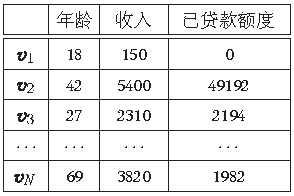
\includegraphics[width=0.45\hsize]{ldp_range_query/figures_others/multi-dimensionalDataset.pdf}
    \vspace{-0.2cm}
    \caption{示例数据集包含 $N$ 个用户以及每个用户的三个属性值:年龄,收入和已贷款额度} 
    \label{Example dataset}
    \vspace{-0.3cm}
\end{figure}

% Assume there are $N$ users, where the $i$-th user has an $m$-dim ordinal record ${\bf{v}}^{m}_i = (v^{(1)}_i, v^{(2)}_i, \cdots, v^{(m)}_i)$, with $v_i^{(j)}$ representing the $j$-th private attribute value owned by user $i$. 
假设参与数据收集的有 $N$ 个用户,其中第 $i$ 个用户拥有一个 $m$ 维数据记录 ${\bf{v}}^{m}_i = (v^{(1)}_i, v^{(2)}_i, \cdots, v^{(m)}_i)$,其中 $v_i^{(j)}$ 表示用户 $i$ 拥有的第 $j$ 维的属性值。
将第 $j$ 个属性值的数据域表示为 $D_j$,
给定一系列范围 $\alpha_j$,$\beta_j$($j=1,2,\cdots,m$),可以计算出一个 $m$ 维范围查询结果。
\begin{equation}
    R_{\bigcap {[\alpha_j,\beta_j]}_{j=1}^{m}}=\frac{1}{N} \sum_{i=1}^{N} \mathbb{I}_{\bigcap{\{\alpha_j \leq v_i^{(j)} \leq \beta_j\}_{j=1}^{m}}}
\end{equation}
其中 $\mathbb{I}_\phi$ 是一个指示函数,如果谓词 $\phi$ 成立则取值为1,否则为0。
% For example, the proportion of people within 20 years to 40 years old constitutes a 1-dim range query, 
% while the ratio of people within 20 years to 40 years old, with salary less than 5000, and with loan amount less than 20000 constitutes a 3-dim range query, 
% where the three dimensions corresponding to age, salary and loan amount, respectively.
\autoref{Example dataset} 给出了一个范围查询的运行示例。
例如,统计年龄在20岁到40岁之间的用户在群体中所占比例是一个一维范围查询,
而统计同时满足年龄在20岁到40岁之间、工资低于5000元和已贷款金额低于20000元的用户在群体中所占比例是一个三维范围查询。

\subsection{分层-间隔优化方法(\myhio)}
\label{exsitingHIO}
基于$B$叉树,\myhio \cite{wang2019answering}将整个数据域分解成互不相交的子集,称为“间隔”。
根节点表示整个数据域,叶节点表示单个值。同一层上的节点表示相同粒度的间隔。然后,\myhio 通过\oue \cite{wang2017locally}算法获得每层节点的频率估计。
当回答范围查询时,\myhio 使用来自不同层的最少间隔完全覆盖查询范围。
例如,当用户的私有属性域大小$|D|=8$,树分支因子$B=2$时,范围查询$[2,7]$可以分解为间隔$[2,3] \cup [4,7]$。
然后,\myhio 将上述两个间隔的估计频率值相加,以回答范围查询。
对于长度为$r$的一般查询,\myhio 最多可以使用$2(B-1)\log_B|D|$个间隔来回答。
与直接使用\fo 机制相比,\myhio 在回答查询时可以有效地减少使用的间隔数量,从而大大减少由于在范围内添加嘈杂的频率值所引起的累积误差。

但是,\myhio 存在两个限制其在实践中适用性的弱点。
1)\myhio 将相同水平的噪声插入到所有间隔的估计频率中。对于间隔较小的节点,扰动噪声往往会掩盖真实频率值,从而降低整个算法的效用。
2)在多维场景中,树层数随维数指数增加。对于高维场景,查询误差随着过多的小值节点而明显地增加。

\subsection{离散哈尔小波变换方法(\mydht)}
\label{exsitingDHT}
\mydht \cite{cormode2019answering} 在域上施加完全二叉树结构,并将用户私有值 $v$ 编码为一组哈尔小波系数。 
\mydht 的动机是,在长度为 $r$ 的范围查询中,相比直接应用\fo ,使用哈尔小波域中估计的值数量更少。

\mydht 也面临一些限制:
1)与 \myhio 相似,\mydht 将相同级别的噪声插入到所有估计的哈尔小波系数中。
对于一些数值较低的系数,噪声倾向于使估计系数偏离实际值,导致查询误差增加;
2)它主要设计用于一维场景,因此在实际应用中存在限制。


\subsection{高维边缘列联表发布方法(\mycalm)}
\label{Consistent Adaptive Local Marginal}
\mycalm \cite{zhang2018calm} 是一种边缘列联表发布 LDP 协议,可在保护隐私的同时构建 $m$ 个属性的联合分布。
\mycalm 不是直接估计包含所有属性边际表,而是根据用户数据域的大小和数据维度的数量进行策略性的属性组合统计,基于属性组合的统计结果可以重建包含所有属性的边际表。
我们注意到,\mycalm 可以用于回答范围查询。
更具体地,为了回答一个多维范围查询,\mycalm 可以将查询包含的重建的边际值求和。

然而,当域大小 $|D|$ 很大时,\mycalm 需要将大量经过扰动的边际值求和以回答范围查询,这可能会向结果中引入过量的噪声。

\subsection{混合维度网格方法(\myHDG)}
\myHDG \cite{yang2020answering}是在LDP场景下回答多维范围查询的现有最好方法。
\myHDG 首先将用户所有属性进行两两组合形成二维数据域,然后基于用户数据域大小将二维数据域精心分桶成粗略的二维网格,并统计每个子数据域内的用户频率。
之后,\myHDG 基于二维范围查询的结果估计出更高维范围查询结果。
为了刻画用户数据的细粒度分布信息,\myHDG 使用粒度更细的一维网格统计每个用户属性的频率分布信息,并结合来自一维和二维网格的信息来回答高维范围查询。

然而,\myHDG 存在下列缺陷:
1) \myHDG 的等粒度网格无法处理各种分布的用户数据。
对于分布较为偏斜的数据集,其用户数据集中在整个数据域的一小部分。因此,在某些网格中噪声误差或非均匀误差会占主导地位,从而降低结果精度;
2) 使用一维网格可能会破坏用户数据中不同属性之间的相关性。

\subsection{总结}
\label{Remarks}

为了克服现有低维机制(\myhio、\mydht)和高维机制(\mycalm、\myHDG)的局限性,我们旨在实现以下两个设计目标:
1)找到合理的区间分解方法,避免引入过多的噪声;
2)设计的机制可以扩展到多维场景,比现有算法具有更好的查询精度。
在这些目标的推动下,我们提出了\myahead,与现有工作存在以下主要差异:
1)与现有方法采用的静态数据编码机制相比,\myahead 采用的是一种自适应、动态的数据编码机制;
2)\myahead 通过合并区间减少噪声对小值节点的影响;
3)所设计的机制可以从一维迁移到多维场景。
接下来,我们将详细阐述\myahead 的动机和设计。

\section{本文方法(\myahead)}
\label{Adaptive Hierarchical Decomposition}

\subsection{设计思路}
\label{Motivation and Overview}
\begin{figure}[!t]
    \centering
    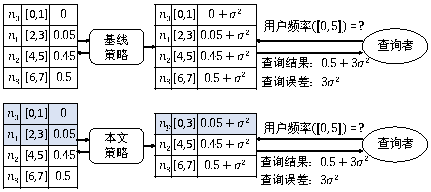
\includegraphics[width=0.75\hsize]{figure/ldp_range_query/figures_others/Motivation3ch.pdf}
    % \vspace{-0.2cm}
    \caption{基线策略与自适应策略}
    \label{Method Motivation}
    % \vspace{-0.3cm}
\end{figure} 

\begin{figure*}[t]
    \centering
    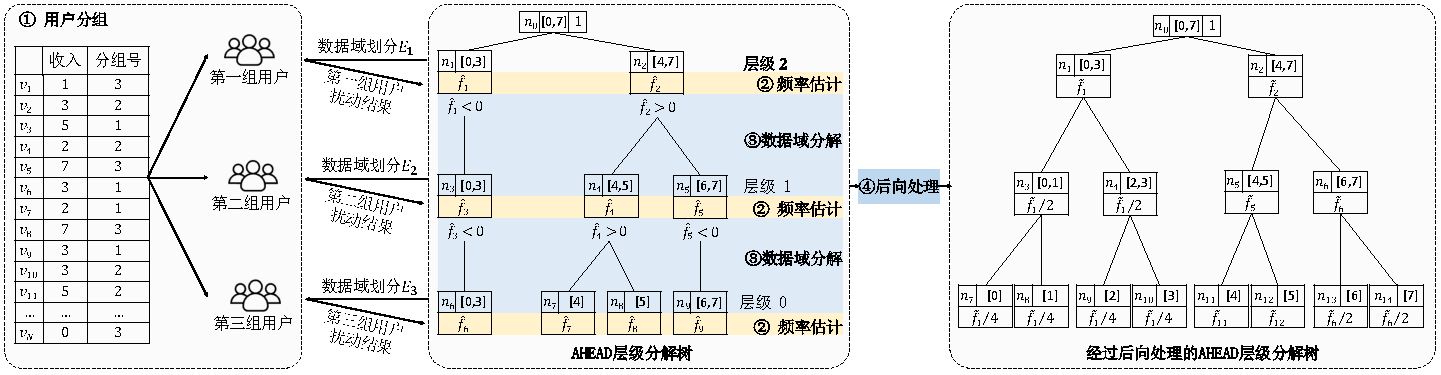
\includegraphics[width=\hsize]{figure/ldp_range_query/figures_others/OverviewAHEAD4ch.pdf}
    % \vspace{-0.4cm}
    \caption{\myahead 的工作流程。从左到右依次展示了\myahead 算法中的四个步骤,即用户分组、频率估计、数据域分解和后向处理。 
    \myahead 根据右侧子图中的树回答范围查询。} 
    \label{AHEAD method}   
    % \vspace{-0.4cm}
\end{figure*}

在这个章节中,我们使用一个例子来说明现有算法的局限性以及\myahead 的合理性。
如\autoref{Method Motivation}所示,左侧的表格显示了带有相应实际频率值的数据区间。
例如,区间$[0,1]$的真实频率值为$0$,意味着这个区间内没有用户数据。
然后,中间的表格显示了使用不同策略分别估计的区间频率值。
其中,$\sigma^2$代表扰动过程中引入的噪声方差。
右侧的剩余部分展示了基于估计值回答查询的过程。

首先,我们关注基线策略,例如\myhio。
基线策略选择发布每个区间的估计频率值。
每个估计值通过\fo 机制引入了“噪声误差”,以满足LDP的要求。
对于区间$[0,1]$,它的真实值为$0$,这意味着这些区间的估计值完全被噪声填充。
当回答范围查询时,例如区间$[0,5]$的用户频率,提问者想知道区间$[0,5]$的频率值。
基线策略的结果是$0.5 + 3\sigma^2$。
在这个例子中,区间$[0,1]$的真实值并未对查询答案做出贡献,却带来了同等程度的噪声,降低了基线策略的查询准确度。

另一方面,对于自适应策略,如果我们知道各区间的真实频率值,就可以合并区间$n_0$和$n_1$,只需要估计合并后的区间$n_p$。
当需要输出区间$[0,5]$的用户频率时,自适应策略的结果是$0.5 + 2\sigma^2$,与基线方法相比,将噪声误差降低了30\%。

自适应策略可以有效减小扰动噪声对频率值较小区间的影响。
但是,当查询需要使用合并区间的部分区域时,自适应策略必须通过对合并区间内频率分布的作出假设才能进行后续的计算。
主流方法是假设合并区间内的频率分布满足均匀分布\cite{ioannidis2003history},即合并区间用户频率均匀分布。
如果实际用户频率不满足该假设时,自适应策略的结果将会产生“非均匀误差”。
例如,如果查询者想要知道区间$[2,3]$的用户频率,那么自适应策略将基于两个区间的尺寸在均匀分布的假设下进行计算,即 $[0,3]$ 区间频率值的一半。
与基准策略相比,自适应策略将噪声误差从 $\sigma^2$ 降低到 $\frac{\sigma^2}{2}$,
同时它也带来了非均匀误差 $0.05 - \frac{0.05}{2} = 0.025$。

自适应性通过合并区间来减少噪声误差,同时通过假设均匀分布引入了非均匀误差。
因此,我们希望找到最优的数据域分解来平衡这两种误差,进而减少总查询误差。
文献\cite{muthukrishnan1999rectangular}指出即便是在二维数据场景下,找到最优的数据域分解是困难的,那么在隐私约束下这个问题将变得更具挑战性。 
综上,我们提出了一种基于自适应层级递归划分策略(详见\autoref{Workflow of ahead}),旨在平衡噪声误差和非均匀误差,并解决现有方法的不足。

\subsection{一维数据场景\myahead 的工作流程}
\label{Workflow of ahead}
在本章,我们通过\autoref{AHEAD method}中的例子阐述\myahead 的工作流程。
聚合器希望基于\myahead 完成有关用户收入的范围查询任务。
收入数据被分成了8个有序级别,即域大小$|D|=8$。
树的扇出度$B=2$,这意味着\myahead 树的每个节点最多有两个子节点。
在\myahead 原型树的每个节点中,$n_i$表示节点索引,$[a,b]$表示节点的区间,$\hat{f_i}$表示估计的频率值。
值得注意的是,\myahead 采用了抽样原则\cite{cormode2019answering},将全部参与用户划分为子用户组,每组用户使用全部隐私预算。
抽样原则可以显著减少本地差分隐私场景中查询结果的噪声误差\cite{nguyen2016collecting, wang2017locally, wang2019locally}
% (有关更多详细信息,请参见\autoref{The rationality of sampling principle})。
接下来,我们将\myahead 的工作流程分为四个步骤。

\mypara{第一步:用户分组}
如\autoref{AHEAD method}中所示的左虚线框中,
聚合器确定分区数$c$,其中$c=\log_B|D|$旨在确保将用户分配到\myahead 树的每一层。
用户随机选择在范围$[1,2,3,\cdots,c]$内的组号。
此外,用户还可以利用他们的公共信息来选择组,例如帐户注册时间,用户ID等。
分区过程应确保每个组代表整体人口,具有相似数量的用户。

\mypara{第二步:频率估计}
在中间的虚线框中,聚合器首先建立代表整个数据域的根节点$n_0$。
然后,聚合器对域进行初始分解,即将整个域分成$B$个相等大小的区间,然后将区间节点连接到根节点$n_0$上。
根节点的子节点代表一种将整个数据域分割的方法,表示为数据域分解$E_1$。
聚合器选择第一组用户,并向他们发送分解$E_1$和隐私预算$\epsilon$。
第一组用户中的每个用户将自己的私有值$v$投影到$E_1$的区间上,并通过\oue 上传$v$的投影值。在接收到用户报告后,聚合器使用聚合算法获得估计的频率分布$\hat{F_1}$,表示落在每个节点区间内的用户比例。

\mypara{第三步:数据域分解}
聚合器将$\hat{F_1}=\{\hat{f_1}, \hat{f_2}\}$的每个频率值与阈值$\theta$进行比较,并决定是否进一步分割$E_1=\{[0,3], [4,7]\}$中的相应区间。
具体来说,由于$\hat{f_2}$大于设定的$\theta$,因此应将$E_1$中的相应区间$[4,7]$分成$B$个大小相等的子区间$[4,5]$和$[6,7]$。
而节点$n_1$的频率值$\hat{f_1}$小于$\theta$,那么区间$[0,3]$不需要进一步划分。
对于新的区间节点,我们将它们附加到相应的父区间节点上。
当$\hat{F_1}$中的所有元素都被遍历时,我们可以获得一组新的数据域分解$E_{2}$。

然后,聚合器将分解$E_{2}$发送给第二组用户并获得估计的频率分布$F_2$。聚合器重复以上步骤,直到应用所有用户组并获得\autoref{AHEAD method}中显示的\myahead 原型树。由于估计频率小于阈值$\theta$,\myahead 不会在后续交互中分解区间$[0,3]$和$[6,7]$。
为了满足LDP要求,区间$[0,3]$和$[6,7]$依然参与后续用户组的频率估计。

在构建原型树时,\myahead 分别估计每个层的频率分布。
在这个过程中,\myahead 没有考虑树中频率值的约束,例如子节点的频率值之和等于其父节点。
因此,在步骤四中,我们通过对节点估计进行“非负性”和“加权平均”处理,来进一步提高\myahead 查询结果的准确性。

\mypara{第四步:后向处理}
% 后向处理包含两个步骤:非负性和加权平均。
首先是对节点频率值进行非负性处理,\myahead 使用Norm-Sub \cite{wang2019consistent}对同一层中的节点进行处理,以确保节点的估计频率为非负数且频率总和为1。
\myahead 将负值转换为0,并计算正值的总和与1之间的差异。
接下来,每个正值减去平均差异,该平均差异是通过将总差异除以正估计值的数量获得的。
非负性处理过程重复进行,直到所有节点的频率值都变为非负数。

然后\myahead 从下往上对所有节点的频率值进行加权平均。
\myahead 计算非叶节点$n$和其子节点频率值的加权平均值,以更新$n$的估计频率,即通过融合$n$的多个估计结果来降低扰动噪声的影响。

\begin{equation}
    \label{weighted average}
    \tilde{f}(n)=\left\{
    \begin{array}{rcl}
    \lambda_1\hat{f}(n) + \lambda_2 \sum_{u \in child(n)}\hat{f}(u), &   \mbox{如果$u$是一个叶子节点} \\
    \lambda_1\hat{f}(n) + \lambda_2 \sum_{u \in child(n)}\tilde{f}(u),    & \mbox{其他情况}  \\
    \end{array}\right.
\end{equation}

权重 $\lambda_1$ 和 $\lambda_2$ 与估计值的方差成反比,即 $\lambda_1 = \frac{\myvar_{child(n)}}{\myvar_{child(n)} + \myvar_{(n)}}$ 和 $\lambda_2 = \frac{\myvar_{(n)}}{\myvar_{child(n)} + \myvar_{(n)}}$,其中 $\myvar_{child(n)}$ 表示节点 $n$ 的子节点方差之和,$\myvar_{n}$ 表示节点 $n$ 的方差。
$\tilde{f}$ 表示 $\hat{f}$ 的后向处理版本,将用于回答查询。
% 加权平均过程可以最小化噪声的幅度,如下定理所示。 \autoref{theorem: weighted average} 的证明可以在 \autoref{The proof of weighted average} 中找到。

\begin{theorem}
    \label{theorem: weighted average}
    使用{\rm\autoref{weighted average}}来更新节点的频率,节点$n$可以达到最小扰动方差。
\end{theorem} 
\begin{proof}
    根据文献{\rm\parencite{wanglocally}},经过扰动后的区间估计频率值$\hat{f}$近似于$f+X$,其中$f$是真实的频率值,$X$是一个服从\Gaussian 分布$\mathcal{N}(0,\myvar_{\oue})$的随机变量。
    假设$u$为叶子节点,那么有
    \begin{align}
    \hat{f}(n) = f(n) + \mathcal{N}(0,\myvar_{(n)}) \nonumber
    \end{align}
    \begin{align}
    \sum_{u \in child(n)} \hat{f}(u) = \sum_{u \in child(n)}f(u) + \mathcal{N}(0,\myvar_{(u)}) \nonumber
    \end{align}
    节点$n$的区间等于其子节点区间的组合。因此
    \begin{align}
    f(n) = \sum_{u \in child(n)}f(u) \nonumber
    \end{align}
    设加权平均的系数为$\lambda_1$和$\lambda_2$,$f(n)$和$\sum_{u \in child(n)}f(u)$之间的加权平均值是节点$n$频率的无偏估计,其中$\lambda_1+\lambda_2=1$。
    \begin{align}
    \tilde{f}(n)=\lambda_1\hat{f}(n)+\lambda_2\sum_{u \in child(n)}\hat{f}(u) \nonumber
    \end{align}
    $\tilde{f}(n)$的方差等于$\lambda_1^2\myvar_{(n)}+\lambda_2^2\myvar_{child(n)}$。
    当且仅当
    \begin{align}
    \lambda_1=\frac{\myvar_{child(n)}}{\myvar_{child(n)}+\myvar_{(n)}} \nonumber,~~~~
    \lambda_2=\frac{\myvar_{(n)}}{\myvar_{child(n)}+\myvar_{(n)}},\nonumber
    \end{align}
    我们可以最小化$\tilde{f}(n)$的方差。
    加权平均后,扰动噪声仍服从\Gaussian 分布。
    因此,当$u$不是叶子节点时,上述证明仍然成立。
\end{proof}

最后,从根节点到叶子节点,\myahead 基于均匀分布假设递归地分解父节点的频率值,并获取完整的层级分解树以回答范围查询,具体如\autoref{AHEAD method} 的最右边子图所示。

\begin{algorithm}[!htbp]
	\begin{algorithmic}[1]
        \REQUIRE 用户私有值 $V=\{v_1, \ldots, v_N\}$,数据域 $D$,树扇出度 $B$,隐私预算 $\epsilon$,阈值 $\theta$。
        \ENSURE 经过后向处理的\myahead 层级分解树 $T$
		\STATE $c = {\log_B}|D|$
		\STATE $//$ 用户划分
        \STATE 随机将所有用户划分为 $c$ 个用户组 $\left\{ V_1, V_2, \ldots, V_c \right\}$
        \STATE 创建表示整个数据域的树 $T$的根节点 $e^0_0 = [1, |D|]$,并初始化其频率值$T.\operatorname{node}(e^0_0).\operatorname{frequency} = 1$
		\FOR {$i$ from 1 to $c$}
            \STATE $//$ 数据域分解
            \FOR {$j$, node in enumerate($T.\operatorname{node}(\operatorname{level}=i-1)$)}
            \IF {$\operatorname{node.frequency} > \theta$}
            \STATE 将区间 $e^{i-1}_j$ 分解为 $B$ 个不相交的子区间 $\{e^{i-1}_{j,k}\}$
            \FOR {$k$ from $1$ to $B$}
    		\STATE $\operatorname{node.add\_child}(e^{i-1}_{j,k})$
            \ENDFOR
            \ELSE
            \STATE $\operatorname{node.add\_child}(e^{i-1}_{j})$
            \ENDIF    		
            \ENDFOR
            \STATE $//$ 频率估计
            \STATE $F = \fo(V_i, T.\operatorname{node}(\operatorname{level}=i).\operatorname{interval}, \epsilon)$
            \FOR {$k$, node in enumerate $T.\operatorname{node}(level=i)$}
    		\STATE $\operatorname{node}.\operatorname{frequency} = F[k]$
            \ENDFOR
        \ENDFOR
        \STATE $//$ 后向处理
        \STATE 运行 \autoref{alg:1-dim post_processing}
        \STATE 返回 $T$
	\end{algorithmic}
    \caption{构建一维\myahead 层级分解树}
    \label{Construct 1-dim prototype tree}
\end{algorithm}

\begin{algorithm}[!ht]
	\caption{后向处理}
	\label{alg:1-dim post_processing}
	\begin{algorithmic}[1]
        \REQUIRE \myahead 层级分解树 $T$, 树扇出度 $B$
        \ENSURE 经过后向处理的\myahead 层级分解树 $T$
        \FOR {$i$ from $1$ to $c$}
		\STATE norm\_sub($T.\operatorname{node}(\operatorname{level}=i).\operatorname{frequency}$)
        \ENDFOR    
        \FOR {$j$ from $c-1$ to $1$}
            \FOR {\_, node in enumerate $T.\operatorname{node}(\operatorname{level}=j)$}
            \STATE $f_1$ = $\operatorname{node}.\operatorname{frequency}$, $f_2$ = $\sum{\operatorname{node.children().frequency}}$
		    \STATE $\operatorname{node}.\operatorname{frequency}$ = $\lambda_1$$f_1$ + $\lambda_2$$f_2$
            \ENDFOR 
        \ENDFOR    
        \FOR {$k$ from $1$ to $c$}
            \FOR {\_, node in enumerate $T.\operatorname{node}(\operatorname{level}=k)$}
                    \IF {$\operatorname{node}.\operatorname{children()}$ == None}
		            \STATE $\operatorname{node}.\operatorname{add\_children}()$
		            \STATE $\operatorname{node}.\operatorname{children()}.\operatorname{frequency} = \operatorname{node}.\operatorname{frequency}/B$
                    \ENDIF
            \ENDFOR 
        \ENDFOR    
    \end{algorithmic}
\end{algorithm}

\subsection{高维数据场景\myahead 的工作流程}
\label{Extension to Multi-dimensional Settings}
\subsubsection{二维数据场景}

首先我们讨论二维数据场景。
我们假设所有属性都具有相同的域 $D = \{1, 2, \cdots, d\}$,
其中 $d$ 是树扇出度 $B$ 的幂。
如果实际用户的数据域不同,我们可以添加一些填充值使所有数据域长度一致。
一维数据场景和二维数据场景的主要区别在于分解过程,体现在\autoref{Construct 1-dim prototype tree} 的第4行和第9行。
对于一维数据场景,\myahead 按层次划分整个数据域 $[1, |D|]$。
整个数据域划分为粒度不同的子区间。
对于二维数据场景,整个数据域变成了一个正方形区域 $[1, |D|] \times [1, |D|]$。
所以,\myahead 需要生成不同粒度的二维网格来分解整个数据域。
我们在\autoref{Multi-dimensional tree}给出了二维数据场景的\myahead 的工作流程,并在\autoref{Construct 2-dim prototype tree} 提供了相应的伪代码。
在上述示例中,用户私有属性的数据域大小为 $8\times8$,树扇出度 $B=4$。
与一维数据场景类似,二维\myahead 也需要四个步骤来估计用户的频率分布。

\mypara{第一步:用户分组}
用户在 $\{1, 2, 3, \cdots, c\}$ 的集合中随机选择用户组编号,其中 $c = \log_B|D|^2$。

\mypara{第二步:频率估计}
接着,聚合器将整个数据域划分为 $B$ 个等大小的正方形区域,并将初始数据划分发送给第一组用户。
用户将其私有数据投影到初始划分中,并通过 \oue 上传其数据。
服务器使用聚合算法获取估计的频率分布,该分布表示落入每个子域内的用户比例。

\mypara{第三步:数据域分解}
然后,聚合器将每个估计频率值与阈值 $\theta$ 进行比较,决定是否进一步划分相应的子域。
重复频率估计和数据域分解过程,\myahead 递归地分解域并构建 \myahead 原型树。

\mypara{第四步:后向处理}
最后,\myahead 在每个层内执行非负性处理,并在两个相邻层之间执行父节点和子节点估计频率之间的加权平均,以进一步减小估计误差。
基于均匀分布假设,\myahead 得到完整的树结构来回答范围查询。

因为查询结果的误差随使用节点数量的增加而增加,为了减少查询误差,\myahead 更倾向于使用粗粒度节点来回答查询。
如\autoref{Multi-dimensional tree} 所示,\myahead 回答一个二维查询 $[0,5]\times[0,5]$。 
\myahead 从树的顶层向下搜索,并计算范围查询完全覆盖的子域的频率之和。
范围查询完全覆盖了顶层 $[0,3]\times[0,3]$ 的区域以及中间层的五个区域 $[0,1]\times[4,5]$、$[2,3]\times[4,5]$、$[4,5]\times[4,5]$、$[4,5]\times[0,1]$、$[4,5]\times[2,3]$(这些区域用蓝色突出显示),
因此查询答案为 $(\tilde{f}1 + \tilde{f}9 + \tilde{f}{11} + \tilde{f}{13} + \tilde{f}{14} + \tilde{f}{4}/4)$。

对于二维范围查询,我们设置$B=2^2$,即每个维度的树扇出度为$2$。
作为比较,我们在实验中还给出了$B=4^2$的结果。
由于$\theta$的推导不涉及维度变化,
因此我们仍然根据\autoref{theta setting1}选择$\theta$。

\begin{algorithm}[!htbp]
    \caption{构建二维\myahead 层级分解树}
    \label{Construct 2-dim prototype tree}
	\begin{algorithmic}[1]
        % \REQUIRE All users’ value set $V = \{v_1, v_2,\ldots,v_N \}$, attribute domain $D$, tree fanout $B$, privacy budget $\epsilon$, threshold $\theta$
        % \ENSURE \myahead Tree $T$
        \REQUIRE 用户私有值 $V=\{v_1, \ldots, v_N\}$,数据域 $D$,树扇出度 $B$,隐私预算 $\epsilon$,阈值 $\theta$。
        \ENSURE 经过后向处理的\myahead 层级分解树 $T$
		\STATE $c = {\log_B}|D|^2$
        \STATE $//$ 用户划分
        % \STATE Randomly divide users into $c$ parts $\left\{ V_1, V_2, \ldots, V_c \right\}$
        % \STATE Create the root node of tree $T$ with initial interval $e^0_0 = [1, |D|] \times [1, |D|]$ and $\operatorname{T.node}(e^0_0).frequency = 1$ 
        \STATE 随机将所有用户划分为 $c$ 个用户组 $\left\{ V_1, V_2, \ldots, V_c \right\}$
        \STATE 创建表示整个二维数据域的树 $T$的根节点 $e^0_0 = [1, |D|] \times [1, |D|]$ 和 $\operatorname{T.node}(e^0_0).\operatorname{frequency = 1}$
		\FOR {$i$ from 1 to $c$}
            \STATE $//$ 数据域分解
            \FOR {$j$, node in enumerate($T.\operatorname{node}(\operatorname{level}=i-1)$)}
            \IF {$\operatorname{node.frequency} > \theta$}
            % \STATE Divide $\operatorname{interval} e^{i-1}_j$ into $B$ disjoint intervals $\{e^{i-1}_{j,k}\}$
            \STATE 将二维区间 $e^{i-1}_j$ 分解为 $B$ 个不相交的二维子区间 $\{e^{i-1}_{j,k}\}$
            \FOR {$k$ from $1$ to $B$}
    		\STATE $\operatorname{node.add\_child}(e^{i-1}_{j,k})$
            \ENDFOR
            \ELSE
            \STATE $\operatorname{node.add\_child}(e^{i-1}_{j})$
            \ENDIF 		
            \ENDFOR

            \STATE $//$ 频率估计
            \STATE $F = \fo(V_i, T.\operatorname{node}(\operatorname{level}=i).\operatorname{interval}, \epsilon)$
            \FOR {$k$, node in enumerate $T.\operatorname{node}(\operatorname{level}=i)$}
    		\STATE $\operatorname{node}.\operatorname{frequency} = F[k]$
            \ENDFOR
        \ENDFOR
        \STATE $//$ 后向处理
        \STATE 运行 \autoref{alg:1-dim post_processing}
        \STATE 返回 $T$
	\end{algorithmic}
\end{algorithm}

\subsubsection{三维及以上数据场景}

\myahead 可以通过两种方式扩展到更高维度。

\mypara{直接估计算法(Direct Estimation,\de)}
基于扇出度为 $B=2^m$ 的树,\myahead 同时分解 $m$ 个维度。
例如,\myahead 将三维域视为一个立方体,然后聚合不同粒度的子立方体的频率以回答查询。
在 \autoref{theta setting1} 的阈值设置下,\myahead 可以很好地控制子域的整体估计误差。
然而,叶节点数目随着维度呈指数级增长,这使得在高维数据集上查询答案过程非常耗时。

\mypara{利用低维估计算法(Leveraging Low-dimensional Estimation,\lle)}
为了解决数据维度上升引起的子域爆炸问题,
\lle 首先将属性两两配对,然后为每个属性对构建一个二维\myahead 树。
接着,在回答一个 $m$ 维查询时,\lle 构建一个包含 $2^m$ 个关联查询的查询集合。
最后,利用二维频率作为约束条件,\lle 通过最大熵优化估计所有 $2^m$ 个查询的频率值。
接下来,我们将详细介绍\lle 方法的三个步骤。
\begin{enumerate}
\item [1)] \mypara{构建二维树} \myahead 将所有属性成对分组,形成 $C_m^2$ 个二维属性对。
然后,\myahead 分别为这 $C_m^2$ 个二维属性对进行二维频率分布估计,即总共构建了 $C_m^2$ 个二维树。
\item [2)] \mypara{属性分布对齐} 
\myahead 需要在二维树集合中进行 $m$ 个数据维度的边际分布的对齐。
这保证了从不同二维树中进行某一属性的范围查询时结果的唯一性。
例如,属性 $a$ 参与了 $(m-1)$ 个属性对。
假设这 $(m-1)$ 个二维树分别为 $\{T_1, T_2, T_3, \cdots, T_{m-1}\}$,每个树除了根节点外都有 $\ell$ 层。
对于整数 $k \in [1, B^{\ell/2}]$,我们定义 $f_{T_i}(a, \ell, k)$ 为属于第 $\ell$ 层的 $T_i$ 节点的频率之和,
这些节点所对应的子域在属性 $a$ 上的覆盖范围为 $[(k-1)\cdot\frac{|D|}{B^{\ell/2}}+1, k\cdot\frac{|D|}{B^{\ell/2}}]$。
为了使所有 $f_{T_i}(a, \ell, k)$ 的频率分布在属性$a$的边际分布上保持一致,
\myahead 计算它们的加权平均值 $f(a, \ell, k) = \sum_{i=1}^{m-1}\lambda_{i} \cdot f_{T_i}(a, \ell, k)$,
其中 $\lambda_i$ 是 $f_{T_i}(a, \ell, k)$ 的权重,且 $\sum_{i=1}^{m-1}\lambda_i = 1$。
设置的权重值 $\lambda$ 用来最小化 $f(a, \ell, k)$ 的方差,
即 $\myvar[f(a, \ell, k)] = \sum_{i=1}^{m-1}\lambda_i^2\cdot \myvar[f_{T_i}(a, \ell, k)]$,其中 $\myvar[f_{T_i}(a, \ell, k)]$ 是用于计算 $f_{T_i}(a, \ell, k)$ 的节点理论方差之和。
当权重与估计值的方差成反比时,$\myvar[f(a, \ell, k)]$ 最小\cite{yang2020answering}。
因此,最优权重 $\lambda_i = \frac{1}{\myvar[f_{T_i}(a, \ell, k)]}/\sum_{i=1}^{m-1}\frac{1}{\myvar[f_{T_i}(a, \ell, k)]}$。
我们通过在原始估计频率上添加 $(f(a, \ell, k) - f_{T_i}(a, \ell, k))/B^{\ell/2}$ 来更新 $T_i$ 中原有的频率估计值,最终使每个 $f_{T_i}(a, \ell, k)$ 等于 $f(a, \ell, k)$。
根据文献{\rm\parencite{qardaji2014priview}} 的分析结论,
关于属性 $a$ 在 $\{T_1, T_2, T_3, \cdots, T_{m-1}\}$ 进行属性分布对齐不会影响其他属性的频率分布。
% ${T_1, T_2, T_3, \cdots, T_{m-1}}$ 在不改变的情况下达成对 的一致。
因此,我们可以按任意属性顺序进行属性分布对齐,\myahead 可以实现所有 $m$ 个属性的一致性。注意到每个二维树有 $\ell$ 层,\myahead 需要对所有 $\ell$ 层分别执行属性分布对齐。
\item [3)] \mypara{最大熵优化} 
我们采用了最大熵原理\cite{qardaji2014priview},基于二维查询的结果估计 $m$ 维查询结果。
具体来说,对于一个 $m$ 维范围查询 $q$,我们可以定义一组范围查询:
$$Q(q)=\left\{\wedge\left(a_{j},\left[\alpha_{j}, \beta_{j}\right] \text { or }\overline{\left[\alpha_{j}, \beta_{j}\right]}\right) \mid a_{j} \in A\right\}\text{,}$$
其中 $[\alpha_t, \beta_t]$ 表示查询区间,$\overline{\left[\alpha_{t}, \beta_{t}\right]}$ 是其补集。
对于 $2^m$ 个查询 $g \in Q(q)$,
我们定义 $f_q(g)$ 为 $Q(q)$ 查询结果集合。
我们可以获得 $Q(q)$ 对应的二维查询集合以及其对应的查询结果集合$f_{q^{(j,k)}}$:
$$Q(q^{(j,k)})=\left\{\left(a_{j},\left[\alpha_{j}, \beta_{j}\right] \text { or }\overline{\left[\alpha_{j}, \beta_{j}\right]}\right) \wedge \left(a_{k},\left[\alpha_{k}, \beta_{k}\right] \text { or }\overline{\left[\alpha_{k}, \beta_{k}\right]}\right)\right\}\text{,}$$
对于任何查询 $g^{(j,k)} \in Q(q^{(j,k)})$,我们使用 $f_{q^{(j,k)}}(g^{(j,k)})$ 来表示其查询结果。
例如,对于一个 $g^{(j,k)} \in Q(q^{(j,k)})$,$f_{q}(g^{(j,k)})$ 表示通过对 $Q(q)$ 集合中的查询结果求和,以构建高维查询 $g^{(j,k)}$ 的结果 $f_q$。
接着,我们可以通过求解下列优化问题得到具体的高维查询结果。
$$
\begin{array}{ll}
\text { maximize } & -\sum_{g \in Q(q)} f_{q}(g) \cdot \log \left(f_{q}(g)\right) \\
\text { subject to } & \forall_{g \in Q(q)} f_{q}(g) \geq 0 \\
& \forall_{a_j, a_k \in A} \forall_{g^{(j, k)} \in Q\left(q^{(j, k)}\right)} f_{q^{(j, k)}}(g^{(j, k)})=f_{q}(g^{(j, k)})
\end{array}
$$
以上优化问题可以通过现有凸优化工具来解决。
为了更快速的计算出查询结果,降低查询延迟,\myahead 采用文献{\rm\parencite{yang2020answering}}提出的加权更新算法,
该算法在降低计算复杂度的同时实现了与最大熵估计相当的精度。
\end{enumerate}

\de 方法的实现相对简单,而且用户分区的数量不会随着维数的增加而增加。然而,\de 中的 \myahead 树在高维情况下可能非常大,从而使得树的构建和查询回答过程变得耗时。
相比之下,\lle 方法将属性成对组合,为每个属性对构建一个二维 \myahead 树,使得每棵树的规模不会太大。
% 我们在 \autoref{Effectiveness of ahead for high-dimensional Range Query} 中从经验上展示了这两种策略的性能,并讨论了如何在它们之间进行选择。
% 之前的方法也利用最大熵优化将低维机制有效地扩展到高维场景中。例如,\PriView\cite{qardaji2014priview} 提出构建低维视图,即二维、三维边缘表,并将最大熵优化应用于从视图中重建更高维的边缘表。

% \begin{algorithm}[!h]
% 	\caption{Post-processing}
% 	\label{alg:2-dim post_processing}
% 	\begin{algorithmic}[1]
%         \REQUIRE \myahead tree $T$, tree fanout $B$
%         \ENSURE \myahead tree $T$
%         \FOR {$i$ from $1$ to $c$}
% 		\STATE norm\_sub($T.\operatorname{node(level=i)}.\operatorname{frequency}$)
%         \ENDFOR    
%         \FOR {$j$ from $c-1$ to $1$}
%             \FOR {\_, node in enumerate $T.\operatorname{node}(level=j)$}
%             \STATE $f_1$ = node.frequency, $f_2$ = $\sum{\operatorname{node.children().frequency}}$
% 		    \STATE node.frequency = $\lambda_1$$f_1$ + $\lambda_2$$f_2$
%             \ENDFOR 
%         \ENDFOR    
%         \FOR {$k$ from $1$ to $c$}
%             \FOR {\_, node in enumerate $T.\operatorname{node}(level=k)$}
%                     \IF {node.children() == None}
% 		            \STATE $\operatorname{node}.\operatorname{add\_children}()$
% 		            \STATE $\operatorname{node}.\operatorname{children()}.\operatorname{frequency} = \operatorname{node}.\operatorname{frequency}/B$
%                     \ENDIF
%             \ENDFOR 
%         \ENDFOR    
        
%     \end{algorithmic}
% \end{algorithm}

\begin{figure*}[t]
    \centering
    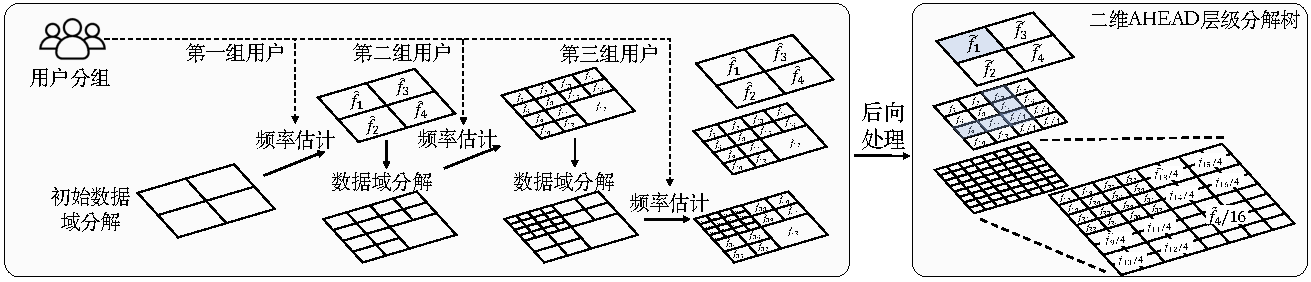
\includegraphics[width=\hsize]{figure/ldp_range_query/figures_others/GridAHEAD_workflow2ch.pdf.pdf}
    \vspace{-0.7cm}
    \caption{
        % 2-dim \myahead algorithm, 
    % where the decomposition is implemented by decomposing both dimensions simultaneously.
    \myahead 构建二维层级分解树的流程。在数据域分解过程中,\myahead 同时对二维数据域的两个维度同时进行分解。}
    \vspace{-0.4cm}
    \label{Multi-dimensional tree}
\end{figure*}

\subsection{算法本地差分隐私合规性及误差分析}
\label{Privacy and Utility Analysis}

\subsubsection{本地差分隐私合规性}

\myahead 与所有用户顺序交互 \cite{joseph2019role, joseph2020exponential, duchi2013local, acharya2020interactive, kasiviswanathan2011can}。
在整个数据收集过程中,每个用户只通信一次(\autoref{Workflow of ahead} 中的第2步),
但随机化取决于之前用户的消息(\autoref{Workflow of ahead} 中的第3步)。
每个用户的私有数据通过保隐私的 \oue 协议传输到聚合器,不泄露其他用户的任何信息。

\begin{theorem}
    \label{satisfy LDP}
    \myahead 满足 $\epsilon$-LDP.
\end{theorem} 
\begin{proof}
    在第一步中,用户在 $[1,2, \cdots, c]$ 中随机选择他们的组ID,不需要使用隐私预算。
    在第二步和第三步中,\myahead 逐个与用户交互,每个用户产生一个输出。
    在第四步中,\myahead 不会触及用户的私人数据,因此不会产生额外的隐私预算消耗。
    因此,如果聚合器与用户的交互过程(第二步和第三步)符合 $\epsilon$-LDP,则 \myahead 满足 $\epsilon$-LDP \cite{joseph2020exponential}。
    
    在与用户的交互过程中,\myahead 使用隐私预算 $\epsilon$ 并基于 \oue 协议进行频率估计。
    对于任意的两个用户私有数据值 $v_1, v_2 \in D$,上传结果都是经过 \oue 扰动的带噪声的二进制向量 $O$。
    我们选取第$g$组用户为分析对象,其他组同理可证。
    \begin{align}\label{6}
        \frac{\Pr{O|v_1, g}}{\Pr{O|v_2, g}} &= \frac{\Pi_{i=1}^{\ell}\Pr{O[i]|v_1, g}}{\Pi_{i=1}^{\ell}\Pr{O[i]|v_2, g}} \nonumber \\
                              &= \frac{\Pi_{i=1}^{\ell}\Pr{O[i]|v_1} \cdot \Pr g}{\Pi_{i=1}^{\ell}\Pr{O[i]|v_2} \cdot \Pr g} \nonumber \\
                                                &\leq{\frac{\Pr{O[v_1]=1|v_1}\Pr{O[v_2]=0|v_1}}{\Pr{O[v_1]=1|v_2}\Pr{O[v_2]=0|v_2}}} \nonumber \\
                                                &= \frac{p}{q}\cdot\frac{1-q}{1-p} \nonumber \\
                                                &= \frac{1/2}{1/(1+e^\epsilon)}\cdot\frac{1-1/(1+e^\epsilon)}{1-1/2}= e^\epsilon, 
    \end{align}

    其中,$\ell$是$O$的长度。
    $p$和$q$是\oue 协议的翻转概率。
    当$p = \frac{1}{2}$,$q = \frac{1}{(e^\epsilon +1)}$时,\oue 可以获得最小方差 {\rm\cite{wang2017locally}}。
    从{\rm\autoref{6}},第二步满足$\epsilon$-LDP。
    因为第三步处理对象是扰动后的数据,即未接触用户的原始私有数据,因此没有消耗额外的隐私预算。
    综上,\myahead 算法满足$\epsilon$-LDP。
\end{proof}


\subsubsection{查询结果误差分析}
真实查询结果和\myahead 输出结果之间的误差来源于三个方面。
其中,扰动噪声误差和采样误差源于 \oue 的扰动和用户采样过程,
非均匀误差是由于在 \myahead 树中,一些区间的频率值是由较大区间的值近似计算而来的。

\mypara{噪声误差和采样误差} 
如\autoref{myoue}所示,尽管 \oue 可以获得频率值的无偏估计,但仍存在由扰动引起的估计方差。
此外,\myahead 将用户分为 $c$ 组,并使用每个用户组来表示所有用户的频率估计。 
基于 \cite{yang2020answering} 中的分析,采样误差是一个常数,远小于插入的噪声。
由于每个用户随机选择其中一个 $c$ 组来报告私有数据,每个组的用户数量近似于 $\frac{N}{c}$。
根据\autoref{OUEVAR},扰动噪声 $X$ 的方差与组数 $c$ 成比例,即 $\sigma^2 = c \cdot \frac{4e^{\epsilon}}{N\left(e^{\epsilon}-1\right)^{2}}$。
由于阈值设置的原因,一些细粒度区间的频率值可能无法直接估算。
对于未估算的间隔,其频率值应该从更大的间隔中计算,即 \myahead 树中的父节点。
如果未估算的间隔的频率值是从一个比它大小大 $k$ 倍的大区间中计算的,则 \myahead 将大区间的估计频率的 $\frac{1}{k}$ 分配给未估算的区间。
因此,未估算区间的噪声误差可以视为来源于随机变量 $\frac{X}{k}$。

\mypara{非均匀误差}
对于一个没有直接估计的区间 $n$,假设其真实频率值为 $f_n$。
其对应的父节点区间的尺寸为 $n$ 的 $k$ 倍,此处 $k$ 的含义与噪声误差和采样误差部分中的 $k$ 相同。
假设父节点区间的频率分布满足均匀分布\cite{qardaji2013differentially}。
那么,区间 $n$ 的分配频率值为 $\frac{f_p}{k}$,其中 $f_p$ 是父节点区间的真实频率值。
如果区间 $p$ 中的值满足均匀分布时,则没有非均匀误差,即 $f_n = \frac{f_p}{k}$。
如果区间 $p$ 中的值不符合均匀分布时,区间 $n$ 的频率值偏差为 $|f_n - \frac{f_p}{k}|$。
因此,非均匀误差受父节点区间 $p$ 真实分布的影响。
如果频率分布接近均匀分布,则非均匀误差较小。
否则,非均匀误差将变大,并且非均匀误差的上限取决于真实频率值 $f_p$,即 $|f_p - \frac{f_p}{k}|$。
综上,在节点真实频率更均匀分布的情况下,\myahead 的表现更好,因为非均匀误差更小。



\subsection{算法参数 $\theta$ 和 $B$ 设置分析}
\label{Selection parameters}
\myahead 的最重要的参数是分解阈值$\theta$和树的扇出度$B$。
基于\autoref{satisfy LDP},\myahead 已满足LDP的要求。
在本节中,我们的目标是分析如何设置算法参数$B$和$\theta$,以最大化\myahead 的查询结果的精度。
在实际中,参与数据收集的用户数量较大。所以在下面的分析中,我们假设每个用户组具有相等数量的用户。
基于\autoref{Privacy and Utility Analysis}中的误差来源分析,我们主要关注噪声误差和非均匀误差,因为它们在查询结果误差中占据主导地位。

\subsubsection{参数$\theta$}
我们通过设置\myahead 的参数来权衡噪声误差和非均匀误差,保证\myahead 能够实现较好的整体效用。
对于一组参数,即树扇出度$B$、隐私预算$\epsilon$、用户规模$N$和用户组数$c$,分解阈值$\theta$的设置遵循下面的公式。
\begin{equation}
    \theta = \sqrt{(B+1)\myvar}, 
    \label{theta setting1}
\end{equation}    
其中,\myvar 等于$\frac{4e^{\epsilon}c}{N\left(e^{\epsilon}-1\right)^{2}}$,即每个估计频率值中添加噪声的方差。
\autoref{theta setting1}的具体分析过程如下。
回顾\autoref{Workflow of ahead}中的新分解生成步骤,\myahead 通过将每个区间的估计值与阈值进行比较来单独划分每个区间。
因此,我们的分析可以集中在\myahead 树的一个区间节点上。
假设我们有一个具有真实频率值$f$的节点$n$,用$f_1$,$f_2$,$\cdots$,$f_B$表示其子节点的真实频率值,$n$的一个子节点频率值为$\eta f$,其他子节点的频率值之和为$(1-\eta)f$,其中$\eta \in [0,1]$。
参数$\eta$由用户数据的分布确定。当真实分布偏离均匀分布时,$\eta$趋近于0或1;
否则,$\eta$趋近于$\frac{1}{B}$。
我们对比\autoref{Motivation and Overview}中提到的两种不同的策略来估计$n$的子节点的频率值。
首先,我们使用\myhio 中使用的基线策略来获取它们的频率值,可以得出子节点总体估计误差的期望值,如\autoref{method_1}所示。
\begin{align}
    \mathbb{E}\left[\myErr_1\right] & = \mathbb{E}\left[(\hat{f_1} - f_1)^2 + (\hat{f_2} - f_2)^2 + \cdots + (\hat{f}_B - f_B)^2\right]        \nonumber \\
        & = \mathbb{E}\left[(f_1 + X_1 - f_1)^2 +  \cdots + (f_B + X_B - f_B)^2\right] \nonumber \\
        & = \mathbb{E}\left[B \cdot X^2\right] = B\mathbb{E}\left[X^2\right] = B\myvar
    \label{method_1}
\end{align}    

在\autoref{method_1}中,我们首先进行了一次\oue 机制,以获取每个层中用户数据在$B$个区间内的分布情况。
$X_i$代表添加到第$i$个子区间的估计值中的扰动噪声。
对于每个层,\autoref{OUEVAR}中的用户数量在所有区间中都是相同的,即对于任何$i$,$\mathbb{E}[X_i^2] = O(c/N)$。
利用\myahead 中使用的自适应策略,我们估计节点$n$的频率值,并将平均值分配给子节点的值。
然后,我们得出子节点总体估计误差的期望值,如\autoref{method_2}所示。
\begin{align}
    \mathbb{E}\left[\myErr_2\right] &= \mathbb{E}\left[ (\frac{\hat{f}}{B} - f_1)^2 + (\frac{\hat{f}}{B} - f_2)^2 + \cdots + (\frac{\hat{f}}{B} - f_B)^2 \right]  \nonumber \\
                & = \mathbb{E}\left[ (\frac{f+X_1}{B} - \eta f)^2 + \cdots + (\frac{f+X_B}{B} - f_B)^2 \right] \label{method_2_1} \\
                & = \mathbb{E}\left[ \eta^2 f^2 + \sum_{i=2}^B f_i^2 - \frac{f^2}{B}\right] + \mathbb{E}\left[\frac{X^2}{B} \right]  \nonumber \\
                & \leq \eta^2 f^2 + (1-\eta)^2f^2 - \frac{f^2}{B} + \frac{1}{B}\myvar \label{method_2_6} \\
                & \leq \frac{1}{B}((B-1)f^2+\myvar)
    \label{method_2}
\end{align}  

在\autoref{method_2}的推导中,每个子节点的误差包含噪声误差和非均匀误差。
例如,\autoref{method_2_1}中第一个子节点的平方误差可以重写为$\left(\frac{X_{1}}{B}+\left(\frac{f}{B}-f_{1}\right)\right)^{2}$。
我们令\autoref{method_2}小于\autoref{method_1},以确保自适应策略的整体估计误差比基线策略低。
然后我们得到\autoref{theta setting 2}。
\begin{align}
    f < \sqrt{(B+1)\myvar}
    \label{theta setting 2}
\end{align}
我们进一步计算节点$n$子树中节点的频率值,自适应策略始终优于基准策略。
基于对\autoref{theta setting 2}的分析,如果节点的频率值符合\autoref{theta setting 2},则不能再进行划分;
否则,区间需要进一步划分。
因此,我们将阈值设为$\theta=\sqrt{(B+1)\myvar}$,以确保\myahead 不会划分具有较小频率值的节点,减少估计误差。
需要注意的是,在经过\autoref{Workflow of ahead}中的后向处理后,$\theta$可能不是最优取值。
然而,后向处理与树结构相关,而选择$\theta$时树结构是未知的,所以我们很难把后向处理纳入到$\theta$的理论分析中。
我们目前对$\theta$的分析独立于树结构和用户的真实数据分布,使得导出的$\theta$适用于任何输入数据。

在\myahead 的实现中,我们只能访问估计的频率值$\hat{f}$,即真实频率值$f$加上一个随机噪声变量$X$。
由于\oue 是一个无偏协议,$\hat{f}$的期望值等于$f$。
因此,我们仍然使用$\theta$作为\myahead 中的阈值。
% 并在\autoref{Validation of Threshold Choice}中通过实验验证所选取阈值的合理性。

\subsubsection{参数$B$}
树扇出度$B$ 用于平衡树的层数和回答单次查询所需的节点数。
现有文献{\rm\cite{wang2019answering, cormode2019answering}}在仅考虑噪声误差和采样误差时得出最佳扇出度 $B \approx 4$。
不同于现有文献,\myahead 在合并区间的过程中引入了非均匀误差。
所以,通过综合分析 \myahead 查询结果中的三个误差来源,我们设置 $B=2$ 并在下文进行分析。

对于真实频率为 $f$($f<\theta$)的节点 $n$,\myahead 由于阈值$\theta$的设置不会进一步分解节点 $n$ 的区间,
所以,节点 $n$ 的子节点不能通过\myahead 的第二步直接获取其估计频率。
从\autoref{OUEVAR}可得,扰动噪声 $X$ 在节点 $n$ 上的方差与用户组数 $c$ 成正比,
即 $\sigma^2 = c \cdot \frac{4e^{\epsilon}}{N\left(e^{\epsilon}-1\right)^{2}}$。
为了得到一个完整的树来回答查询,
\myahead 在后向处理中将节点 $n$ 的估计频率值的 $\frac{1}{B}$ 分配给其子节点。
因此,我们可以将节点 $n$ 的子节点的噪声误差表示为 $\frac{X}{B}$。
对于非均匀误差,我们没有关于数据分布的先验知识,所以考虑最坏情况,即非均匀误差为 $f-\frac{f}{B}$。
考虑到 $f$ 应该接近于阈值 $\theta$,期望的估计误差可以表示为
\begin{align}
    \mathbb{E}\left[\myErr_3\right] &= \mathbb{E}\left[(\frac{X}{B}+(f-\frac{f}{B}))^2\right] \nonumber \\
    &=\frac{c \sigma ^2}{B} + (f-\frac{f}{B})^2 \nonumber \\ 
    &=\frac{c \sigma ^2}{B} + (\frac{B-1}{B})^2 (B+1) c \sigma^2 \nonumber \\ 
    &=(\sigma^2\ln{|D|})\frac{B+(B-1)^2(B+1)}{B^2\ln{B}},
    \label{B setting}
\end{align}  
其中 $|D|$ 是属性的域大小,$\epsilon$ 是隐私预算,$N$ 是用户规模,$c$ 是用户组数。
令\autoref{B setting}的导数为0,我们得到 $B=0.6$ 和 $B=2.2$。
由于树的扇出度 $B$ 是大于1的整数,并且在 $B=2$ 时\autoref{B setting} 的值比 $B=3$ 时小,我们在\myahead 设置$B=2$ ,并与文献{\rm\parencite{wang2019answering, cormode2019answering}}推荐的 $B=4$ 进行查询误差比较。
% 我们在 \autoref{Evaluation} 中经验证实验证明了该参数设置的有效性。



\subsection{算法复杂度分析}
\label{Complexity Analysis}
\begin{table}[h]
    \centering
    \caption{文中所涉及方法的复杂度比较,表格列出了聚合器计算、存储空间和聚合器-用户通信复杂度。}
    \resizebox{0.6\textwidth}{!}{
        \begin{tabular}{|c|c|c|c|c|}
        \hline
        \multicolumn{2}{|l|}{}   & 时间 & 空间 & 通信 \\ \hline
        \multirow{4}{*}{一维场景} & \myahead &  $O(log_{|D|}2\cdot N \cdot|D|)$   & $O(|D|)$    &  $O(|D|)$          \\ \cline{2-5} 
                             & \mycalm  &  $O(N\cdot|D|)$                    & $O(|D|)$    &  $O(|D|)$          \\ \cline{2-5} 
                             & \myhio   &  $O(log_{|D|}5\cdot N \cdot|D|)$   & $O(|D|)$    &  $O(log(|D|))$     \\ \cline{2-5} 
                             & \mydht   &  $O(N+|D|^3)$                      & $O(|D|^2)$  &  $O(log(|D|))$     \\ \hline
        \multicolumn{5}{|l|}{}                             \\ \hline
        \multirow{2}{*}{二维场景} & \myahead & $O(log_{|D|}2\cdot N \cdot|D|^2)$  & $O(|D|^2)$  &  $O(|D|^2)$        \\ \cline{2-5} 
                             & \myHDG   & $O(N)$  & $O(N^\frac{1}{2})$       & $O(log|D|)$                      \\ \hline
        \end{tabular}}
    \label{tab:complexity analysis}
    \end{table}

\autoref{tab:complexity analysis}给出了不同方法的时间复杂度、空间复杂度以及通信代价。
为了方便分析,我们假设所有属性具有相同的数据域$D$。

\mypara{时间复杂度}
对于一维场景,聚合器的计算负担主要来自于处理用户的上传数据。
对于第 $i$ 组用户,其时间复杂度为 $O(\frac{N}{log_2^{|D|}}\cdot2^i)$,总时间复杂度为 $O(log_{|D|}2\cdot N \cdot|D|)$。
类似的结论也适用于基于层次结构的 \myhio 方法,即总时间复杂度为 $O(log_{|D|}5\cdot N \cdot|D|)$。
由于范围查询场景中数据域大小 $D$ 通常比较大,
\mycalm 采用 \oue 聚合用户数据,即每个用户的时间复杂度为 $O(|D|)$,总时间复杂度为 $O(N \cdot |D|)$。
对于 \mydht,运行时间主要来自于求和操作和逆变换过程。
具体来说,该方法首先对具有相同索引的用户上传结果求和,这个过程的时间复杂度为 $O(N)$。
然后,\mydht 还需要进行逆变换过程以产生估计的频率,即时间复杂度为 $O(|D|^3)$。
对于二维情形,定义域大小从 $|D|$ 变为 $|D| \times |D|$,\myahead 选择扇出 $B=4$,时间复杂度变为 $O(log_{|D|}4\cdot N \cdot|D|^2)$。
为了估计用户频率分布,\myHDG 需要基于哈希函数处理每个用户的上传结果,所以总时间复杂度为 $O(N)$。

\mypara{空间复杂度}
这里我们只衡量计算过程的中间变量所需的存储空间,
不包括输入和输出所占用的空间,因为输入和输出所占用的空间对于所有方法来说都是相同的。
对于一维场景,\myahead 和\myhio 需要维护层次树结构,需要$O(|D|)$的存储空间。
\mycalm 方法需要将每个用户上传的长度为$|D|$的向量求和以计算频率分布,同样需要$O(|D|)$的存储空间。
由于\mydht 需要记录哈尔小波逆变换过程中的数据,所以需要$O(|D|^2)$的空间。
对于二维场景,数据域变成了$D \times D$,因此\myahead 需要$O(|D|^2)$的存储空间来维护层次树结构。
\myHDG 的存储空间取决于二维网格的粒度。
根据文献{\rm\parencite{yang2020answering}}的分析结果,\myHDG 需要$O(N^\frac{1}{2})$的存储空间。


\mypara{通信复杂度}
\myhio 、\mydht 和\myHDG 使用\olh \cite{wang2017locally}作为\fo 。
因为\olh 上传数据仅为一个比特和索引值,可以用$log|D|$比特或$log|D|^2$比特来表示二维场景的\myHDG 算法。 
\mycalm 方法采用\oue ,每个用户需要报告一个长度为$|D|$的二进制向量,需要$O(|D|)$比特。
\myahead 的主要通信开销是将数据域分解传递给每个用户。
考虑最差情况,\myahead 的通信复杂度为$O(|D|^2)$。




\section{性能评估}
\label{Evaluation}
我们在多个真实数据集和合成数据集上评估\myahead 的性能,
并与 \myhio \cite{wang2019answering}(一维查询)、\mydht \cite{cormode2019answering}(一维查询)、\mycalm \cite{zhang2018calm}(一维、二维查询)和 \myHDG \cite{yang2020answering}(二维和高维查询)比较查询结果的精度。

\subsection{实验设置}
\begin{table}[t]
    \centering
    \caption{数据集信息汇总}
    \label{realDatasets}
    \setlength{\tabcolsep}{0.8mm}{
        \resizebox{0.6\textwidth}{!}{
          \begin{tabular}{c c c c c}
            \toprule
            \bf{数据集名称}  & \bf{数据分布} & \bf{数据总量}  & \bf{数据种类} & \bf{数据来源}    \\  
            \midrule
            Salaries      &      --         & 148,654       &   员工薪水 & 真实数据 \\   
            \rowcolor{mygray}
            BlackFriday   &      --         & 537,577       &   购物记录    & 真实数据 \\
            Loan          &      --         & 2,260,668    &   线上贷款  & 真实数据 \\             
            \rowcolor{mygray} 
            Financial    &      --         & 6,362,620    & 诈骗检测   &  合成数据\\
            Cauchy       &      Cauchy     &  --          & --              &  合成数据               \\    
            \rowcolor{mygray} 
            Zipf         &      Zipf (power-law)     &  --          &  --   &  合成数据    \\
            Gaussian     &      Gaussian  & --   &  --      &  合成数据 \\
            \rowcolor{mygray} 
            Laplacian      &    Laplacian   & --  &  --    &  合成数据\\  
          \bottomrule
          \end{tabular}}}
\end{table}

\mypara{实验硬件平台}
所有的实验评估都是在一台配备有Intel Xeon Platinum 8269@2.5GHz处理器和32GB内存的个人主机上进行。

\mypara{数据集}
在我们的实验中,我们使用了3个真实世界的数据集和5个合成数据集来评估 \myahead 的性能,\autoref{realDatasets} 提供了所有数据集的概述。
% 关于四个数据集,即 Salaries、BlackFriday、Loan 和 Financial,详细信息在 \autoref{Dataset Description} 中有所展示。

另外,我们通过从 \Cauchy($x_0=0$,$\gamma=1$)、\Zipf($\alpha=1.1$)、\Gaussian($\mu=0$,$\sigma^2=1$)和 \Laplacian($\mu=0$,$\lambda^2=1/2$)分布中进行采样,生成一维数据集\cite{ye2019privkv, cormode2019answering, yang2020answering}。
多维合成数据集则是从均值为 $0$,标准差为 $1$的多维 \Gaussian 和 \Laplacian 分布中采样的\cite{yang2020answering}。

\mypara{度量指标}
为了量化 \myahead 的性能,
现有文献中广泛使用的均方误差(Mean Square Error, MSE)\cite{ye2019privkv, cormode2019answering, wang2019consistent} 来衡量算法计算的估计值与真实值之间的偏差。
对于每个实验设置,我们计算200个随机查询结果以及对应的MSE,然后重复20次实验计算平均值和标准差。
此外,我们还展示出MSE数值的95\%置信区间,以反映其数值的抖动情况。

\mypara{对比方法}
为了保证评估的客观性,我们使用与原文献相同的参数设置来实现\myhio \cite{wang2019answering}、\mydht \cite{cormode2019answering}、\mycalm \cite{zhang2018calm}和\myHDG \cite{yang2020answering}方法。
我们还在1维和2维场景中引入了基准方法\myuni。
该方法假设所有用户数据集均满足均匀分布,并按照查询区间占数据域的比例直接计算查询结果。
显然,如果一种方法的性能不如\myuni ,那么该方法的查询答案是无意义的。
对于高维范围查询,我们以\myHDG 为基准方法。

\subsection{一维数据场景}
\label{Evaluation for 1-dim Range Query}

\begin{figure*}[ht]
    \centering
    \subfigure[Loan, 256, vary $\epsilon$]{
    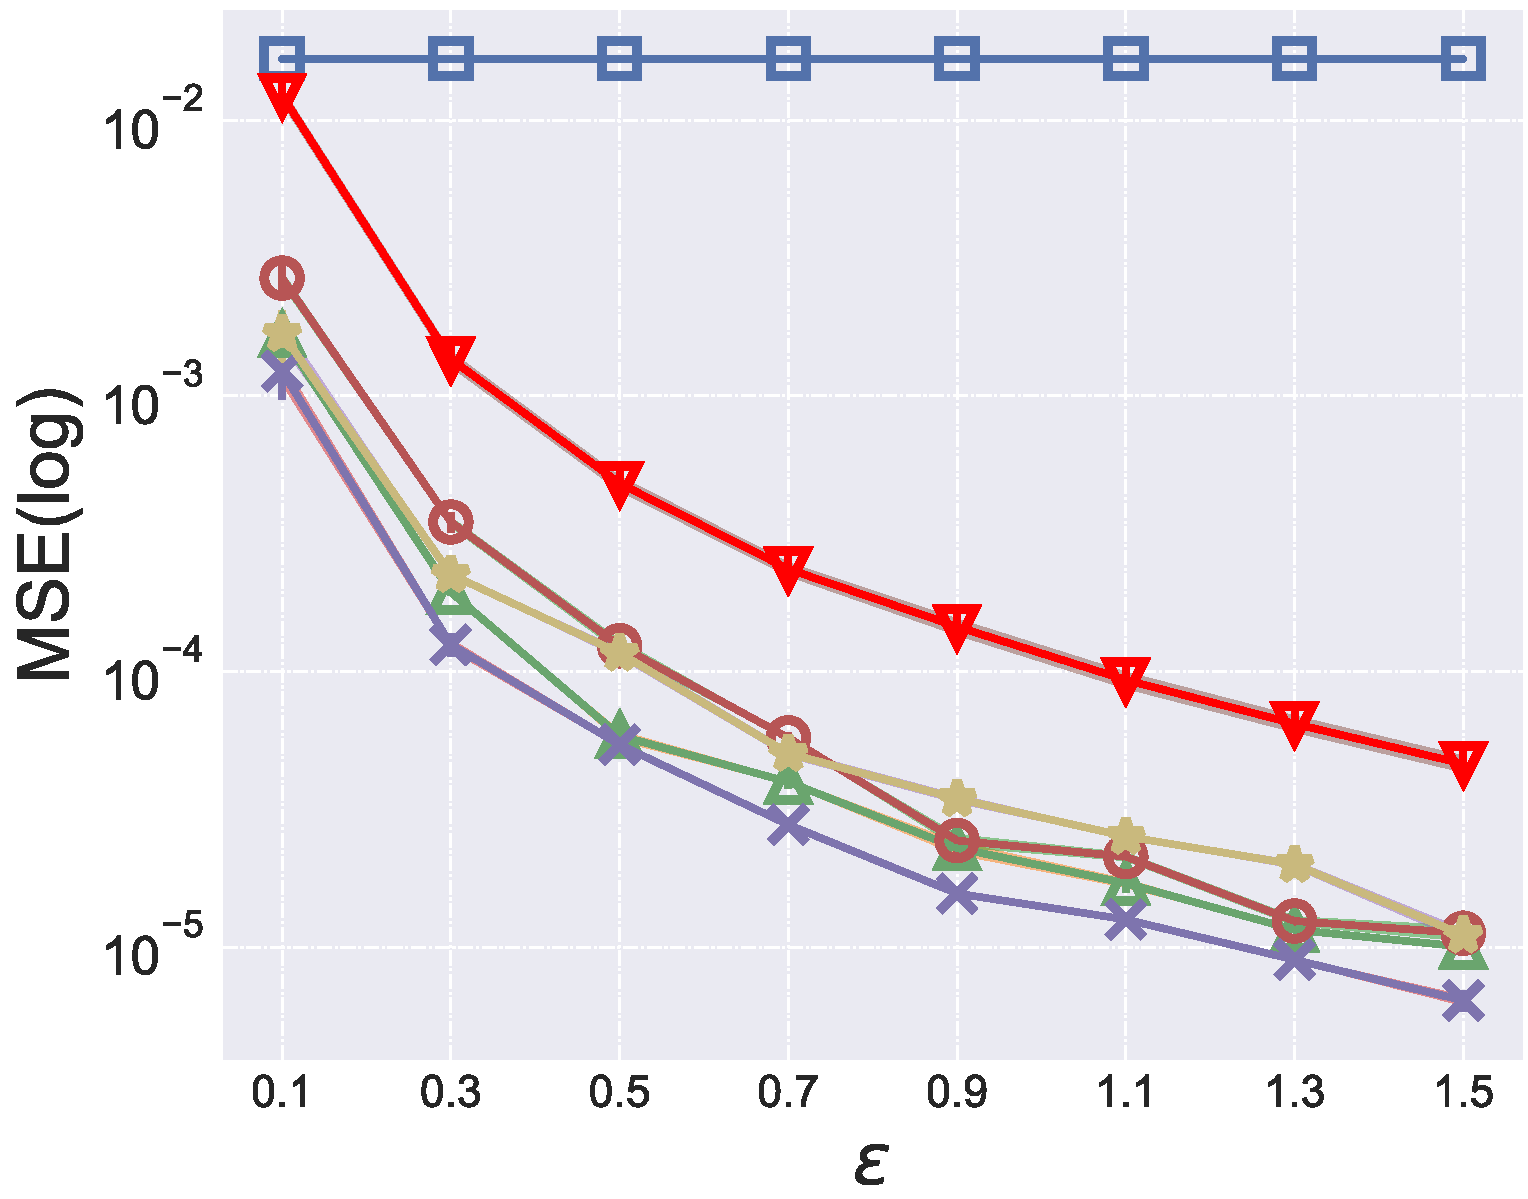
\includegraphics[width=0.23\hsize]{figure/ldp_range_query/figures_experiment_result/0531RandQuery/0404_CI_Rand_ep-Loan-Domain_2_8.pdf.pdf}
    }
    \subfigure[Financial, 512,  vary $\epsilon$]{
    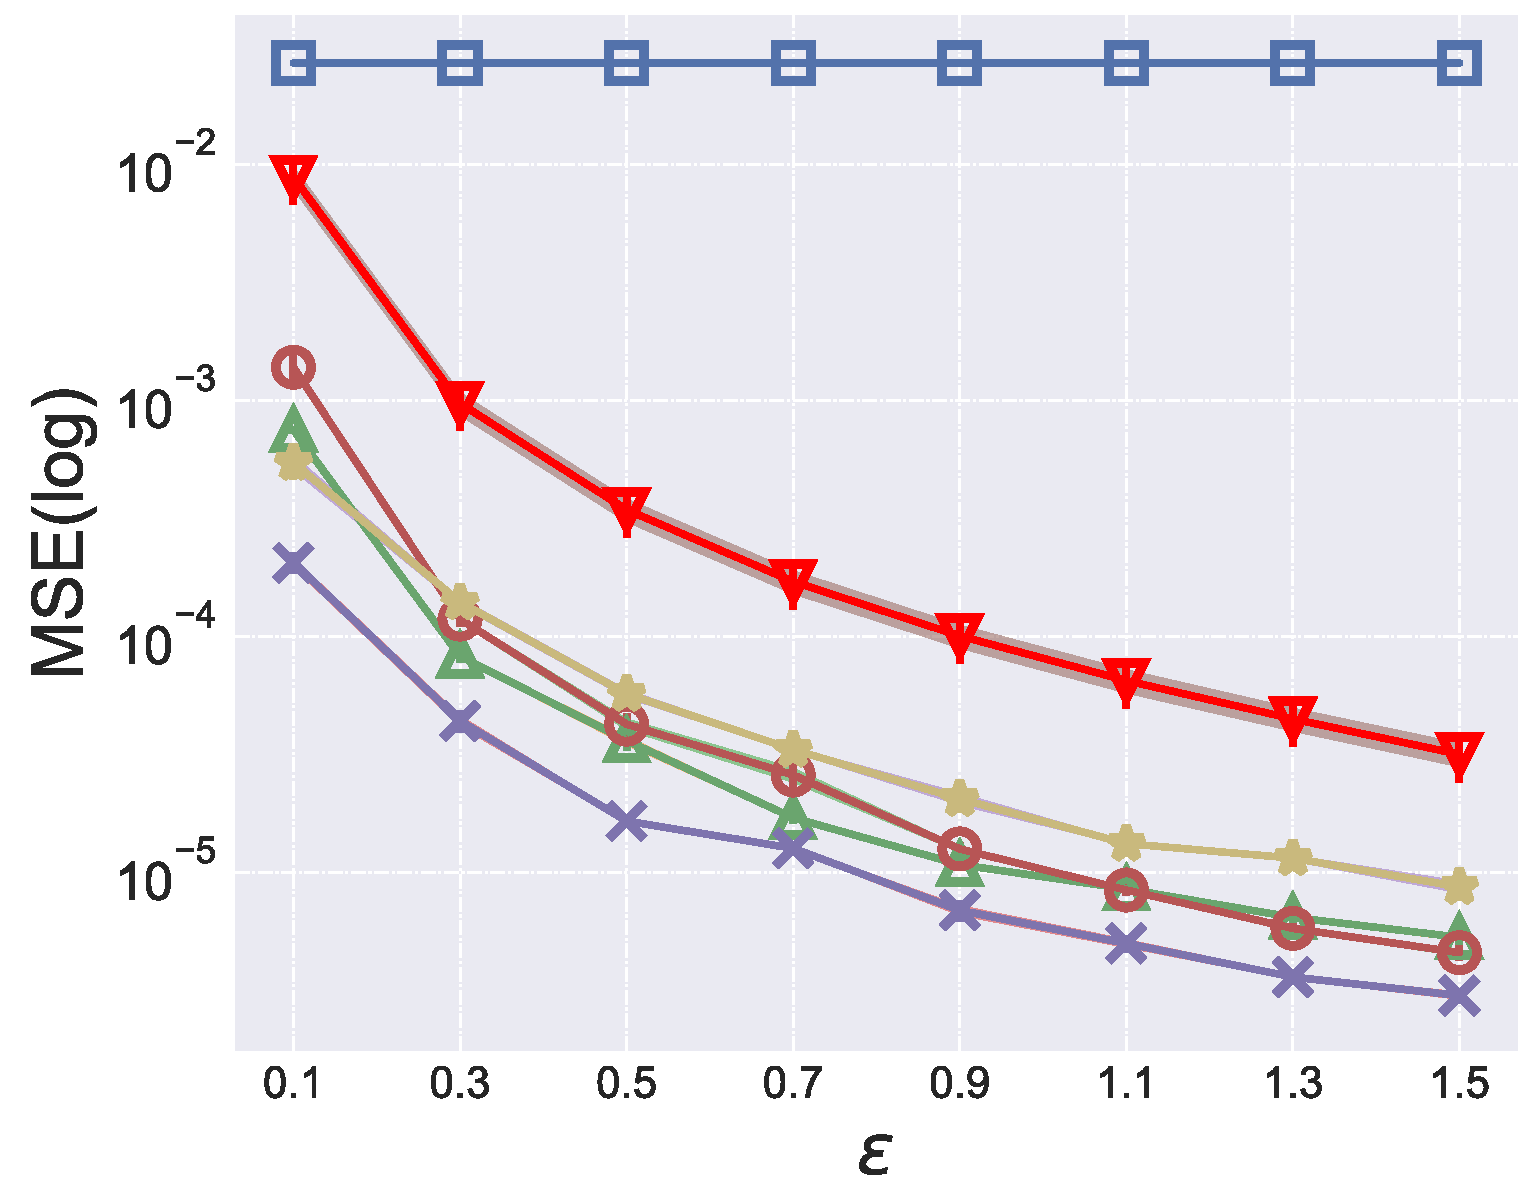
\includegraphics[width=0.23\hsize]{figure/ldp_range_query/figures_experiment_result/0531RandQuery/0404_CI_Rand_ep-Financial-Domain_2_9.pdf.pdf}
    }
    \subfigure[BlackFriday, 1028,  vary $\epsilon$]{
    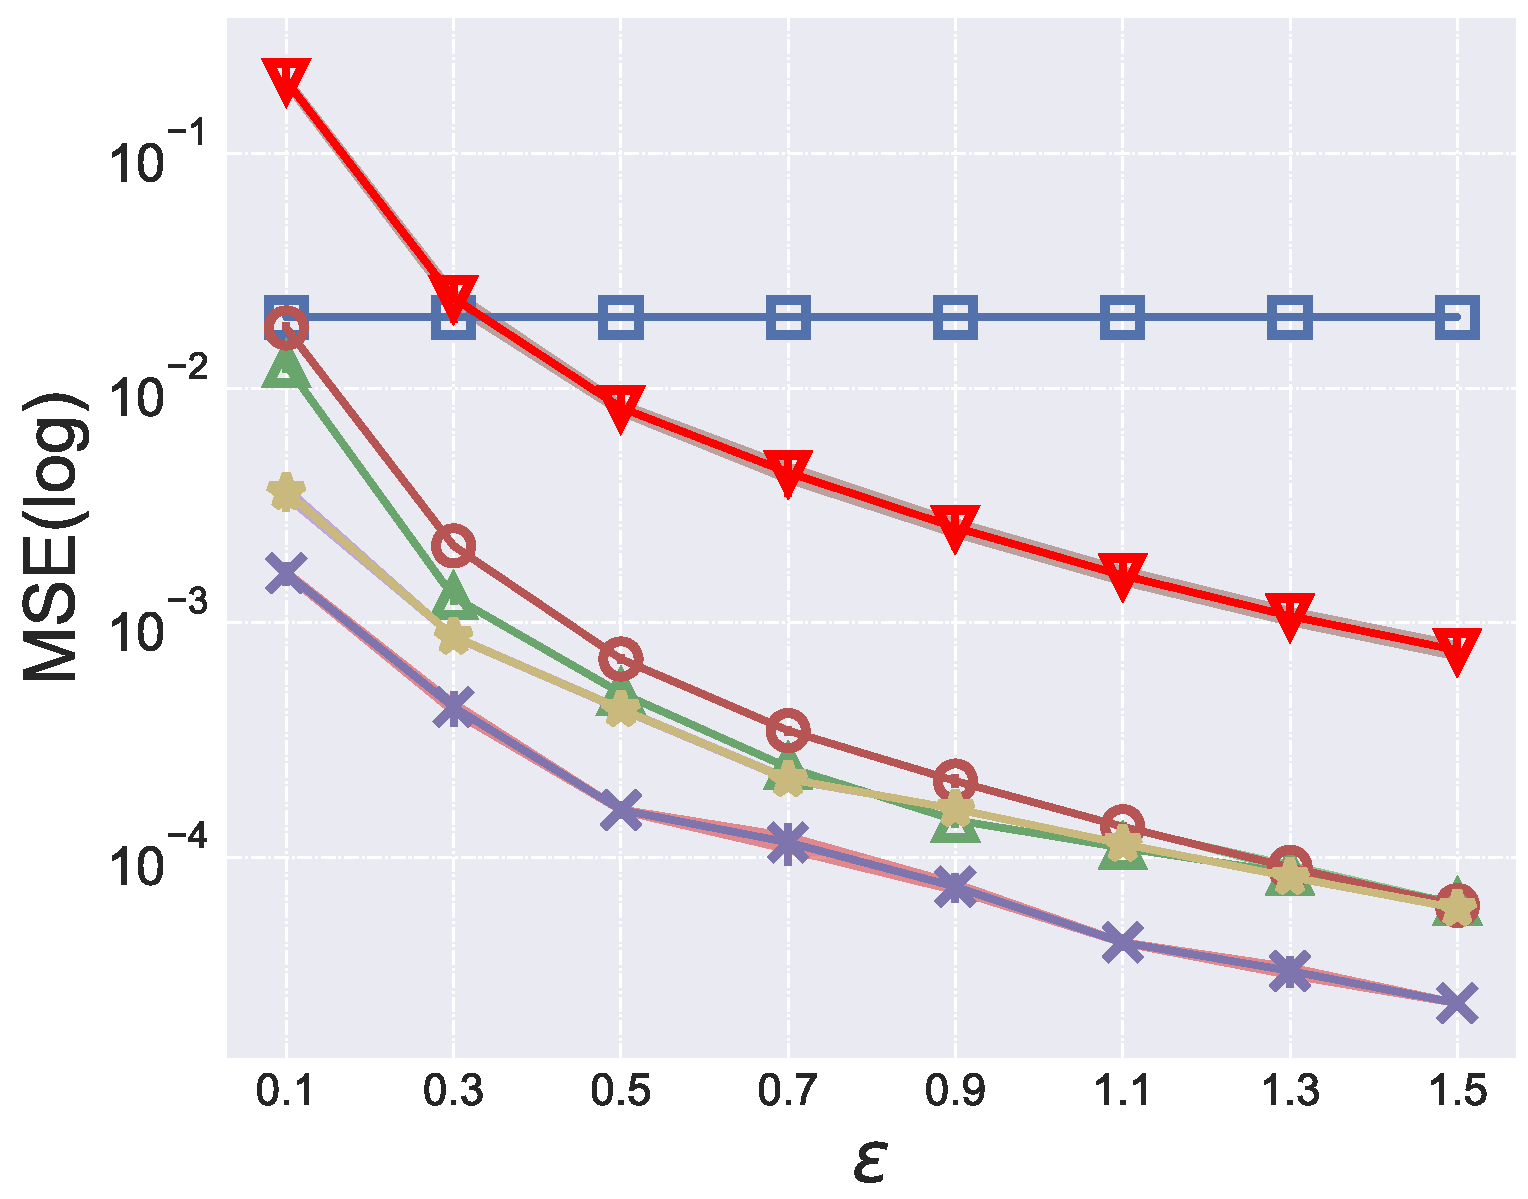
\includegraphics[width=0.23\hsize]{figure/ldp_range_query/figures_experiment_result/0531RandQuery/0404_CI_Rand_ep-BlackFriday-Domain_2_10.pdf.pdf}
    }
    \subfigure[Salaries, 2048,  vary $\epsilon$]{
    \label{overall compare Salaries}
    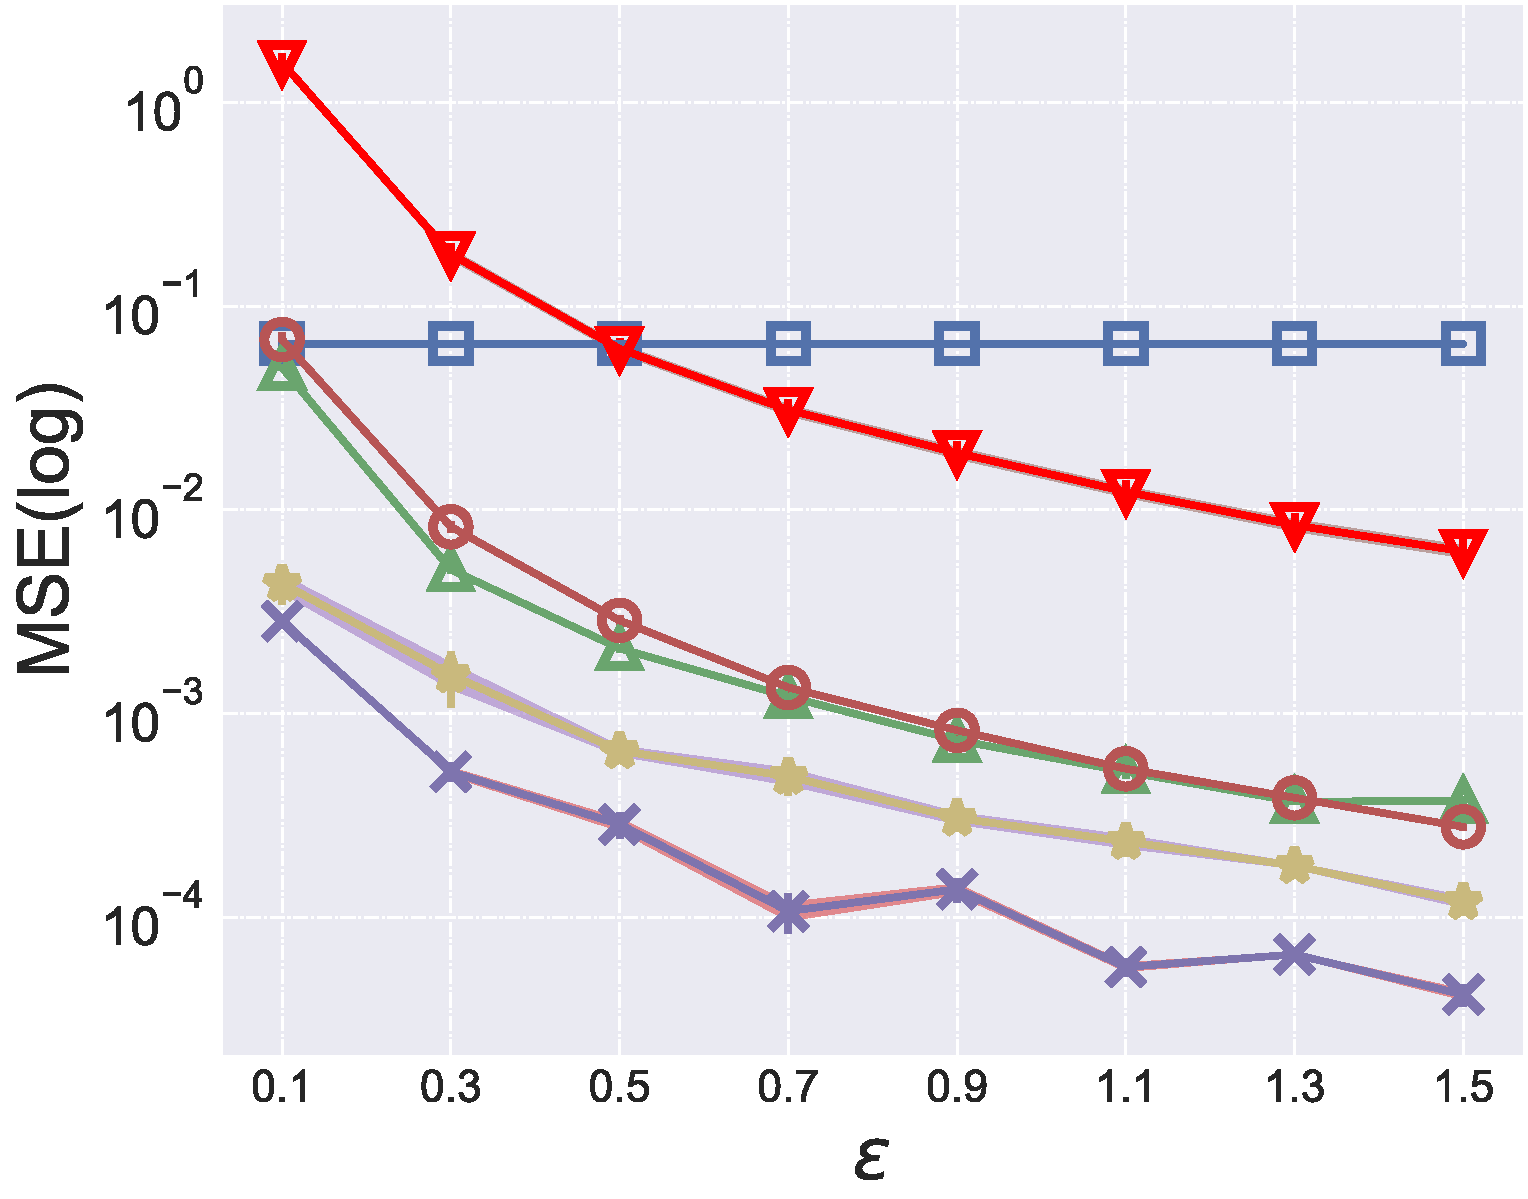
\includegraphics[width=0.23\hsize]{figure/ldp_range_query/figures_experiment_result/0531RandQuery/0404_CI_Rand_ep-Salaries-Domain_2_11.pdf.pdf}
    }
    \\[-0.5ex]
    \subfigure{
    
\includegraphics[width=0.8\hsize]{figure/ldp_range_query/figures_others/comparison_1D_legend6.pdf.pdf} 
    }
    \vspace{-0.2cm}
    \caption{不同方法的MSE,隐私预算从0.1到1.5变化,结果以对数刻度显示。}
    \label{overall compare}
\end{figure*}

我们在多种隐私预算条件下评估\myahead 的有效性。
具体来说,我们将隐私预算$\epsilon$从0.1(表示高隐私保护强度)变化到1.5(表示低隐私保护强度)进行考虑\cite{zhang2018calm, cormode2019answering}。 
\autoref{overall compare}展示了\myahead 与现有文献{\rm\parencite{cormode2019answering, wang2019answering, zhang2018calm}}在一维查询中的MSE比较。
对于每个图,我们在横轴上变化隐私预算$\epsilon$,并在纵轴上展示其相应的MSE。
每个图中的直方图显示20次重复实验MSE的平均值,误差线表示MSE的标准差。

从\autoref{overall compare}中,我们得出以下结论。
1)\myahead 的MSE始终比其他算法小。
回顾\autoref{Selection parameters}中的\autoref{theta setting 2},对于频率值低于阈值的节点,\myahead 采用自适应策略比采用基线策略的对比方法具有更小的总体估计误差。
2)\myahead 在不同数据集上表现不同。对于Salaries数据集,\myahead 在整个隐私预算范围内都比之前的方法显著优越,其中\myahead 的MSE几乎比现有方法小一个数量级。
对于Loan数据集,\myahead 略优于\mydht。
主要是因为这两个数据集具有完全不同的分布特性,
例如Salaries数据集上有更多频率值小于阈值的子域,
而Loan数据集则相对较少,使得\myahead 在这两个数据集上表现不同。


\subsection{二维数据场景}
\begin{figure*}[h!]
    \centering
    \subfigure[\Laplacian, $256^2$, vary $\epsilon$]{\label{fig:Two_Laplace08-Set_10_7-Domain_8_8}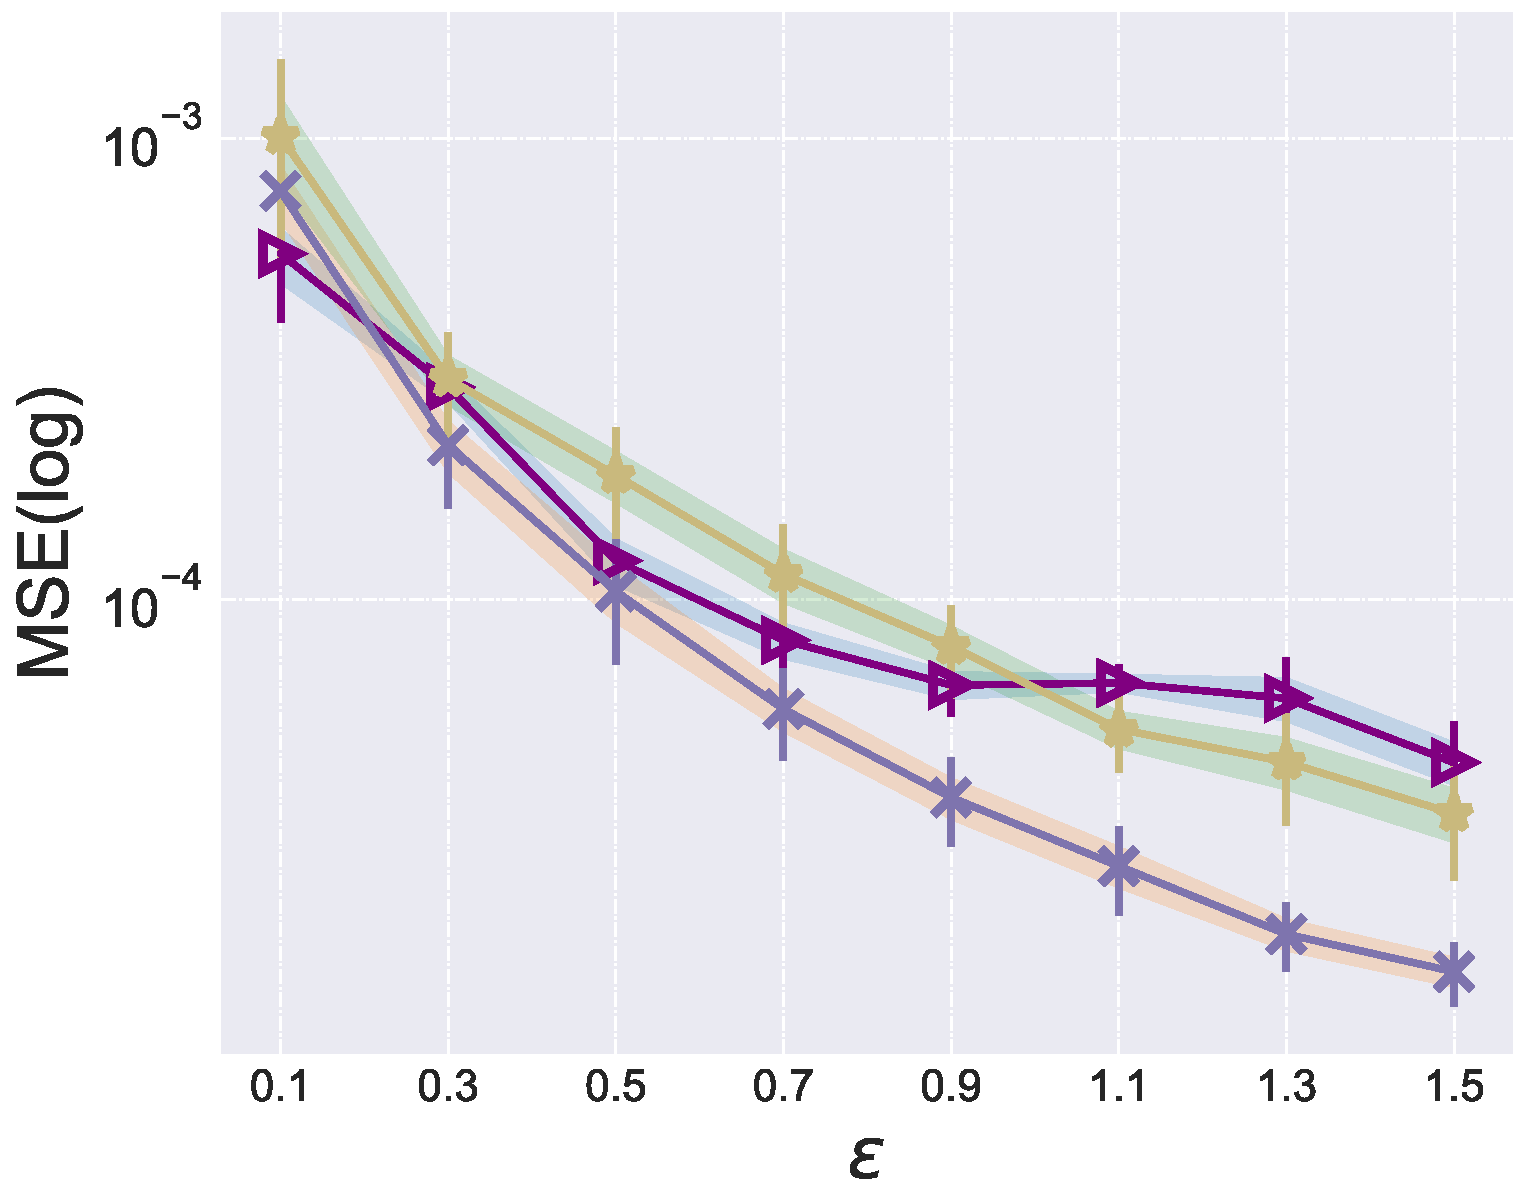
\includegraphics[width=0.24\hsize]{figure/ldp_range_query/figures_experiment_result/overall_result/20210404_CI_Rand_ep-Two_Laplace08-Set_10_7-Domain_8_8.pdf.pdf}}
    \subfigure[\Laplacian, $1024^2$, vary $\epsilon$]{\label{fig:Two_Laplace08-Set_10_7-Domain_10_10}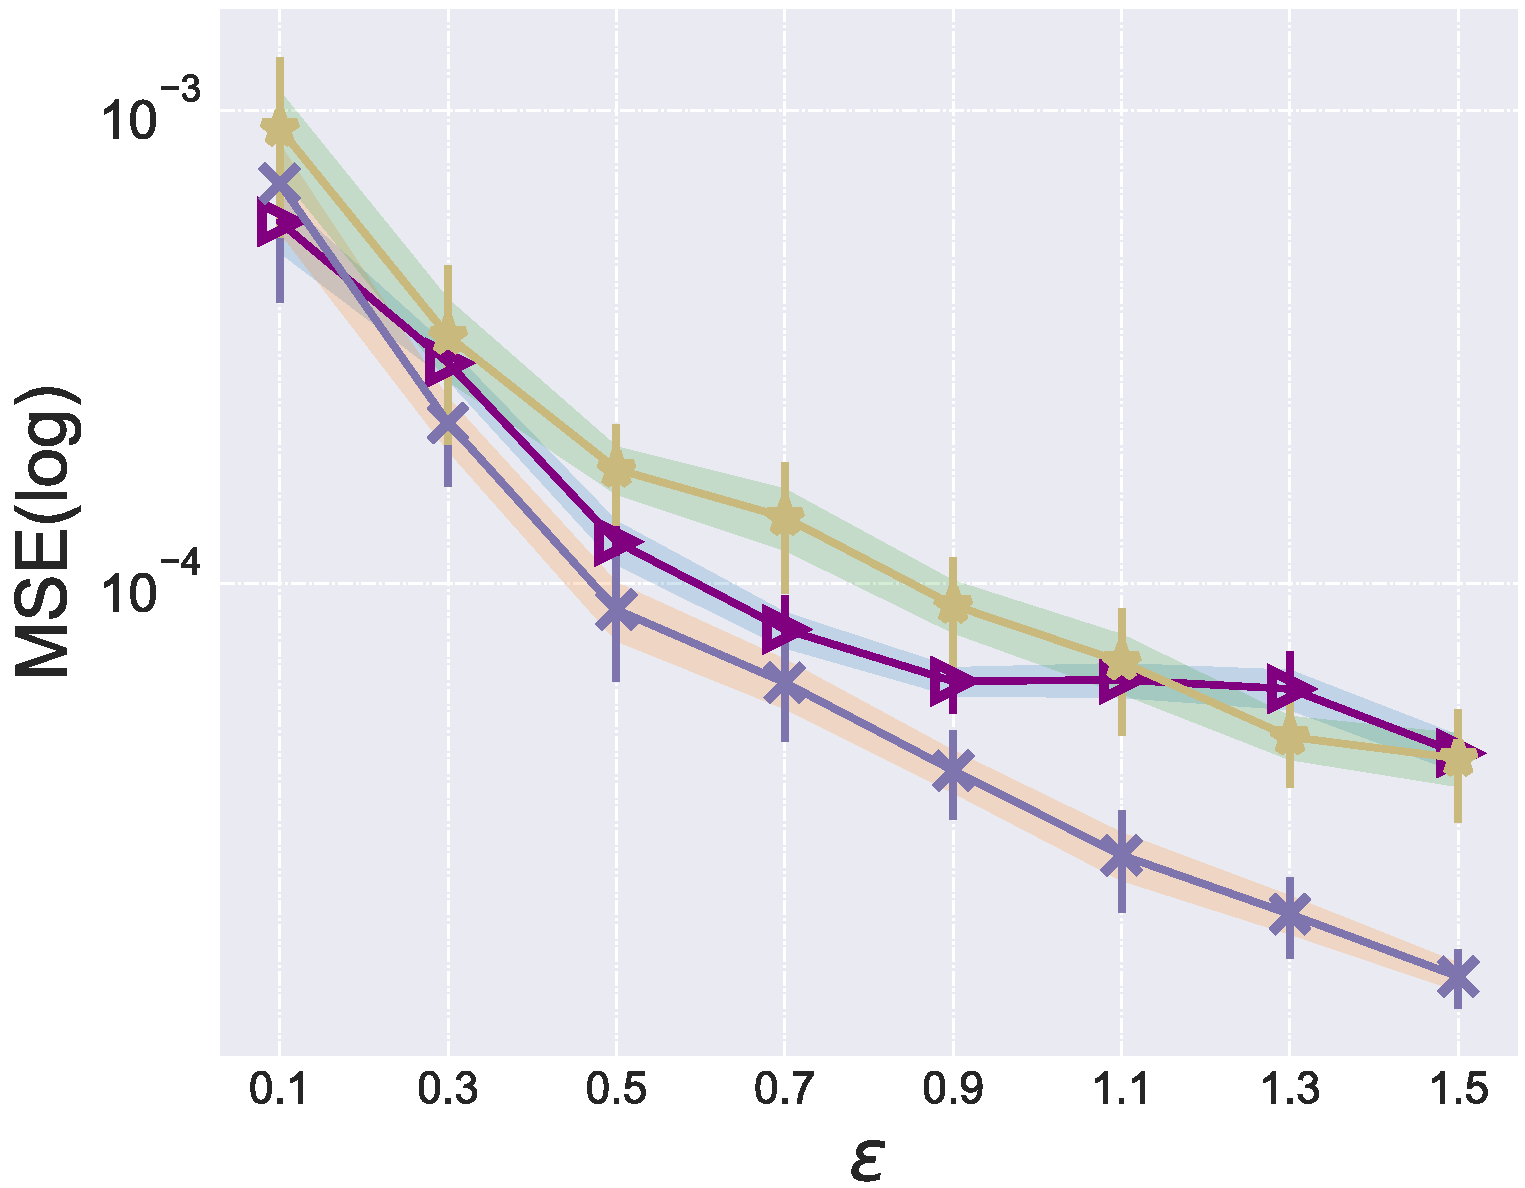
\includegraphics[width=0.24\hsize]{figure/ldp_range_query/figures_experiment_result/overall_result/20210404_CI_Rand_ep-Two_Laplace08-Set_10_7-Domain_10_10.pdf.pdf}}
    \subfigure[\Gaussian, $256^2$, vary $\epsilon$]{\label{fig:Two_Normal08-Set_10_7-Domain_8_8}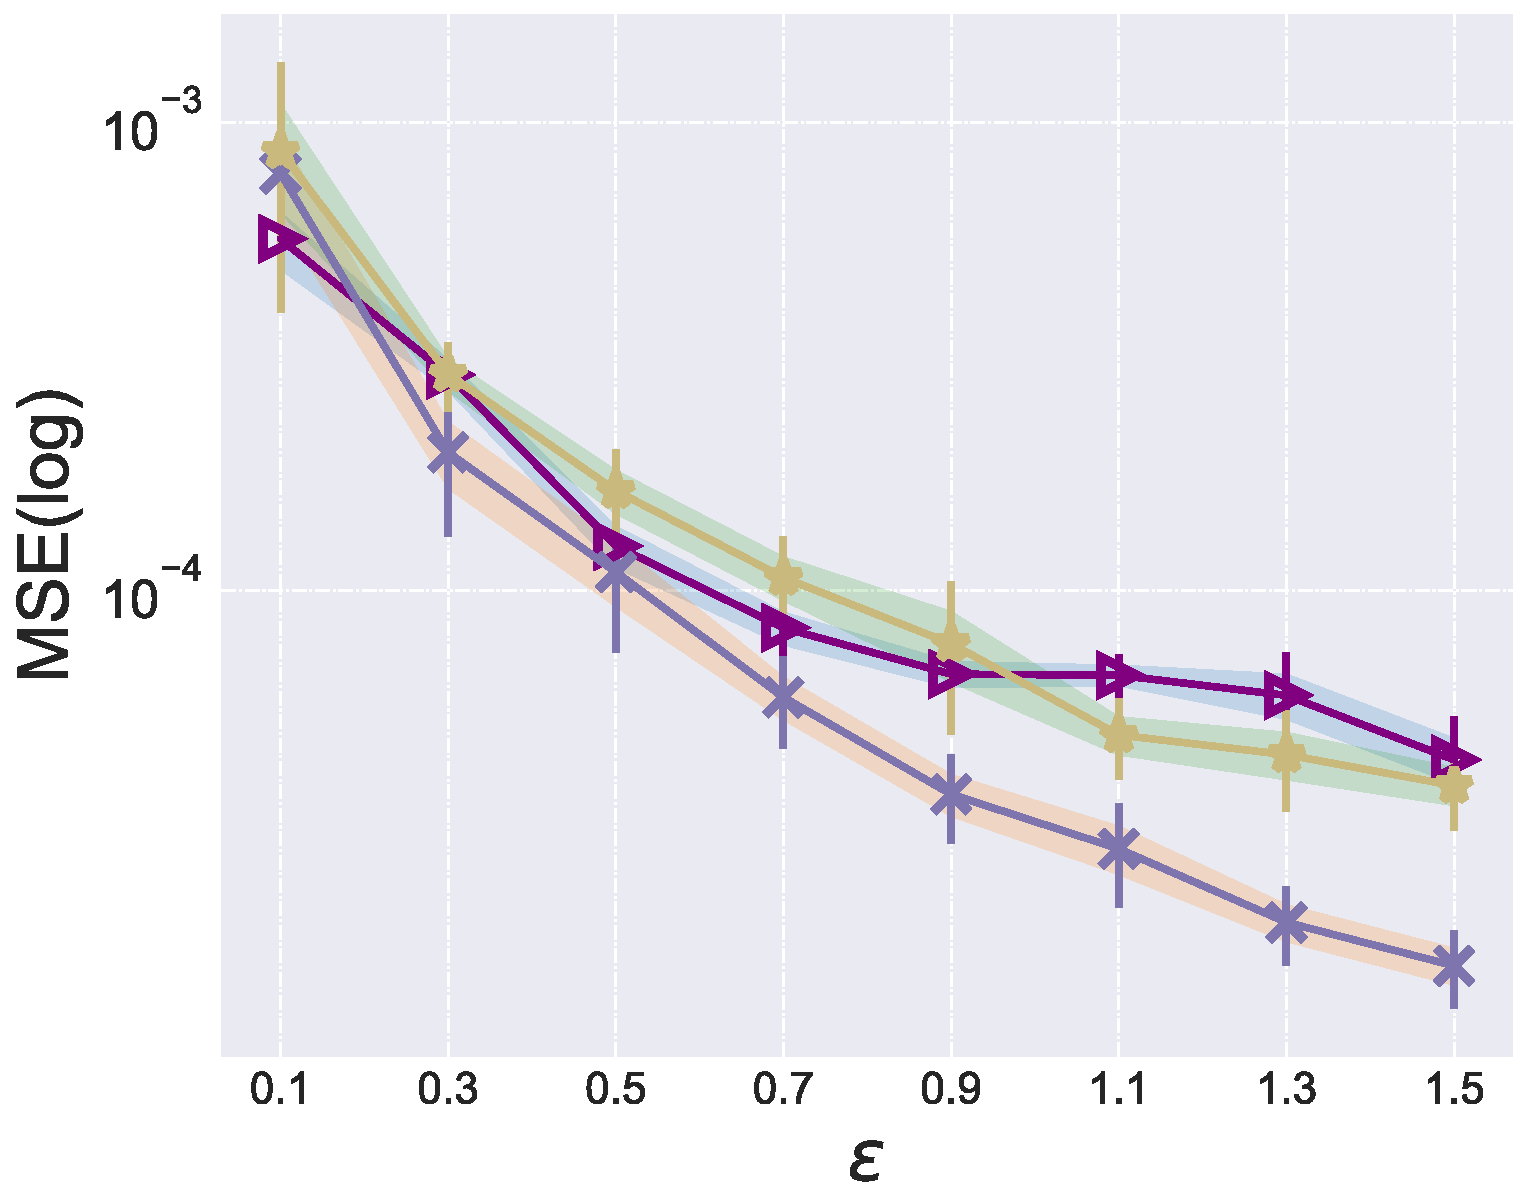
\includegraphics[width=0.24\hsize]{figure/ldp_range_query/figures_experiment_result/overall_result/20210404_CI_Rand_ep-Two_Normal08-Set_10_7-Domain_8_8.pdf.pdf}}
    \subfigure[\Gaussian, $1024^2$, vary $\epsilon$]{\label{fig:Two_Normal08-Set_10_7-Domain_10_10}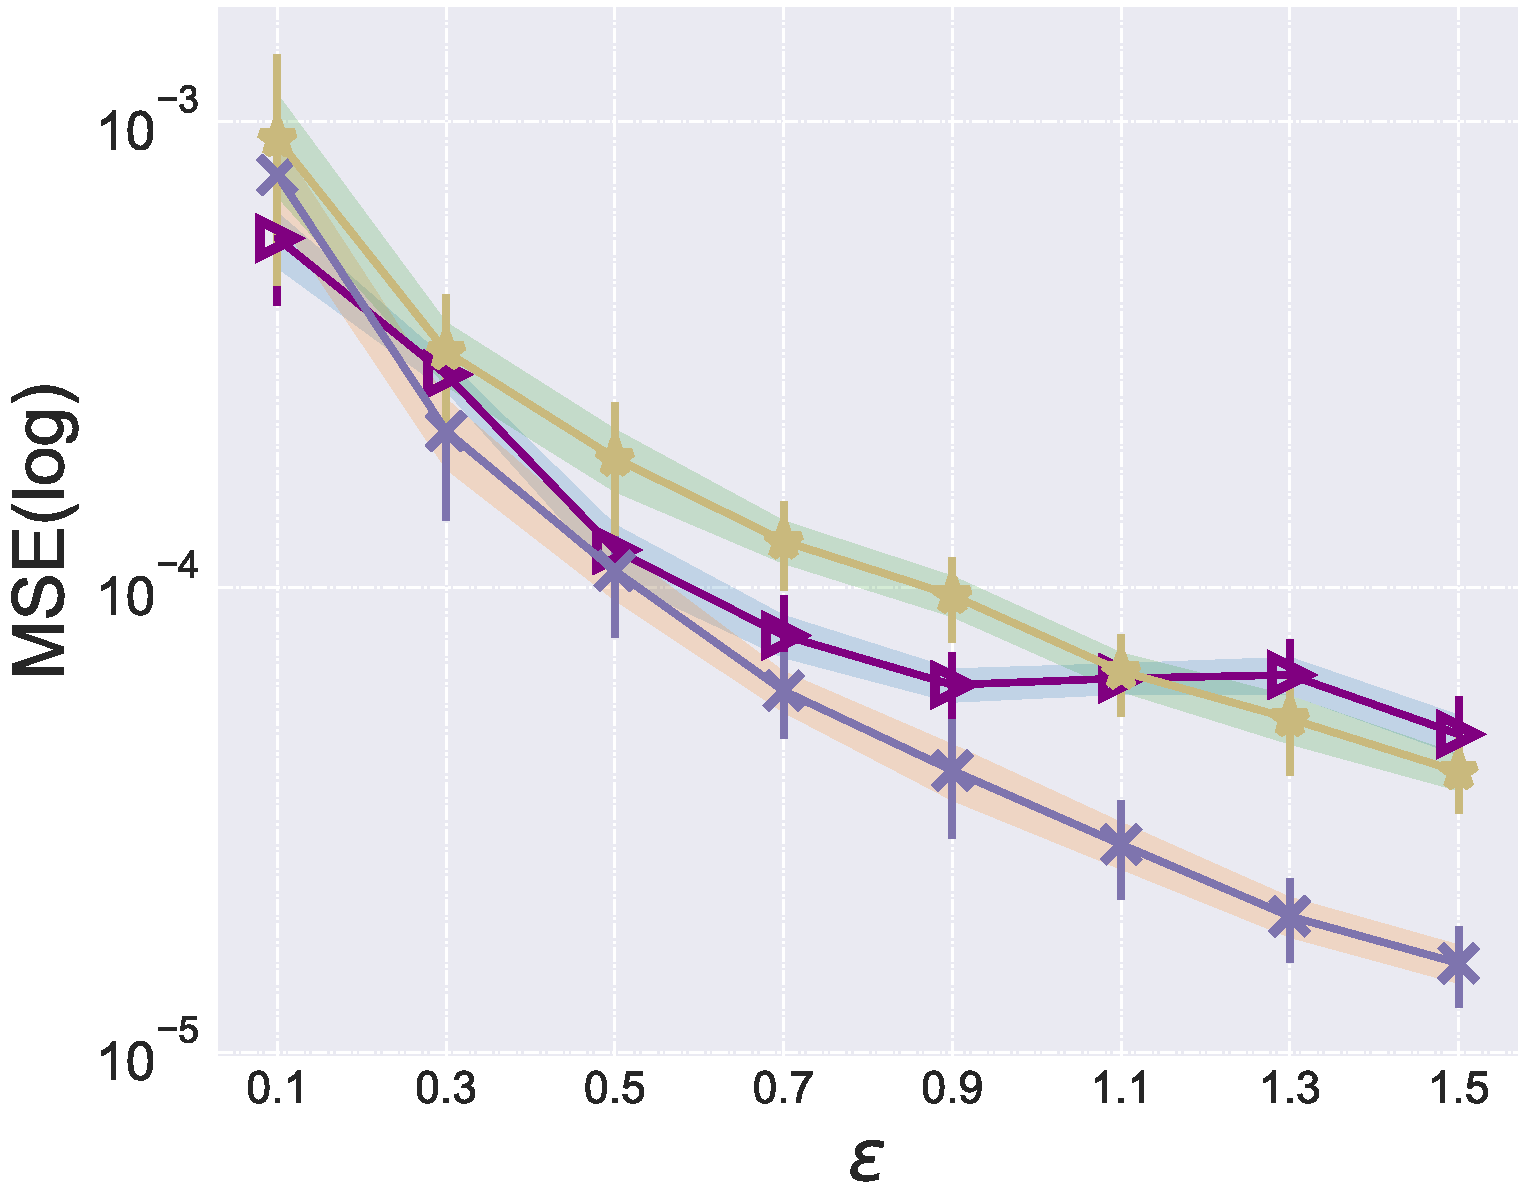
\includegraphics[width=0.24\hsize]{figure/ldp_range_query/figures_experiment_result/overall_result/20210404_CI_Rand_ep-Two_Normal08-Set_10_7-Domain_10_10.pdf.pdf}}
    \\[-0.5ex]
    \subfigure{
\includegraphics[width=0.4\textwidth]{figure/ldp_range_query/figures_others/comparison_2D_legend.pdf.pdf}} 
    \vspace{-0.2cm}
    \caption{
        % Comparison of different methods on \Laplacian and \Gaussian datasets under various privacy budgets. We only plot the methods that are scalable in each setting. \myHDG is a baseline method. The results are shown in log scale.
        基于\Laplacian 和 \Gaussian 数据集,我们比较了\myahead 和现有方法在不同隐私预算下的性能,结果以对数刻度显示。其中,\myHDG 是基准方法。}
    % \vspace{-0.5cm}
    \label{2-dim overall compare}
\end{figure*}

\begin{figure*}[h!]
    \centering
    \subfigure[\Laplacian, $256^2$, vary $r$]{\label{fig:Two_Laplace08-Set_10_7-Domain_8_8}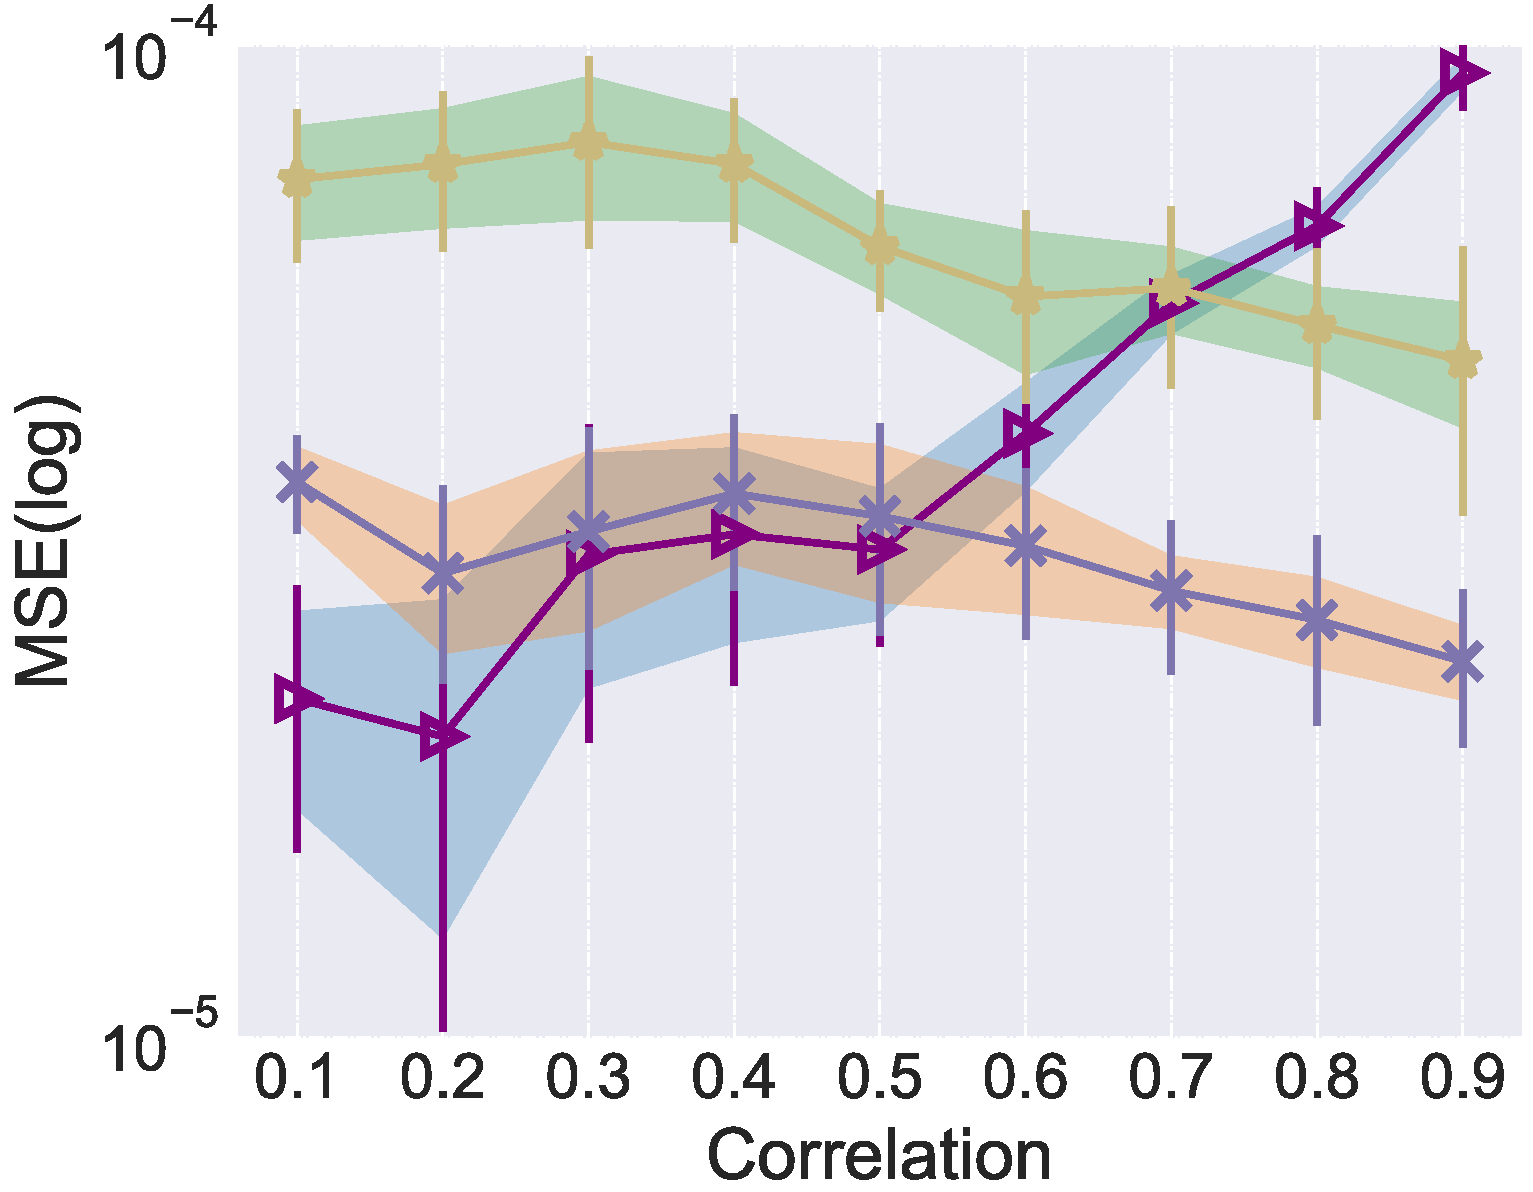
\includegraphics[width=0.24\hsize]{figure/ldp_range_query/figures_experiment_result/overall_result/20210404Correlation-Two_Laplace-Set_10_7-Domain_8_8.pdf.pdf}}
    \subfigure[\Laplacian, $1024^2$, vary $r$]{\label{fig:Two_Laplace09-Set_10_7-Domain_8_8}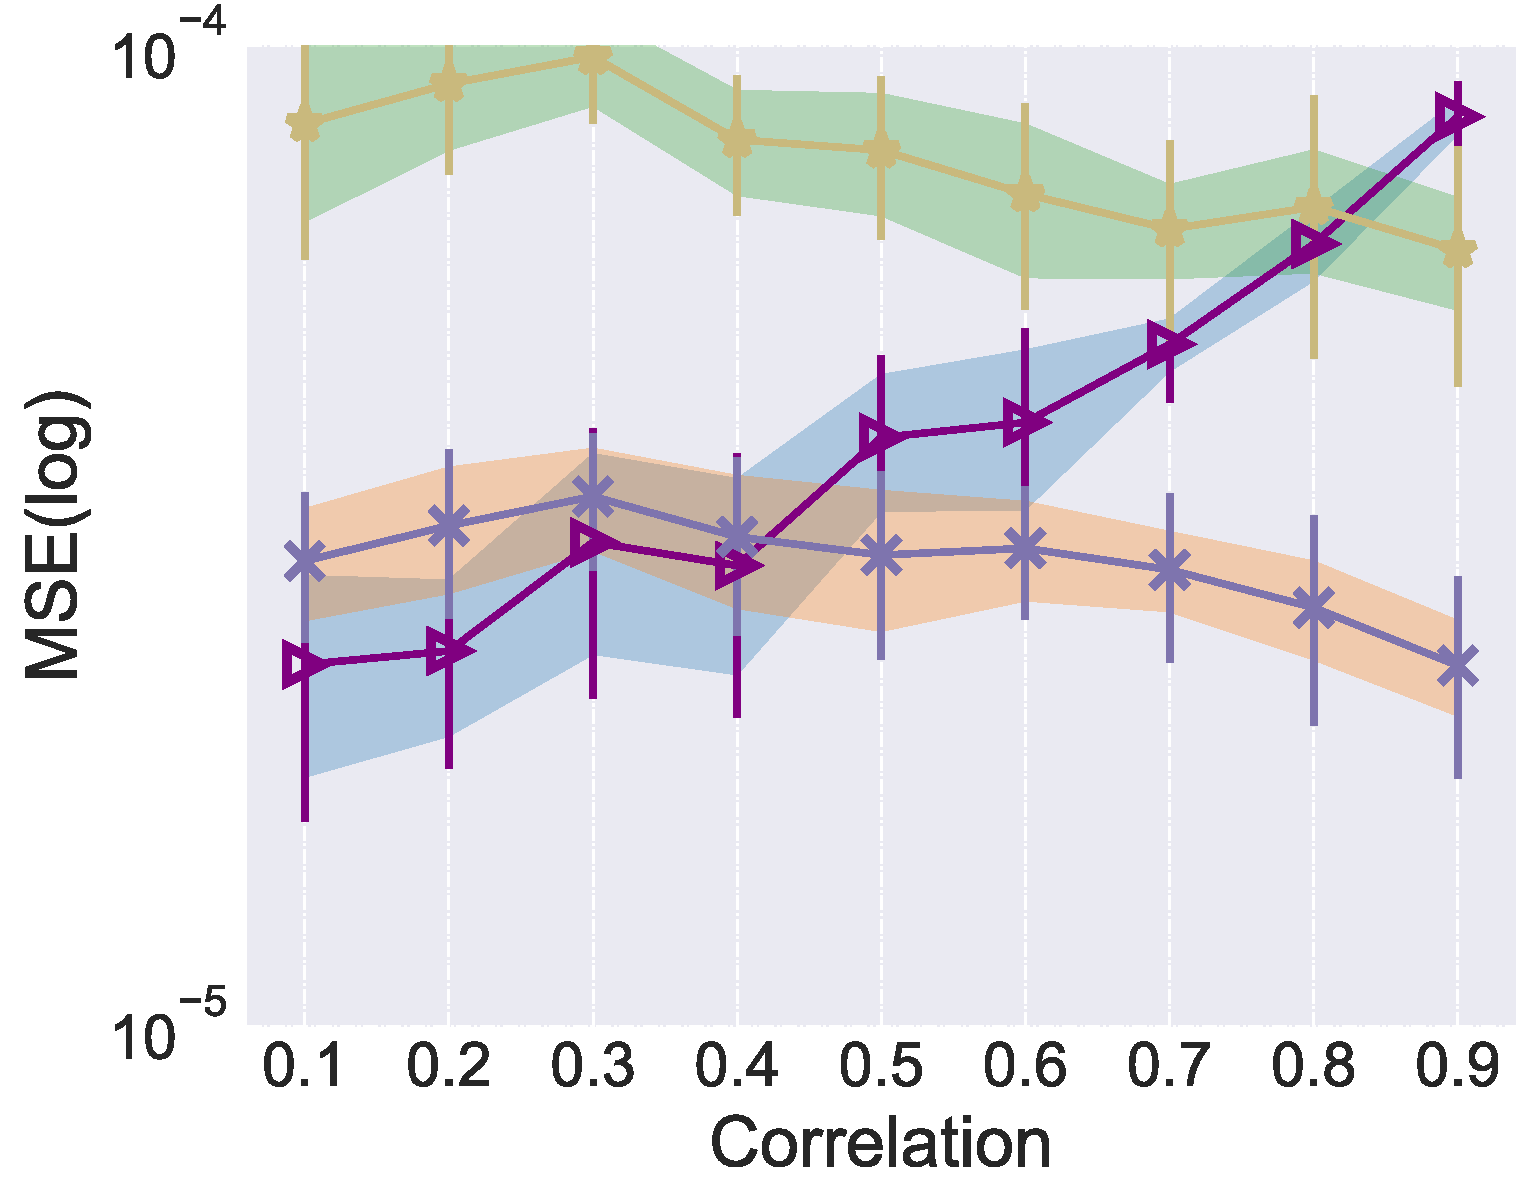
\includegraphics[width=0.24\hsize]{figure/ldp_range_query/figures_experiment_result/overall_result/20210404Correlation-Two_Laplace-Set_10_7-Domain_10_10.pdf.pdf}}
    \subfigure[\Gaussian, $256^2$, vary $r$]{\label{fig:Two_Laplace08-Set_10_7-Domain_10_10}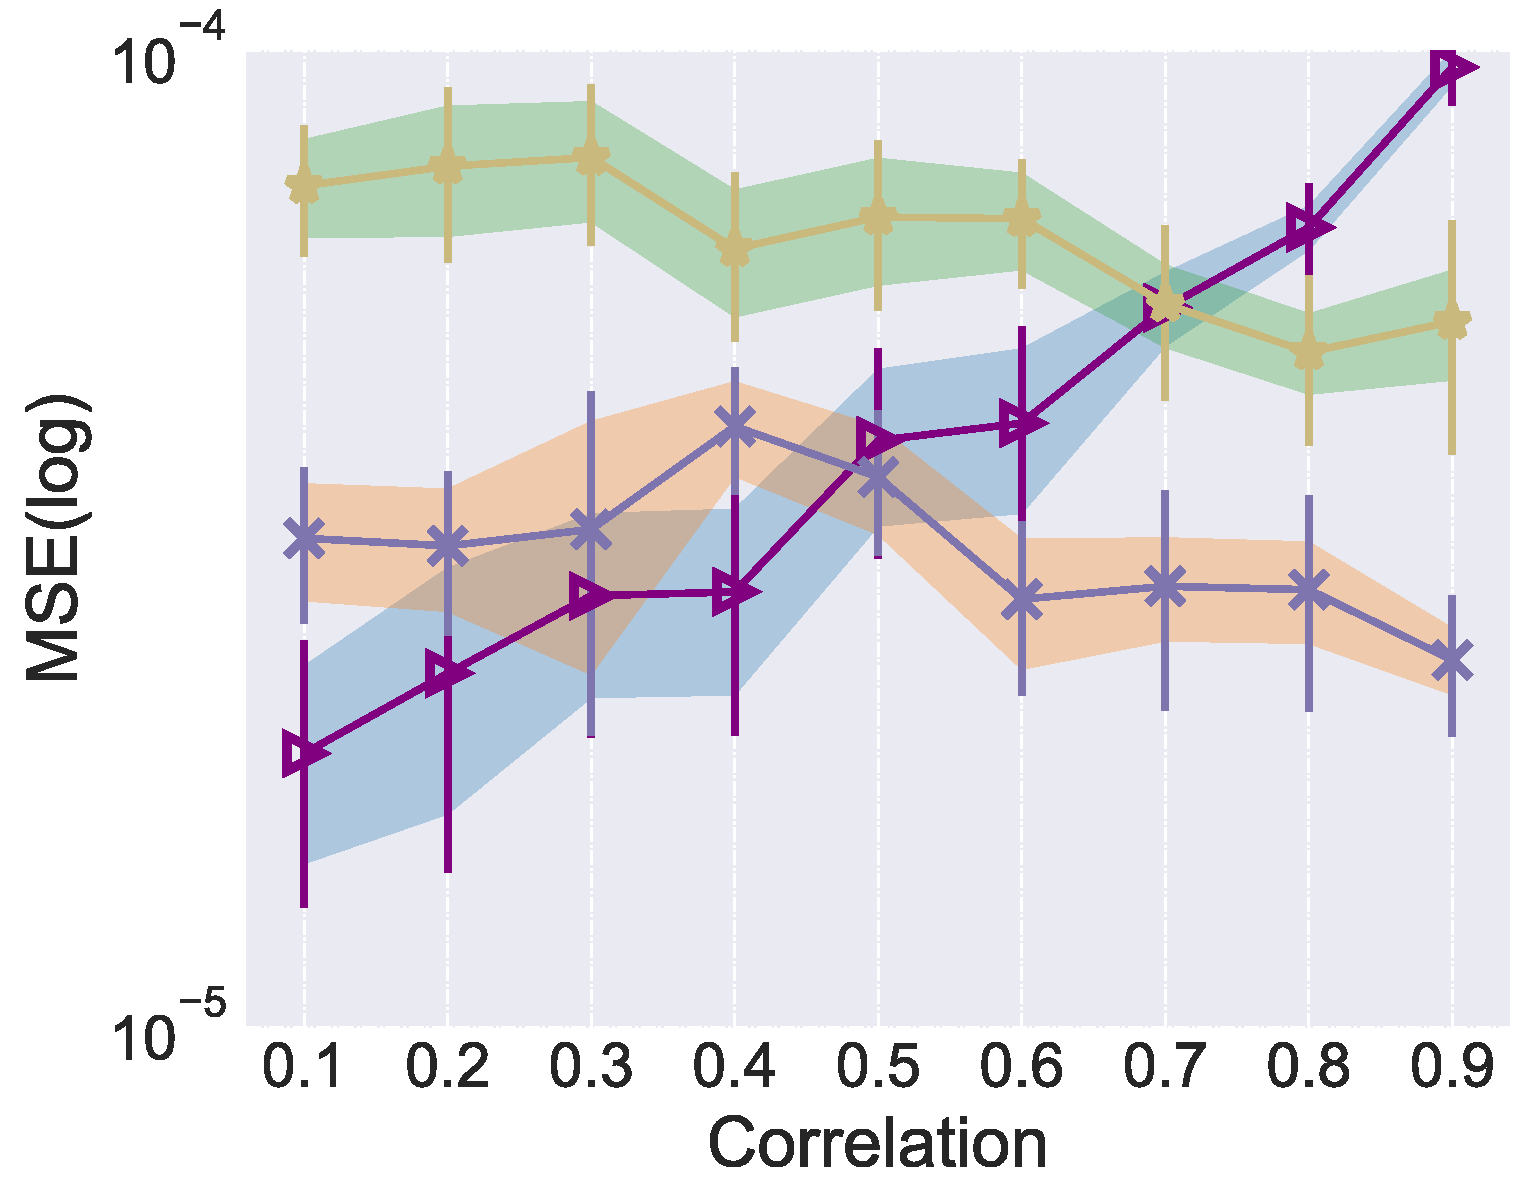
\includegraphics[width=0.24\hsize]{figure/ldp_range_query/figures_experiment_result/overall_result/20210404Correlation-Two_Normal-Set_10_7-Domain_8_8.pdf.pdf}}
    \subfigure[\Gaussian, $1024^2$, vary $r$]{\label{fig:Two_Laplace09-Set_10_7-Domain_10_10}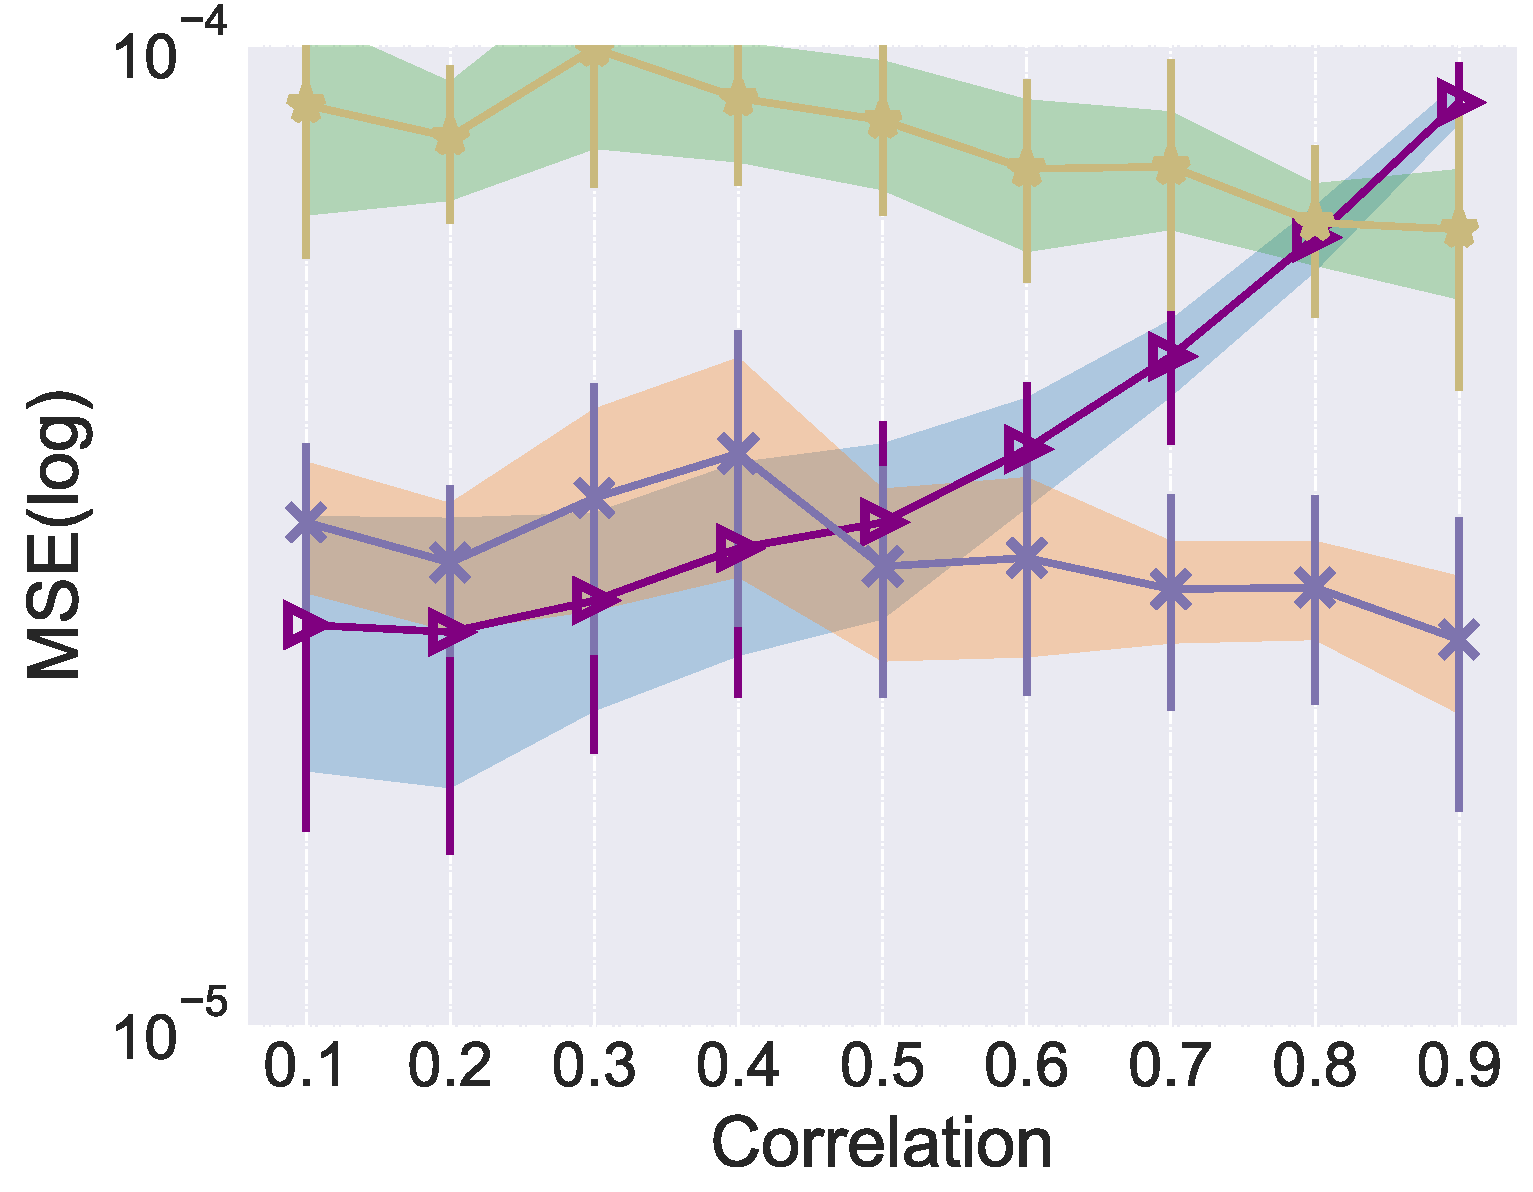
\includegraphics[width=0.24\hsize]{figure/ldp_range_query/figures_experiment_result/overall_result/20210404Correlation-Two_Normal-Set_10_7-Domain_10_10.pdf.pdf}}
    \\[-0.5ex]
    \subfigure{
\includegraphics[width=0.4\textwidth]{figure/ldp_range_query/figures_others/comparison_2D_legend.pdf.pdf}}  
    \vspace{-0.2cm}
    \caption{基于\Laplacian 和 \Gaussian 数据集,我们比较了\myahead 和现有方法在不同属性相关性下的性能,结果以对数刻度显示。其中,\myHDG 是基准方法。}
    % \vspace{-0.5cm}
    \label{2-dim correlation}
\end{figure*}

\mypara{不同隐私预算下的算法查询精度}
我们评估了在二维查询下不同隐私预算对算法性能的影响。
% 在这里,我们专注于合成数据集,因为它们可以反映算法在标准分布上的性能,并有助于调整数据集参数。
每个数据集包含$10^7$条记录,分别从二维\Laplacian 分布和\Gaussian 分布中进行采样,
其中数据域大小分别为$256 \times 256$和$1024 \times 1024$。

\autoref{2-dim overall compare}展示了在二维\Laplacian 分布和\Gaussian 分布的结果。
我们采用与\cite{yang2020answering}相同的相关系数$r=0.8$。
由于\myuni 和\mycalm 的MSE超出了图表范围,因此我们省略了它们的结果。
根据结果,我们有以下观察结果。
1)在不同的隐私预算设置下,\myahead 表现优于\myHDG 。
\myHDG 利用粗粒度的二维网格对二维数据域进行划分,并刻画两个属性之间的相关信息。
当数据域大小为$1024 \times 1024$时,\myHDG 的最精细粒度是$8 \times 8$。
采用粗粒度的网格进行划分会导致数据相关性信息丢失。
相比之下,\myahead 针对具有不同频率值的子域使用多粒度分解方式。
对于一个用户数据集中分布的子域,\myahead 采用细粒度分解,以更准确地提取数据相关性。
2)\myahead 对于不同数据域大小具有鲁棒性。
一方面,更大的数据域意味着需要将用户划分为更多的组。
例如,对于$256 \times 256$的数据域,\myahead 将用户划分为8组。
而对于$1024 \times 1024$的数据域,\myahead 将用户划分为10组。
对于更大的数据域,每个组中的用户数量较少,这将增加频率值中添加的噪声。
另一方面,频率小于阈值的子域不会被进一步划分。
我们使用多个用户组的上传数据估计这些子域的频率值。
在后向处理中进行加权平均处理后,这些子域的噪声误差将变为原始噪声误差的$\frac{1}{\beta}$,其中$\beta$是估计次数。
% 通过比较\autoref{2-dim overall compare}中的两个相邻子图,阈值设置的影响比域大小变化的影响更大。因此,\myahead的MSE几乎不随不同域大小变化而变化,我们选择不同的域大小来进一步验证这一事实,详见\autoref{Impact of Domain Size}。

\mypara{不同属性相关性下的算法查询精度}
我们在\autoref{2-dim correlation}中展示了在不同属性相关性下查询误差。
在每个子图中,我们使用固定的隐私预算$\epsilon=1.1$,并将相关系数$r$从0.1(弱相关)变化到0.9(强相关)。
基于实验结果,我们总结出以下结论。
1)\myahead 的MSE几乎不随属性相关性而改变。
\myahead 同时分解了两个维度,因此更好地保护了数据的相关性。
2)\myHDG 的数据效用会随着属性相关性的增加而降低,特别是在属性相关性较强的情况下。
\myHDG 结合了更细粒度的一维网格来估计频率分布。
如果两个属性之间的相关性较弱,细粒度的一维网格可以弥补粗粒度的二维网格的精度不足的缺陷。
当属性之间的相关性较强时,缺少属性相关性信息的一维网格可能会对查询精度造成负面影响。
% 有趣的是,相关系数$r=0.5$似乎是\myHDG 和\myahead 的交点,这可能引导聚合器根据属性的相关性选择更好的算法。
% 对于高维场景,我们还在\autoref{Impact of Attribute Correlation}中评估了不同属性相关性对查询误差的影响,其中\myahead 的反应与二维场景类似。

\subsection{高维数据场景}
\label{Effectiveness of ahead for high-dimensional Range Query}
\begin{figure*}[h!]
    \centering
    \subfigure[\Laplacian~(3), $10^6$, vary $\epsilon$]{\label{fig:Three_Laplace08-Set_10_6-Domain_6_6_6}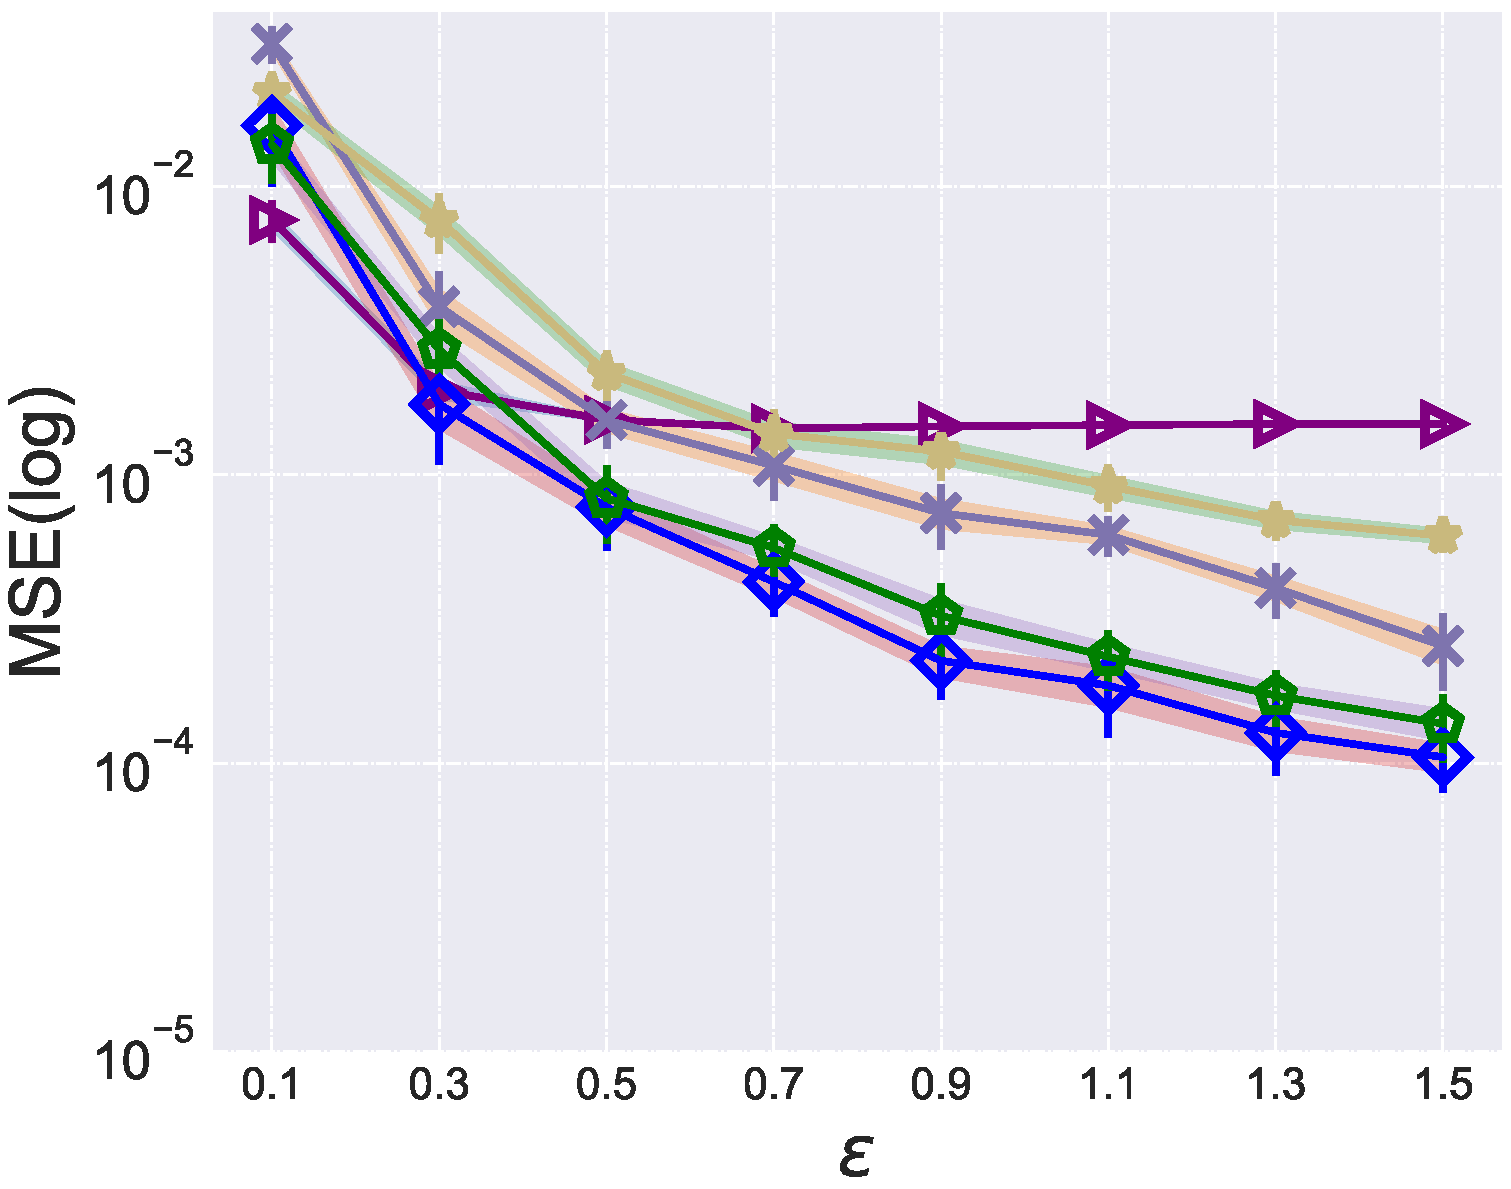
\includegraphics[width=0.24\hsize]{figure/ldp_range_query/figures_experiment_result/overall_result/0406_CI_Rand_ep-Three_Laplace08-Set_10_6-Domain_6_6_6.pdf.pdf}}
    \subfigure[\Laplacian~(3), $10^7$, vary $\epsilon$]{\label{fig:Three_Laplace08-Set_10_7-Domain_6_6_6}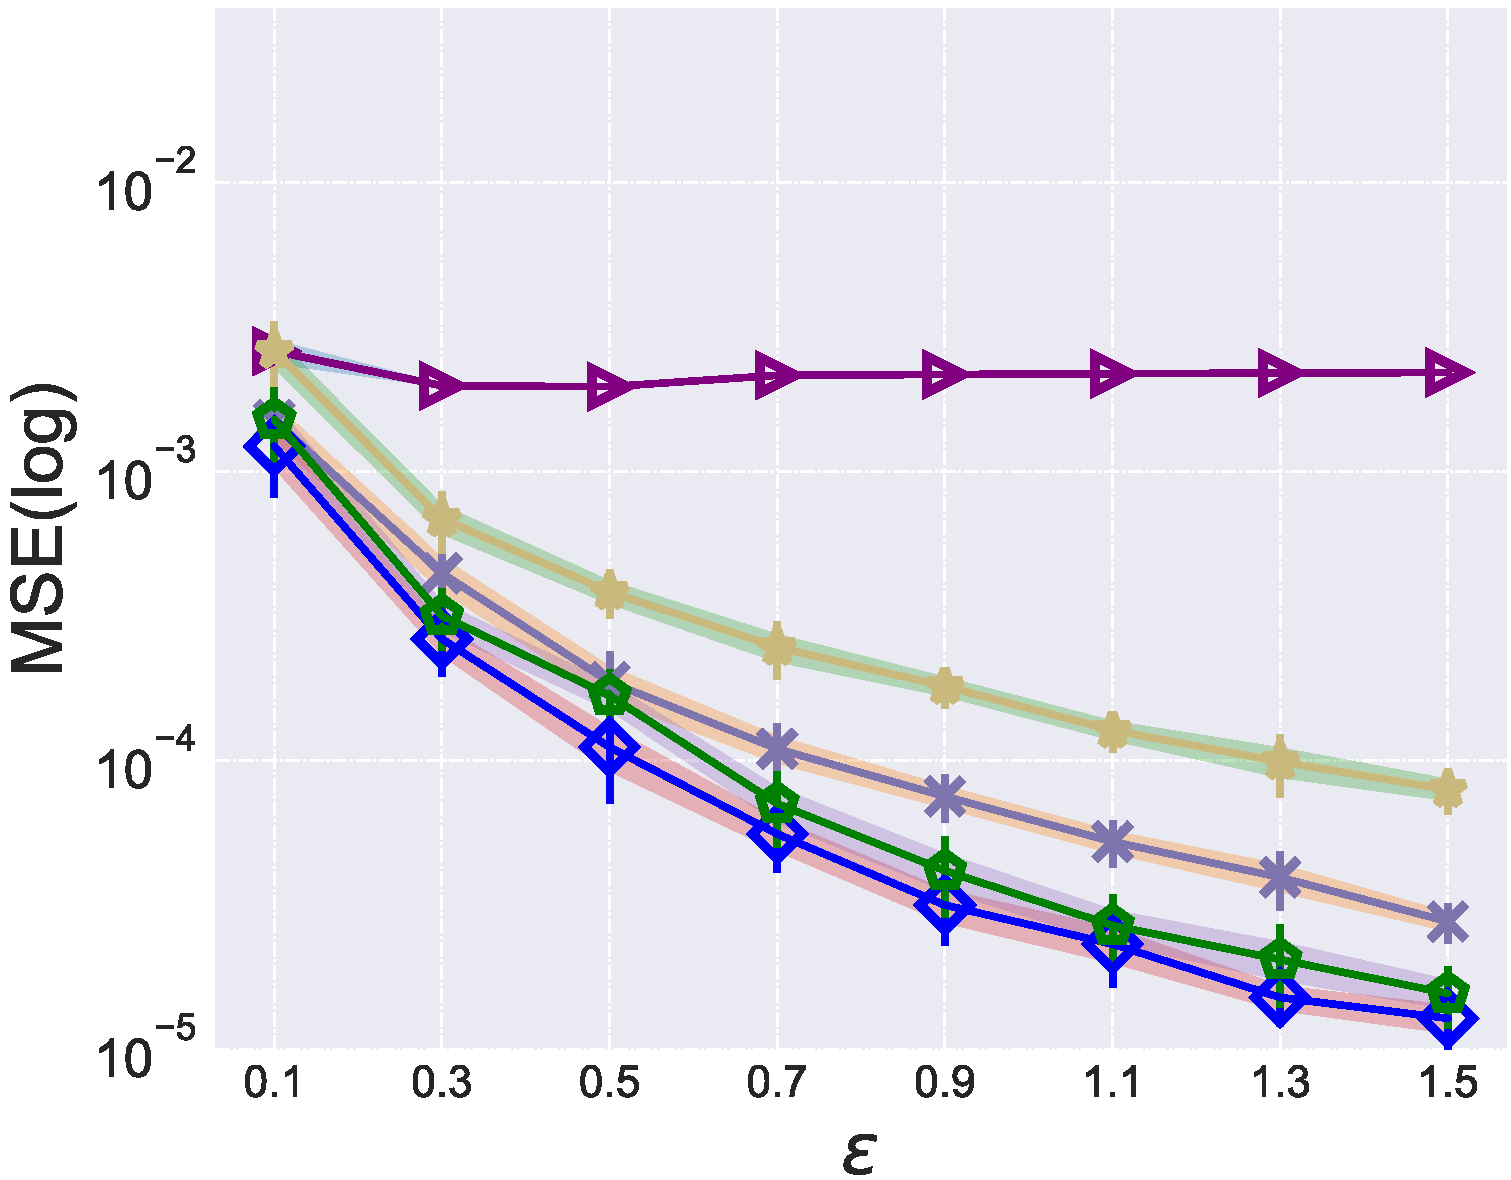
\includegraphics[width=0.24\hsize]{figure/ldp_range_query/figures_experiment_result/overall_result/0406_CI_Rand_ep-Three_Laplace08-Set_10_7-Domain_6_6_6.pdf.pdf}}
    \subfigure[\Gaussian~(3), $10^6$, vary $\epsilon$]{\label{fig:Three_Normal08-Set_10_6-Domain_6_6_6}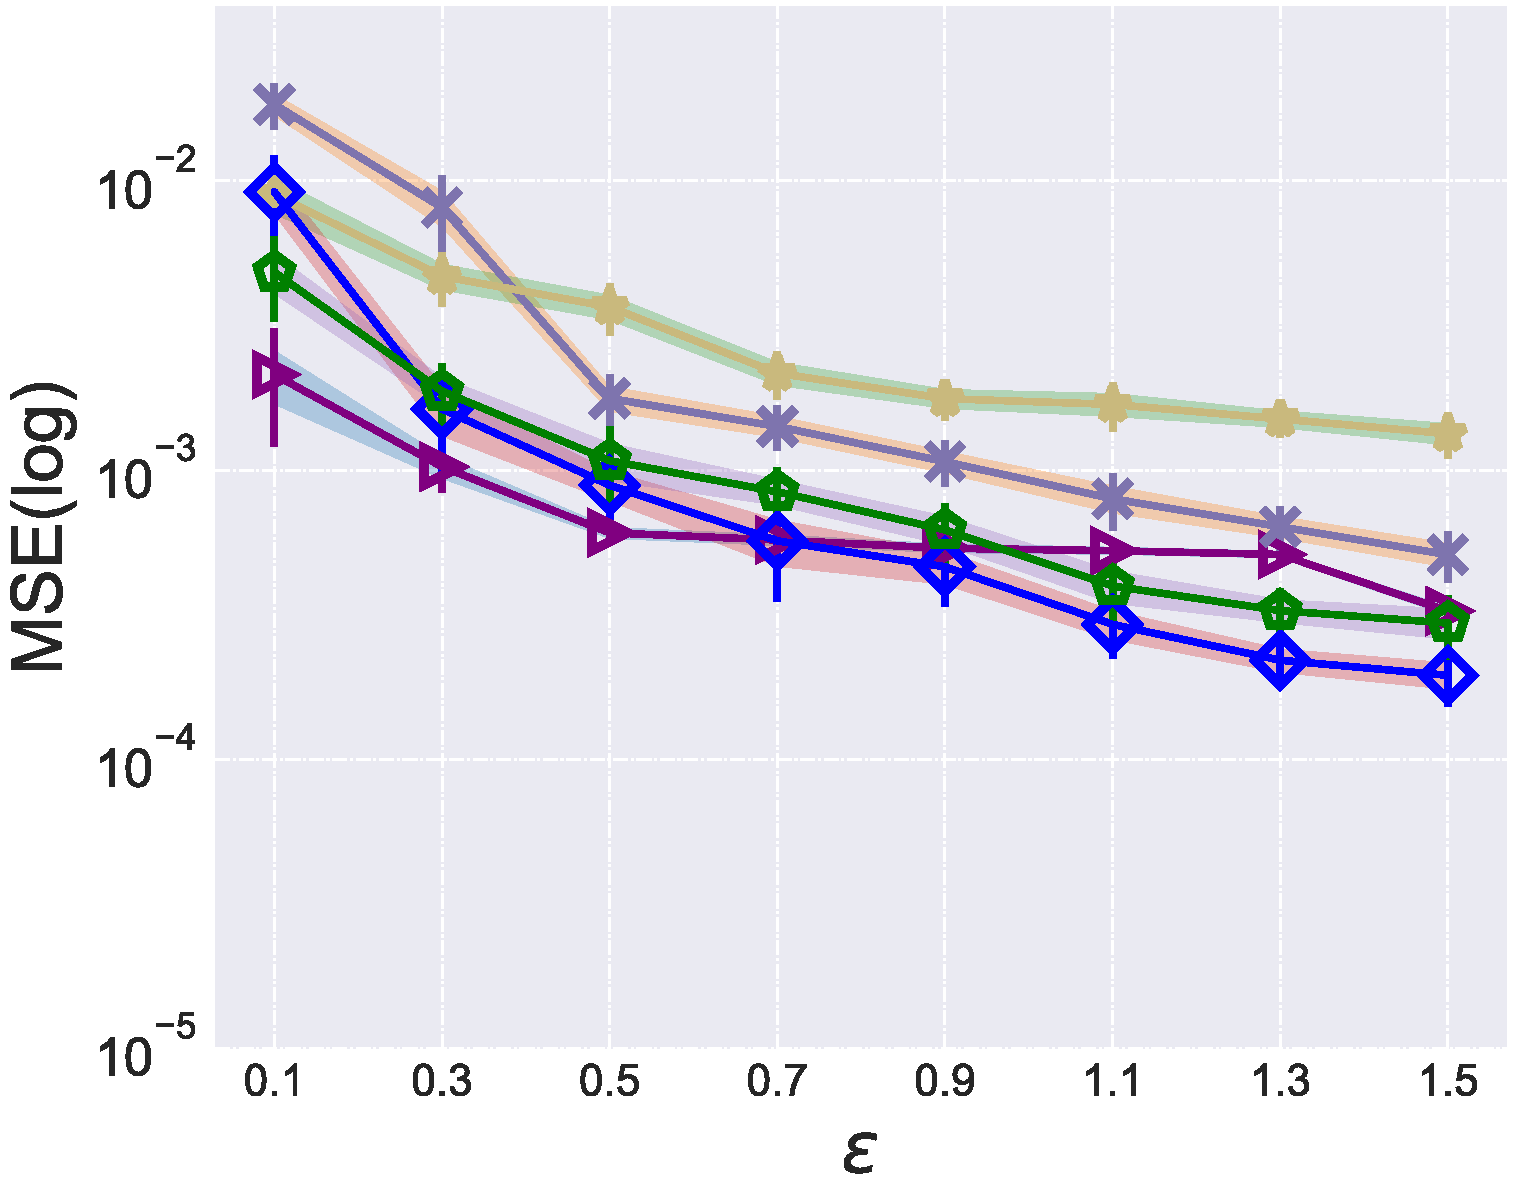
\includegraphics[width=0.24\hsize]{figure/ldp_range_query/figures_experiment_result/overall_result/0406_CI_Rand_ep-Three_Normal08-Set_10_6-Domain_6_6_6.pdf.pdf}}
    \subfigure[\Gaussian~(3), $10^7$, vary $\epsilon$]{\label{fig:Three_Normal08-Set_10_7-Domain_6_6_6}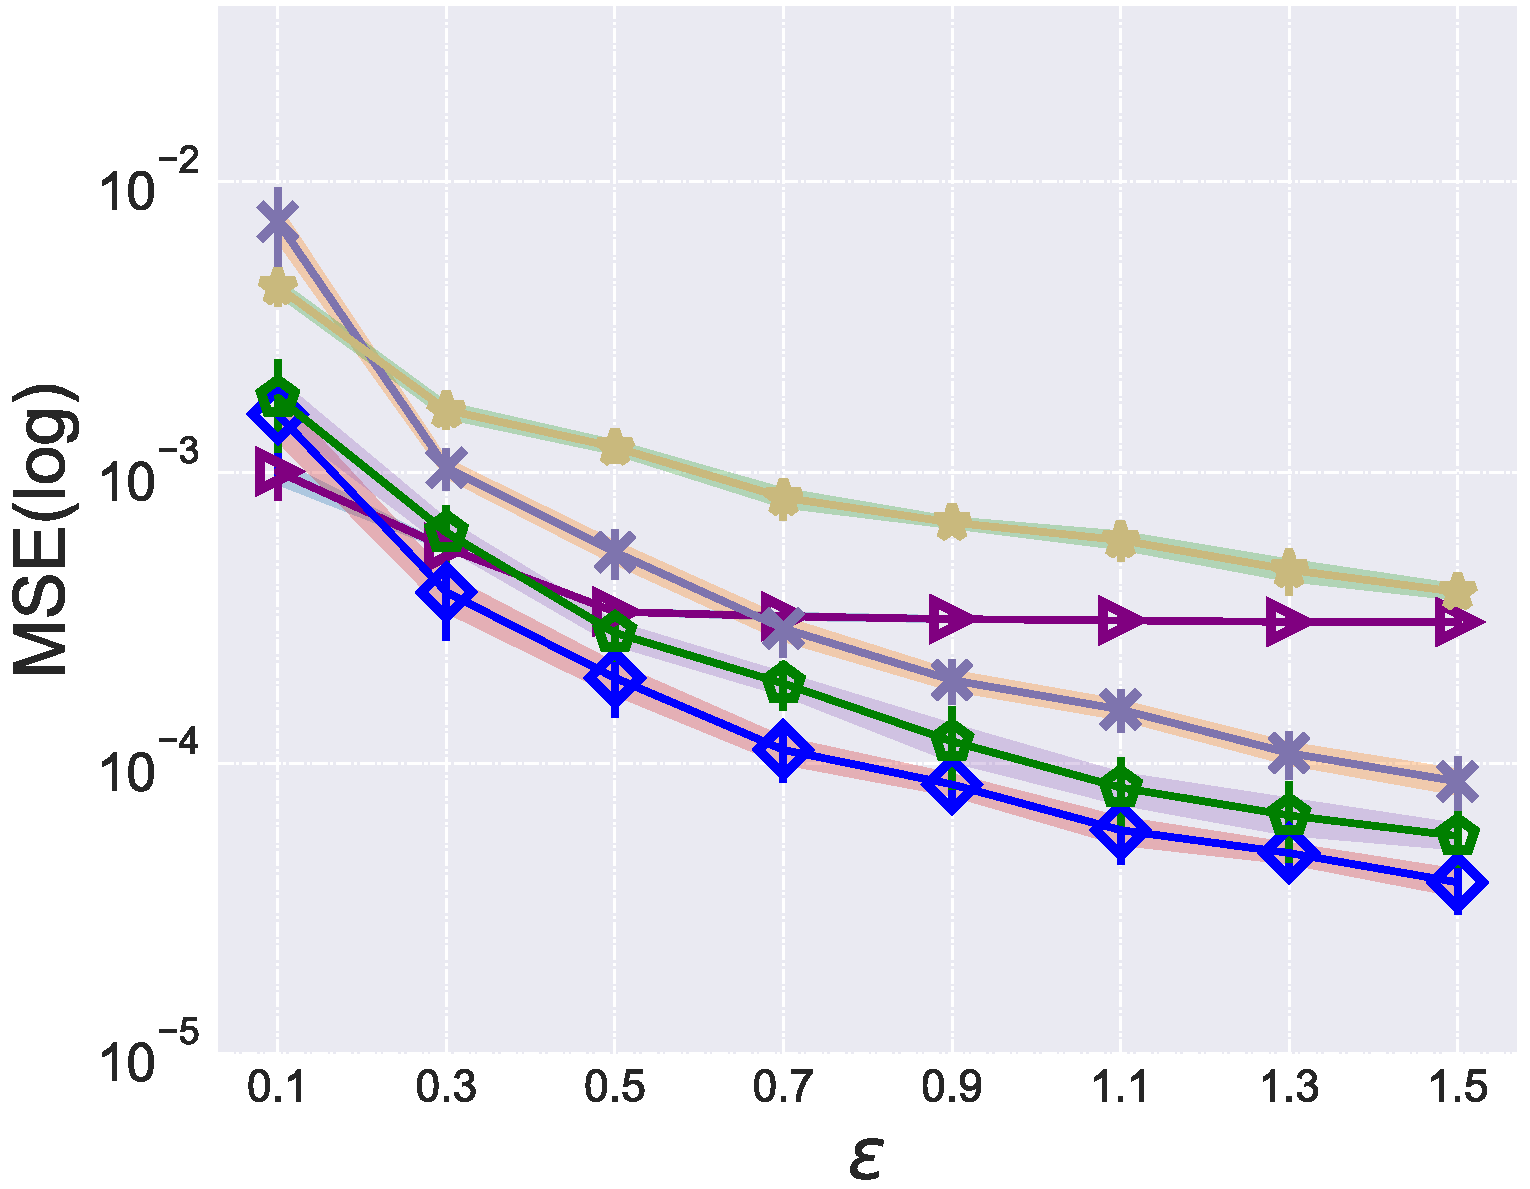
\includegraphics[width=0.24\hsize]{figure/ldp_range_query/figures_experiment_result/overall_result/0406_CI_Rand_ep-Three_Normal08-Set_10_7-Domain_6_6_6.pdf.pdf}}
    \subfigure[\Laplacian~(5), $10^6$, vary $\epsilon$]{\label{fig:Five_Laplace08-Set_10_6-Domain_6_6_6_6_6}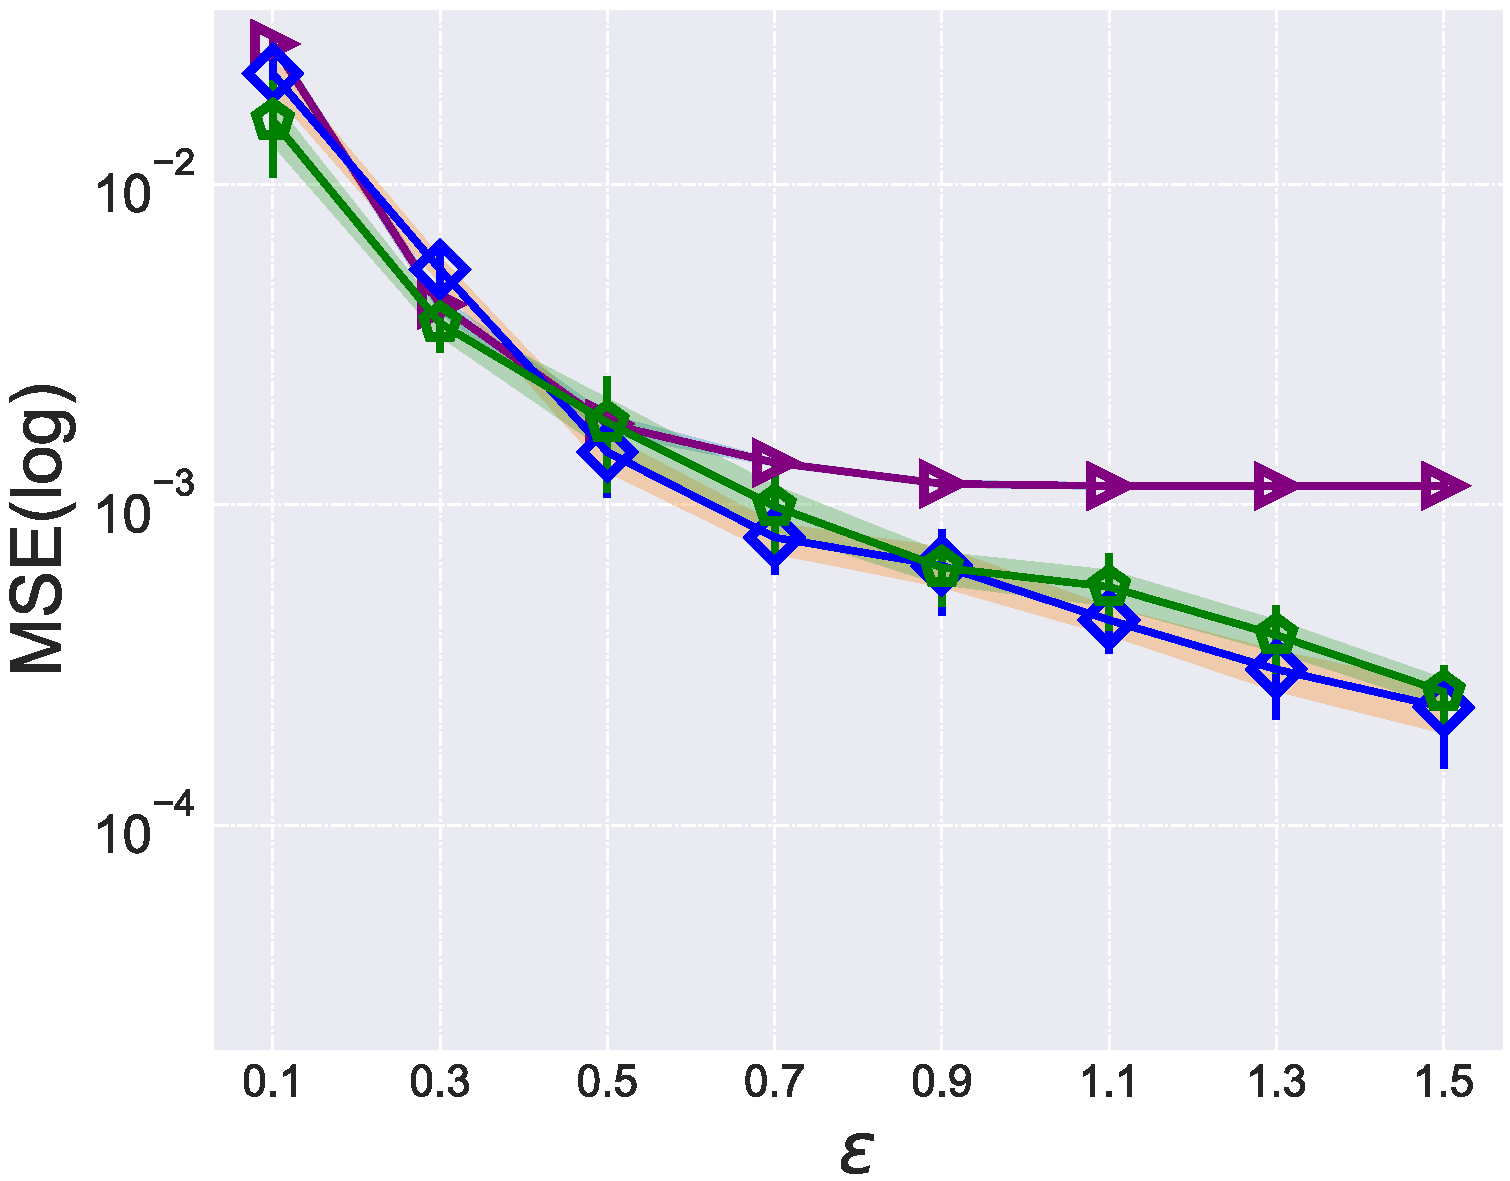
\includegraphics[width=0.24\hsize]{figure/ldp_range_query/figures_experiment_result/overall_result/0406_CI_Rand_ep-Five_Laplace08-Set_10_6-Domain_6_6_6_6_6.pdf.pdf}}
    \subfigure[\Laplacian~(5),$10^7$, vary $\epsilon$]{\label{fig:Five_Laplace08-Set_10_7-Domain_6_6_6_6_6}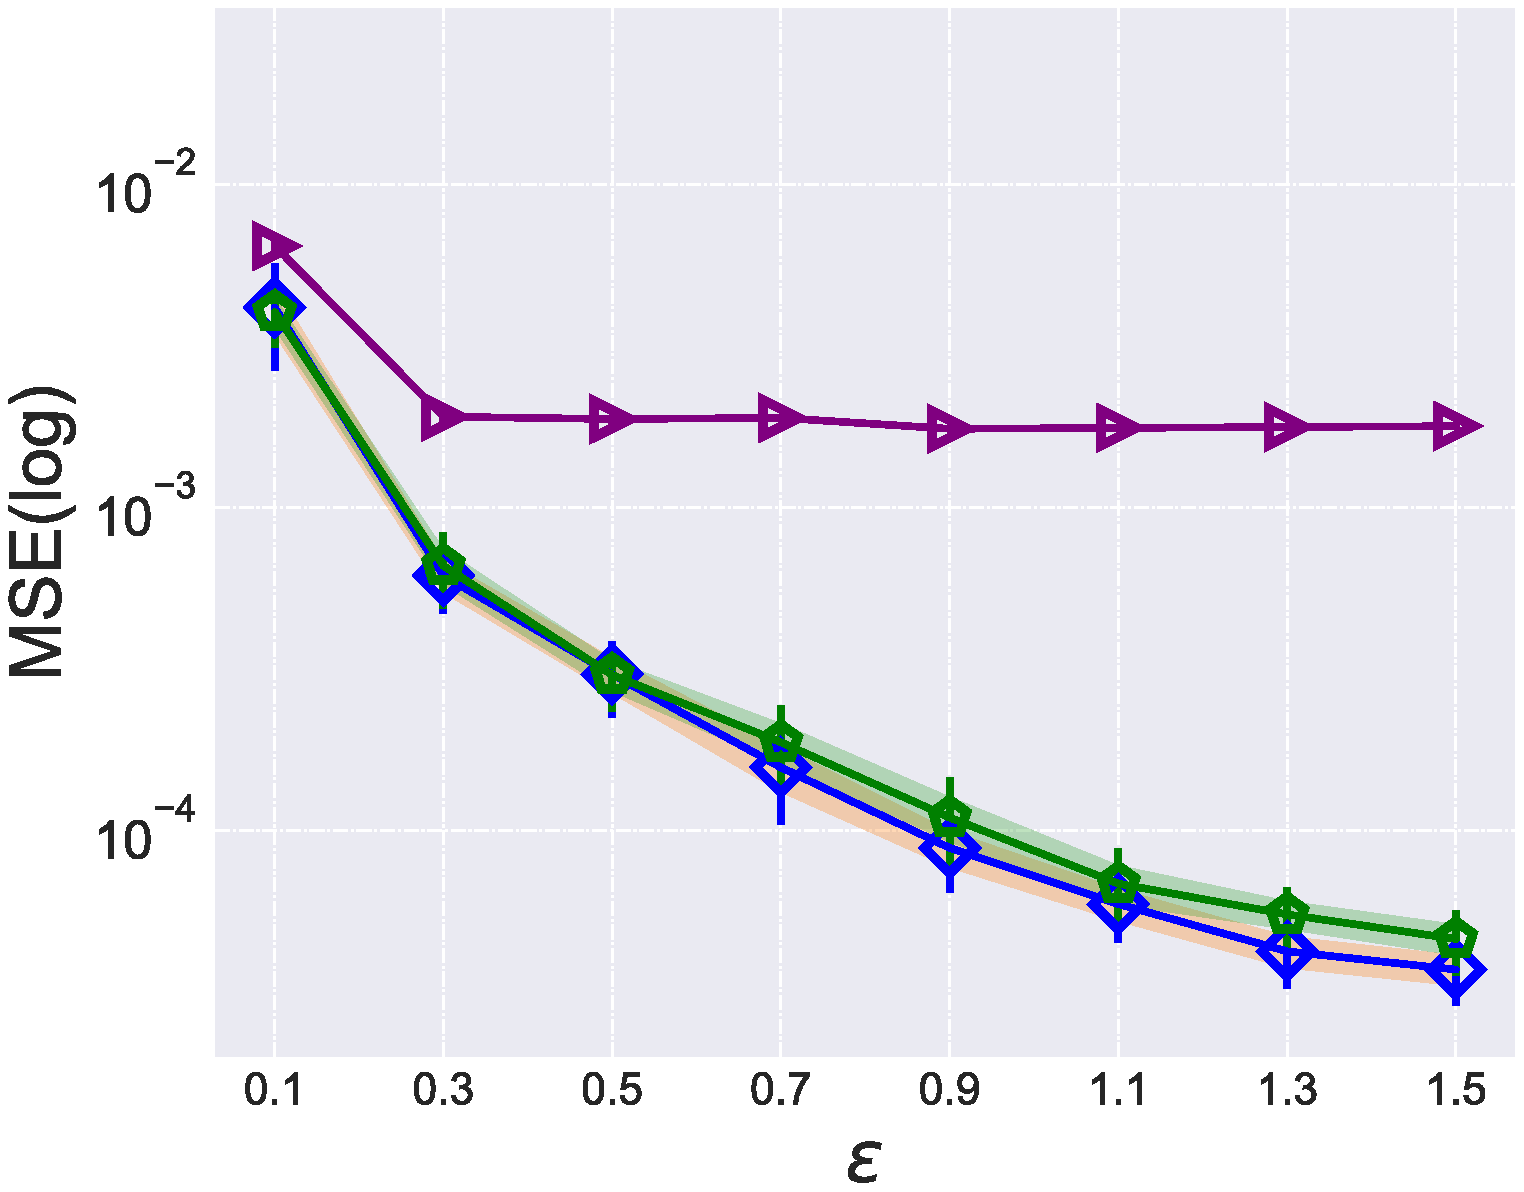
\includegraphics[width=0.24\hsize]{figure/ldp_range_query/figures_experiment_result/overall_result/0406_CI_Rand_ep-Five_Laplace08-Set_10_7-Domain_6_6_6_6_6.pdf.pdf}}
    \subfigure[\Gaussian~(5), $10^6$, vary $\epsilon$]{\label{fig:Five_Normal08-Set_10_6-Domain_6_6_6_6_6}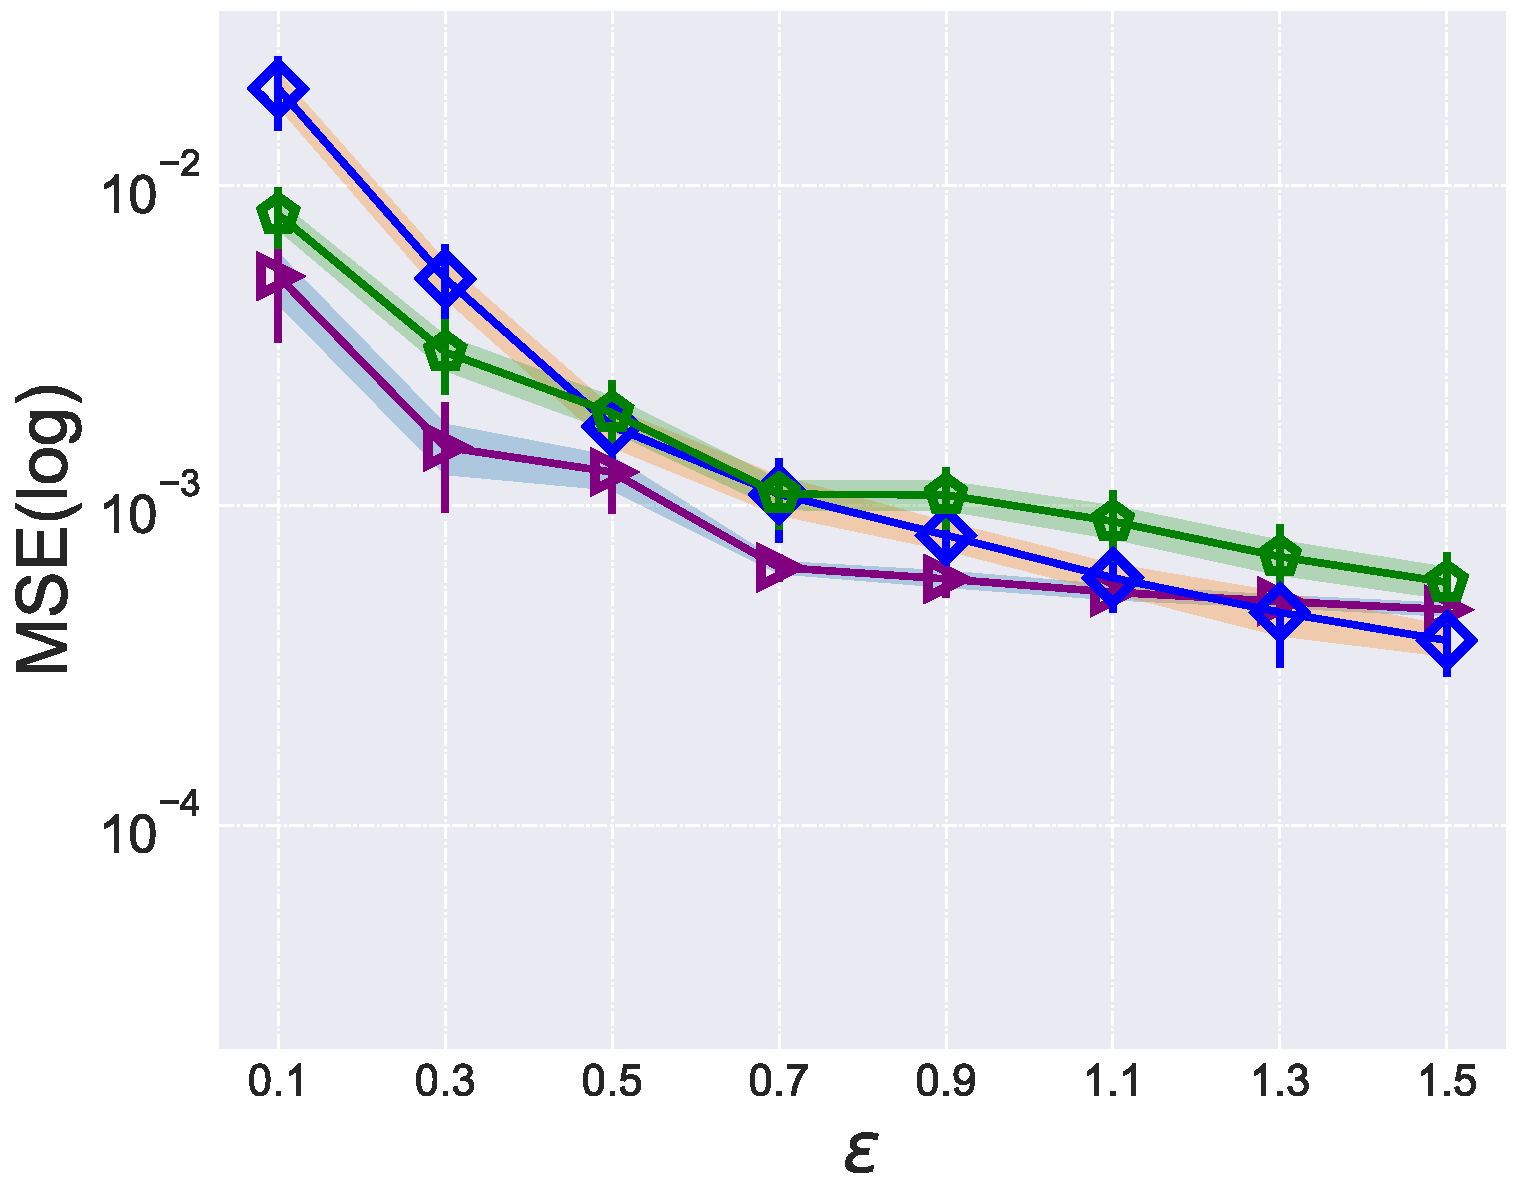
\includegraphics[width=0.24\hsize]{figure/ldp_range_query/figures_experiment_result/overall_result/0406_CI_Rand_ep-Five_Normal08-Set_10_6-Domain_6_6_6_6_6.pdf.pdf}}
    \subfigure[\Gaussian~(5), $10^7$, vary $\epsilon$]{\label{fig:Five_Normal08-Set_10_7-Domain_6_6_6_6_6}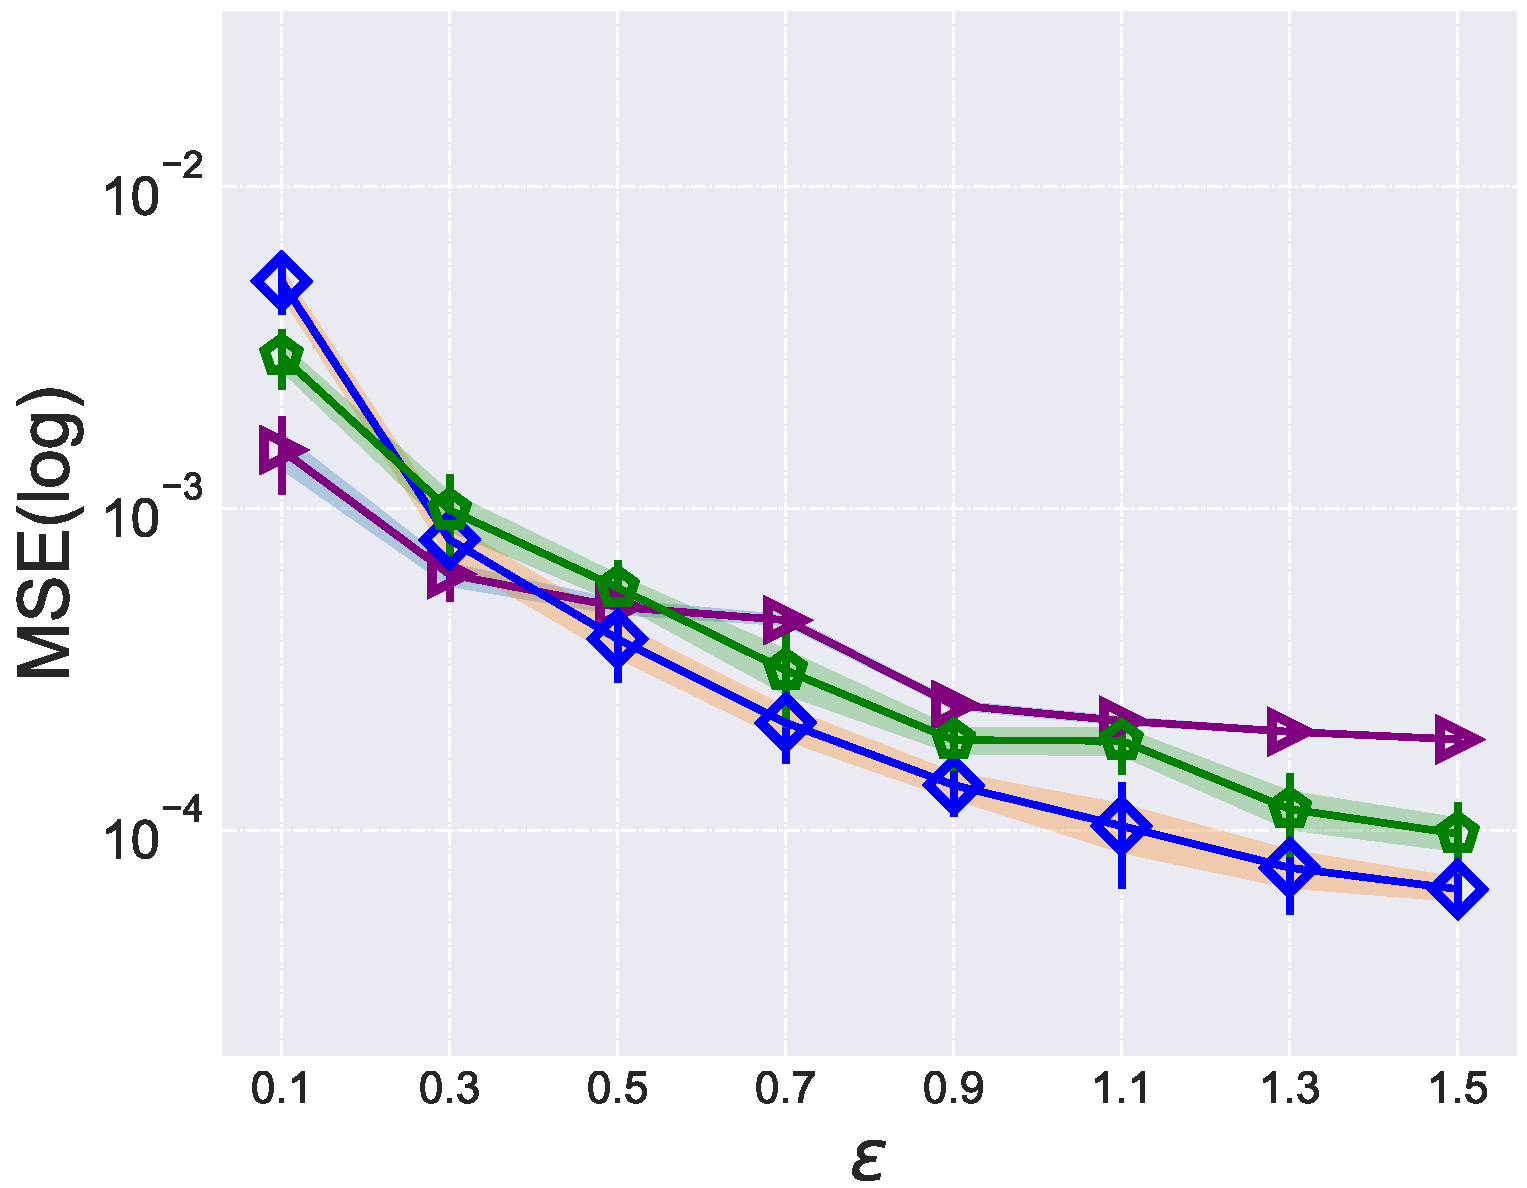
\includegraphics[width=0.24\hsize]{figure/ldp_range_query/figures_experiment_result/overall_result/0406_CI_Rand_ep-Five_Normal08-Set_10_7-Domain_6_6_6_6_6.pdf.pdf}}
    \subfigure{
\includegraphics[width=0.85\textwidth]{figure/ldp_range_query/figures_others/comparison_3D_legend5.pdf.pdf}}  
    \vspace{-0.1cm}
    \caption{Comparison of different methods on high-dimensional \Laplacian and \Gaussian datasets under various privacy budgets. \de and \lle respectively represent two high-dimensional expansion methods, \ie, ``direct estimation'' and ``leveraging low-dimensional estimation''. \myHDG is a baseline method. The results are shown in log scale.}
    % \vspace{-0.6cm}
    \label{3,5-dim overall compare}
\end{figure*}

\begin{figure*}[!h]
    \centering
    \subfigure[\Laplacian, $10^6$, $64^m$]{
    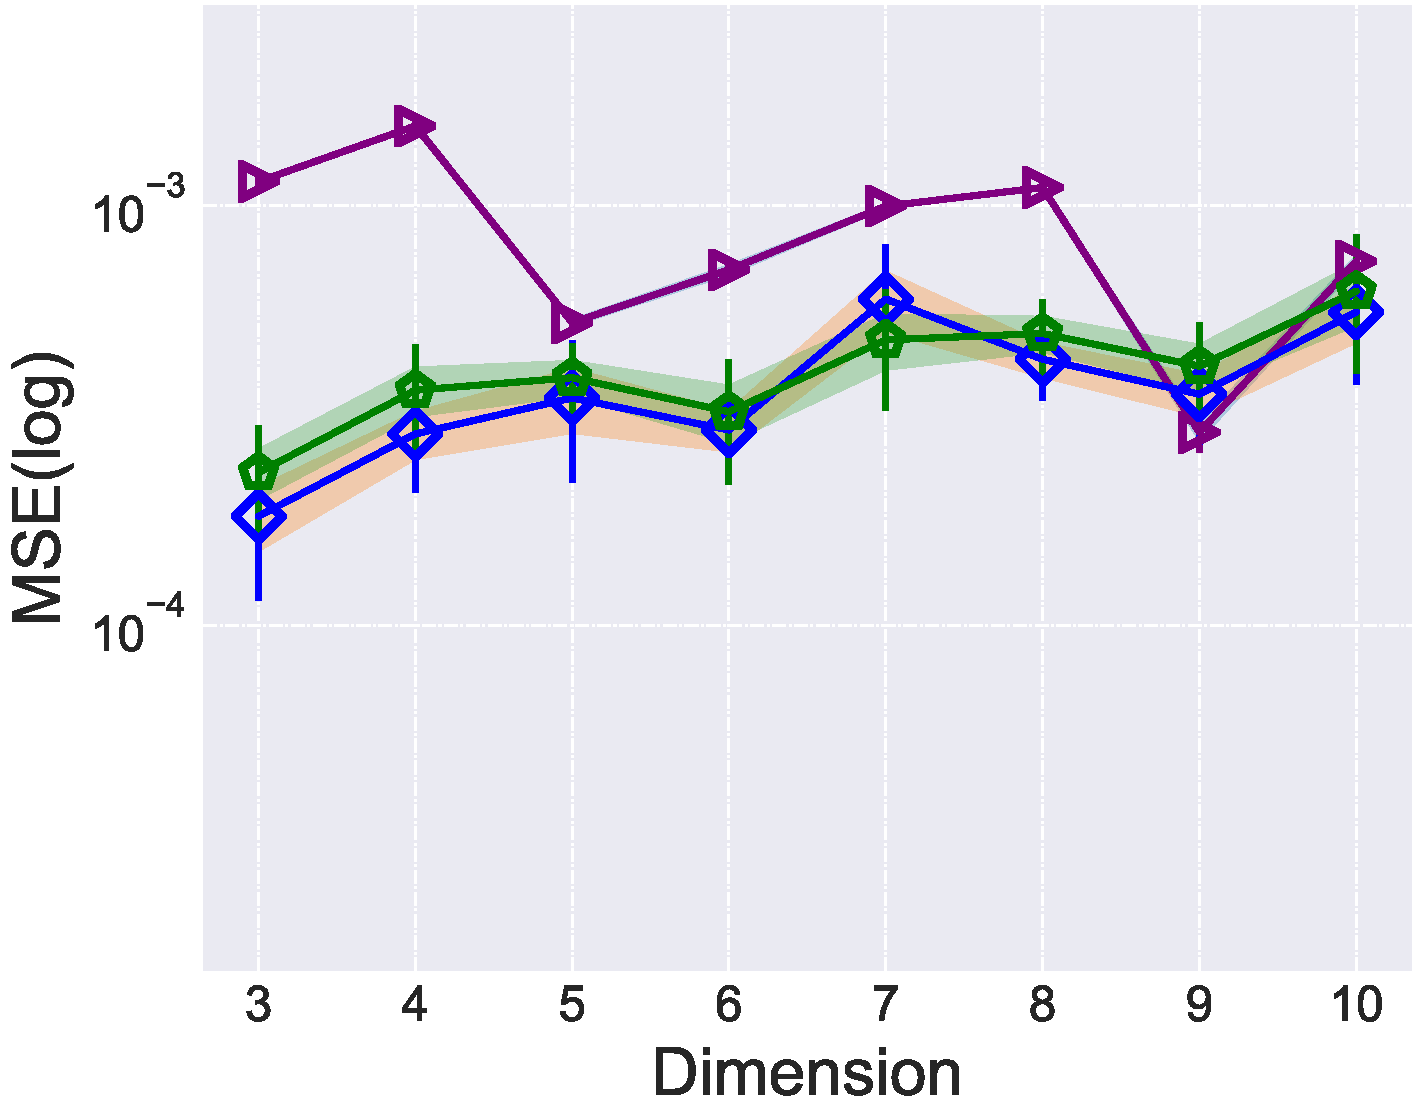
\includegraphics[width=0.23\hsize]{figure/ldp_range_query/figures_experiment_result/various_dimension/0416_CI_Rand-Attribute-Ten_Laplace08-Set_10_6.pdf.pdf}
    \label{fig: Attribute-Ten_Laplace08-Set_10_6}
    }
    \subfigure[\Laplacian, $10^7$, $64^m$]{
    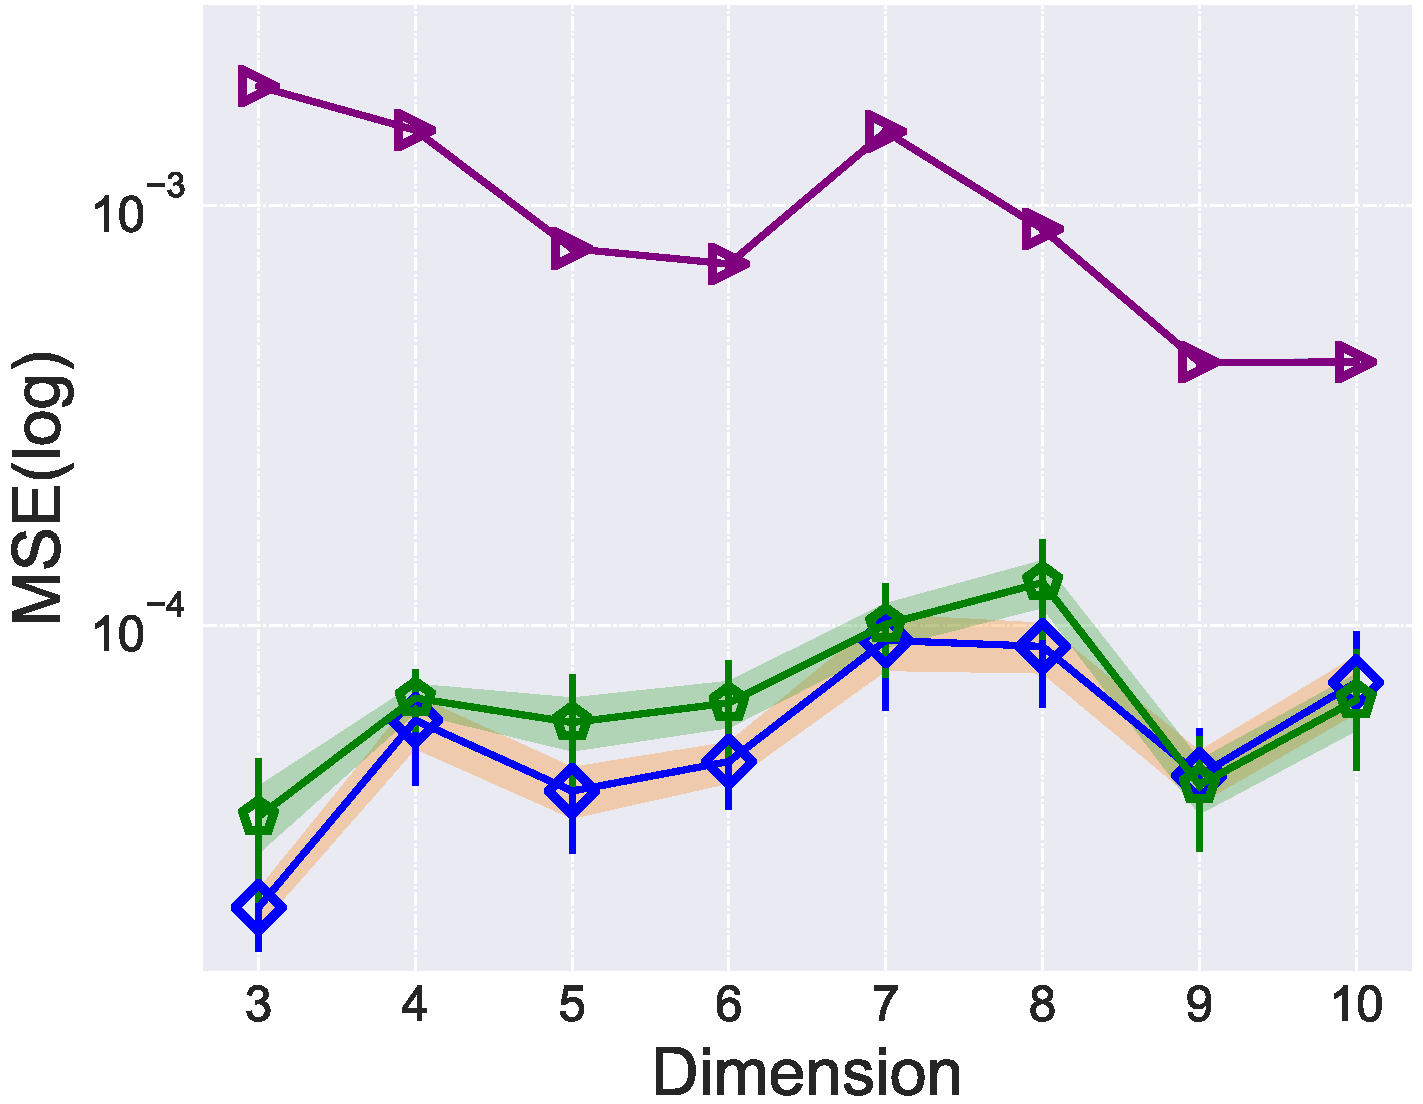
\includegraphics[width=0.23\hsize]{figure/ldp_range_query/figures_experiment_result/various_dimension/0416_CI_Rand-Attribute-Ten_Laplace08-Set_10_7.pdf.pdf}
    \label{fig: Attribute-Ten_Laplace08-Set_10_7}
    }
    \subfigure[\Gaussian, $10^6$, $64^m$]{
    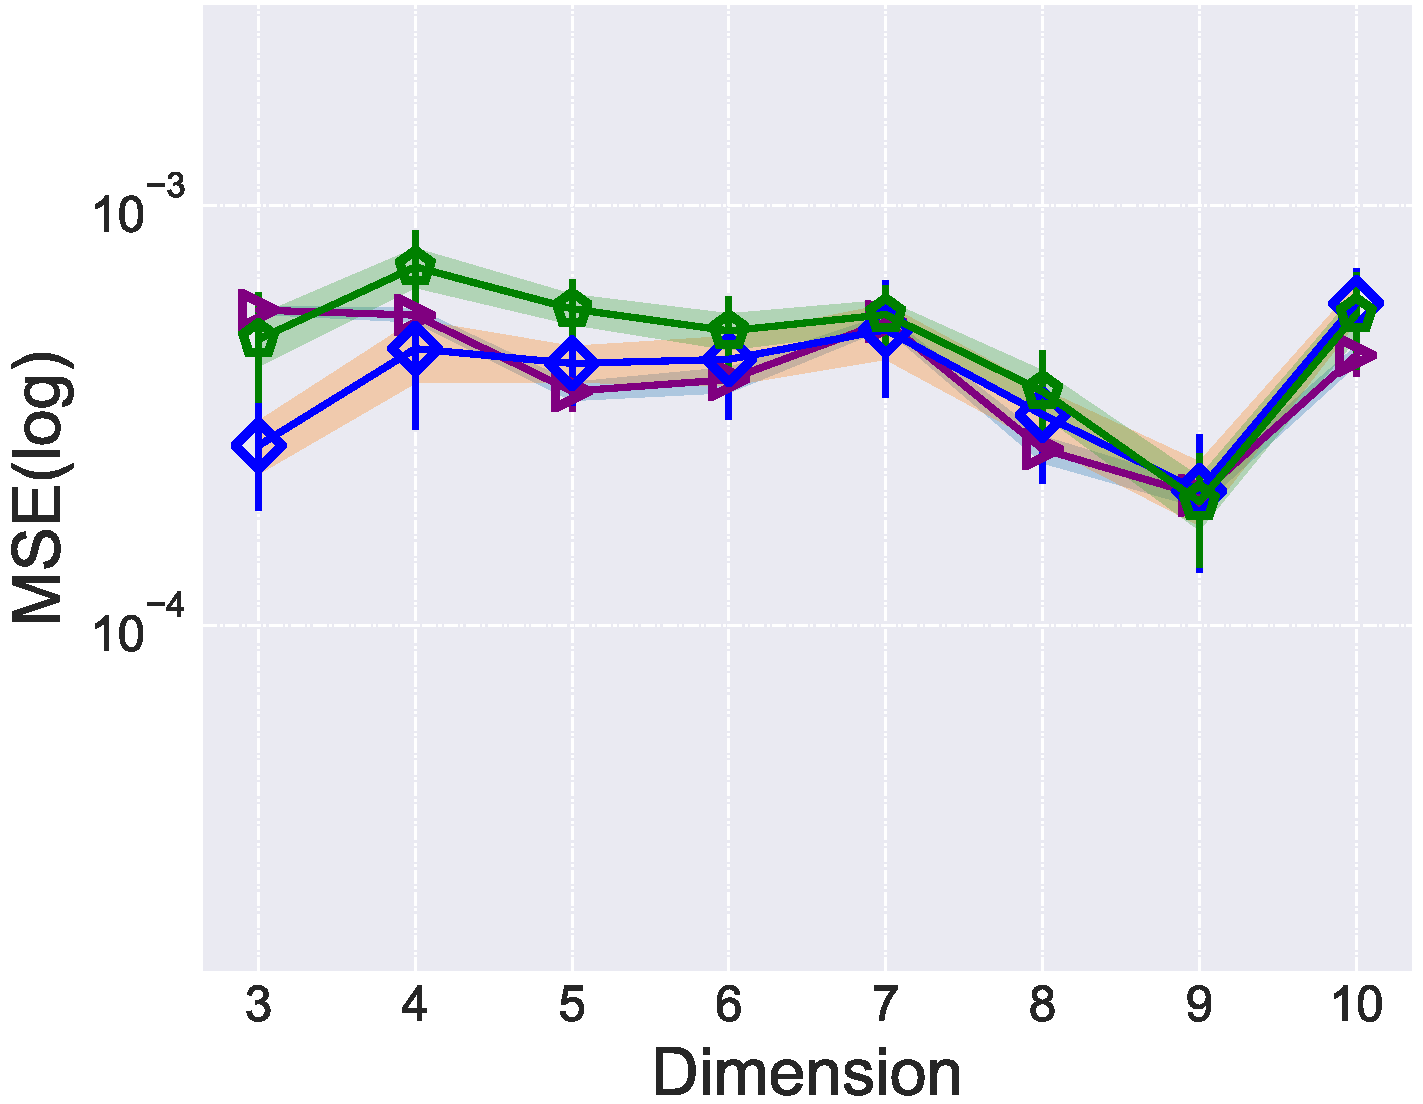
\includegraphics[width=0.23\hsize]{figure/ldp_range_query/figures_experiment_result/various_dimension/0416_CI_Rand-Attribute-Ten_Normal08-Set_10_6.pdf.pdf}
    \label{fig: Attribute-Ten_Normal08-Set_10_6}
    }
    \subfigure[\Gaussian, $10^7$, $64^m$]{
    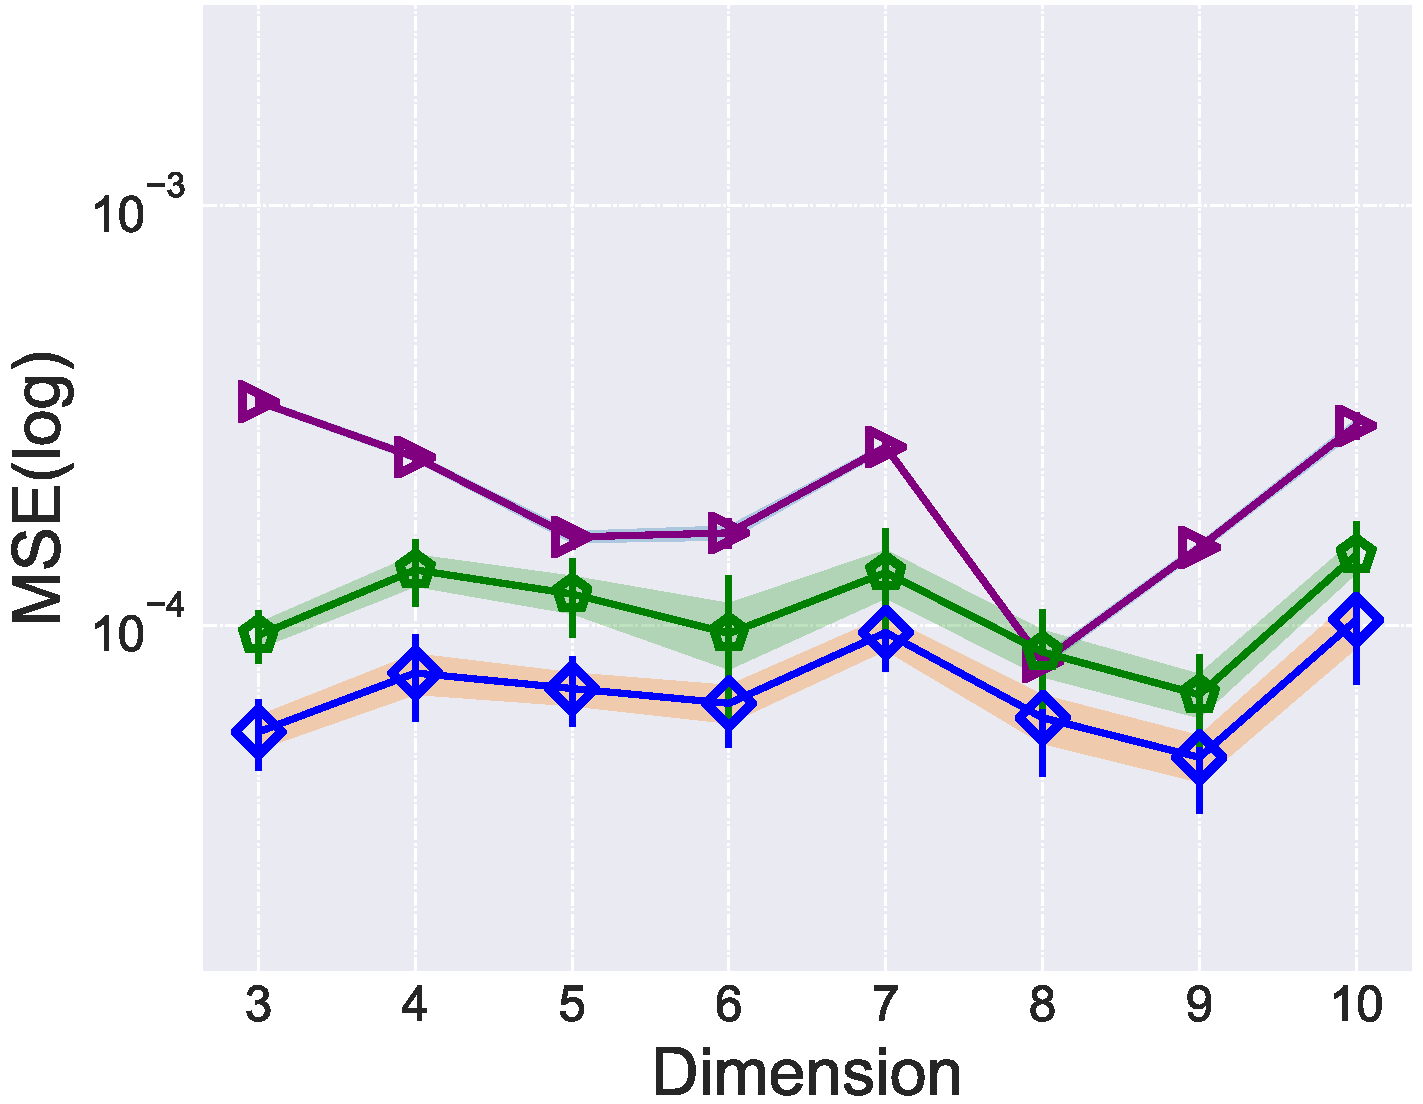
\includegraphics[width=0.23\hsize]{figure/ldp_range_query/figures_experiment_result/various_dimension/0416_CI_Rand-Attribute-Ten_Normal08-Set_10_7.pdf.pdf}
    \label{fig: Attribute-Ten_Normal08-Set_10_7}
    }
    \subfigure{
\includegraphics[width=0.55\textwidth]{figure/ldp_range_query/figures_others/comparison_3D_legend3.pdf.pdf}}  
    \vspace{-0.1cm}
    \caption{The MSE of different methods when varying data dimension $m$ with $\epsilon = 1.1$. The results are shown in log scale. }
    % \vspace{-0.4cm}
    \label{fig: varying attribute dimension}
\end{figure*}

在本小节中,我们评估 \myahead 在高维场景下的表现。
基于\autoref{2-dim overall compare}和\autoref{2-dim correlation}的实验结果,\myHDG 和 \myahead 的查询精度对数据域大小不敏感。
因此,我们将数据域大小设置为 $|D|=2^6$ ,
并分别从高维 \Laplacian 和 \Gaussian 分布中采样 $10^6$ 和 $10^7$ 条记录的合成数据集进行实验。

\mypara{不同高维场景扩展方法下的算法查询精度}
回顾 \autoref{Extension to Multi-dimensional Settings} 中的两种扩展方法,即 \de 和 \lle。
我们比较了这两种高维扩展方法在三维范围查询下的 MSE。
对于高于三维的查询,因为\de 方法计算时间过长,我们在实验中只考虑\lle。
从 \autoref{3,5-dim overall compare} 中可以观察到,
\lle 下的 \myahead 比 \de 的 MSE 要低。
通过 \de 得到的子域是等边的高维立方体,
\myahead 倾向于使用底层的节点,导致在查询结果中积累了较多的误差。
例如,对于一个三维查询 $[1,1]\times[1,8]\times[1,8]$,其中数据集的范围为 $[1,8]\times[1,8]\times[1,8]$,\myahead 选择使用底层的 64 个叶节点来回答查询,
而不是使用具有更大子域的高层节点,这会导致误差的累积。
尽管 \lle 需要将用户分组,并从每个用户组上传数据中计算不同属性组合的频率分布。
相对于 \de, \lle 在估计每一层的频率分布时持有较少的用户上传数据,
但是 \lle 的最大熵优化步骤融合了更多的二维分布信息,得到了更小的 MSE。

\mypara{不同隐私预算下的算法查询精度}
\autoref{3,5-dim overall compare} 展示了算法在三维和五维数据集上的查询结果。
我们采用相关系数 $r=0.8$ 来量化属性之间的相关性,保持了与文献{\rm\parencite{yang2020answering}}相同的设置。

根据实验结果,我们总结出以下结论。
% 这些结果与我们在 \autoref{Extension to Multi-dimensional Settings} 中的分析一致。
1)\myahead 对数据分布的变化具有鲁棒性。
回顾\autoref{Selection parameters}中参数$\theta$和$B$的推导过程,\myahead 的参数设置对用户数据的分布没有特定要求。
当整个数据域被自适应地划分时,相同的$\theta$可以确保区间的频率具有类似的总体误差。
因此,从\autoref{fig:Three_Laplace08-Set_10_7-Domain_6_6_6},\autoref{fig:Three_Normal08-Set_10_7-Domain_6_6_6}(或\autoref{fig:Five_Laplace08-Set_10_7-Domain_6_6_6_6_6},\autoref{fig:Five_Normal08-Set_10_7-Domain_6_6_6_6_6})来看,
\myahead 在不同的数据集上表现类似。
在相同的数据集参数下,\myHDG 使用相同粒度的一、二维网格来聚合用户数据,然后基于网格内用户满足均匀分布的假设回答查询。
因此,\myHDG 在频率分布更不均匀的\Laplacian 数据集上的均方误差大于其在\Gaussian 数据集上的均方误差。
2)对于高维查询,\myahead 的性能更依赖较大的用户数据规模。
回顾\autoref{Extension to Multi-dimensional Settings},\myHDG 只需要将总体用户分成与两两属性组合数量相同的用户组,而\myahead 还需要用户组进一步划分到二维树的不同层。
对于一个三维数据集,属性数据域大小为$|D|=64$,\myahead 将用户随机划分为$C_3^2 \cdot 6$组,而\myHDG 只需将用户分为$C_3^2 + C_3^1$组。
这种情况下,\myahead 中每个组的用户记录数是\myHDG 组的一半,导致\myahead 算法中的噪声误差翻倍。
因此,从\autoref{fig:Three_Laplace08-Set_10_6-Domain_6_6_6}和\autoref{fig:Three_Laplace08-Set_10_7-Domain_6_6_6}中可以看出,
\myahead 相比于\myHDG 的查询精度优势随着用户记录减少而减小。

\mypara{不同数据维度下的算法查询精度}
我们评估了\myahead 和 \myHDG 在高维\Laplacian 和\Gaussian 数据集上的查询精度。其中,数据维度从三维变化到十维,属性相关系数为 $r=0.8$。
从\autoref{fig: varying attribute dimension} 可以看出,\myahead 对数据维度的变化具有鲁棒性。
回顾\autoref{Extension to Multi-dimensional Settings},随着数据维度$m$的增加,属性组合数量增大。
\lle 需要将用户划分为更多的用户组,即降低了用于估计每个二维\myahead 树频率分布的用户数据数量。
例如,当$m=3$时,属性组合数为$C_3^2=3$,当$m=10$时,属性组合数为$C_{10}^2=45$。
另一方面,由于\lle 使用与高维查询相关的$2^m$个二维查询结果构建高维查询结果(回顾\autoref{Extension to Multi-dimensional Settings}),
因此,\lle 的最大熵优化步骤包含更多维度的查询结果信息。
综上,\lle 方法随着维度的增加,查询结果的MSE几乎保持不变。

\section{本章小结}
本文提出了一种新的本地差分隐私协议,其核心贡献是基于自适应层级分解解决了一维和多维范围查询问题。
我们的方法在满足严格的本地差分隐私保证的同时,实现了优越的查询精度。
通过理论分析和大量实验评估,我们展示了\myahead 可以很好的权衡范围查询的查询精度和用户数据的隐私保护强度,相对于现有方法具有显著的优势。
此外,通过不同的实验参数设置,我们总结出多个有助于在实际中部署\myahead 的结论。




% \begin{figure}[htbp]
%     \centering
%     \includegraphics[width=.3\linewidth]{example-image-a}
%     \caption{\label{fig:fig-placeholder}图片占位符}
% \end{figure}

\chapter{第三章~~强化学习模型关键参数泄露风险评估}

本章摘要: 
深度强化学习(DRL)已被应用于许多关键系统,例如智能电网、交通控制、自动驾驶等。
为了保护知识产权和减少潜在的安全风险,实际中部署的DRL模型通常只具有黑盒访问权限,即输入环境状态并给出相应的执行动作。
例如,模型神经网络的结构和优化过程中的参数通常不会向用户公开,以免侵犯模型拥有者的知识产权或增加系统的脆弱性。
所以,探究模型的输入状态和输出动作是否具有泄露了超参数设置的风险非常重要。
为了有效地评估模型参数泄露风险,我们面临两个主要挑战:
1)从具有黑盒访问权限的模型中获得的信息有限;
2)不同超参数对DRL模型的行为影响具有强耦合性。

我们提出了一种针对DRL模型的超参数窃取攻击(\sysname),可以用来评估基于不同框架的模型的参数泄露风险。
我们观察到DRL模型在不同的超参数设置下在相同任务上具有不同的行为偏好。
基于该事实,我们设计了两种状态生成机制来刺激DRL模型的产生行为分歧,
并训练了一个攻击模型来刻画DRL模型的行为和超参数设置之间的关系。
通过使用多个DRL模型和环境,我们全面地展示了\sysname 的超参数窃取效果,
例如,在PPO模型和CartPole环境上,所提方法推断准确度超过$90\%$。
另外,\sysname 可以作为增强其他下游攻击的基础,例如\sysname 可以有效提高对抗样本攻击的在不同模型之间的可迁移性。

关键词:模型关键参数;数据泄露;强化学习

\section{引言}

深度强化学习(Deep Reinforcement Learning, DRL)结合了深度神经网络(Deep Neuron Network, DNN)强大的拟合能力,
成为一种具有广阔应用前景的机器学习范式。
例如AlphaGo Zero~\cite{SSSAHGHBLB17},
在三天内通过自我对弈而无需人类数据,获得了击败人类冠军的能力。
DRL还成功地应用于许多复杂的决策任务,如自动驾驶~\cite{FHOL18}、机器人控制~\cite{A17}、金融交易~\cite{DBKRD17}、电子竞技~\cite{SSSAHGHBLB17,BBCCDDFFHHJGOPPPRSSSSSTWZ19}等。

DRL模型通常只开放输入、输出接口以提供服务,即黑盒访问权限,
一方面,因为泄露模型参数设置的细节可能会使模型更容易受到数据层面的恶意攻击,
如对抗样本攻击~\cite{HPGDA17, BM17, LHLSLS17, KS17}和模型后门攻击~\cite{KWSL20,YIRV19,KWJL20,WSLMJ21,WJWGXS21}。
另一方面,DRL的模型参数设置属于知识产权,泄露将会造成模型所有者的财产损失。
综上,研究在黑盒访问权限下进行DRL模型参数设置泄露风险的评估是至关重要的。

现有文献已经探究了针对有监督深度学习模型的参数设置窃取攻击~\cite{OASF18,WG18}。
但是,这些技术不能直接应用于DRL模型。
在有监督学习场景中,攻击者可以使用训练数据集作为高质量的输入进行模型参数嗅探。
因为DRL模型通常是从与环境的交互中学习,DRL攻击者没有现成的嗅探数据。


在本章中,我们对DRL模型的超参数泄露风险进行评估。
评估的关键依据是DRL模型在某些状态下不一致的行为(行为分歧)将暴露它们的超参数配置信息。
基于这个观察,我们的方法首先构建一系列状态,收集DRL模型的行为分歧,然后利用分类器根据状态和预测的行动来揭示受害者黑盒DRL模型的架构和优化过程。由于行为分歧包含更多的超参数设置知识,所以在具有高质量状态序列的情况下,窃取攻击将变得更加有效,即刺激更多的行为分歧。

我们提出了两种状态生成机制来构建状态序列。 
被动状态生成方法基于被动记录DRL模型与环境之间的交互来构建状态序列,解决了上面提到的第一个挑战。
然而,仅直接从环境中获取状态只能弱化DRL模型生成分歧行动的刺激。
为了使具有相同超参数设置的智能体表现出相似的行为,而具有不同超参数设置的智能体表现出不同的行为,我们进一步提出了一种主动状态生成方法。
具体来说,除了训练分类器预测超参数设置外,主动方法还反向传播分类器模型的部分损失并优化状态。
优化后的状态可以引导具有不同超参数设置的DRL模型生成更多的分歧行动。
此外,我们经验证明,不断调整的状态可以减缓分类器的过拟合,并进一步提高准确性。

我们的实验结果表明,在多个DRL模型和环境下,超参数激活函数的窃取准确率超过$60\%$,甚至在PPO智能体上超过$90\%$。
我们进一步评估了影响窃取攻击性能的四个代表性影响因素,即受害DRL模型的奖励标准,超参数耦合,状态-动作序列的长度以及影子DRL模型的数量。
总之,我们对\sysname 的实际采用获得了三个重要观察结果。
首先,具有更高奖励标准的DRL模型存在更高的超参数泄漏风险,这警示DRL从业者,因为随着DRL性能的提高,超参数隐私变得更加容易受到攻击。
其次,超参数对模型动作偏好有不同的影响强度。
例如,攻击者可以轻松地从DRL模型的行为中区分激活函数或优化器,而很难区分学习率。
第三,主动窃取攻击方法以更少的状态生成和DRL模型训练成本获得了表现优异的结果,这使\sysname 成为一种高效的超参数窃取机制。
此外,我们评估了一种潜在的防御方法,即仅发布预测动作而非置信度值(后验概率),以减少对攻击者可访问的信息。
然而,在某些设置中,主动窃取攻击方法的窃取准确率仍比基线高$20\%$。
最后,我们以对抗攻击为案例研究,并展示了针对黑盒DRL模型的对抗性示例在有或无超参数信息的情况下的可转移性改进,以证明我们的窃取攻击的必要性。

综上,我们的贡献可分为三个方面:
\begin{itemize}
\item 我们提出了首个针对DRL模型的超参数窃取框架\sysname,揭示了当前DRL模型参数泄露风险。
\item 我们在六种不同的DRL模型和环境组合上展示了\sysname 的有效性。我们系统地分析了各种实验因素,并总结出了一些重要的关于实践中采用\sysname 的观察结果。
\item 通过显著提高对抗状态的可迁移性,我们展示了提出的\sysname 可以作为进一步攻击的基础,这提醒人们注意超参数窃取攻击的隐私风险。
\end{itemize}

\section{预备知识}
\subsection{强化学习问题}
\label{sec:Reinforcement Learning Problem}
在强化学习问题中,模型的目标是寻找一种最优或接近最优的策略,以最大化完成一段序列决策后累积的“奖励函数”或其他用户提供的奖励信号。
模型的学习过程与动物心理学中的条件反射实验相似。
例如,假设在投喂食物(奖励)之前播放音乐,
那么狗倾向于将声音与食物联系起来,并在仅听到声音刺激时流口水~\cite{PG41}。

强化学习问题可以被建模为一个马尔科夫决策过程(Markov Decision Process,MDP)问题,通常由四个变量组成:
\begin{itemize}
% \setlength\itemsep{-0.3em}
\item 状态空间 $\mathbb{S}$ 包含模型的所有可能状态,其中 $s_t \in \mathbb{S}$ 表示时间步 $t$ 时的模型状态。
\item 动作空间 $\mathbb{A}$ 包含模型的所有可能动作,其中 $a_t \in \mathbb{A}$ 表示时间步 $t$ 时的模型动作。
\item 状态转移函数 $\mathcal{T}$ 定义为从状态-动作对到新状态的概率映射 $\mathcal{T}: (\mathbb{S} \times \mathbb{A}) \times \mathbb{S} \rightarrow [0, 1]$。
\item 奖励函数 $\mathcal{R}: \mathbb{S} \times \mathbb{A} \rightarrow \mathbb{R}$ 输出在状态 $s_t$ 上采取动作 $a_t$ 时预期的奖励 $r_t \in \mathbb{R}$。
\end{itemize}
训练后的模型学习到一个策略 $\pi$,
它将状态-动作对映射到概率分布 $\pi: \mathbb{S} \times \mathbb{A} \rightarrow [0, 1]$,以最大化累计奖励。
\begin{equation}
    \pi^{*}=\underset{\pi}{\arg \max } \sum_{t=t_{0}}^{T} \sum_{a_{t} \in \mathbb{A}} \gamma^{t-t_{0}} \mathcal{R}\left(s_{t}, a_{t}\right) \pi\left(s_{t}, a_{t}\right)
\end{equation}
其中,折扣因子 $\gamma$ 被用于折算累计奖励中的未来奖励,$T$ 是一个游戏回合的终止时间步,$t_0$ 是初始时间步。

\mypara{示例}
\begin{figure}[!t]
    \center
    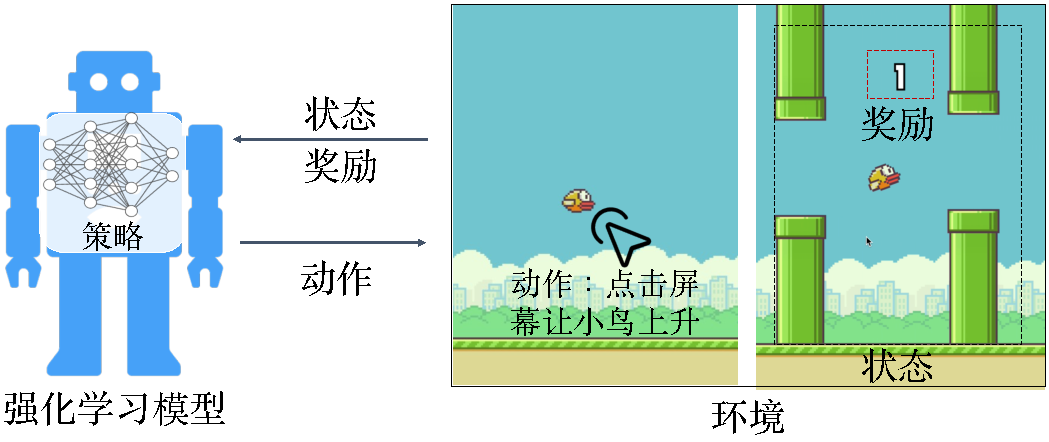
\includegraphics[width=0.6\hsize]{figure/drl_hypertheif/fig-drl-examplech.pdf}
    \caption{强化学习问题示例}
    \label{fig:running example}
\end{figure}
\autoref{fig:running example} 给出了一个运行示例,
其中模型与Flappy Bird游戏环境\footnote{\url{https://flappybird.io}} 进行互动。
状态包括鸟和障碍物的位置。
模型选择是否点击(动作)来让鸟向上飞或下落。
奖励为每次操作之后获得的分数。
模型从环境中获取状态和奖励,然后在每个时间步从动作空间中选择一个动作。
然后,环境更新状态并给予奖励。
基于环境状态、执行动作和奖励,模型训练一个策略(神经网络)来最大化累计奖励,即游戏结束时的总分数。

\subsection{强化学习模型}
\label{sec:Deep Reinforcement Learning model}
强化学习的目标是找到一种最优行为策略以获取高奖励。
基于不同的策略优化方法,我们将现有的强化学习模型分为三类。

\mypara{基于值的强化学习模型}
Q-learning是一种主要的基于值的强化学习模型 \cite{watkins1989learning},
通过最大化连续步骤中总奖励的期望值来找到最优策略。
Q-learning通过训练拟合一个用于计算状态-动作组合质量的函数:
$
\mathcal{Q}: \mathbb{S} \times \mathbb{A} \rightarrow \mathbb{R}.
$
对于基本的Q-learning算法,$\mathcal{Q}$ 在训练初始化阶段被定义为一张充满随机值的表格。
在每个时间步 $t$,模型基于当前的环境状态,选择一个执行动作 $a_t$,并收到奖励 $r_t$。
然后,环境更新状态至 $s_{t+1}$(取决于先前的状态 $s_t$ 和选择的动作 $a_t$),
模型根据交互过程中的状态、动作和奖励数据更新 $\mathcal{Q}$ 中的值。
$\mathcal{Q}$每次更新过程如下所示。
\begin{equation}
    \label{eq:q-learning-obj}
    \mathcal{Q}^{\text{new}} \leftarrow \mathcal{Q} + 
    \alpha \cdot\left(r_{t}+\gamma \max_{a} \mathcal{Q}\left(s_{t+1}, a\right)-\mathcal{Q}\left(s_{t}, a_{t}\right)\right), 
\end{equation}
其中,$\alpha \in (0,1]$ 是学习率,$\mathcal{Q}^{\text{new}}$ 的变化速度随着 $\alpha$ 的增大而加快。

如\autoref{eq:q-learning-obj}所示,Q learning使用原始的 $\mathcal{Q}$ 值和通过交互获取的新信息的加权平均值来进行更新。

然而,当状态和动作空间十分庞大时,Q-learning 很难维护和存储一个巨大的$\mathcal{Q}$。
为了解决这个问题,深度Q-learning网络(Deep Q-learning Network, DQN)~\cite{MKSGAWR13} 将深度神经网络用来拟合$\mathcal{Q}$。
凭借着神经网络在学习高维特征表示和函数逼近方面的卓越性能,DQN在围棋 \cite{SSSAHGHBLB17} 和 Atari 游戏上达到了人类专家水平~\cite{MKSGAWR13}。

\mypara{基于策略更新的强化学习模型}
相比于Q-learning通过和环境交互拟合$\mathcal{Q}$,基于策略更新的强化学习模型直接学习状态和动作之间的映射关系。
例如,REINFORCE~\cite{W92}通过梯度下降更新神经网络参数的以获得交互策略。
目前,基于策略更新的强化学习模型倾向于使用深度神经网络,如多层感知机 \cite{XLZP18} 或循环神经网络 \cite{ZMFLA16})作为策略$\pi$的载体。
基于策略更新的强化学习模型的目标函数为最大化交互累计奖励。
\begin{equation}
    \label{eq:pg-obj}
    J(\theta)=\mathbb{E}_{\left(s_{t}, a_{t}\right) \sim \pi_{\theta}}\left[\sum_{t=0}^{\infty} \gamma^{t} r_{t}\right]. 
\end{equation}
根据文献{\rm\parencite{KT99}},目标函数的梯度可写成如下方程:
\begin{equation}
    \nabla_{\theta} J(\theta)=\mathbb{E}_{\pi_{\theta}}\left[\nabla_{\theta} \log \pi_{\theta}(s, a) v_t\right], 
\end{equation}
其中 $v_t$ 是 $Q_{\pi_{\theta}}(s,a)$ 的采样值,$Q_{\pi_{\theta}}(s,a)$则表示MDP问题中真实的累计奖励函数,而 $\pi\left(s, a\right)$ 则是策略网络。

\mypara{Actor-Critic强化学习模型}
Actor-Critic 强化学习模型 \cite{MBMGLHSK16} 由两个主要的部分构成:Actor 和 Critic,分别表示策略和动作值函数。
Actor 负责决定采取什么动作,而 Critic 则对 Actor 采取的动作进行评分。
Actor 训练过程与基于策略更新的强化学习模型相似,
Critic 通过计算动作值函数来评估 Actor 采取的动作。
由于动作值函数有助于策略更新过程,
因此 Actor-Critic 强化学习模型可以减少参数更新过程中的梯度方差,加速模型收敛过程。
Actor-Critic 强化学习模型有两个目标函数,分别用于 Actor 和 Critic 网络。
对于 Actor,其目标函数形式类似于 \autoref{eq:pg-obj},但是使用的是 $\mathcal{A}_{\pi_{\theta}}(s, a)$ 而不是 $Q_{\pi_{\theta}}(s, a)$。
\begin{equation}
    \mathcal{A}_{\pi_{\theta}}(s, a)=Q_{\pi_{\theta}}(s, a)-V_{\pi_{\theta}}(s), 
\end{equation}
其中 $V_{\pi_{\theta}}(s)$ 表示状态 $s$ 的平均值。
当 $\mathcal{A}{\pi{\theta}}(s, a) = 0$ 时,调整动作概率不会带来额外的收益,
此时 Actor 的参数将不再更新。
Critic 的目标函数是最小化估计动作值函数和真实动作值函数之间的误差。

为了加速 Actor-Critic 强化学习模型的训练过程\cite{SLAJM15},
文献{\rm\parencite{SWDRK17,HTSLMWTEWERS17}}将一个新的目标函数称为“裁剪代理目标函数”(clipped surrogate objective function)整合到了 Actor-Critic 算法中,
新的算法被称为近端策略优化(proximal policy optimization, PPO)。
由于PPO易用性,OpenAI将PPO作为其默认的深度强化学习算法\footnote{\url{https://openai.com/blog/openai-baselines-ppo/}}。

\subsubsection{深度强化学习模型超参数}
\begin{table}[!t]
    \caption{超参数总结}
    \label{tab:hyper-parameter settings}
    \centering
    \resizebox{0.5\linewidth}{!}{
    \setlength{\tabcolsep}{0.6em}
    \begin{tabular}{ccc}
    % \hline
    \toprule
    \textbf{参数类型}  & \textbf{参数名称} & \textbf{参数集合}             \\ %\hline
    \toprule
    \multirow{3}{*}{\textbf{模型结构}} & \textbf{激活函数}      & ReLU, ELU, Tanh    \\ 
    % \rowcolor{mygray}
     & \textbf{隐含层数}   & 2, 3, 4            \\
     & \textbf{神经元数}   & 64, 128, 256       \\ 
    % \rowcolor{mygray}
    \toprule
    \multirow{2}{*}{\textbf{模型优化}} &\textbf{优化器}       & SGD, Adam, RMSprop \\
     & \textbf{学习率}   & 1e-3, 5e-4, 1e-4   \\ 
    % \rowcolor{mygray}
    \toprule
    \textbf{RL特有参数} & \textbf{Gamma}           & 0.9, 0.95, 0.99    \\ %\hline
    \bottomrule
    \end{tabular}
    }
    % \vspace{-0.3cm}
\end{table}
DRL模型通过调整DNN模型来拟合行为策略,
因此,按照超参数对DRL模型的不同影响,
DRL模型的超参数可以分为三个部分:DNN模型结构超参数、DNN模型优化超参数以及RL模型特有参数。
在本章中,我们主要关注六种DRL模型超参数(参见\autoref{tab:hyper-parameter settings}),
% 其中包括先前DNN超参数窃取攻击\cite{OASF18}中的超参数和RL模型的折扣因子$\gamma$。
这些超参数常作为DRL模型训练的默认可调参数。
例如,亚马逊公司的DeepRacer实验平台\cite{BMGGDKRSTTCMK19}开放这些超参数的配置接口供用户调整DRL模型。

我们在本章没有考虑更复杂的神经网络结构,主要原因是过大或过深的神经网络对会使DRL模型难以收敛~\cite{ota2020can}。
首先,相比于监督学习可以在整个训练结束后使用已训练好的模型,深度强化学习模型需要少量的训练后立即使用刚刚训练好的策略,这限制了DRL只能使用相对较浅的神经网络以确保快速拟合。
其次,深度强化学习模型的训练数据不如监督学习稳定,并且不能将训练数据分出验证集以避免过拟合。
因此,DRL模型不能使用过于宽阔的网络以避免由于参数过度冗余而产生的过拟合。
最后,DRL模型对超参数的选择比较敏感,一定程度限制了超参数调整的范围~\cite{henderson2018deep}。

\section{问题建模}
\label{sec:overview}

\begin{figure}[!ht]
    \center
    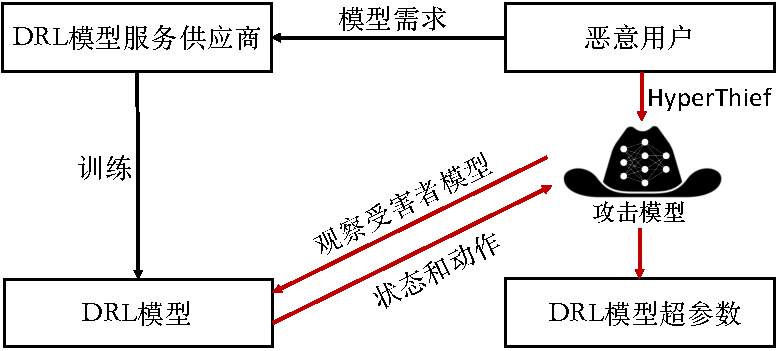
\includegraphics[width=0.6\hsize]{figure/drl_hypertheif/fig-drl-systemch.pdf}
    \caption{本文算法应用场景}
    \label{fig:application scenario}
\end{figure}
\subsection{攻击者能力假设}
我们考虑一个对受害者DRL模型具有黑盒访问权限的攻击者,这是最符合实际情况的情景。
当受害者DRL模型与环境交互时,攻击者可以观察其状态和动作。
另外,攻击者可以将受害者DRL模型部署在自己构建的环境中,因此攻击者可以在合法范围内调整环境状态。
本章主要评估模型超参数的泄露风险,对于DRL模型所使用框架的泄露风险,
可以基于文献{\rm\parencite{CGZXL21}}所提方法进行评估。
% 实际上,攻击者可以计算平均累计奖励以估计受害者的奖励标准(性能)从模型与环境的交互中。例如,如果DRL模型经过多个周期后的平均累计奖励为300,则该模型的奖励标准为300。

\subsection{攻击目的}
% 攻击者旨在推断DRL模型的超参数设置,
攻击者的目标是以较高的准确率推断受害者DRL模型所使用的超参数设置,例如精准判断模型的非线性激活函数和优化器的类型。

\subsection{攻击场景}
\autoref{fig:application scenario} 描述了一个典型的应用场景,
即DRL模型服务供应商训练了一个DRL模型,然后提供API给用户使用。
一个恶意用户想要从受害者DRL模型中推断出超参数设置,
以窃取知识产权或将其作为攻击其他顾客模型的基础。


\section{本文方法(\sysname)}
\subsection{工作流程}
\label{sec:workflow}
\begin{figure*}[!ht]
    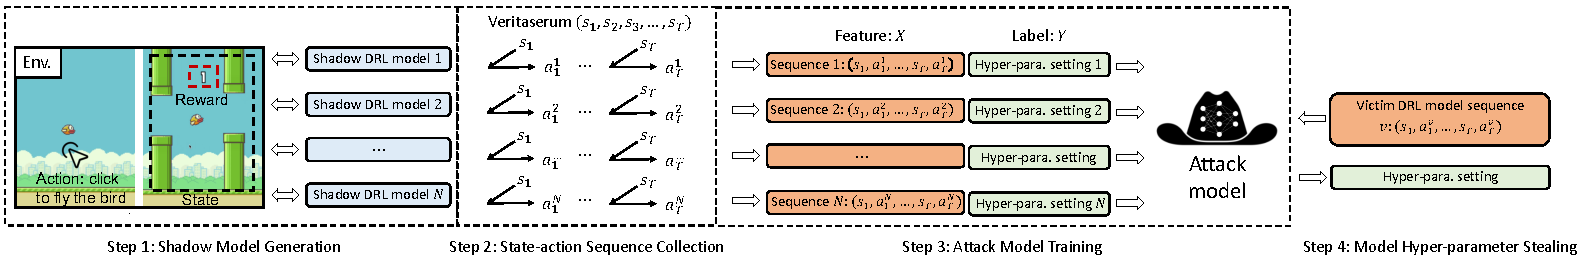
\includegraphics[width=\hsize]{figure/drl_hypertheif/fig-overview-v3.pdf}
    \caption{\sysname 算法主要由四个步骤组成:阴影模型生成、状态-动作序列收集、攻击模型训练和模型超参数窃取。
    \sysname 基于受害者DRL模型的状态和动作中推断其超参数设置。
        % Workflow of \sysname. The four steps in the \sysname algorithm, \ie, shadow model generation, state-action sequence collection, attack model training, and model hyper-parameter stealing. \sysname infers the policy network information from the state and action of the victim DRL model.
    }
    \label{fig:inferring the policy network information}
\end{figure*}

在\autoref{fig:inferring the policy network information}中,
我们以训练DRL模型玩Flappy Bird游戏环境作为例子,
来详细说明DRL超参数推断的工作流程。

\mypara{第一步:阴影模型生成}
在\autoref{fig:inferring the policy network information}的左虚线框中,
攻击者利用Flappy Bird环境生成一组具有不同超参数组合的阴影DRL模型集合。
例如,为了窃取受害DRL模型的激活函数,
攻击者需要训练一组使用不同种类的激活函数的阴影DRL模型。

\mypara{第二步:状态-动作序列收集}
在第二个虚线框中,阴影DRL模型观测环境状态并做出动作。
具体来说,在阴影DRL模型和环境交互过程中,
攻击者记录每个阴影DRL模型的接收的环境状态$s_t$和动作$a^{n}_{t}$,
其中$a^{n}_{t}$表示第$n$个DRL模型在第$t$步的动作。
基于阴影DRL模型动作的差异,
攻击者可以从状态-动作序列中推断出阴影DRL模型的超参数信息。
% 直观地说,攻击者会在收集的状态-动作序列长度越长时,发现更多模型行为的差异。
% 因此,在\autoref{sec:ablation study}中,我们也使用不同长度的状态-动作序列来评估盗取效果。

\mypara{第三步:攻击模型训练}
在完成前两步之后,攻击者获得了一组状态-动作序列以及相应的超参数设置。
对于所有状态-动作序列,攻击者将每一步的状态和动作拼接成一个$(|s|+|a|)$维的特征向量。
这些特征向量沿时间维度拼接成一个$T \times (|s|+|a|)$维的特征矩阵$x$,攻击者得到一个带有超参数设置标签集$Y$的特征集$X$。
然后,可以使用监督分类器(攻击模型)来拟合特征$X$和标签$Y$之间的关系。
攻击模型的目标函数是
\begin{equation}
    \min _{\theta} \underset{x \sim \mathcal{X}}{\mathbb{E}}\left[
        \mathcal{L}\left(f_{\theta}^{p}\left(\left[x\right]_{i=1}^{n}\right), y^{p}\right)\right]\text{,}  
\end{equation}
\mypara{第四步:模型超参数窃取}
攻击者构造状态$s_t$并记录受害者模型的对应行动$a^{v}_t$。
经过第三步的状态和动作预处理之后,攻击者将状态-动作特征输入攻击模型,获得超参数预测结果。

在其他设置不变的情况下,不同的状态$s_t$会导致推断精度的差异。
例如,当小鸟的位置低于障碍物时,所有影子DRL模型都采取了相同的动作,那么攻击模型将无法从状态-动作序列中获得任何模型超参数的信息。
相反,如果攻击者构造的状态能够刺激DRL模型产生更多的行为分歧,攻击模型的推断将更加有效。



\subsection{攻击状态构造}
\label{sec:attack state generation}
在攻击过程中,状态序列在推断受害模型的超参数设置方面起着重要作用。
接下来,我们介绍两种状态构造方法。
\begin{algorithm}[!t]
    \caption{状态扰动}
    \label{alg:state perturbation}
    \begin{algorithmic}[1]
    \REQUIRE 环境 $E$, 状态 $s$
    \ENSURE 扰动后的状态 $s^{\prime}$
    \STATE $//$ 获得环境状态的合法取值范围 of $E$
    \STATE low\_bound, high\_bound = $E$.spaces.Box()
    \STATE $//$ 限制扰动噪声的幅值
    \STATE low\_bound, high\_bound = $\frac{\text{low\_bound}}{10}$, $\frac{\text{high\_bound}}{10}$
    \FOR {$i$-th dimention in $E$.spaces}
    \STATE ${\sigma}$ = min$\left(\lvert\text{low\_bound}\rvert, \lvert\text{high\_bound}\rvert\right)$
    \WHILE {True}
    \STATE $//$ 判断扰动后的状态是否在合法取值范围
    \STATE $s^{\prime}$[$i$] = $s$[$i$] + $N\left(0, {\sigma}^2 \right)$
    \IF {$s^{\prime}$[$i$] in $E$.spaces.Box(dim=$i$)}
    \STATE break
    \ENDIF
    \ENDWHILE
    \ENDFOR
    \STATE 返回 $s^{\prime}$
    \end{algorithmic}
\end{algorithm}


\mypara{被动状态构造机制}
\begin{algorithm}[!t]
    \caption{被动状态构造方法}
    \label{alg:Generation Mechanism 1}
    \begin{algorithmic}[1]
    \REQUIRE Shadow DRL models $M$, environment $E$, the max time step $T$
    \ENSURE State sequence $S = {s_1, s_2, ..., s_T}$
    \STATE Randomly select a DRL model with policy $\pi_{\theta}$
    \STATE Let $S = \{\}$
    \STATE Initialize $E$ randomly with $s_0$ and done\_signal = False
    % \STATE done_signal = False
    \FOR {time step $t$ from $1$ to $T$}
    \IF {done\_signal == True}
    \STATE $s_0^{\prime}$ = \autoref{alg:state perturbation}~($E$, $s_0$)
    \STATE Re-initialize $E$ randomly with $s_0^{\prime}$
    \STATE $//$ Get the action from the DRL model
    \STATE $a_t = \underset{a \in \mathbb{A}}{\arg \max \text{}} \pi_{\theta}(s_0^{\prime}, a) $
    \ELSE
    \STATE $a_t = \underset{a \in \mathbb{A}}{\arg \max \text{~}} \pi_{\theta}(s_{t-1}, a) $
    \ENDIF
    \STATE $//$ Get the new state $s_t$ and the game over signal
    \STATE $s_t, \text{done\_signal} = E(a_t) $
    \STATE Insert the $s_t$ into $S$
    \ENDFOR
    \STATE Return $S$
    \end{algorithmic}
\end{algorithm}
获取状态序列的一种直观方法是直接从影子深度强化学习模型与环境的交互中收集。
\autoref{alg:Generation Mechanism 1} 显示了详细的状态生成过程。
攻击者随机选择一个带有策略$\pi_{\theta}$的深度强化学习模型,然后使用状态空间中的任意$s_0$初始化环境。
例如,在flappy bird游戏中,位于小鸟位于屏幕中央是一个有效状态。
DRL模型将$s_0$放入策略网络$\pi_{\theta}$,然后获取动作$a_1$。
环境转移到下一个状态$s_1$,并判断游戏是否结束。
攻击者将$s_1$插入状态序列$S$中。如果$\text{done\_signal}$是$\text{True}$,则$s_t$是环境的终止状态。
攻击者检查时间步$t$是否等于达到最大步长$T$,
如果$t<T$,攻击者通过\autoref{alg:state perturbation} 生成一个新的初始状态$s^{\prime}_0$,并重新初始化环境。
然后,攻击者继续收集状态,直到时间步长达到$T$。
如果状态维度之间存在物理约束,
我们只需使用\autoref{alg:state perturbation} 扰动部分维度,并通过约束获得其余维度。

被动方法是一种有效的生成状态序列的策略。
然而,它也存在两个缺陷:
1) 没有充分利用白盒影子模型,例如白盒模型的模型权重、更新梯度信息;
2) 攻击模型容易因为静态状态序列而在影子模型上过拟合。


\mypara{主动状态构造机制}
\begin{algorithm}[!t]
    \caption{主动状态构造机制}
    \label{alg:Generation Mechanism 2}
    \begin{algorithmic}[1]
    \REQUIRE 影子模型集合 $M$, 环境 $E$, 最大步长 $T$, 超参数设置集合 $Y$, 攻击模型 $f_{\theta}^{p}$
    \ENSURE 优化后的状态 $S = \{s_1, s_2, ..., s_T\}$
    \STATE $//$ 获取初始状态
    \STATE $S$ = \autoref{alg:Generation Mechanism 1}~($M$, $E$, $T$)
    \STATE state\_update = False
    \FOR {epoch $i$ from $1$ to $n$}
    % \State $//$ BUILD FEATURE MATRIX SET $X$ AND HYPER-PARAMETER SETTING LABEL SET $Y$ BASED ON STEP 2 AND STEP 3 IN \autoref{sec:workflow}
    \IF {$i$ \% $m$ == 0 and state\_update == False}
    \STATE $f_{\theta}^{p}$.loss = $f_{\theta}^{p}$.loss\_calculation($X$, $Y$)
    \STATE $//$ 更新$S$
    \STATE 基于$f_{\theta}^{p}$.loss 反向传播来优化 $S$
    % \State BUILD THE NEW FEATURE SET $X^{\prime}$, AND LET $X=X^{\prime}$
    \STATE state\_update = True
    \ENDIF
    \IF {$i$ == 1 or state\_update == True}
    \STATE $//$ 记录影子模型的动作
    \STATE $X$ = []
    \FOR {$M$中的第$j$个影子模型}
    \STATE $\{a_1, a_2, ..., a_T\}_j$ = $M[j](S)$
    \STATE $X$.append(concatenate($\{a_1, a_2, ..., a_T\}_j$, $S$))
    \STATE 将$X$转化为tensor
    \ENDFOR
    \STATE state\_update = False
    \ENDIF
    \STATE $//$ 更新攻击模型
    \STATE $f_{\theta}^{p}$.train($X$, $Y$)
    \ENDFOR
    \STATE 返回 $S$
    \end{algorithmic}
\end{algorithm}
攻击者利用阴影深度强化学习模型的梯度来生成更有效的状态序列,即主动状态生成方法。
由于阴影深度强化学习模型是白盒的,攻击者可以访问其超参数设置和策略网络中的梯度信息。
与静态状态序列的 \autoref{alg:Generation Mechanism 1} 相比,
\autoref{alg:Generation Mechanism 2} 在攻击模型的训练过程中更新状态序列,即动态状态序列。
我们在训练攻击模型时优化状态以最小化模型损失函数,从而加强状态-动作序列与超参数之间的关系。
\begin{equation}
    \min _{S} \underset{M \sim \mathcal{M}}{\mathbb{E}}\left[ \mathcal{L}\left(f_{\theta}^{p}\left(\left(S, M\left(S\right)\right)\right), y^{p}\right)\right], 
\end{equation}
其中,$S$是状态序列,$\mathcal{M}$是DRL阴影模型集合,$y^{p}$是超参数$p$的真实标签,$\mathcal{L}$是交叉熵损失。
如\autoref{alg:Generation Mechanism 2}第8行所示,
在训练过程中,攻击模型$f_{\theta}^{p}$的损失会在每$m$步反向传播以优化状态序列$S$。
攻击者基于更新后的状态序列$S$重建一个新的特征集$X$,然后使用$X$和$Y$训练分类器,直到下一个状态更新。
攻击者使用最新的状态序列从受害者DRL模型中收集动作,进行超参数推断。

\subsection{讨论}
\begin{figure}[!h]
    \centering
    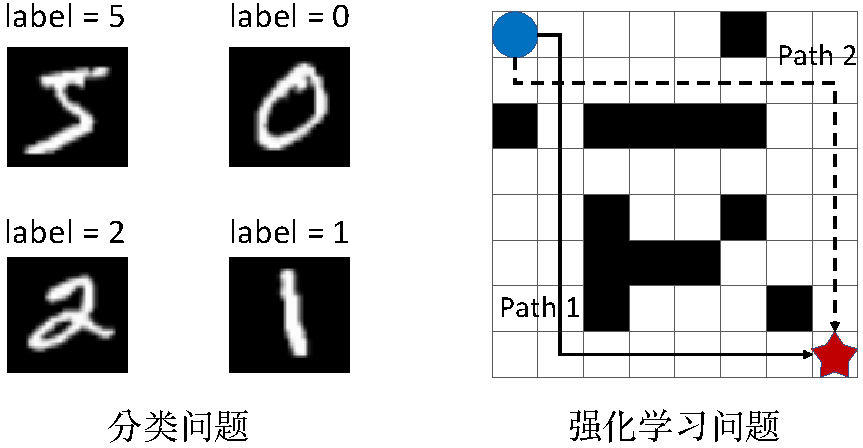
\includegraphics[width=0.6\hsize]{figure/drl_hypertheif/fig-drl-challengech.pdf}
    \caption{针对强化学习模型进行超参数推断攻击中的新挑战。与分类中的显式标签相比,强化学习问题通常有许多等效策略,即最优策略的非唯一性。
    例如,路径1和路径2都是最短路径,这会对推断攻击的造成干扰。} 
    % \mc{I suggest using a shallow grid color to observe the different actions easily.}}
    \label{fig:drl-challenge}
\end{figure}

\sysname 与文献{\rm\parencite{OASF18}}中的逆向工程策略具有相似之处,即一种用于图像分类器模型的超参数推断方法。
文献{\rm\parencite{OASF18}}的逆向工程策略也具有以下特点:
1)从一系列查询中推断出DNN模型的内部信息,
2)生成更有效的输入以增强对黑盒模型超参数的推断精度。
然而,\sysname 在几个关键方面与文献{\rm\parencite{OASF18}}不同,这些差异主要是因为这两种方法针对的受害模型不同。
文献{\rm\parencite{OASF18}}是针对DNN框架下的图像分类器模型,而\sysname 适用于序列决策制定的DRL模型。

\begin{itemize}
    \item \mypara{缺乏良好的数据集}
    与DNN训练场景不同,Oh等人~\cite{OASF18}可以使用训练样本作为高质量的查询输入,而DRL模型则是从环境的交互中进行学习。
    因此,在攻击之前\sysname 没有现成的查询输入。
    我们需要根据训练好的阴影模型构建状态。
    \item \mypara{序列决策任务} 
    文献{\rm\parencite{OASF18}}通过一个单独的查询输入来从DNN模型中提取信息,即通常在每个步骤中处理一个图像样本。
    由于DRL模型是为了优化累积回报而设计的,每个步骤中包含的内部信息是有限的(回顾\autoref{sec:Reinforcement Learning Problem})。
    因此,\sysname 需要构建一系列状态来推断模型超参数。
    \item \mypara{新的超参数} 
    除了文献{\rm\parencite{OASF18}}探究的超参数外,\sysname 还考虑了DRL的特有超参数,即折扣因子$\gamma$。
    \item \mypara{最优策略的非唯一性} 
    如\autoref{fig:drl-challenge}所示,\sysname 在DRL情景中面临新的挑战。
    对于分类问题,每个样本只有一个正确的标签。
    然而,在RL问题中通常存在多个最优策略,这会对推断准确性造成干扰。
\end{itemize}

\section{性能评估}
\label{sec:evaluation}
在本节,我们在三种深度强化学习模型DQN、PG和PPO,以及两个Gym~\cite{BCPSSTZ16}环境CartPole和Acrobot验证\sysname 的有效性。
这些模型和环境在现有研究~\cite{WJWGXS21,CGZXL21,PWZLYS19,GDWKLR20,WGWX21}中被广泛使用。
通过实验评估,我们计划回答下列问题。

\begin{itemize}
    \item 问题 1:能否通过 DRL 模型的行为推断出其超参数设置?
    \item 问题 2:哪种状态更有利于推断出超参数设置?
    \item 问题 3:其他实验因素,例如受害者 DRL 模型的性能、超参数耦合、状态-动作序列的长度以及阴影DRL模型的数量,如何影响攻击?
    \item 问题 4:是否有防御方法可以有效抵御\sysname ?
\end{itemize}

\subsection{环境}
\label{subsec:environments}

我们选择了 Gym 中的“CartPole”环境,该环境同样被其他最新的DRL模型窃取攻击的工作采用~\cite{CGZXL21}。
除了“CartPole”,我们还在“Acrobot”环境上评估所提方法。
我们基于这些环境评估 \sysname 的性能,
并证明了所提方法在不同 DRL 模型和环境中的有效性。
我们认为这些环境是具有代表性的:
1)Gym 环境是主流开源研究平台之一,其提供了统一的接口来训练和测试 DRL 模型;
2)所选的两个环境常用于评估针对 DRL 模型的攻击的有效性~\cite{CGZXL21,IUQJAHN20,PTLBC18}。

\subsection{实验设置}
\label{sec:experimental setup}
\mypara{DRL模型}
我们在 DQN、PG 和 PPO 模型上评估了 \sysname 。
这三个模型代表了 RL 模型的三种基本思想,即基于值的强化学习模型、基于策略更新的强化学习模型和Actor-Critic强化学习模型。
% 大多数现有的无模型 RL 方法都是从这三种方法演变而来的。
DQN 和 PG 通常作为复杂 DRL 模型的基础模块,
PPO 模型代表着最新的DRL模型。
因为卓越的模型性能和训练收敛性,PPO被OpenAI设置为默认的DRL模型,并在现有文献中广泛使用~\cite{WJWGXS21,CGZXL21,GDWKLR20,WGWX21}。

\mypara{目标超参数}
如\autoref{tab:hyper-parameter settings}所示。
表中前三个超参数涉及深度强化学习策略网络架构,
其他超参数与模型优化过程有关。
对于每个超参数,我们选择了三个不同的值。
这些值通常是开源框架(如Baselines和Stable-baselines)的默认选择,例如优化器选项中的ReLU和Adam。

\mypara{影子模型构造}
我们考虑三个DRL模型(DQN,PG和PPO)和两个Gym环境(CartPole和Acrobot)的六种实验组合。
对于每种实验组合,我们在每个超参数设置下训练20个影子DRL模型(共$20\times3^6$个)。
然后,我们将这些影子模型按照4:1分成一个训练模型集合($16\times3^6$)和一个测试模型集合($4\times3^6$)。
由于在某些超参数设置下很难训练出和受害者模型性能相同的影子模型\cite{MBMGLHSK16},
因此\autoref{tab:hyper-parameter settings}中的超参数分布在影子DRL模型集合中是不均匀的。

\mypara{性能指标}
我们使用超参数设置的预测准确性来评估推断攻击的效果\cite{PWZLYS19,CGZXL21,OASF18}。
具体来说,我们利用训练模型集合中的影子模型生成状态-动作序列并训练攻击模型。
然后,我们将测试模型集合中的影子模型作为受害模型,并基于状态-动作序列推断其超参数设置。

\mypara{对比方法}
我们比较了被动和主动状态构造方法的推断性能差异。
其中,“passive\_env”(\autoref{alg:Generation Mechanism 1})直接使用DRL模型和环境之间的交互得到的状态。
“active\_env”在“passive\_env”构造状态的基础上,利用\autoref{alg:Generation Mechanism 2}对状态执行进一步的优化。
在实验中,这两种方法的默认序列长度为200。
基线方法“majority\_vote”采用影子模型集合中比例较大的超参数设置作为推断结果。

\mypara{攻击模型设置}
我们基于ResNet框架构造攻击模型,其具体结构如\autoref{tab:structure of attack model}所示。
我们对攻击模型进行400个epoch的训练。
对于被动方法,我们使用学习率为0.01的SGD优化器来训练攻击模型。
对于主动方法,我们在攻击模型训练期间每10个epoch使用学习率为0.01的Adam优化器来优化状态。

\begin{table}[!t]
    \caption{攻击模型的网络结构。
    在每个卷积层中,$K_c$(核大小)从7变为3。
    $C_o$是输出通道数,变量\textit{stride}是互相关步长。
    $L_{out}$是AdaptiveAvgPool函数的输出向量长度。
    % \mc{If the space is limited, put this table to appendix.}
    }
    \label{tab:structure of attack model}
    \centering
    \resizebox{0.5\linewidth}{!}{
    \setlength{\tabcolsep}{0.8em}
    \begin{tabular}{cc}
    \toprule
    \textbf{Layer Name} & \textbf{Hyper-parameter}                    \\ \toprule
    \textbf{Conv1\_x}            & $K_c=7, 5, 3$, $C_o=64$, $\text{stride}=1$  \\
    % \rowcolor{mygray}
    \textbf{Conv2\_x}            & $K_c=7, 5, 3$, $C_o=128$, $\text{stride}=1$ \\ 
    \textbf{Conv3\_x}            & $K_c=7, 5, 3$, $C_o=128$, $\text{stride}=1$ \\
    % \rowcolor{mygray}
    \textbf{AdaptiveAvgPool}     & $L_{out}=\text{sequence length}$            \\
    \textbf{Relu}                & -                                           \\
    % \rowcolor{mygray}
    \textbf{Linear\_1}           & $(C_o \times L_{out}, L_{out})$             \\ 
    \textbf{Linear\_2}           & $(L_{out}, \text{\#classes})$               \\
    % \rowcolor{mygray}
    \textbf{Softmax}             & dim=1                                       \\ \bottomrule
    \end{tabular}
    }
\end{table}
% 超参数值的分布情况在\autoref{sec:the distributions of hyper-parameter}中给出。

\mypara{实验部署平台}
我们使用Tianshou库\cite{weng2021tianshou}来实现所有DRL模型。
所有攻击方法采用Python 3.7实现,并在NVIDIA DGX-A100服务器上运行。

\subsection{总体性能}
\label{sec:overall performance}
\mypara{实验设置}
受害者DRL模型在与环境的一回合交互中能够获取的累计奖励分别为500(Cartpole)和-100(Acrobot)。
在\autoref{fig:overall performence}中,
x轴展示了不同的超参数类型,y轴展示了相应的推断准确性。
每个直方图展示了在三次重复实验中推断准确率的平均值和标准差。

\begin{figure*}[!ht]
    \centering
    \subfigure[DQN, CartPole, Reward = 500]{
    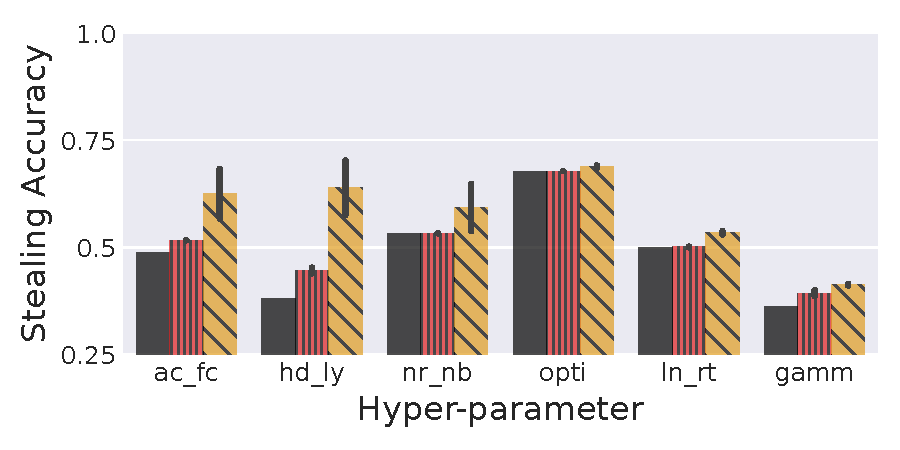
\includegraphics[width=0.3\hsize]{figure/drl_hypertheif/overall_acc/dqn-cartpole-reward500-20220731.pdf}
    \label{fig:DQN CartPole 500 all}
    }
    \subfigure[PG, CartPole, Reward = 500]{
    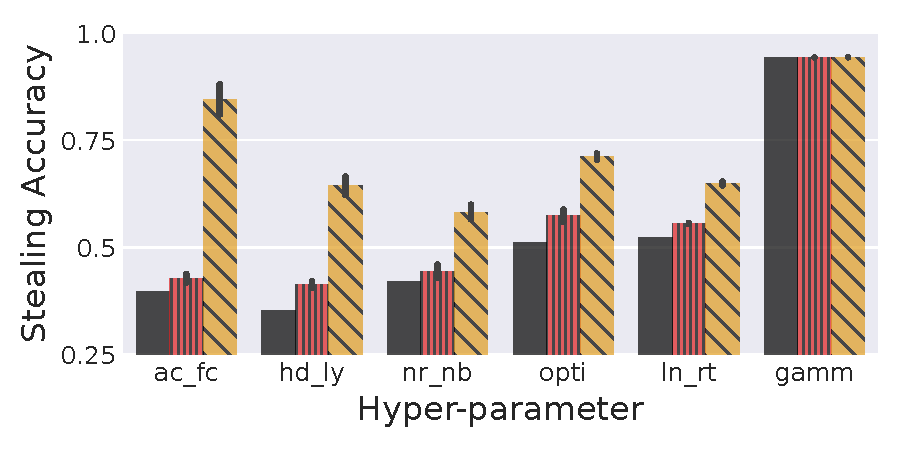
\includegraphics[width=0.3\hsize]{figure/drl_hypertheif/overall_acc/pg-cartpole-reward500-20220731.pdf}
    \label{fig:PG CartPole 500 all}
    }
    \subfigure[PPO, CartPole, Reward = 500]{
    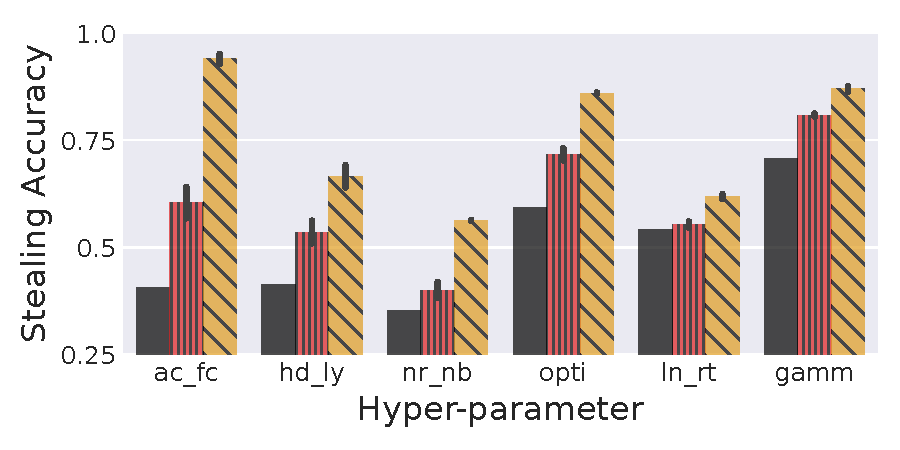
\includegraphics[width=0.3\hsize]{figure/drl_hypertheif/overall_acc/ppo-cartpole-reward500-20220731.pdf}
    \label{fig:PPO CartPole 500 all}
    }
    \\[-2ex]
    \subfigure[DQN, Acrobot, Reward = -100]{
    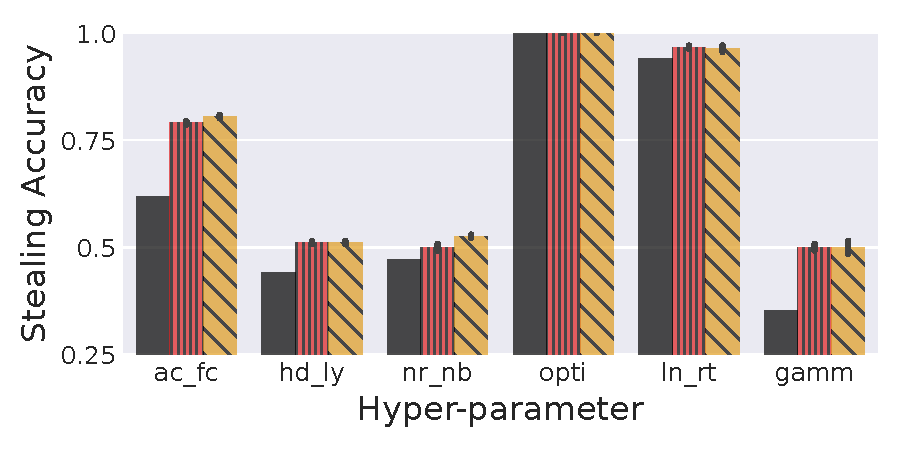
\includegraphics[width=0.3\hsize]{figure/drl_hypertheif/overall_acc/dqn-acrobot-reward0100-20220731.pdf}
    \label{fig:DQN Acrobot -100 all}
    }
    \subfigure[PG, Acrobot, Reward = -100]{
    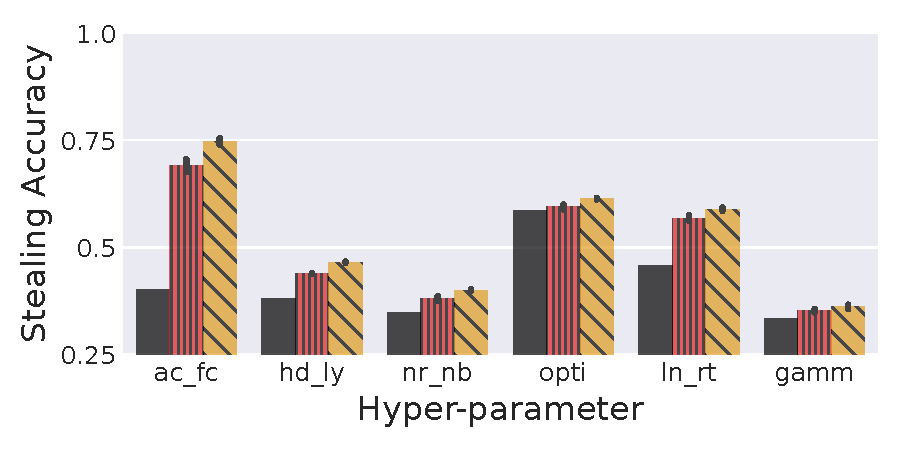
\includegraphics[width=0.3\hsize]{figure/drl_hypertheif/overall_acc/pg-acrobot-reward0100-20220731.pdf}
    \label{fig:PG Acrobot -100 all}
    }
    \subfigure[PPO, Acrobot, Reward = -100]{
    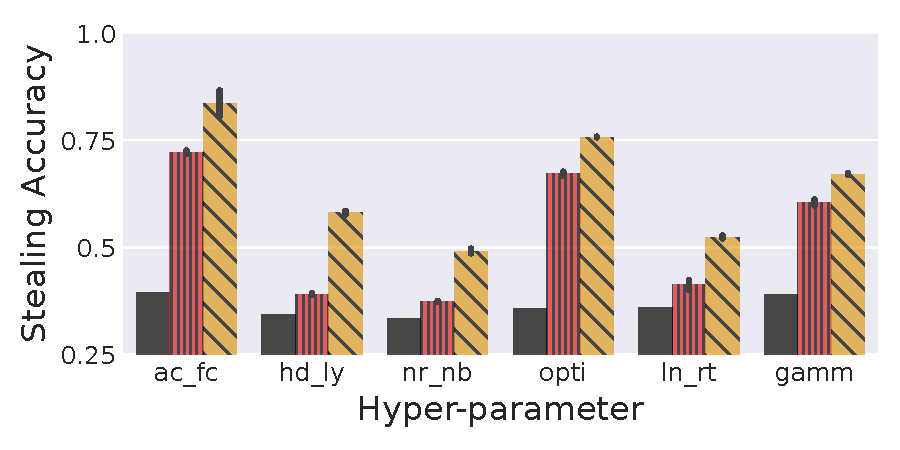
\includegraphics[width=0.3\hsize]{figure/drl_hypertheif/overall_acc/ppo-acrobot-reward0100-20220731.pdf}
    \label{fig:PPO Acrobot -100 all}
    }\\[-0.5ex]
    \subfigure{
\includegraphics[width=0.4\textwidth]{figure/drl_hypertheif/overall/overall-legend-20220731.pdf}} 
    % \subfigure{
    % 
\includegraphics[width=0.65\hsize]{figure/drl_hypertheif_others/comparison_1D_legend6.pdf.pdf} 
    % }
    \vspace{-0.4cm}
    \caption{不同方法在DRL模型和环境六种组合上的超参数推断准确性。
    每个图的x轴标签依次对应于激活函数、隐藏层、神经元数、优化器、学习率和gamma超参数。
    y标签显示推断准确率。
    % \mc{This figure is the most important figure, make it as clear as possible.
    % Make the fontsize larger, add one sentence to explain the reward numbers. I am not sure whether ``-100'' is the highest reward?}
    % \mc{Check the name of each method, keep them consistent in the whole paper, including the figures and captions. Check whether the values are consistent with the conclusions. }
    }
    % \vspace{-0.2cm}
    \label{fig:overall performence}
\end{figure*}

\mypara{实验结果}
我们从\autoref{fig:overall performence}总结出以下结论。
1)\sysname 的窃取精度都高于majority\_vote方法,这意味着DRL模型的行为确实可以暴露模型的超参数设置。
例如,激活函数的推断精度超过了60%,在PPO上甚至超过了90%。
2)\sysname 在不同的 DRL 模型上推断准确率不同。
对于优化器和学习率,攻击者在 PG 和 PPO 模型上的推断效果优于 DQN 模型。
如 \autoref{fig:PG CartPole 500 all} 和 \autoref{fig:PPO CartPole 500 all},\sysname 在优化器和学习率上取得了巨大的准确率提升,而在 \autoref{fig:DQN CartPole 500 all} 中略微超过了基线方法。
回顾 \autoref{sec:Deep Reinforcement Learning model},DQN 模型在训练过程中使用策略网络来近似$\mathcal{Q}$表,并根据形成的$\mathcal{Q}$表选择动作,即状态是通过影响Q值进而决定行为动作。
PG 和 PPO 则使用策略网络直接建立状态和动作之间的关系,而不是像 DQN 中那样近似$\mathcal{Q}$表,即状态直接决定行为动作。
因此,从 DQN 中推断出与优化相关的超参数更为困难。
3)从\autoref{fig:overall performence}中可以看出,\sysname 对于不同的超参数具有不同的盗取准确度。
通常情况下,\sysname 在激活函数上的推断准确度要高于学习率。
作为结构超参数,不同的激活函数具有独特的特征。
例如,Tanh激活函数在$(0,0)$处对称,而ReLU和ELU激活函数是不对称的。
此外,激活函数的功能特征在构建DRL模型后不会改变,因此激活函数的推断准确性在DRL模型和环境的组合上保持良好性能。
对于学习率,它控制着模型权重的更新速度。
相对于激活函数而言,学习率通过影响模型的权重值来引导模型的行为。
因此,学习率的特征在随着模型训练会变得难以推断。

\subsection{受害者模型性能的影响}
\label{sec:impact of model reward}
\begin{figure*}
    \centering
    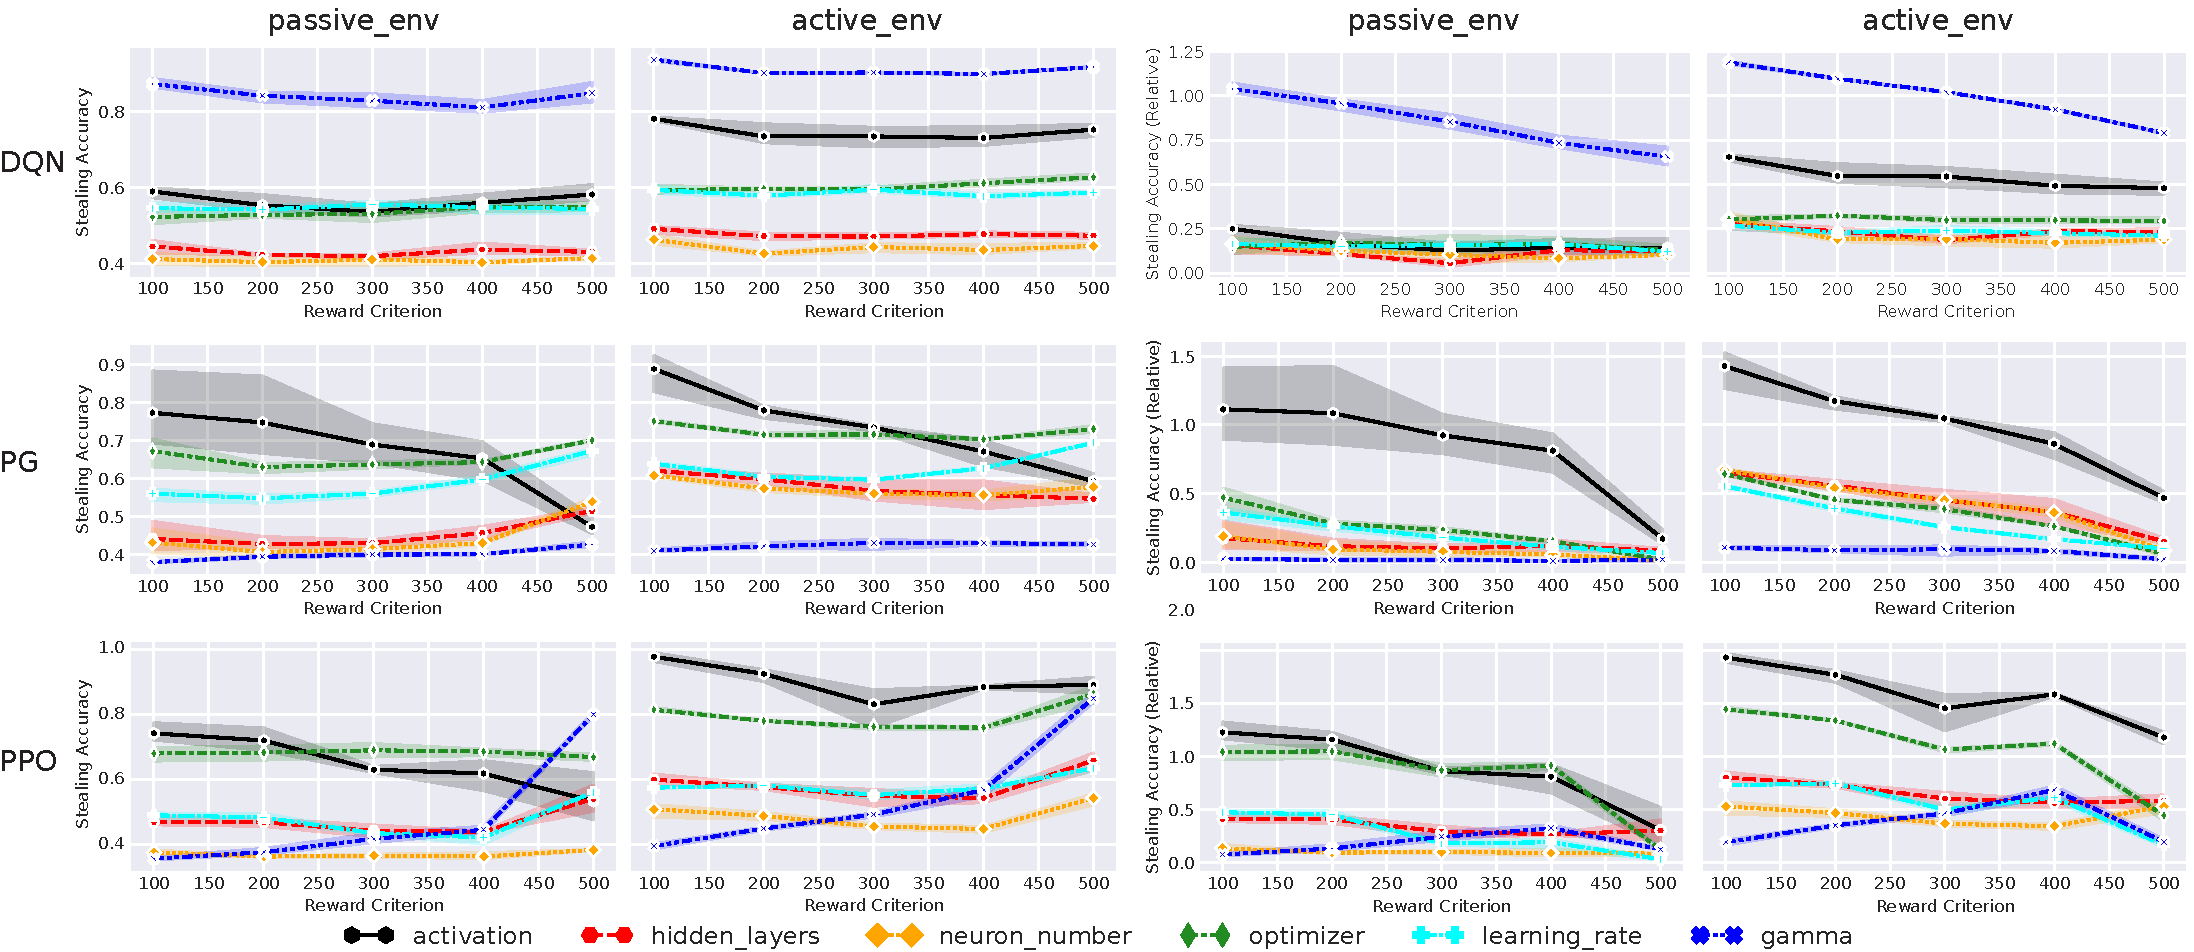
\includegraphics[width=\hsize]{figure/drl_hypertheif/agent_reward/agent_reward.pdf}
    \caption{
    % The stealing accuracy on three models and the CartPole environment when varying the reward criteria of the victim. 
    % The x labels show the reward criterion of the victim model. 
    % The y labels show the stealing accuracy.
    % The left six plots show the absolute stealing accuracy, and the right six plots show the relative stealing accuracy.  
    在不同受害者模型性能情况下,所提方法在三个模型框架上的推断准确率。
    x轴展示了受害者模型性能(累计奖励),
    y轴展示了所提方法的推断准确率。
    左侧六个图为绝对推断准确率,
    右侧六个图为相对于基线方法“majority\_vote”推断准确率。
    } 
    % \mc{Maybe this is not necessary. If possible, keep the hyparparameter order same in all figures. Otherwise, the line colors might not consistent.}} 
    \label{fig:impact of model reward}
    % \vspace{-0.2cm}
\end{figure*}
我们研究了受害者模型性能和超参数泄露风险之间的关系。

\mypara{实验设置}
基于CartPole环境,我们探究受害者模型的累计奖励从100到500变化时\sysname 推断准确性的变化。
推断准确性受到两个因素的影响。
一方面,随着累计奖励的提高,能够达到该条件的可行超参数设置会减少,这相当于变相降低了推断的难度。
从文献{\rm\parencite{MBMGLHSK16}}中可知,DRL模型对超参数的选择较为敏感。
例如,A3C模型以接近$10^{-3}$的学习率在五个游戏中获得最高分数\cite{MBMGLHSK16}。
另一方面,当累计奖励标准提高时,模型的行为偏好往往难以区分,因为获得高累计奖励的策略数量通常是有限的。
例如,所有强化学习策略可能会在迷宫游戏中选择相同的最短路径以获得最高累计奖励。
因此,我们提供了两种类型的结果,即绝对推断准确性和相对推断准确性。
前者反映综合两个方面影响的推断效果,而后者反映DRL模型随着累计奖励标准变化时行为的可区分性变化。
相对推断准确性为$\text{acc}_{rel}=\frac{\text{acc} - \text{acc}_{maj}}{\text{acc}_{maj}}$,其中$\text{acc}$是\sysname 的绝对推断准确性,$\text{acc}_{maj}$是majority\_vote方法的准确性。
$\text{acc}_{rel}$显示了相对于基线方法的\sysname 推测准确性的相对增量。
每个子图标题中标注了所使用的状态构成方法。

\mypara{实验结果}
根据\autoref{fig:impact of model reward},我们可以得出以下观察结果。
1)从绝对的窃取准确度来看,受害者的性能提升趋向于增加超参数泄露的风险。
超参数泄露主要源于模型在较低的累计奖励标准下的行为偏好以及在较高的奖励条件下有限的可行超参数待选集合。
随着累计奖励标准的提高,符合条件的DRL模型超参数会呈现出明显偏向,特别是超参数 gamma。
例如,当累计奖励标准为100时,所有的超参数设置都能够训练出符合要求的PPO模型。
但是,当累计奖励标准提高到500时,绝大多数PPO模型都是采用gamma = 0.99 (71.21\%)或gamma = 0.95 (27.27\%)。
从\autoref{fig:impact of model reward}可得,随着累计奖励标准从100提高到500,大部分超参数种类的相对推断准确性都有所下降。
这意味着随着奖励条件的提高,模型的行为变得更加收敛。
在训练DRL模型时,我们会优化网络权重以接近最优策略。
高奖励条件意味着DRL模型在与环境的互动中具有更强的能力,即更接近最优策略。
因此,它们的策略具有类似的功能,这削弱了模型行为和超参数设置之间的相关性。
2)不同超参数的绝对推断准确度在奖励条件提高时表现出不一致的趋势。
激活函数和优化器的结果相对稳定,其推断准确性在所有奖励条件下均超过75\%。
而隐藏层数、神经元数量和学习率方面的推断准确度则较低。
我们认为激活函数和优化器在策略优化过程中起着更重要的作用,这导致了DRL模型出现明显的行为倾向。
与这些超参数相比,DRL模型对于隐藏层和神经元数量设置的依赖性不强,即在大多数情况下满足拟合策略的复杂度即可。
此外,我们注意到当奖励条件越高时,超参数gamma的推断准确性会提升。
根据\autoref{sec:Reinforcement Learning Problem},折扣因子$\gamma$影响到DRL模型对未来奖励的关注程度。
因此,高质量的策略倾向于选择更大的gamma以实现更长远的策略视野。
3)主动状态构造机制对奖励条件的变化具有较强的鲁棒性。
相比主动状态构造机制,主动状态构造机制的准确率下降得更慢。
例如,主动状态构造机制的激活函数窃取准确率仍然是基线方法的两倍,而被动状态构造机制与基线方法相同。
由于高质量的DRL模型对于环境的刻画程度更好,所以被动状态构造机制很难使DRL模型的行为出现不一致的情况。
而主动方法调整原始环境状态为较为罕见的环境状态,从而使DRL模型更容易产生行为分歧。

\subsection{超参数之间的耦合影响}
\label{sec:impact of hyper-parameter coupling}
\begin{figure*}[!ht]
    \centering
    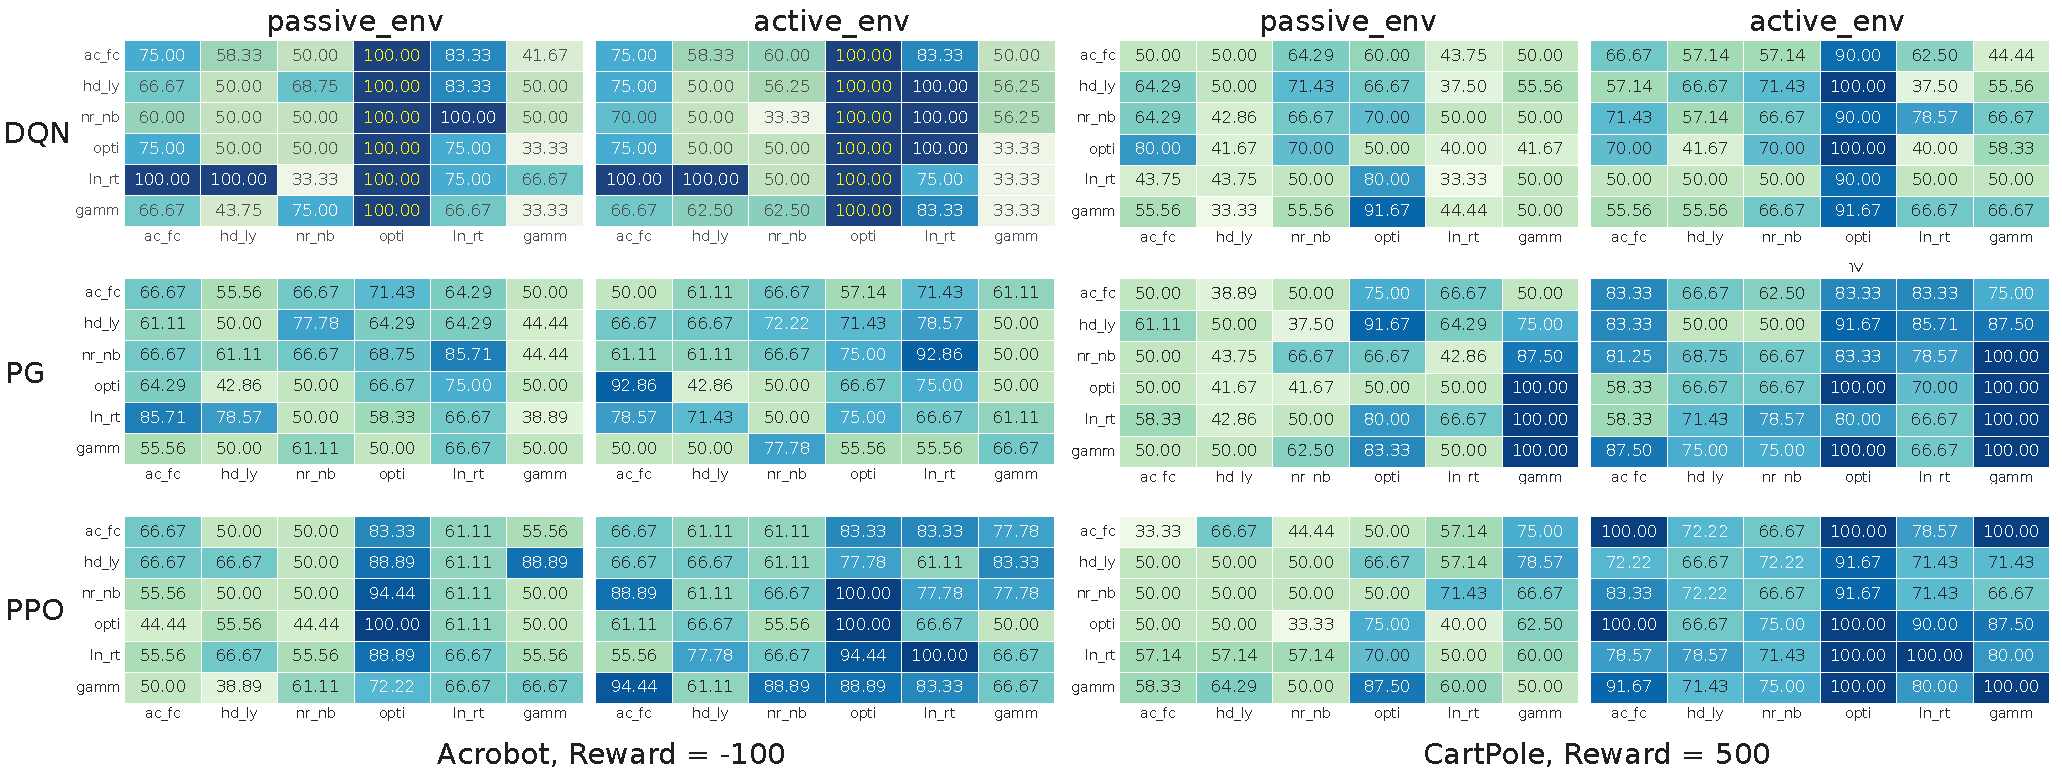
\includegraphics[width=\hsize]{figure/drl_hypertheif/hyper_couple/hyper-couple-2.pdf}
    \caption{
    不同的超参数组合会影响到模型的准确度。
    其中,“passive\_env”和“active\_env”分别表示被动和主动的状态生成机制。
    每个图的x轴标签表示目标超参数,y轴标签表示耦合超参数。
    % The stealing accuracy with different hyper-parameter pairs. 
    % The ``passive\_env'' and ``active\_env'' illustrate the passive and the active state generation mechanisms. 
    % The x labels of each plot show the target hyper-parameters. 
    % The y labels of each plot show the irrelevant hyper-parameters. 
    }
    \label{fig:hyper_couple}
\end{figure*}

% \begin{table}[!ht]
%     \centering
%     \footnotesize
%     \caption{Acrobot 中阴影模型的超参数分布。}
%     \label{Acrobot-reward500-hyperparameter-ratio}
%     \begin{tabular}{cccc}
%     \toprule
%     \multicolumn{4}{c}{\multirow{2}{*}{\textbf{DQN, Acrobot, Reward=-100}}}  \\
%     \multicolumn{4}{c}{}                                            \\ \toprule
%     activation     & ELU: 61.76     & Tanh: 38.24   & NaN           \\
%     hidden\_layers & 4: 44.12       & 3: 32.35      & 2: 23.53      \\
%     neuron\_number & 256: 47.06     & 128: 32.35    & 64: 20.59     \\
%     optimizer      & SGD: 100.00    & NaN           & NaN           \\
%     learning\_rate & 0.0001: 94.12  & 0.0005: 5.88  & NaN           \\
%     gamma          & 0.9: 35.29     & 0.95: 35.29   & 0.99: 29.41   \\ \toprule
%     \multicolumn{4}{c}{\multirow{2}{*}{\textbf{PG, Acrobot, Reward=-100}}}   \\
%     \multicolumn{4}{c}{}                                            \\ \toprule
%     activation     & ELU: 40.22     & Tanh: 38.04   & ReLU: 21.74   \\
%     hidden\_layers & 2: 38.04       & 4: 31.52      & 3: 30.43      \\
%     neuron\_number & 128: 34.78     & 256: 32.61    & 64: 32.61     \\
%     optimizer      & RMSprop: 58.70 & Adam: 30.43   & SGD: 10.87    \\
%     learning\_rate & 0.0005: 45.65  & 0.001: 31.52  & 0.0001: 22.83 \\
%     gamma          & 0.9: 33.33     & 0.99: 33.33   & 0.95: 33.33   \\ \toprule
%     \multicolumn{4}{c}{\multirow{2}{*}{\textbf{PPO, Acrobot, Reward=-100}}}  \\
%     \multicolumn{4}{c}{}                                            \\ \toprule
%     activation     & Tanh: 39.51    & ELU: 37.74    & ReLU: 22.75   \\
%     hidden\_layers & 3: 34.22       & 2: 32.98      & 4: 32.80      \\
%     neuron\_number & 128: 33.51     & 256: 33.51    & 64: 32.98     \\
%     optimizer      & RMSprop: 35.63 & Adam: 34.92   & SGD: 29.45    \\
%     learning\_rate & 0.001: 35.98   & 0.0005: 35.45 & 0.0001: 28.57 \\
%     gamma          & 0.99: 38.98    & 0.95: 35.63   & 0.9: 25.40    \\ \bottomrule
%     \end{tabular}
% \end{table}

% \begin{table}[!ht]
%     \centering
%     \footnotesize
%     \caption{CartPole 中阴影模型的超参数分布。}
%     \label{cartpole-reward500-hyperparameter-ratio}
%     \begin{tabular}{cccc}
%     \toprule
%     \multicolumn{4}{c}{\multirow{2}{*}{\textbf{DQN, CartPole, Reward=500}}}  \\
%     \multicolumn{4}{c}{}
%     \\ \toprule
%     activation     & Tanh: 48.68    & ELU: 46.05     & ReLU: 5.26   \\
%     hidden\_layers & 2: 38.16       & 4: 36.18       & 3: 25.66     \\
%     neuron\_number & 256: 53.29     & 128: 32.89     & 64: 13.82    \\
%     optimizer      & RMSprop: 67.76 & Adam: 32.24    & NaN          \\
%     learning\_rate & 0.001: 50.00   & 0.0005: 40.79  & 0.0001: 9.21 \\
%     gamma          & 0.99: 36.18    & 0.95: 32.24    & 0.9: 31.58   \\ \toprule
%     \multicolumn{4}{c}{\multirow{2}{*}{\textbf{PG, CartPole, Reward=500}}}   \\
%     \multicolumn{4}{c}{} 
%     \\ \toprule
%     activation     & ELU: 39.77     & Tanh: 37.50    & ReLU: 22.73  \\
%     hidden\_layers & 2: 35.23       & 3: 34.09       & 4: 30.68     \\
%     neuron\_number & 256: 42.05     & 64: 29.55      & 128: 28.41   \\
%     optimizer      & Adam: 51.14    & RMSprop: 48.86 & NaN          \\
%     learning\_rate & 0.001: 52.27   & 0.0005: 42.05  & 0.0001: 5.68 \\
%     gamma          & 0.99: 94.32    & 0.95: 5.68     & NaN          \\ \toprule
%     \multicolumn{4}{c}{\multirow{2}{*}{\textbf{PPO, CartPole, Reward=500}}}   \\
%     \multicolumn{4}{c}{}
%     \\ \toprule
%     activation     & Tanh: 40.91    & ReLU: 33.33    & ELU: 25.76   \\
%     hidden\_layers & 4: 41.67       & 3: 36.36       & 2: 21.97     \\
%     neuron\_number & 256: 35.61     & 128: 34.09     & 64: 30.30    \\
%     optimizer      & RMSprop: 59.85 & Adam: 40.15    & NaN          \\
%     learning\_rate & 0.001: 54.55   & 0.0005: 43.94  & 0.0001: 1.52 \\
%     gamma          & 0.99: 71.21    & 0.95: 27.27    & 0.9: 1.52    \\ \bottomrule
%     \end{tabular}
% \end{table}
\begin{table}[!ht]
    \centering
    \footnotesize
    \caption{Acrobot 中阴影模型的超参数分布。}
    \label{Acrobot-reward0100-hyperparameter-ratio}
    \begin{tabular}{cccc}
    \toprule
    \multicolumn{4}{c}{\multirow{2}{*}{\textbf{DQN, Acrobot, Reward=-100}}}  \\
    \multicolumn{4}{c}{}                                            \\ \toprule
    激活函数     & ELU: 61.76     & Tanh: 38.24   & NaN           \\
    隐含层数 & 4: 44.12       & 3: 32.35      & 2: 23.53      \\
    神经元数 & 256: 47.06     & 128: 32.35    & 64: 20.59     \\
    优化器      & SGD: 100.00    & NaN           & NaN           \\
    学习率 & 0.0001: 94.12  & 0.0005: 5.88  & NaN           \\
    gamma          & 0.9: 35.29     & 0.95: 35.29   & 0.99: 29.41   \\ \toprule
    \multicolumn{4}{c}{\multirow{2}{*}{\textbf{PG, Acrobot, Reward=-100}}}   \\
    \multicolumn{4}{c}{}                                            \\ \toprule
    激活函数     & ELU: 40.22     & Tanh: 38.04   & ReLU: 21.74   \\
    隐含层数 & 2: 38.04       & 4: 31.52      & 3: 30.43      \\
    神经元数 & 128: 34.78     & 256: 32.61    & 64: 32.61     \\
    优化器      & RMSprop: 58.70 & Adam: 30.43   & SGD: 10.87    \\
    学习率 & 0.0005: 45.65  & 0.001: 31.52  & 0.0001: 22.83 \\
    gamma          & 0.9: 33.33     & 0.99: 33.33   & 0.95: 33.33   \\ \toprule
    \multicolumn{4}{c}{\multirow{2}{*}{\textbf{PPO, Acrobot, Reward=-100}}}  \\
    \multicolumn{4}{c}{}                                            \\ \toprule
    激活函数     & Tanh: 39.51    & ELU: 37.74    & ReLU: 22.75   \\
    隐含层数 & 3: 34.22       & 2: 32.98      & 4: 32.80      \\
    神经元数 & 128: 33.51     & 256: 33.51    & 64: 32.98     \\
    优化器      & RMSprop: 35.63 & Adam: 34.92   & SGD: 29.45    \\
    学习率 & 0.001: 35.98   & 0.0005: 35.45 & 0.0001: 28.57 \\
    gamma          & 0.99: 38.98    & 0.95: 35.63   & 0.9: 25.40    \\ \bottomrule
    \end{tabular}
\end{table}

\begin{table}[!ht]
    \centering
    \footnotesize
    \caption{CartPole 中阴影模型的超参数分布。}
    \label{cartpole-reward500-hyperparameter-ratio}
    \begin{tabular}{cccc}
    \toprule
    \multicolumn{4}{c}{\multirow{2}{*}{\textbf{DQN, CartPole, Reward=500}}}  \\
    \multicolumn{4}{c}{}
    \\ \toprule
    激活函数     & Tanh: 48.68    & ELU: 46.05     & ReLU: 5.26   \\
    隐含层数 & 2: 38.16       & 4: 36.18       & 3: 25.66     \\
    神经元数 & 256: 53.29     & 128: 32.89     & 64: 13.82    \\
    优化器      & RMSprop: 67.76 & Adam: 32.24    & NaN          \\
    学习率 & 0.001: 50.00   & 0.0005: 40.79  & 0.0001: 9.21 \\
    gamma          & 0.99: 36.18    & 0.95: 32.24    & 0.9: 31.58   \\ \toprule
    \multicolumn{4}{c}{\multirow{2}{*}{\textbf{PG, CartPole, Reward=500}}}   \\
    \multicolumn{4}{c}{} 
    \\ \toprule
    激活函数     & ELU: 39.77     & Tanh: 37.50    & ReLU: 22.73  \\
    隐含层数 & 2: 35.23       & 3: 34.09       & 4: 30.68     \\
    神经元数 & 256: 42.05     & 64: 29.55      & 128: 28.41   \\
    优化器      & Adam: 51.14    & RMSprop: 48.86 & NaN          \\
    学习率 & 0.001: 52.27   & 0.0005: 42.05  & 0.0001: 5.68 \\
    gamma          & 0.99: 94.32    & 0.95: 5.68     & NaN          \\ \toprule
    \multicolumn{4}{c}{\multirow{2}{*}{\textbf{PPO, CartPole, Reward=500}}}   \\
    \multicolumn{4}{c}{}
    \\ \toprule
    激活函数     & Tanh: 40.91    & ReLU: 33.33    & ELU: 25.76   \\
    隐含层数 & 4: 41.67       & 3: 36.36       & 2: 21.97     \\
    神经元数 & 256: 35.61     & 128: 34.09     & 64: 30.30    \\
    优化器      & RMSprop: 59.85 & Adam: 40.15    & NaN          \\
    学习率 & 0.001: 54.55   & 0.0005: 43.94  & 0.0001: 1.52 \\
    gamma          & 0.99: 71.21    & 0.95: 27.27    & 0.9: 1.52    \\ \bottomrule
    \end{tabular}
\end{table}

\mypara{实验设置}
在训练攻击模型以推断某个超参数时,其他超参数可能会对目标超参数产生影响。
为了进一步探究超参数两两之间的影响,我们将一个参数设置为目标超参数,选取另一个作为耦合超参数。
在每张子图的对角线,我们展示了不包含耦合超参数的推断结果。
如\autoref{Acrobot-reward0100-hyperparameter-ratio}和\autoref{cartpole-reward500-hyperparameter-ratio}所示,训练得到的DRL模型的超参数分布是不均匀的。
这意味着某些超参数设置下没有满足累计奖励标准的模型。

\mypara{实验结果}
从\autoref{fig:hyper_couple}中,我们可以得出以下结论。
1)超参数对模型行为偏好的影响程度不同。
例如,当优化器是目标超参数时(对应着x轴上的“opti”),推断精度一般是优于其他超参数作为目标参数的情况。
因此,优化器对 DRL 模型的行为影响比其他超参数更强。
此外,超参数 gamma(即x轴上的“gamm”)对三个 DRL 模型具有不同的影响特性。
与 DQN 模型相比,PG 和 PPO 模型的动作更多地暴露了有关 gamma 设置的信息。
回顾\autoref{sec:Deep Reinforcement Learning model},DQN 模型是基于值的RL模型,这意味着 DQN 模型通过比较下一状态的期望累计奖励来选择动作。
而PG 和 PPO 模型直接利用期望累计奖励来更新策略网络,所以模型更新过程中更加依赖累计奖励的数值。
因此,gamma 设置对 PG 和 PPO 模型有更显著的影响。 
2)主动状态构造方法在一定程度上可以解耦不同超参数之间的影响,所以主动状态构造方法的性能比被动状态构造方法更优秀。
例如,当学习率是目标超参数时,由于其他耦合超参数的影响,使用被动状态构造方法的推断准确率约为60\%。
但是,使用主动状态构造方法时,相应的结果可以达到约75\%(甚至100\%)。





\subsection{消融实验}
\label{sec:ablation study}
\begin{figure*}[!t]
    \centering        
    \includegraphics[width=\hsize]{figure/drl_hypertheif/sequence_length/sequence_length-2.pdf}
    \caption{不同状态-动作序列长度下推断准确率的变化。
    每张图的x轴代表用于训练攻击模型的状态-动作序列的长度,y轴显示了相应的推断准确率。
    }
    \label{fig:ablation the length of state-action sequence}
    % \vspace{-0.3cm}
\end{figure*}
\begin{figure*}[!t]
    \centering
    \includegraphics[width=\hsize]{figure/drl_hypertheif/shadow_agent_amount/shadow_agent_amount-2.pdf}
    \caption{不同影子模型数量下推断准确率的变化。每张图的x轴代表用于训练攻击模型的影子模型数量,y轴显示了相应的窃取准确率。
    % \mc{The legend labels are not consistent with \autoref{fig:overall performence}.}
    }
    \label{fig:ablation the amount of shadow models}
\end{figure*}
\mypara{序列长度的影响}
\sysname 在序列长度从短(100步)到长(500步)条件下来进行推断攻击,并比较不同状态生成机制的推断效果。
根据\autoref{fig:ablation the length of state-action sequence},我们得出以下观察结果。
1)较长的状态-动作序列有利于窃取攻击。
在\autoref{fig:ablation the length of state-action sequence}中,随着序列长度的增加,推测准确率往往会上升。
尤其是在CartPole环境中,对于PPO模型的激活函数的推测准确率从53\%上升到70\%。
两种攻击方法都使用DRL模型和环境交互过程的状态-动作数据。
因此更长的序列可能包含更多的行为分歧,有助于进行推断攻击。
2)状态-动作序列的长度对主动状态构造机制的影响较小。
主动状态构造机制的推断准确率几乎不随状态-动作序列长度的变化而变化。
由于优化后的状态序列中的每个状态更有可能使模型的动作不一致,因此主动状态构造机制的基础性能优于被动机制。
在主动状态构造机制中,使用100步状态-动作序列就足以取得和被动机制使用500步状态-动作序列相当的效果。

\mypara{影子模型数量的影响}
我们将训练攻击模型所使用的每个超参数设置下的影子模型数量从4个增加到16个。
根据\autoref{fig:ablation the amount of shadow models},我们得出以下观察结果。
1)随着影子模型数量的增加,窃取准确率会增加。
在训练影子模型时,环境的初始状态和模型的探索过程会给模型的策略带来一定的随机性。
因此,攻击模型可以通过使用来自更加多样化的影子模型的状态-动作序列来降低随机性对于超参数推断的影响。
2)主动攻击方法更有效地利用了影子模型。
回顾\autoref{sec:attack state generation},主动状态生成方法使用攻击模型的损失来优化状态序列,从而可以刺激DRL模型表现出更多的行为分歧。
即使在影子模型数量有限的情况下(例如只有4个影子模型),主动方法仍然可以比被动方法实现更高的超参数推断准确率。

\subsection{案例分析}
\label{sec:case study}
\subsubsection{对抗样本攻击的可迁移性}
泄漏的超参数信息使DRL模型在面对其他攻击时更加脆弱。
例如,模型提取攻击~\cite{TZJRR16}和对抗样本攻击~\cite{HPGDA17, BM17, LHLSLS17, KS17}。
% 对于模型提取攻击,Chen等人~\cite{CGZXL21}提出了第一种方法来窃取黑盒受害者DRL的功能,并确认了超参数和网络结构对识别算法族准确性的影响。
在本节中,我们展示了泄漏的超参数信息对于对抗样本攻击的可迁移性的增益效果。
实验设置与文献{\rm\parencite{CGZXL21}}保持一致,并利用GAIL~\cite{DBLP:conf/nips/HoE16}生成影子模型。
% 因此,以下实验可以用作比较\cite{CGZXL21}和\sysname之间转移增强的实验。

\mypara{实验设置}
我们随机选择了20个具有不同超参数设置的受害者模型,并分别生成了两组具有和不具有超参数信息的$20 \times 8$个影子模型。
对于每个白盒影子模型,我们生成一条长度为500步的对抗状态序列,并将对抗状态序列应用于受害者模型,并记录攻击成功率(对抗状态序列的可迁移性)。
在每个实验设置下,我们重复10次实验,并计算每个影子模型产生的对抗状态序列可迁移性的平均值。
我们展示出所有$20 \times 8$个影子模型中平均可迁移值超过90\%的影子智能体的百分比。
实验使用四种不同的对抗样本生成方法,即FGM、FGSM \cite{DBLP:journals/corr/GoodfellowSS14}、L2PGD和LinfPGD\cite{DBLP:conf/iclr/KurakinGB17a, DBLP:conf/iclr/MadryMSTV18}。

\begin{table}[!t]
    \centering
    \caption{影子模型集合中的平均可转移值超过90\%的模型比例,结果基于 PPO模型 和 CartPole 环境。
        % The percentage of shadow agents with average transferability values more than 90\%. 
    % The results are collected from PPO and the CartPole environment.
    % (\textbf{reward = 300}). 
    % In each table, the `W' and `W/O' illustrate the transferability experiment with or without the hyper-parameters information, and $\epsilon$ controls the strength of adversarial perturbation. 
    }
    \label{tab:adv-transferability-ppo-cartPole-reward300}
    % \resizebox{\textwidth}{5mm}{
    \resizebox{0.7\linewidth}{!}{
    \setlength{\tabcolsep}{0.8em}
    \begin{tabular}{c|cc|cc|cc|cc} 
    \toprule
      \multicolumn{9}{c}{\textbf{Reward=300}} \\
      \toprule
      \multicolumn{1}{c|}{$\epsilon$} &
      \multicolumn{2}{c|}{FGM} & \multicolumn{2}{c|}{L2PGD} & \multicolumn{2}{c|}{FGSM} & \multicolumn{2}{c}{LinfPGD}  \\ 
      & w. & w/o & w. & w/o & w. & w/o & w. & w/o \\
    \midrule
    1e-4 & 20.62 & 15.62            & 13.12 & 13.75              & 24.38 & 16.88       & 19.38 & 15.00                   \\
    1e-3 & 51.25 & 43.75            & 50.62 & 43.75              & 51.88 & 44.38             & 50.62 & 44.38                \\
    5e-3 & 51.88 & 44.38            & 51.25 & 44.38              & 51.88 & 44.38             & 51.25 & 44.38                \\
    1e-2 & 51.88 & 44.38            & 51.25 & 44.38              & 51.88 & 44.38             & 51.25 & 44.38                \\
    1e-1 & 51.88 & 44.38            & 46.88 & 41.88              & 51.88 & 44.38             & 50.00    & 42.50                 \\
    \toprule
      \multicolumn{9}{c}{\textbf{Reward=500}} \\
      \toprule
      \multicolumn{1}{c|}{$\epsilon$} &
      \multicolumn{2}{c|}{FGM} & \multicolumn{2}{c|}{L2PGD} & \multicolumn{2}{c|}{FGSM} & \multicolumn{2}{c}{LinfPGD}  \\ 
      & w. & w/o & w. & w/o & w. & w/o & w. & w/o \\
    \midrule
    1e-4 & 10.00    & 9.38             & 5.62  & 5.00                  & 11.88 & 11.25             & 9.38  & 8.75                 \\
    1e-3 & 58.13 & 37.50             & 56.25 & 36.88              & 60.00    & 38.12             & 58.75 & 38.12                \\
    5e-3 & 61.25 & 39.38            & 61.25 & 40.00                 & 61.25 & 39.38             & 61.25 & 39.38                \\
    1e-2 & 61.25 & 39.38            & 60.62 & 39.38              & 61.25 & 40.00                & 60.62 & 39.38                \\
    1e-1 & 61.25 & 40.00               & 58.75 & 37.50               & 61.25 & 40.00                & 58.75 & 37.50                 \\
    \bottomrule
    \end{tabular}
    }
\end{table}

\mypara{实验结果}
\autoref{tab:adv-transferability-ppo-cartPole-reward300} 显示了具有高对抗样本攻击可迁移性的阴影模型在整个影子模型中的比例。
我们设置了五个不同的 $\epsilon$ 值来控制对抗攻击的强度。
“W” 和 “W/O” 表示带或不带超参数信息的对抗样本攻击可迁移性实验。
从结果中,我们得到以下结论:
1)所提出的超参数窃取攻击在下游攻击中带来了显著的改进。当阴影模型与受害者模型使用相同的超参数设置时,它们的决策边界在训练过程中趋于封闭。因此,在大多数情况下,对抗性可转移性提高了超过15%。

2)与\autoref{tab:adv-transferability-ppo-cartPole-reward300}中的结果相比,在累计奖励标准较高的DRL模型中,可转移性增益更为明显,这与\autoref{sec:impact of model reward}中的分析一致。
我们推测,具有更高累计奖励标准的模型具有更趋近的决策边界,并且超参数对于其决策边界的形成具有更大的影响。

3)随着 $\epsilon$ 的增加,可转移性值会饱和。
与DRL模型交互的环境具有其物理约束。
例如,“CartPole”环境的状态由四个物理变量定义,即小车位置、小车速度、杆子角度和杆子角速度,范围从 $-[2.4, \infty, 12~\text{deg}, \infty]$ 到 $+[2.4, \infty, 12~\text{deg}, \infty]$。为满足物理约束,当对抗状态的某个数值超出环境约束时,对抗状态的生成立刻停止。
因此,对抗样本攻击可迁移性并不一直随着更大的 $\epsilon$ 值而上升。

\subsubsection{更复杂的环境}
在本节中,我们展示了\sysname 在一个更为复杂的环境下的有效性,即“LunarLander”环境。 
LunarLander 是一个经典的火箭轨迹优化问题,任务是使飞船在信标点之间平稳降落。
该环境的状态是一个 8 维向量,比 CartPole (4 维) 和 Acrobot (6 维) 更复杂,其动作空间也比前面的环境更大。
其他实验设置与\autoref{sec:evaluation}中的一致。本节主要展示了 PPO 模型的结果,根据实验结果和\autoref{sec:evaluation}中的观察结果,\sysname 在 DQN 和 PG 上的表现也类似。

从\autoref{fig:more complex environment}中,我们得出以下实验结果。
1)\sysname 的推断准确率均高于基线方法,这意味着 DRL 模型的行为确实可以暴露出超参数设置信息。
2)\sysname 在更为复杂的环境中也能够有效。激活函数、优化器和 gamma 的推断准确率均超过 80\%,这意味着即使环境的状态和动作空间增加,\sysname 仍然有效。

\begin{figure}[!ht]
    \centering
    \subfigure{\includegraphics[width=0.8\hsize]{figure/drl_hypertheif/overall_acc/ppo-lunarlander-reward90-20221008.pdf}}
    \\[-3ex]
    \subfigure{\includegraphics[width=0.6\textwidth]{figure/drl_hypertheif/overall/overall-legend-20220731.pdf}} 
    \caption{不同状态构造方法在 PPO 模型和 LunarLander 环境上的推断准确率。
        % The stealing accuracy of different methods on PPO and the LunarLander environment (Reward = 90).
        } 
    % \mc{I suggest using a shallow grid color to observe the different actions easily.}}
    \label{fig:more complex environment}
\end{figure}


\subsection{防御方法}
\label{sec:possible defense}
\begin{figure*}[!ht]
    \centering
    \includegraphics[width=\hsize]{figure/drl_hypertheif/defense/defense-1.pdf}
    \label{fig:PPO CartPole defense}
    \caption{不同方法在部署防御方法后推断准确性的变化。在每个子图中,“baseline”表示“majority\_vote”基准算法,“defence”意味着攻击模型仅能获得预测的动作,不能访问模型动作置信度。
    % The methods named with ``active" adopt the active state generation mechanisms. 
    % The x labels of each plot correspond in turn to the hyper-parameters activation function, hidden layers, neuron number, optimizer, learning rate, and gamma. 
    % The y labels show the stealing accuracy. 
    }
    \label{fig:possible defense}
\end{figure*}
在本节中,DRL模型仅输出其预测的具体动作而省略其动作置信度值(后验概率),以减少攻击模型可访问的信息。
\autoref{fig:possible defense} 展现了有无防御方法的对于\sysname 推断效果的影响。
当仅使用模型动作时,\sysname 的窃取准确率会降低,但是仍优于基线方法。
例如,对于PPO模型的优化器超参数推断中,主动状态生成方法推断准确率仍比基线高出15\%。

\subsection{结论}
\label{sec:takeaways}
通过归纳上述实验评估结果,我们回答\autoref{sec:evaluation}中的问题。
\begin{itemize}
    \item 在所有评估的场景中,\sysname 的推断准确性都高于基准方法,这表明DRL模型的行为确实可以暴露DRL模型超参数设置(见\autoref{sec:overall performance})。
    \item 主动状态构造机制进一步利用了阴影模型的权重和梯度信息,从而获得了更好的窃取准确性(见\autoref{sec:evaluation})。
    \item 具有获得更高累计奖励的DRL模型面临着更高的超参数泄漏风险,\sysname 也会更容易窃取成功(见\autoref{sec:impact of model reward})。
    不同的超参数对DRL模型的行为有不同的影响强度(见\autoref{sec:impact of hyper-parameter coupling})。
    \sysname 推断准确性受益于更长的状态-动作序列或更多的阴影模型(见\autoref{sec:ablation study})。
    \item 仅能获取受害者模型的动作信息时,\sysname 的窃取准确性会降低,但仍然优于基准方法(见\autoref{sec:possible defense})。
\end{itemize}

\section{本章小结}
在本节中,我们提出了一种新的超参数推断方法用来评估DRL模型的超参数泄漏风险。
具体来说,我们利用受害者模型的状态-动作数据对DRL模型的超参数进行推断攻击。
依据实验评估结果,\sysname 在不同的DRL模型和环境组合下实现了良好的超参数推断性能。
另外,通过分析不同实验设置下的算法性能,我们总结了几个重要的实验结论,以便在实践中部署 \sysname。
DRL模型性能和隐私风险之间的矛盾提醒RL从业者在追求高质量DRL模型时应注意超参数泄漏的风险。
最后,我们利用对抗样本的可转移性实验,佐证了所提方法对其他攻击方法的增益效果,并展示了在具有更大状态和环境动作空间的场景下,\sysname 仍然有效。



\chapter{第四章~~强化学习模型训练数据版权审查研究}

本章摘要:
数据是人工智能中的关键资产,高质量的数据集可以提高机器学习模型的性能。
在像自动驾驶这样的安全关键应用中,模型通常依赖于离线深度强化学习(离线 DRL)使用预设的数据集,而不是在实际环境中进行训练。
为了支持这些模型的开发,许多机构提供了具有开放源代码许可证的数据集,但这些数据集容易受到潜在的滥用或侵权行为的威胁。
注入水印可能会保护数据的知识产权,但面临两个主要挑战:
(1)审计策略必须具有灵活性,以处理已经发布且无法事后更改的数据集;
(2)审计人员不能使用除正在接受审计的数据集之外的任何辅助数据集。

为了克服这些挑战,我们提出了 \sysnameo 轨迹级数据集审计机制。
我们发现累计奖励可以作为数据集的内生水印,以判断 DRL 模型是否基于特定数据集训练。
通过对多个离线 DRL 模型和任务进行综合实验,
我们展现了 \sysnameo 的有效性,审计的真正率和真负率均超过了 $90\%$。
另外,我们总结出多个实验结论,可帮助审计员在实际中部署 \sysnameo 。
最后,我们使用 \sysnameo 审计基于 Google 和 DeepMind 的开源数据集训练的离线强化学习模型,实验结果证明了所提方法在审计已发布实际数据集方面的有效性。

关键词:数据集审计;离线强化学习;版权保护

\section{引言}
\label{sec:intro}
\begin{figure}[!t]
    \centering
    \includegraphics[width=0.5\hsize]{figure/orl_auditor/intuition-v1.pdf}
    \caption{
    % Intuitive explanation of \sysnameo. The middle surface is the cumulative rewards of the state-action pairs from a dataset. The auditor outputs a positive result if the cumulative rewards of a suspect model's state-action pairs are between the boundaries. 
    \sysnameo 机理的示意图。
    中间面是由基于数据集估计的状态-动作对的累计奖励值。
    如果可疑模型的状态-动作对的累计奖励落在两个边界面之间,
    则审计员会输出一个阳性结果,即模型使用了被审计数据。}
    \label{fig:intuition}
\end{figure}

深度强化学习(Deep reinforcement learning,DRL)已成功应用于许多复杂的决策任务,
例如,自动驾驶(autopilot)~\cite{FHOL18}、机器人控制(robot control)~\cite{A17}、金融交易(financial transactions)~\cite{DBKRD17} 和电子竞技(esports)~\cite{SSSAHGHBLB17,BBCCDDFFHHJGOPPPRSSSSSTWZ19}。
然而,涉及人身、财产安全的关键领域一般不允许未经充分训练的深度强化学习模型进行探索学习,原因一方面是模型在环境中探索需要花费大量的时间,另外可能会因为误操作导致生产事故。
例如,直接使用深度强化学习模型控制机械臂进行环境探索很可能会导致机械臂硬件或周围物体的损坏。

针对上述问题,研究人员提出了\textit{离线深度强化学习}(Offline Deep reinforcement learning,Offline DRL)\cite{DBLP:journals/corr/abs-2005-01643} 范式,
也称为全批次深度强化学习\cite{DBLP:books/sp/12/LangeGR12},
该方法可以从由专家、人工控制器或甚至是符合系统约束条件的随机策略与环境交互的数据记录中进行学习。
为了促进Offline DRL模型的发展,第三方企业和研究机构已经发布一些高质量的数据集,
例如,DeepMind~\cite{DBLP:journals/corr/abs-2006-13888}、伯克利人工智能研究(BAIR)~\cite{DBLP:journals/corr/abs-2004-07219}、南栖仙策~\cite{DBLP:journals/corr/abs-2102-00714}和TensorFlow~\cite{tensorflow2015-whitepaper}。
这些数据集都是在严格的开源许可证下发布的。
例如,GNU通用公共许可证~\cite{DBLP:journals/corr/BeattieLTWWKLGV16}和Apache许可证~\cite{DBLP:journals/corr/abs-2006-13888, DBLP:journals/corr/abs-2004-07219, tensorflow2015-whitepaper},以保护数据所有者的知识产权(Intellectual Property,IP)。
然而,恶意攻击者可能会获取这些数据集,训练自己的离线深度强化学习模型,并在封闭形式下从模型服务中获益,
这将违反开源许可证并侵犯数据所有者的知识产权。
而抵御这种攻击的关键在于“数据集所有者如何证明可疑模型是基于其数据集训练的”。

一种直观的方法是在数据集发布前注入特定分布的样本,例如基于注入指纹的方法~\cite{DBLP:conf/uss/000100022, DBLP:conf/uss/WangYVZZ18}。
但是,由于开源数据集已经发布,审计员需要设计一个事后机制以满足实际需求,而不是类似于注入指纹的事前机制。
此外,审计员很难保证有效的指纹具有与原始数据集一致的分布,这必然会干扰训练模型的在正常任务上的表现。

我们提出了首个面向离线强化学习模型 (\sysnameo) 的实用数据集审计方法。
所提方法的核心思想是数据集中状态-动作对的期望累计奖励可以作为数据集的固有特征,
因此,可以使用期望累计奖励来区分在特定数据集上训练的模型。
\autoref{fig:intuition} 提供了 \sysnameo 的原理示意图,其中状态、动作和累计奖励组成了一个三维空间。
中间面表示数据集中状态-动作对的真实累计奖励,而其他两个曲面则显示了审计决策边界。
对于一个可疑的模型,如果它的状态-动作对的累计奖励落在两个边界之间,
审计员会输出一个阳性结果,即数据被用于训练这个模型;
否则,输出一个阴性结果。

为了进行审计,我们首先训练一个评论家模型来预测目标数据集中的状态-动作对的累计奖励。
接下来,直观的想法是将可疑模型的状态-动作对的累计奖励与目标数据集进行比较,
并通过预设的相似性判断阈值得出审计结果。
然而,找到一个合适的阈值十分困难,因为它取决于预先收集的数据集的分布,这些分布可能因不同的任务设置、收集过程和数据后处理方法而异。
模型中嵌入的状态-动作对的累计奖励是从目标数据集中采样得到的,因为离线DRL模型在训练期间拟合了数据集的累计奖励。
因此,我们在目标数据集上使用不同的模型初始化和优化方法训练多个阴影模型来收集模型拟合的累计奖励。
通过比较可疑模型和阴影模型的累计奖励,我们基于假设检验方法来做出最终的审计决策。

实验结果表明,\sysnameo 在多个深度强化学习模型和任务中,整体真正率(True Positve Rate, TPR)和真负率(True Negative Rate, TNR)均超过 $90\%$。
通过对训练于不同数据集上的阴影模型的累计奖励进行可视化,我们证明了累计奖励可以作为是数据集审计的依据。
我们进一步评估了\sysnameo 实际应用的两个影响因素,即阴影模型数量和显著性水平。
首先,随着阴影模型数量的增加,审计准确度会提高,而\sysnameo 只需要15个阴影模型就表现很好。
其次,\sysnameo 的最小显著性水平 $\alpha$ 约为 0.001,这意味着审计员可以每次以 $99.9\%$ 的置信度输出审计结果。
为了评估\sysnameo 的鲁棒性,我们使用高斯噪声扰动可疑模型的输出,其中输出空间的所有维度都被归一化为$[-1,1]$。
\sysnameo 受 $\mu=0$ 和 $\sigma=0.01$ 的高斯噪声影响较小。
对于 $\sigma=0.1$,\sysnameo 的TPR会显著下降,同时扰动噪声也会降低可疑模型的性能,特别是在复杂任务中。
我们进一步实现了\sysnameo 来审计Google~\cite{DBLP:journals/corr/abs-2004-07219}和DeepMind~\cite{DBLP:conf/nips/Gulcehre0NPCZAM20}的开源数据集,实验结果再次佐证了\sysnameo 在实践中的有效性。

综上,我们有三个方面的贡献。
\begin{itemize}
    \item 据我们所知,\sysnameo 是首个使用累计奖励作为离线 DRL 模型数据集指纹的轨迹级别数据集审计方法。
    \item 我们在四个离线 DRL 模型和三个任务上展示了 \sysnameo 的有效性,并系统地分析了各种实验因素,例如超参数设置和 \sysnameo 的对于可疑模型输出扰动的鲁棒性,归纳了一些有助于实际应用 \sysnameo 的结论。
    \item 我们通过在 DeepMind~\cite{DBLP:conf/nips/Gulcehre0NPCZAM20} 和 Google~\cite{DBLP:conf/nips/Pomerleau88} 的开源数据集上进行审计测试,表明 \sysnameo 可以作为针对离线 DRL 模型的一种有效的数据集审计方案。
\end{itemize}

\section{预备知识}
\label{sec:background}
\subsection{离线强化学习问题}
\label{sec:Offline Reinforcement Learning Problem}
离线强化学习(Offline Reinforcement Learning, offline RL)模型旨在从预设数据集 $D$ 中学习一个最优(或近似最优)策略,无需与交互式环境进行交互。
在离线 RL 模型中,利用预设数据集最大化累计奖励或其他用户提供的奖励信号。
我们使用 $\mathbb{S}$(或 $\mathbb{A}$)来表示状态(或动作)空间,其包含模型的所有可能状态(或动作)。
$r_t \in \mathbb{R}$ 是每个时间步的奖励,其中 $\mathbb{R}$ 是实数集。
在预设数据集中,最小的数据单位为迁移(Transition),它是一个由四个元素构成的集合:$\{s_t, a_t, r_t, s_{t+1}\}$。
其中 $s_t \in \mathbb{S}$,$a_t \in \mathbb{A}$,$s_{t+1} \in \mathbb{S}$ 是 $s_t$ 的下一个状态。
而一组按时间顺序排列的迁移构成了数据集 $D$ 中的一条轨迹(Trajectory)。
基于数据集中的轨迹信息,离线 RL 模型刻画数据集中蕴含的马尔可夫决策过程(Markov Decision Process, MDP),
并形成行为策略 $\pi_\theta(a\mid{s})$ 来最大化 $J(\pi)$。
\begin{equation}
    J(\pi)=\mathbb{E}_{{s_t} \sim d_{\beta}({s,~a}),~{a_t} \sim \pi_\theta({a} \mid {s})}\left[\sum_{t=0}^{{H}} \gamma^{t} r_t\right]
\end{equation}
这里我们使用 $d_{\beta}$ 表示数据集 $D$ 中状态和动作的分布,其中动作根据行为策略 ${a_t}\sim \pi_\theta(a\mid{s})$ 采样得到。
折扣因子 $\gamma$ 用于折现累计奖励中的未来奖励。
$H$ 是一个轨迹的终止时间步长。

\mypara{例子}
\autoref{fig:running example}展示了一个模型学习“CartPole”任务的例子\footnote{\url{https://www.gymlibrary.dev/environments/classic_control/cart_pole/}}。
在数据收集过程中,数据集是基于操作员和环境之间的操作日志产生的。
其中包含小车和杆的位置和速度(即状态)、操作员的施力方向(即动作)以及相应的奖励。
然后,在训练和评估过程中,离线 RL 模型仅从收集的数据集中学习如何玩“CartPole”任务。
最后,我们将经过训练的离线 RL 模型部署到环境中执行任务。

\begin{figure}[!t]
    \includegraphics[width=\hsize]{figure/orl_auditor/offline-rlch.pdf}
    \caption{离线 DRL 模型的运行示例。}
    \label{fig:running example}
\end{figure}

\subsection{离线强化学习模型}
\label{sec:offline reinforcement learning model}
在本节中,我们首先分别介绍两种离线 RL 算法~\cite{DBLP:conf/icml/FujimotoMP19, DBLP:journals/corr/abs-1910-01708, DBLP:conf/iclr/KostrikovNL22},它们分别代表了离线 RL 模型的两种基本思想,即策略约束方法(Batch-Constrained Q-learning,BCQ)和值函数正则化方法(Implicit Q-Learning,IQL)~\cite{DBLP:journals/corr/abs-2203-01387}。
许多最先进的离线 RL 模型~\cite{DBLP:conf/nips/YuKRRLF21, DBLP:conf/nips/KidambiRNJ20, DBLP:conf/nips/FujimotoG21, DBLP:conf/iclr/KostrikovNL22}都是基于这两种方法进行改进。
接着,我们介绍一种新的极简且实用的算法,即融合行为克隆的时序差分学习方法(Temporal-Difference Learning 3 Plus Behavior Clone,TD3PlusBC)~\cite{DBLP:conf/nips/FujimotoG21},该方法在较低的计算和超参数调试开销下实现了一流的性能。
此外,行为克隆方法(Behavior Clone,BC)~\cite{DBLP:conf/nips/Pomerleau88}通过有监督学习方式拟合数据集中的状态-动作分布。
尽管 BC 不属于典型的强化学习方法,但它可以解决离线 RL 问题,通常作为离线 RL 评估的基准方法。

\mypara{行为克隆方法\cite{DBLP:conf/nips/Pomerleau88}}
BC将数据集中成对的状态$s$和动作$a$分别作为输入和标签,基于\autoref{eq:BC}优化策略。
\begin{equation}
    \theta^*=\arg \min _\theta \mathbb{E}_{(s, a) \sim B}\left[\mathcal{L}\left(\pi_\theta(s), a\right)\right]
    \label{eq:BC}
\end{equation}
其中,$D$ 是离线强化学习数据集,$\mathcal{L}$ 是损失函数。
由于BC只是拟合数据集中状态-动作分布,其性能一般受限于采集数据集时所使用的策略。

\mypara{策略约束方法\cite{DBLP:conf/icml/FujimotoMP19, DBLP:journals/corr/abs-1910-01708}} 
BCQ是第一个具有实用意义的离线强化学习算法。
BCQ的关键思想是整合生成模型来实现批量约束的概念,即最小化候选动作与数据集中动作之间的偏差。
为了保持动作的多样性,BCQ构建了一个扰动模型来扰动每个选择的动作。
然后,BCQ通过一个$Q$网络选择具有最高价值的动作,该网络学习估计给定状态和动作对的预期累积奖励。
因此,BCQ的目标函数如下。
\begin{equation}
    \begin{aligned}
    \pi(s)= & \underset{a_i+\xi_\phi\left(s, a_i, \Phi\right)}{\operatorname{argmax}} Q_\theta\left(s, a_i+\xi_\phi\left(s, a_i, \Phi\right)\right) \\
    & \left\{a_i \sim G_\omega(s)\right\}_{i=1}^n
    \end{aligned}
\end{equation}
其中,$G_\omega(s)$ 是基于条件变分自编码器(Variational Autoencoder,VAE)\cite{DBLP:journals/corr/KingmaW13}的生成模型,$Q_\theta$是值函数,从$G_\omega(s)$生成的$n$个候选动作中选择价值最高的动作。
$\xi_\phi\left(s, a_i, \Phi\right)$是扰动模型,它可以在$[-\Phi,\Phi]$范围内输出对动作$a$的调整。
然后,可以通过确定性策略梯度算法\cite{DBLP:conf/icml/SilverLHDWR14}来优化扰动模型,如下所示。
\begin{equation}
    \phi \leftarrow \underset{\phi}{\operatorname{argmax}} \sum_{(s, a) \in \mathcal{B}} Q_\theta\left(s, a+\xi_\phi(s, a, \Phi)\right)
\end{equation}
其中,$\mathcal{B}$表示数据集中的小批量状态-动作对。
为了惩罚稀有状态,BCQ采用两个$Q$网络输出的凸组合,并设置一个新的目标值$y$来进一步更新这两个$Q$网络。
\begin{equation}
    y = r+\gamma \max _{a_i}\left[\lambda \min _{j=1,2} Q_{\theta_j^{\prime}}\left(s^{\prime}, a_i\right)+(1-\lambda) \max _{j=1,2} Q_{\theta_j^{\prime}}\left(s^{\prime}, a_i\right)\right], \nonumber
\end{equation}
其中,$a_i$对应于从生成模型$G_\omega(s)$中采样的扰动动作。

\mypara{值函数正则化方法~\cite{DBLP:conf/iclr/KostrikovNL22}}
与BCQ~\cite{DBLP:conf/icml/FujimotoMP19, DBLP:journals/corr/abs-1910-01708}的批次约束思想相比,
IQL采用了一种避免查询数据集中未见动作值的方法。
因此,IQL从考虑适应$Q$网络的方程\autoref{eq:sarsa}开始。
\begin{equation}
    L(\theta)=\mathbb{E}_{\left(s, a, s^{\prime}, a^{\prime}\right) \sim \mathcal{D}}\left[\left(r+\gamma Q_{\theta^\prime}\left(s^{\prime}, a^{\prime}\right)-Q_\theta(s, a)\right)^2\right], 
    \label{eq:sarsa}
\end{equation}
其中,$s^{\prime}$和$a^{\prime}$是$s$和$a$的接续状态和动作。
$\theta^\prime$是$\theta$的一个快照,每隔几次$\theta$的更新就从$\theta$中复制一次。
IQL通过expectile回归来优化状态值函数。
\begin{equation}
    L_V(\psi)=\mathbb{E}_{(s, a) \sim D}\left[L_2^\tau\left(Q_\theta(s, a)-V_\psi(s)\right)\right], \nonumber
\end{equation}
其中,$L_2^\tau(u)=|\tau-\mathbbm{1}(u<0)| u^2$。
最后,采用优势加权回归(Advantage-weighted Regression)更新策略函数。
\begin{equation}
    L_\pi(\phi)=\mathbb{E}_{(s, a) \sim \mathcal{D}}\left[\exp \left(\beta\left(Q_{\theta}(s, a)-V_\psi(s)\right)\right) \log \pi_\phi(a \mid s)\right]
\end{equation}
在IQL的工作流程中,首先交替优化参数$\theta$和$\psi$,然后在固定$\theta$和$\psi$的情况下更新$\phi$。

\mypara{融合行为克隆的时序差分学习方法~\cite{DBLP:conf/nips/FujimotoG21}}
先前的方法~\cite{DBLP:conf/icml/FujimotoMP19, DBLP:journals/corr/abs-1910-01708, DBLP:conf/iclr/KostrikovNL22} 通过限制或规范化动作选择来使学习到的策略更易于使用给定数据集进行评估。
然而,它们引入了新的超参数,并引入附加组件(例如生成模型)。
在应用时,需要对已部署的离线强化学习算法做出较大的调整。
TD3PlusBC是一种基于TD3~\cite{DBLP:conf/icml/FujimotoHM18}的离线强化学习算法,使用BC正则化项限制动作数据增强,将优化策略约束在接近数据集$D$的状态-动作空间。
\begin{equation}
    \pi=\underset{\pi}{\operatorname{argmax}} \mathbb{E}_{(s, a) \sim \mathcal{D}}\left[\lambda Q(s, \pi(s))-(\pi(s)-a)^2\right]
\end{equation}
对于包含 $N$ 个迁移 $\left(s, a\right)$ 的数据集,
$\lambda=\frac{\alpha}{\frac{1}{N} \sum_{\left(s, a\right)}\left|Q\left(s, a\right)\right|}$。
为了方便策略训练,TD3PlusBC 对给定数据集中的每个状态进行规范化,
其中 $s_i=\frac{s_i-\mu}{\sigma+\epsilon}$,$\mu$ 和 $\sigma$ 分别是均值和标准差。

在评估中,我们的实验主要针对以上四种算法进行。
然而,只要审核人员具有对可疑模型的黑盒访问权限,
\sysname 可以应用于任何类型的离线 DRL 模型。



\section{问题建模}
\label{sec:overview}
\subsection{审计员能力假设}
审计员掌握目标数据集的所有信息,例如轨迹数量以及状态和动作的范围。
在离线强化学习设置中,审计员禁止与在线环境交互以收集更多数据,这意味着整个审计过程仅依赖于目标数据集。
我们考虑审计员对可疑模型具有黑盒访问权限,这是最实际和具有挑战性的情景。
典型的应用场景是,数据集盗用者(攻击者)基于数据集训练离线强化学习模型,并通过为模型使用者提供服务获取收益。
审计员可以利用数据集的状态(输入)来查询可疑模型并获取相应的动作(输出)。

\subsection{应用场景}
\begin{figure}[!t]
    \centering
    \includegraphics[width=0.7\hsize]{figure/orl_auditor/system-v1ch.pdf}
    \caption{应用场景示例。
    由于审计员受雇于机构1,因此审计员可以获取有关数据集$D_1$的所有信息,但不了解其他机构的数据集。}
    \label{fig:application scenario}
\end{figure}
\autoref{fig:application scenario}展示了一个典型的应用场景,数据提供方收集数据后将其发布或销售给客户。
拥有数据集访问权限的恶意客户(攻击者)会进行盗版分发或非法构建模型即服务平台(Model as a Service,MaaS)。
机构1怀疑这些模型是由其数据集$D_1$产生的,因此雇用审计员来确定模型训练者是否盗取了数据集$D_1$。

\subsection{讨论}
在DNN场景中,对于数据集的研究粒度可以分为样本级和数据集级。
在强化学习场景中,数据集具有轨迹级数据,这是操作员和环境之间顺序交互的最小记录单位。
由于单个轨迹记录了操作员从初始状态到终止状态与环境交互的全过程。
因此轨迹级数据可以被视为数据集的价值单位。
\sysnameo 以轨迹级粒度来审计数据集,决定可疑模型是否使用数据集中的特定轨迹。
此外,审计员可以通过设置盗版报警阈值将 \sysnameo 扩展到数据集级数据。
例如,如果轨迹级数据的侵权比例超过预设阈值,则审计员可以判定存在数据集级别的盗用行为。


\section{本文方法(\sysnameo)}
在 \autoref{fig:intuition} 中,我们用累计奖励来实例化 $Q$。
累计奖励作为数据集的内在特征,满足本章所提场景的审计要求。
对于 $\Delta$,我们基于在数据集上训练的阴影模型构建决策边界,而不是预设的阈值以适应不同数据集的分布。
因此,适合的审计依据 $Q$ 和决策边界 $\Delta$ 保证了 \sysnameo 的适应性和有效性。
接下来,我们介绍 \sysnameo 的工作流程。

\subsection{工作流程}
\label{sec:workflow}
\begin{figure*}[!ht]
    \includegraphics[width=\hsize]{figure/orl_auditor/framework-v8ch.pdf}
    \caption{
    % The workflow of \sysname contains three steps, \ie, model preparation, cumulative reward collection, and audit process. 
    % \sysname first trains a set of shadow DRL models and a critic model on the target dataset, then collect the cumulative rewards from the state-action pairs of the shadow models and the suspect model. 
    % Finally, \sysname audits every trajectory based on hypothesis testing. 
    \sysnameo 的工作流程包含三个步骤,即模型准备、累计奖励收集和审计过程。
    首先,\sysnameo 在目标数据集上训练一组阴影深度强化学习模型和一个评论家模型,
    然后从阴影模型和可疑模型的状态-动作对中收集累计奖励。最后,\sysnameo 基于假设检验审计每个轨迹。
    }
    \label{fig:framework}
\end{figure*}
在下文中,我们将待审计的数据集记作“目标数据集”,将可疑模型实际使用的数据集称为“实际数据集”。
如果可疑模型是在目标数据集上训练的,那么实际数据集与目标数据集相同,即审计结果为阳性;
否则,审计员无法判定可疑模型使用目标数据集,即审计结果阴性。

\mypara{第一步:模型准备}
在\autoref{fig:framework}的最左侧框中,
审计员在目标数据集训练阴影模型,该数据集包含$m$条轨迹$T$,每条轨迹的长度为$n_i$($i \in \{1,2,\dots, m\}$)。
审计员优化评论家模型用来预测每个状态-动作对的累计奖励。
对于数据集中的每条轨迹,其状态-动作对的一系列预测累计奖励构成审计特征。
目前有两种训练评论家模型的方法,
即基于蒙特卡罗的(MC-based)和基于时序差分的(TD-based)学习算法。
我们采用基于时序差分的学习方法,并在\autoref{sec:the selection of critic model}中展开说明。
此外,审计员使用不同的模型初始化训练一组影子模型,遵循\autoref{sec:background}中介绍的模型目标函数。

\mypara{第二步:累计奖励收集}
在中间的方框中,审计员将数据集的状态输入到影子模型并记录模型的行动。
对于数据集中的第$i$条轨迹,
审计员记录每个影子模型的状态$s^{i}t$和动作$a^{i}{t}$,
其中$a^{i}_{t}$表示第$i$条轨迹的第$t$步中影子模型的动作。
在完成动作收集后,审计员从影子模型中获得$k$组状态-动作对,
这些状态-动作对代表在目标数据集上使用不同初始化和训练过程学习的策略。
使用第一步中的评论家模型,审计员计算所有状态-动作记录的预测累计奖励值。
这些预测值可以看作是数据集中状态-动作对的真实累计奖励的采样。
类似地,审计员将状态$s^i_t$输入可疑模型并观察动作$a^{i}_t$。
然后将状态-动作对输入到评论家模型中,以预测可疑模型的状态-动作对的累计奖励。

\mypara{第三步:审计过程}
在完成上述两个步骤后,审计员从影子模型和可疑模型获得了估计的累计奖励,接着进行审计过程。
对于数据集的第$j$条轨迹($j \in {1,2,\dots, m }$),
审计员从影子模型中收集$k$组估计的累计奖励,即${\mathbb{Q}_j^i \mid i \in {1,2,\dots, k}}$,
从可疑模型中收集一组估计的累积奖励,即$\mathbb{Q}_j^s$。
为了避免预设阈值,\sysnameo 根据$\mathbb{Q}_j^i$和$\mathbb{Q}_j^s$与$\bar{\mathbb{Q}}_j$的距离进行假设检验。
如果$d(\mathbb{Q}_j^s, \bar{\mathbb{Q}}_j)$不在${d(\mathbb{Q}_j^i, \bar{\mathbb{Q}}_j) \mid i \in {1,2,\dots, k}}$的分布范围内,则审计员可以对于可疑模型的数据集盗用嫌疑。
否则,审计员将输出阳性结果,即可疑模型在训练过程中使用该轨迹。
审计员对数据集中的其他轨迹重复实施上述审计过程,以获得包含所有轨迹判断的审计报告。

在审计过程中,选择的距离度量和假设检验方法对审计准确性起着关键作用。
合适的距离度量对估计的累计奖励之间的偏差更敏感,有助于后续的假设检验。
适当的假设检验方法可以在相同置信度情况下的提供更精确的审计结果。
因此,我们在\autoref{sec:the details of audit process}中进一步阐述距离度量和假设检验方法的选择依据。

\subsection{评论家模型}
\label{sec:the selection of critic model}
审计员可以使用蒙特卡罗(MC)或时序差分(TD)算法从数据集轨迹中训练评论家模型。
这两种方法之间的主要区别在于目标函数的差异。
对于基于MC的方法,学习目标$G$是直接基于数据集中的每条轨迹计算累计奖励。
\begin{equation}
    \begin{aligned}
    G(s_t, a_t)=r_{t}+\gamma r_{t+1}+\ldots+\gamma^{H-1} r_{H}
    \end{aligned}
\end{equation}
其中,$G(s_t, a_t)$代表从$(s_t, a_t)$到一个轨迹终止时间步$H$的准确累计奖励。
折扣因子$\gamma$用于折现未来的奖励。
评论家模型通过最小化\autoref{eq:critic}来进行训练。
\begin{equation}
    \label{eq:critic}
    \begin{aligned}
    L(\theta)=\mathbb{E}_{\left(s_t, a_t, r_{t+1}, s_{t+1}\right) \sim D}\left[\left(G\left(s_t, a_t\right)-Q_\theta\left(s_t, a_t\right)\right)^2\right]
    \end{aligned}
\end{equation}

基于TD的方法采用启发式算法更新评论家,学习目标为迁移奖励和评论家预测累计奖励的加权平均,即$r_{t}+\gamma Q\left(s_{t+1}, a_{t+1}\right)$。
因此,评论家模型通过最小化 进行训练。
\begin{equation}
    \label{eq:td critic}
    \begin{aligned}
    L(\theta)=\mathbb{E}_{\left(s_t, a_t, r_{t+1}, s_{t+1}\right) \sim D}\left[\left(r_{t+1}+\gamma Q_{\theta^{\prime}}\left(s_{t+1}, a_{t+1}\right)-Q_\theta\left(s_t, a_t\right)\right)^2\right]
    \end{aligned}
\end{equation}
我们随机初始化评论家模型的参数 $\theta$。
接着,评论家会计算 $Q_\theta\left(s_t, a_t\right)$ 和奖励 $r_{t+1}$的加权平均,并更新权重。$\theta^\prime$ 是 $\theta$ 的快照,
每隔几轮$\theta$的更新,$\theta^\prime$就复制 $\theta$ 一次。

基于MC方法利用数据集中的确切累计奖励来训练评论家模型,从而对状态-动作的累计奖励进行无偏估计。
由于$G_t$的定常性质,基于MC方法还具有较好的收敛性。
然而,基于MC方法无法应用于轨迹被人为截断的情况,即数据集中的所有轨迹在采集过程中必须自然结束。
在大多数实际场景中,
序列决策任务通常具有较长的时间步长甚至是无限时间步长,
因此数据集提供者需要将交互记录按预设最大长度进行截断。
基于TD方法解决了基于MC算法对于轨迹自然结束的限制,可以从非自然结束的序列中学习。
然而,由于基于TD方法使用了启发式更新,基于TD方法预测的累计奖励和实际的累计奖励存在一定的偏差,并且对参数初始化更加敏感。
为了弥补基于TD方法的缺陷,在\autoref{sec:workflow}中,我们选择阴影模型累计奖励的逐元素平均值$\bar{\mathbb{Q}}$作为审核指标,而不是仅仅依赖于评论家模型的预测。

\subsection{审计过程}
\label{sec:the details of audit process}
\begin{algorithm}[!t]
    \caption{\sysnameo 的工作流程}
    \label{alg:Generation Mechanism 2}
    \begin{algorithmic}[1]
    \REQUIRE 待审计数据集 $D$, 可疑模型 $\pi_s$, 影子模型数量 $k$, 假设检验的显著性水平 $\alpha$
    % Shadow DRL models $M$, environment $E$, time step $T$, hyper-parameter setting label set $Y$ , attack model $f_{\theta}^{p}$
    \ENSURE 轨迹级审计报告
    \STATE $//$ 第一步:模型准备
    \STATE 训练影子模型 $\{\pi_i \mid i=1,\dots,k\}$和评论家模型$Q$。
    % $S$ = \autoref{alg:Generation Mechanism 1}~($M$, $E$, $T$)
    \STATE $//$ 第二步:累计奖励收集
    \FOR {each model $\pi$ in $\{\pi_i \mid i=1,\dots,k\} \cup \{\pi_s\} $}
    \STATE 将 $s\in D$ 输入 $\pi$ 得到相应的动作
    \STATE 基于评论家模型 $Q$ 预测 $(s, a)$ 的累计奖励
    \STATE 记录预测的累计奖励 $\{\mathbb{Q}_j \mid j=1,\dots,m\}$.
    \ENDFOR
    \STATE $//$ 第三步:审计过程
    \STATE audit\_report = []
    \FOR {each trajectory in $\{T_j \mid j=1,\dots,m\}$}
    \STATE 计算 $\{\mathbb{Q}_j^i \mid i= 1,\dots, k\}$ 的逐元素平均值 $\bar{\mathbb{Q}}_j$
    \STATE 计算每一个 $\mathbb{Q}_j^i$ 和 $\mathbb{Q}_j^s$ 与 $\bar{\mathbb{Q}}_j$之间的距离 $d(\mathbb{Q}_j, \bar{\mathbb{Q}}_j)$ 
    \STATE $//$ 假设检验
    \STATE 对于 $\{d^i \mid i=1,\dots, k\}$ 和 $d^s$, 在显著性水平为$\alpha$的前提下判断可疑模型$\pi_s$是否盗用$T_j$
    \STATE audit\_report.append($j$-th audit result)
    \ENDFOR
    \STATE 返回 audit\_report
    \end{algorithmic}
\end{algorithm}
本节首先介绍如何选择距离度量,接着介绍两种假设检验方法。

\mypara{距离度量}
我们考虑三种距离度量,即$\ell_p$范数、余弦距离和Wasserstein距离。
$\ell_p$范数是测量向量之间距离的常用方式,即向量各个分量差的绝对值之和。
在强化学习场景中,状态和动作是序列数据,因此距离度量应该同时考虑到累计奖励的值和位置偏差。
然而,$\ell_p$范数可能无法从相同值集的序列角度反映出元素位置的不同。
余弦距离源于余弦相似度的,定义为两个向量之间夹角的余弦值。
余弦距离可以同时刻画向量的值和位置方面的差异。
然而,余弦距离使用两个向量的范数对内积进行了归一化,这削弱了累计奖励之间的数值差异。
Wasserstein距离,又称作搬土距离(Earth Mover's Distance,EMD),
是衡量两个区域上的概率分布之间差异的度量方法~\cite{DBLP:conf/iccv/RubnerTG98}。
\autoref{eq:Wasserstein}定义了Wasserstein距离。
\begin{equation}
    \label{eq:Wasserstein}
    \begin{aligned}
    l_1(u, v)=\inf _{\pi \in \Gamma(u, v)} \int_{\mathbb{R} \times \mathbb{R}}|x-y| \mathrm{d} \pi(x, y)
    \end{aligned}
\end{equation}
其中,$\Gamma(u,v)$ 是定义在 $\mathbb{R} \times \mathbb{R}$ 上的分布集合,其边际分布分别为 $u$ 和 $v$。
由于累积奖励是根据经验数据收集的,即确切的分布属性是未知的,
因此审计员应该使用位于指定值处的狄拉克Delta函数的加权和。
Wasserstein距离反映了累积奖励的数值和位置偏差,很好地适应了审计需求。
因此,我们默认推荐使用Wasserstein距离,并在\autoref{sec:evaluation}中比较不同的距离度量方法。

\mypara{假设检验方法}
在选择距离度量之后,审计人员会使用 $\mathbb{Q}_j^i$ 和 $\mathbb{Q}_j^s$ 与 $\bar{\mathbb{Q}}_j$ 的距离进行假设检验。
\begin{equation}
    \begin{aligned}
    &H_0: d(\mathbb{Q}_j^s, \bar{\mathbb{Q}}_j) \text{is not an outlier. }   \nonumber \\
    &H_1: d(\mathbb{Q}_j^s, \bar{\mathbb{Q}}_j) \text{is an outlier. }   \nonumber
    \end{aligned}
\end{equation}

一个直观的方法是利用 $3\sigma$ 原则,即正态样本应该在距离均值 $\mu_{d}$ 三倍标准差 $\sigma_{d}$ 的范围内分布。
$3\sigma$ 原则是一种高效的假设检验方法,但是均值 $\mu_{d}$ 很容易被离群值误导。
与 $3\sigma$ 原则相比,Grubbs 检验~\cite{grubbs1950sample} 是一种更为健壮的单变量数据集中检测离群值的假设检验方法。
如果 Grubbs 检验统计量 $d(\mathbb{Q}_j^s, \bar{\mathbb{Q}}_j)$ 超过基于显著性水平计算得到的检验统计量,
审计人员可以判断 $d(\mathbb{Q}_j^s, \bar{\mathbb{Q}}_j)$ 偏离了均值,即拒绝 $H_0$ 并输出阴性结果。
对于一组样本 $\{d_i \mid i=1,2,\dots,n\}$,Grubbs 检验通过一系列步骤确定离群值。

\begin{itemize}
    \setlength{\itemsep}{0pt}
    \setlength{\parsep}{0pt}
    \setlength{\parskip}{0pt}
    \item [1)] 计算均值 $\mu_{d}$ 和标准差 $\sigma_{d}$。
    \item [2)] 将 $\{d_i \mid i=1,2,\dots,n \}$ 中的 $d_i$ 按升序重新编号得到 $d^{(i)}$。
    \item [3)] 通过 $G=\frac{|d(\mathbb{Q}_j^s, \bar{\mathbb{Q}}_j)-\mu_{d}|}{\sigma_{d}}$ 计算 Grubbs 检验统计量。
    \item [4)] 如果 $G>\frac{n-1}{\sqrt{n}} \sqrt{\frac{t_{\alpha /(n), n-2}^2}{n-2+t_{\alpha /(n), n-2}^2}}$,则拒绝 $H_0$,即该轨迹没有用于训练可疑模型。
    在上式中,$t_{\alpha /(n), n-2}^2$ 表示当自由度为 $n-2$、显著性水平为 $\frac{\alpha}{n}$ 时 $t$-分布的上界值。
\end{itemize}

两种假设检验方法都基于假设距离值遵循高斯分布。
由于\sysnameo 场景中审核员的样本数量较少且实际分布未知,因此安德森-达宁检验(Anderson-Darling test)~\cite{stephens1974edf} 十分适合本文所提方法的需求。
在部署\sysnameo 时,我们首先采用安德森-达宁检验~\cite{stephens1974edf} 来确保影子模型的距离值满足高斯分布,之后进行假设检验。


\section{性能评估}
\label{sec:orl evaluation}
在本节中,我们评估了\sysname 在行为克隆和三个离线强化学习模型上的有效性,
即策略约束方法(BCQ)\cite{DBLP:conf/icml/FujimotoMP19}、值函数正则化方法(IQL)\cite{DBLP:conf/iclr/KostrikovNL22}和融合行为克隆的时序差分学习方法(TD3PlusBC)\cite{DBLP:conf/nips/FujimotoG21}。
首先,我们介绍所使用的数据集和实验设置。
接着,我们分别阐述每个实验的设计以及其相应的结果。
\subsection{实验设置}
\label{sec:orl experimental setup}
\subsubsection{任务}
\begin{table}[t]
    \caption{
    任务概述。
    “连续” 和 “离散” 分别说明了状态和动作的数据类型,并给出了相应的维度数。
    }
    \label{tab:overview-of-tasks}
    \setlength{\tabcolsep}{0.8em}
    \renewcommand{\arraystretch}{1.3}
    \footnotesize
    \centering
    \begin{tabular}{ccc}
    \toprule
    \textbf{任务名称}                                                 & \textbf{状态} & \textbf{动作} \\ \hline
    \begin{tabular}[c]{@{}c@{}}月球着陆\\ (连续版本)\end{tabular} & \begin{tabular}[c]{@{}c@{}}连续(6-dim)\\ 离散(2-dim)\end{tabular}          & 连续(2-dim)      \\ \hline
双足机器人行走                                                     & 连续(24-dim)           & 连续(4-dim)           \\ \hline
    % \begin{tabular}[c]{@{}c@{}}LunarLander\\ (Continuous)\end{tabular} & \begin{tabular}[c]{@{}c@{}}Continuous(6-dim)\\ Discrete(2-dim)\end{tabular}          & Continuous(2-dim)      \\ \hline
    蚂蚁机器人行走                                                                & 连续(111-dim)          & 连续(8-dim)      \\ \bottomrule
    \end{tabular}
\end{table}
我们采用了Gym中的月球着陆(Lunar Lander)、双足机器人行走(Bipedal Walker)和蚂蚁机器人行走(Ant)三个任务。
这些任务在现在研究中被广泛使用~\cite{CGZXL21,IUQJAHN20,PTLBC18},
覆盖离散、连续的状态和动作空间,状态和动作空间的维度从低维度(2 维)到高维度(111 维)。
\autoref{tab:overview-of-tasks}概括了三个任务的特征,接下来我们将详细介绍这三个任务。

\mypara{月球着陆任务}
该任务是将一艘宇宙飞船平稳地降落在目标降落区的两个旗标之间。
降落区中心坐标为(0,0)。
飞船有三个推进器;主发动机向下喷射,另外两个横向发动机向左和向右喷射。
飞船状态是一个八维向量,分别为飞船的x轴坐标、y轴坐标、x轴线速度、y轴线速度、角度、角速度、以及两个表示起落架是否与地面接触的布尔值。
飞船动作由一个两维向量刻画,每一个元素的取值范围为[-1,1]。
动作的第一维控制主发动机,
当值在[-1,0)之间时关闭发动机。
当值从0上升到1时,主发动机油门从50\%增加到100\%。
另外两个横向发动机由动作向量的第二维控制。
当值在[-1.0,-0.5)时,飞船左发动机点火;
当值在[0.5,1)时,飞船右发动机点火;
当值在[-0.5,0.5]时两个横向发动机不运行。
飞船从空中(屏幕顶部)平稳降落到着陆区的奖励约为140分。
如果飞船平稳降落到着陆区外,则只有起落架触地奖励每个10分。
考虑到主发动机运行需要耗费燃料,所以主发动机运行一帧需要扣除0.3分。
如果飞船坠毁,任务直接结束并扣除100分。

\mypara{双足机器人行走任务}
该任任务是操作一个四关节的双足机器人稳定快速地向前移动。
机器人由机身和两条腿组成。
每条腿都有两个关节,一个在髋关节,一个在膝盖处。
双足机器人的状态包括八个连续的物理变量,即机身角速度、角加速度、水平速度、垂直速度、关节位置和关节角速度、腿部接触地面状态,另外还有十个激光雷达测距数据。
双足机器人可以控制其每个髋关节和膝盖上的关节电机速度值(共四个),范围在[-1,1]之间。
该行走机器人从地图左端站立位置向右边的目标移动,平稳到达目的地的奖励约300分。
如果中途机器人摔倒,则扣除100分。
考虑到电机运行需要耗费电能,所以需要根据电机扭矩变化扣除一定分数。
任务的终止条件为机器人身体接触地面或行走机器人到达目的地。

\mypara{蚂蚁机器人行走任务}
在这个任务中,玩家需要操纵一个蚂蚁机器人向地图的右侧移动。
蚂蚁机器人由躯干和四条腿组成,每条腿都有两个关节。 
蚂蚁机器人的状态包括不同身体部位的位置值,然后是对应的速度值。 
默认情况下,状态是一个111维的向量,分别为位置(1-dim),角度(12-dim),速度(14-dim)以及各个接触点力(力矩)的信息(84-dim)。 
玩家可以在每条腿的两个连接件和躯干共八个转轴处上施加扭矩。
所以动作空间是一个八维连续向量,表示施加在关节上的扭矩。 
该任务的奖励由四部分组成:机器人健康奖励、机器人前进奖励、驱动成本和扭矩惩罚。 
所以,总奖励=健康奖励+前进奖励-驱动成本-扭矩惩罚。 
任务的终止条件是蚂蚁的状态不健康或交互达到1000个时间步长。

\subsubsection{数据集和离线强化学习模型生成}
为了获取\autoref{tab:overview-of-tasks}中任务的数据集,我们采用了与现有数据集发布者相同的方法~\cite{DBLP:journals/corr/abs-2006-13888, DBLP:journals/corr/abs-2004-07219, DBLP:journals/corr/abs-2102-00714, tensorflow2015-whitepaper},
即在交互环境中训练在线RL模型,并记录交互数据构成数据集。
然后,离线RL模型从数据集中学习。 
\autoref{tab:dataset generation and offline model preparation}总结了整个过程。 
对于每个任务,我们使用五个全局随机种子分别训练五个在线RL模型。 
接着,我们使用五个在线RL模型与环境交互并收集数据集,其中每个在线RL模型对应一个数据集。 
为了方便阅读,在线RL模型和其产生的数据集共享相同的名称。 
在每个数据集上,我们使用不同的全局随机种子训练30个离线RL模型。 
所有在线和离线RL模型都由开源RL库实现,并使用默认的超参数设置~\cite{stable-baselines3, d3rlpy}。

\begin{table}[!ht]
    \centering
    \caption{数据集和离线强化学习模型生成的主要步骤以及输入和输出的详细信息。}
    % \mc{Change this into a figure?}}
    \label{tab:dataset generation and offline model preparation}
    \setlength{\tabcolsep}{0.8em}
    \renewcommand{\arraystretch}{1.3}
    % \footnotesize
    \small
    \centering
    \begin{tabular}{c}
    \hline
    % \multicolumn{1}{|c|}{\multirow{2}{*}{\begin{tabular}[c]{@{}c@{}}The   interactive enviroment of Gym for \\ each task in \autoref{tab:overview-of-tasks}\end{tabular}}}                                                                                              \\
    \multicolumn{1}{|c|}{\multirow{2}{*}{\begin{tabular}[c]{@{}c@{}}
        对于每个任务和 \\ 离线RL模型的组合\end{tabular}}}                                                                                              \\
    \multicolumn{1}{|c|}{}                                                                                                                                                                                                                                                               \\ \hline
    $\downarrow$                                                                                                                                                                                                                                                                         \\ \hline
    \multicolumn{1}{|c|}{使用5个随机种子训练 $\{0, 1, \cdots , 4\}$}                                                                                                                                                                                                                       \\ \hline
    $\downarrow$                                                                                                                                                                                                                                                                         \\ \hline
    \multicolumn{1}{|c|}{\textbf{5个在线RL模型}的具体信息在 \autoref{tab:the online models}}                                                                                                                                                                             \\ \hline
    $\downarrow$                                                                                                                                                                                                                                                                         \\ \hline
    \multicolumn{1}{|c|}{使用1个随机种子收集数据集$\{0\}$}                                                                                                                                                                                                                                  \\ \hline
    $\downarrow$                                                                                                                                                                                                                                                                         \\ \hline
    \multicolumn{1}{|c|}{\textbf{5x1个离线数据集}的具体信息在 \autoref{tab:the offline datasets}}                                                                                                                                                                          \\ \hline
    $\downarrow$                                                                                                                                                                                                                                                                         \\ \hline
    \multicolumn{1}{|c|}{使用30个随机种子训练$\{42, 43, \cdots , 72\}$}                                                                                                                                                                                                                       \\ \hline
    $\downarrow$                                                                                                                                                                                                                                                                         \\ \hline
    \multicolumn{1}{|c|}{\multirow{2}{*}{\begin{tabular}[c]{@{}c@{}}\textbf{5x1x30个离线RL模型}的具体信息在 \\ \autoref{tab:BC models}, \autoref{tab:BCQ models}, \autoref{tab:IQL models}, and \autoref{tab:TD3PlusBC models}\end{tabular}}}  
    \\ 
    \multicolumn{1}{|c|}{}   
    \\ \hline
    % \multicolumn{1}{|c|}{\begin{tabular}[c]{@{}c@{}}10x1x30 offline RL models detailed in \autoref{tab:BC models}, \autoref{tab:BCQ models},\autoref{tab:IQL models}, and \autoref{tab:TD3PlusBC models}\end{tabular}} \\ \hline
    \end{tabular}
\end{table}

\begin{table*}[t]
    \small
    % \footnotesize
    \centering
    \caption{
        % The details of the online models for generating the offline datasets. The model performance shows the cumulative reward for 10 separate evaluations. 
        用于生成离线数据集的在线模型信息。其中模型性能展示了 10 次独立测试结果的均值和方差。
        }
    \label{tab:the online models}
    \setlength{\tabcolsep}{0.3em}
    \renewcommand{\arraystretch}{1.1}
    \begin{tabular}{ccccc} 
    \toprule
    \textbf{任务名称}              & \textbf{在线模型} & \textbf{训练次数}  & \textbf{模型名称} & \textbf{模型性能}  \\ 
    \hline
    \multirow{5}{*}{Lunar Lander}   & \multirow{5}{*}{SAC}  & \multirow{5}{*}{1e6} & 1171                & 275.47$\pm$14.38            \\
                                    &                       &                      & 2094                & 50.79$\pm$65.95             \\
                                    &                       &                      & 4496                & 195.02$\pm$143.15           \\
                                    &                       &                      & 6518                & 246.40$\pm$33.91            \\
                                    &                       &                      & 9906                & 209.33$\pm$91.73            \\ 
    \hline
    \multirow{5}{*}{Bipedal Walker} & \multirow{5}{*}{PPO}  & \multirow{5}{*}{1e6} & 0841                & 285.55$\pm$60.84            \\
                                    &                       &                      & 1203                & 286.94$\pm$53.46            \\
                                    &                       &                      & 2110                & 283.58$\pm$47.35            \\
                                    &                       &                      & 3813                & 235.88$\pm$103.83           \\
                                    &                       &                      & 6558                & 285.16$\pm$65.92            \\ 
    \hline
    \multirow{5}{*}{Ant}            & \multirow{5}{*}{SAC}  & \multirow{5}{*}{2e6} & 2232                & 5377.70$\pm$1653.17         \\
                                    &                       &                      & 3569                & 1924.58$\pm$1180.96         \\
                                    &                       &                      & 4603                & 5531.45$\pm$844.10          \\
                                    &                       &                      & 5766                & 3025.89$\pm$547.36          \\
                                    &                       &                      & 7490                & 5897.37$\pm$477.34          \\
    \bottomrule
    \end{tabular}
    % \begin{tabular}{ccccc}
    % \hline
    % \multirow{2}{*}{\textbf{Task Name}}       & \multirow{2}{*}{\textbf{Online Model}} & \multirow{2}{*}{\textbf{Train Step}} & \multirow{2}{*}{\textbf{Model Name}} & \multirow{2}{*}{\textbf{Model Performance}} \\
    %                                           &                                           &                                      &                                      &                                             \\ \hline
    % \multirow{10}{*}{LunarLander(Continuous)} & \multirow{10}{*}{SAC}                     & \multirow{10}{*}{1e6}                & 1171                                 & 275.47 +/- 14.38                            \\
    %                                           &                                           &                                      & 1395                                 & 255.08 +/- 48.98                            \\
    %                                           &                                           &                                      & 2094                                 & 50.79 +/- 65.95                             \\
    %                                           &                                           &                                      & 2097                                 & 255.96 +/- 28.82                            \\
    %                                           &                                           &                                      & 4496                                 & 195.02 +/- 143.15                           \\
    %                                           &                                           &                                      & 4632                                 & 265.80 +/- 19.75                            \\
    %                                           &                                           &                                      & 6518                                 & 246.40 +/- 33.91                            \\
    %                                           &                                           &                                      & 6620                                 & 100.22 +/- 118.90                           \\
    %                                           &                                           &                                      & 7963                                 & 70.08 +/- 107.04                            \\
    %                                           &                                           &                                      & 9906                                 & 209.33 +/- 91.73                            \\ \hline
    % \multirow{13}{*}{Bipedal Walker}          & \multirow{13}{*}{PPO}                     & \multirow{13}{*}{1e6}                & 0841                                 & 285.55 +/- 60.84                            \\
    %                                           &                                           &                                      & 0977                                 & 263.09 +/- 43.48                            \\
    %                                           &                                           &                                      & 1203                                 & 286.94 +/- 53.46                            \\
    %                                           &                                           &                                      & 1351                                 & 231.29 +/- 94.39                            \\
    %                                           &                                           &                                      & 1351                                 & 226.55 +/- 98.07                            \\
    %                                           &                                           &                                      & 2110                                 & 283.58 +/- 47.35                            \\
    %                                           &                                           &                                      & 2637                                 & 202.91 +/- 121.25                           \\
    %                                           &                                           &                                      & 3813                                 & 235.88 +/- 103.83                           \\
    %                                           &                                           &                                      & 5303                                 & 273.94 +/- 66.54                            \\
    %                                           &                                           &                                      & 6558                                 & 285.16 +/- 65.92                            \\
    %                                           &                                           &                                      & 6862                                 & 264.60 +/- 91.13                            \\
    %                                           &                                           &                                      & 6974                                 & 221.13 +/- 109.71                           \\
    %                                           &                                           &                                      & 7539                                 & 101.95 +/- 175.98                           \\ \hline
    % \multirow{10}{*}{Ant}                     & \multirow{10}{*}{SAC}                     & \multirow{10}{*}{2e6}                & 2232                                 & 5377.70 +/- 1653.17                         \\
    %                                           &                                           &                                      & 3468                                 & 2079.52 +/- 1180.56                         \\
    %                                           &                                           &                                      & 3569                                 & 1924.58 +/- 1180.96                         \\
    %                                           &                                           &                                      & 3883                                 & 4243.71 +/- 1077.31                         \\
    %                                           &                                           &                                      & 4603                                 & 5531.45 +/- 844.10                          \\
    %                                           &                                           &                                      & 5006                                 & 4003.50 +/- 1673.15                         \\
    %                                           &                                           &                                      & 5766                                 & 3025.89 +/- 547.36                          \\
    %                                           &                                           &                                      & 6896                                 & 4762.93 +/- 1487.85                         \\
    %                                           &                                           &                                      & 7490                                 & 5897.37 +/- 477.34                          \\
    %                                           &                                           &                                      & 9865                                 & 5687.55 +/- 1058.92                         \\ \hline
    % \end{tabular}
\end{table*}

\begin{table*}[!ht]
    \caption{离线数据集的详细信息}
    \label{tab:the offline datasets}
    % \scriptsize
    \small
    % Please add the following required packages to your document preamble:
    % \usepackage{multirow}
    % \footnotesize
    \setlength{\tabcolsep}{0.4em}
    \renewcommand{\arraystretch}{1.1}
    \centering
    \begin{tabular}{ccccc} 
        \toprule
        \textbf{任务名称}              & \textbf{迁移数量} & \textbf{数据集名称} & \textbf{轨迹数量} & \textbf{轨迹长度}  \\ 
        \hline
        \multirow{5}{*}{月球着陆任务}   & \multirow{5}{*}{5e5}           & 1171                 & 2175                            & 229.83$\pm$83.51               \\
                                        &                                & 2094                 & 578                             & 864.19$\pm$231.88              \\
                                        &                                & 4496                 & 1252                            & 399.30$\pm$240.88              \\
                                        &                                & 6518                 & 1878                            & 266.13$\pm$99.65               \\
                                        &                                & 9906                 & 1566                            & 319.21$\pm$231.06              \\ 
        \hline
        \multirow{5}{*}{双足机器人行走任务} & \multirow{5}{*}{1e6}           & 0841                 & 1019                            & 981.03$\pm$190.79              \\
                                        &                                & 1203                 & 1027                            & 973.07$\pm$118.42              \\
                                        &                                & 2110                 & 877                             & 1139.55$\pm$151.10             \\
                                        &                                & 3813                 & 887                             & 1126.63$\pm$379.05             \\
                                        &                                & 6558                 & 1041                            & 959.77$\pm$146.13              \\ 
        \hline
        \multirow{5}{*}{蚂蚁机器人行走任务}            & \multirow{5}{*}{2e6}           & 2232                 & 2093                            & 955.46$\pm$177.72              \\
                                        &                                & 3569                 & 3497                            & 571.66$\pm$375.40              \\
                                        &                                & 4603                 & 2096                            & 954.01$\pm$175.82              \\
                                        &                                & 5766                 & 2217                            & 901.84$\pm$236.93              \\
                                        &                                & 7490                 & 2103                            & 951.02$\pm$187.93              \\
        \bottomrule
    \end{tabular}
\end{table*}


\subsubsection{评论家模型}
我们采用全连接神经网络构建评论家模型,该模型有四个隐藏层,每层有1024个神经元。
我们使用Adam优化器以学习率为0.001优化评论家模型。
整个训练过程需要150次数据集迭代,并且学习率每50次迭代衰减一半。

\subsubsection{评估指标}
回顾\autoref{fig:application scenario}中\sysnameo 的应用场景,对于单个嫌疑模型,审计准确率可以很好地表征\sysnameo 的性能,即正确审计轨迹数与总审计轨迹数的比率。
在实验中,阳性模型(在目标数据集上训练)和阴性模型(在非目标数据集上训练)是随机混合的,所以单纯的准确率指标可能受到样本分布的影响。
因此,我们还提供了真正率(TPR)和真负率(TNR)。

\subsubsection{方法设置}
在实验中,我们使用四种距离度量方法,即 $\ell_1$ 范数、$\ell_2$ 范数、余弦距离和Wasserstein距离,
提供了3$\sigma$原则和Grubbs检验的审计性能。

\subsubsection{实验部署平台}
我们分别使用 stable-baselines3~\cite{stable-baselines3} 和 d3rlpy~\cite{d3rlpy} 来实现在线和离线 RL 模型。
所有审计方法均使用 Python 3.8 实现,并在配备有8个 NVIDIA GeForce RTX 3090 和512GB内存的服务器上运行。

\subsection{整体审计性能}
\label{sec:overall performance}
\begin{table*}[!ht]
    \centering
    \caption{
    % The TPR and TNR results based on Grubbs test. 
    % The mean and standard deviation of TPR and TNR in each row represent the audit results for one combination of task and model by four distance metrics. 
    % Bold indicates the highest sum of TPR and TNR, \ie, accuracy, in a row. 
    % Each pair of TPR and TNR is derived from the diagonal
    % and non-diagonal values of the corresponding heatmap in \autoref{fig:audit result on lunarlander}, \autoref{fig:audit result on bipedalwalker} and \autoref{fig:audit result on ant}.
    基于Grubbs检验的TPR和TNR结果。
    每行的TPR和TNR的均值和标准差代表了在四个距离度量下每个任务和模型组合的审计结果。
    加粗表示行中TPR和TNR之和最高,即精度最高。
    每个TPR和TNR的配对都来自于相应热图中对角线和非对角线的值,
    分别对应\autoref{fig:audit result on lunarlander}, \autoref{fig:audit result on bipedalwalker} and \autoref{fig:audit result on ant}中的结果。
    }
    \label{tab:overall audit accuracy based on Grubbs}
        \setlength{\tabcolsep}{0.3em}
        \renewcommand{\arraystretch}{1.1}
        \scriptsize
        \centering
    \begin{tabular}{cccccccccc} 
    \toprule
    \multirow{2}{*}{\begin{tabular}[c]{@{}c@{}}\textbf{Task}\\\textbf{ Name}\end{tabular}} & \multirow{2}{*}{\begin{tabular}[c]{@{}c@{}}\textbf{Offline}\\\textbf{ Model}\end{tabular}} & \multicolumn{2}{c}{\textbf{L1 Norm}}                                                 & \multicolumn{2}{c}{\textbf{L2 Norm}}                               & \multicolumn{2}{c}{\begin{tabular}[c]{@{}c@{}}\textbf{Cosine}\\\textbf{ Distance}\end{tabular}} & \multicolumn{2}{c}{\begin{tabular}[c]{@{}c@{}}\textbf{Wasserstein}\\\textbf{ Distance}\end{tabular}}  \\ 
    \cline{3-10}
                                                                                           &                                                                                            & \multicolumn{1}{c}{TPR}                  & \multicolumn{1}{c}{TNR}                   & \multicolumn{1}{c}{TPR}         & \multicolumn{1}{c}{TNR}          & \multicolumn{1}{c}{TPR}                  & \multicolumn{1}{c}{TNR}                              & \multicolumn{1}{c}{TPR}                  & \multicolumn{1}{c}{TNR}                                    \\ 
    \hline
    \multirow{4}{*}{\begin{tabular}[c]{@{}c@{}}Lunar\\ Lander\end{tabular}}                & BC                                                                                         & \textbf{99.01$\pm$0.46} & \textbf{100.00$\pm$0.00} & 96.96$\pm$0.73 & 100.00$\pm$0.00 & 96.93$\pm$0.77          & 100.00$\pm$0.00                     & 98.40$\pm$0.74          & 99.94$\pm$0.16                            \\
                                                                                           & BCQ                                                                                        & \textbf{98.29$\pm$1.14} & \textbf{100.00$\pm$0.00} & 96.03$\pm$1.15 & 100.00$\pm$0.00 & 95.97$\pm$1.07          & 99.99$\pm$0.04                      & 97.57$\pm$1.17          & 99.91$\pm$0.14                            \\
                                                                                           & IQL                                                                                        & \textbf{98.61$\pm$1.51} & \textbf{99.91$\pm$0.32}  & 97.52$\pm$2.51 & 99.97$\pm$0.12  & 97.49$\pm$2.56          & 99.92$\pm$0.19                      & 98.32$\pm$1.79          & 97.10$\pm$5.66                            \\
                                                                                           & TD3PlusBC                                                                                  & \textbf{98.29$\pm$2.04} & \textbf{99.48$\pm$0.79}  & 96.35$\pm$3.01 & 99.89$\pm$0.22  & 96.27$\pm$3.16          & 99.91$\pm$0.23                      & 98.53$\pm$1.25          & 95.59$\pm$3.77                            \\ 
    \cline{2-10}
    \multirow{4}{*}{\begin{tabular}[c]{@{}c@{}}Bipedal\\ Walker\end{tabular}}              & BC                                                                                         & 99.20$\pm$1.47          & 100.00$\pm$0.00          & 98.40$\pm$2.70 & 100.00$\pm$0.00 & 98.56$\pm$2.68          & 100.00$\pm$0.00                     & \textbf{99.31$\pm$1.32} & \textbf{100.00$\pm$0.00}                  \\
                                                                                           & BCQ                                                                                        & 99.52$\pm$0.77          & 100.00$\pm$0.00          & 98.16$\pm$2.89 & 100.00$\pm$0.00 & 99.87$\pm$0.15          & 100.00$\pm$0.00                     & \textbf{99.89$\pm$0.13} & \textbf{100.00$\pm$0.00}                  \\
                                                                                           & IQL                                                                                        & 95.10$\pm$7.41          & 100.00$\pm$0.00          & 95.04$\pm$5.45 & 100.00$\pm$0.00 & \textbf{99.84$\pm$0.32} & \textbf{100.00$\pm$0.00}            & 95.01$\pm$6.72          & 100.00$\pm$0.00                           \\
                                                                                           & TD3PlusBC                                                                                  & \textbf{99.36$\pm$1.28} & \textbf{94.77$\pm$19.42} & 97.15$\pm$5.71 & 93.36$\pm$21.46 & 96.96$\pm$5.82          & 91.98$\pm$21.75                     & 98.08$\pm$3.84          & 88.26$\pm$25.34                           \\ 
    \cline{2-10}
    \multirow{4}{*}{Ant}                                                                   & BC                                                                                         & 97.42$\pm$1.66          & 99.94$\pm$0.11           & 96.48$\pm$1.66 & 99.90$\pm$0.36  & 99.20$\pm$1.08          & 85.66$\pm$28.23                     & \textbf{98.00$\pm$1.19} & \textbf{99.92$\pm$0.14}                   \\
                                                                                           & BCQ                                                                                        & 97.17$\pm$2.96          & 99.80$\pm$0.43           & 95.68$\pm$2.54 & 99.84$\pm$0.43  & 99.66$\pm$0.43          & 86.70$\pm$26.89                     & \textbf{98.67$\pm$1.65} & \textbf{99.79$\pm$0.46}                   \\
                                                                                           & IQL                                                                                        & 97.20$\pm$2.33          & 99.66$\pm$0.73           & 96.61$\pm$2.50 & 99.69$\pm$0.59  & 99.57$\pm$0.79          & 86.25$\pm$27.90                     & \textbf{99.36$\pm$0.42} & \textbf{99.63$\pm$0.78}                   \\
                                                                                           & TD3PlusBC                                                                                  & 98.53$\pm$1.80          & 99.18$\pm$1.72           & 97.17$\pm$1.79 & 99.35$\pm$1.74  & 99.72$\pm$0.40          & 87.79$\pm$26.43                     & \textbf{99.25$\pm$1.24} & \textbf{99.14$\pm$1.81}                   \\
    \bottomrule
    \end{tabular}
    \end{table*}
    
\begin{table*}[!ht]
    \caption{
    % The TPR and TNR results based on 3$\sigma$ principle. 
    % The mean and standard deviation of TPR and TNR in each row represent the audit results for one combination of task and model by four distance metrics. 
    % Bold indicates the highest sum of TPR and TNR, \ie, accuracy, in a row. 
    基于3$\sigma$原则的TPR和TNR结果。
    每行的TPR和TNR的均值和标准差代表了在四个距离度量下每个任务和模型组合的审计结果。
    加粗表示行中TPR和TNR之和最高,即精度最高。
    }
    \label{tab:overall audit accuracy based on 3sigma}
    \centering
    \setlength{\tabcolsep}{0.3em}
    \renewcommand{\arraystretch}{1.1}
    \scriptsize
    \begin{tabular}{cccccccccc} 
    \toprule
    \multirow{2}{*}{\begin{tabular}[c]{@{}c@{}}\textbf{Task}\\\textbf{ Name}\end{tabular}} & \multirow{2}{*}{\begin{tabular}[c]{@{}c@{}}\textbf{Offline}\\\textbf{ Model}\end{tabular}} & \multicolumn{2}{c}{\textbf{L1 Norm}}               & \multicolumn{2}{c}{\textbf{L2 Norm}}              & \multicolumn{2}{c}{\begin{tabular}[c]{@{}c@{}}\textbf{Cosine}\\\textbf{ Distance}\end{tabular}} & \multicolumn{2}{c}{\begin{tabular}[c]{@{}c@{}}\textbf{Wasserstein}\\\textbf{ Distance}\end{tabular}}  \\ 
    \cline{3-10}
                                                                                           &                                                                                            & TPR                     & TNR                      & TPR                     & TNR                     & TPR                     & TNR                                                                   & TPR                     & TNR                                                                         \\ 
    \hline
    \multirow{4}{*}{\begin{tabular}[c]{@{}c@{}}Lunar\\ Lander\end{tabular}}                & BC                                                                                         & \textbf{96.53$\pm$1.36} & \textbf{100.00$\pm$0.00} & 95.47$\pm$2.81          & 100.00$\pm$0.00         & 95.73$\pm$2.58          & 100.00$\pm$0.00                                                       & 96.13$\pm$2.02          & 100.00$\pm$0.00                                                             \\
                                                                                           & BCQ                                                                                        & 96.13$\pm$3.01          & 100.00$\pm$0.00          & 94.80$\pm$3.18          & 100.00$\pm$0.00         & 94.67$\pm$2.92          & 100.00$\pm$0.00                                                       & \textbf{96.40$\pm$2.92} & \textbf{99.95$\pm$0.36}                                                     \\
                                                                                           & IQL                                                                                        & \textbf{97.20$\pm$3.24} & \textbf{99.97$\pm$0.28}  & 96.27$\pm$2.44          & 100.00$\pm$0.00         & 96.53$\pm$2.40          & 100.00$\pm$0.00                                                       & 96.53$\pm$4.14          & 98.90$\pm$3.33                                                              \\
                                                                                           & TD3PlusBC                                                                                  & \textbf{95.60$\pm$4.39} & \textbf{99.54$\pm$2.53}  & 92.80$\pm$5.07          & 99.91$\pm$0.47          & 93.33$\pm$5.40          & 99.93$\pm$0.40                                                        & 96.67$\pm$2.88          & 96.86$\pm$7.24                                                              \\ 
    \cline{2-10}
    \multirow{4}{*}{\begin{tabular}[c]{@{}c@{}}Bipedal\\ Walker\end{tabular}}              & BC                                                                                         & 96.56$\pm$4.27          & 100.00$\pm$0.00          & 95.78$\pm$4.58          & 100.00$\pm$0.00         & \textbf{98.33$\pm$2.50} & \textbf{100.00$\pm$0.00}                                              & 97.22$\pm$4.05          & 100.00$\pm$0.00                                                             \\
                                                                                           & BCQ                                                                                        & 96.67$\pm$4.20          & 100.00$\pm$0.00          & 94.78$\pm$7.43          & 100.00$\pm$0.00         & \textbf{98.67$\pm$1.63} & \textbf{100.00$\pm$0.00}                                              & 97.11$\pm$3.69          & 100.00$\pm$0.00                                                             \\
                                                                                           & IQL                                                                                        & 94.33$\pm$7.45          & 100.00$\pm$0.00          & 93.78$\pm$7.25          & 100.00$\pm$0.00         & \textbf{98.89$\pm$2.17} & \textbf{100.00$\pm$0.00}                                              & 94.00$\pm$9.45          & 100.00$\pm$0.00                                                             \\
                                                                                           & TD3PlusBC                                                                                  & \textbf{97.00$\pm$4.46} & \textbf{99.90$\pm$1.16}  & 94.11$\pm$8.63          & 97.80$\pm$12.09         & 95.33$\pm$6.66          & 97.78$\pm$12.19                                                       & 96.44$\pm$5.95          & 93.87$\pm$19.73                                                             \\ 
    \cline{2-10}
    \multirow{4}{*}{Ant}                                                                   & BC                                                                                         & 90.67$\pm$5.30          & 100.00$\pm$0.00          & 93.33$\pm$4.62          & 100.00$\pm$0.00         & 99.20$\pm$0.88          & 88.00$\pm$27.55                                                       & \textbf{95.20$\pm$2.99} & \textbf{99.99$\pm$0.07}                                                     \\
                                                                                           & BCQ                                                                                        & 90.40$\pm$8.68          & 99.96$\pm$0.42           & \textbf{94.13$\pm$3.83} & \textbf{99.94$\pm$0.56} & 98.00$\pm$2.00          & 88.47$\pm$26.83                                                       & 93.47$\pm$6.81          & 99.95$\pm$0.49                                                              \\
                                                                                           & IQL                                                                                        & 90.67$\pm$6.93          & 100.00$\pm$0.00          & 89.60$\pm$3.99          & 100.00$\pm$0.00         & 97.20$\pm$3.89          & 88.30$\pm$27.38                                                       & \textbf{91.20$\pm$9.03} & \textbf{100.00$\pm$0.00}                                                    \\
                                                                                           & TD3PlusBC                                                                                  & 95.62$\pm$5.19          & 99.74$\pm$1.79           & 94.12$\pm$5.03          & 99.35$\pm$2.58          & 99.08$\pm$1.54          & 88.52$\pm$26.25                                                       & \textbf{97.74$\pm$2.66} & \textbf{99.60$\pm$2.13}                                                     \\
    \bottomrule
    \end{tabular}
\end{table*}

\begin{figure*}[!ht]
    \includegraphics[width=\hsize]{figure/orl_auditor/overall_sac_lunarlander_20230130181510409.pdf}
    \caption{
    % The audit accuracy between every two Lunar Lander datasets. 
    % The caption of each plot demonstrates the offline DRL model's type, the task and the distance metric. 
    % The x labels are the names of datasets to be audit, \ie, the target datasets. 
    % The y labels are the names of datasets the suspect models learned, \ie, the actual datasets. 
    % Thus, the diagonal values show the audit accuracy when the actual dataset is same with the target dataset, \ie, TPR, and the non-diagonal values are the TNR results. 
    % The positions without value mean 100\% accuracy. 
    每两个月球着陆任务的数据集之间的交叉审计准确性。
    每个图的标题说明了离线DRL模型的类型、任务和使用的距离度量。
    x轴标签是要审计的数据集的名称,即目标数据集。
    y轴标签是可疑模型学习的数据集的名称,即实际数据集。
    因此,对角线值显示了实际数据集与目标数据集相同时的审计准确性,即TPR,而非对角线值则是TNR结果。
    没有值的位置表示100\%的准确性。
    }
    % \mc{What do the numbers in the x-axis and y-axis mean? Does the blank mean that there is no result for the specific setting? If there is no sufficient space and the conclusion is consistent, move the results of the other two datasets to the appendix.}}
    \label{fig:audit result on lunarlander}
\end{figure*}
    
\begin{figure*}[!ht]
    \includegraphics[width=\hsize]{figure/orl_auditor/overall_sac_bipedalwalker_20230130183936090.pdf}
    \caption{
    % The audit accuracy between every two Bipedal Walker datasets. 
    % The caption of each plot demonstrates the offline DRL model's type, the task and the distance metric. 
    % The x labels are the names of datasets to be audit, \ie, the target datasets. 
    % The y labels are the names of datasets the suspect models learned, \ie, the actual datasets. 
    % Thus, the diagonal values show the audit accuracy when the actual dataset is same with the target dataset, \ie, TPR, and the non-diagonal values are the TNR results. 
    % The positions without value mean 100\% accuracy. 
    每两个双足机器人行走任务的数据集之间的交叉审计准确性。
    每个图的标题说明了离线DRL模型的类型、任务和使用的距离度量。
    x轴标签是要审计的数据集的名称,即目标数据集。
    y轴标签是可疑模型学习的数据集的名称,即实际数据集。
    因此,对角线值显示了实际数据集与目标数据集相同时的审计准确性,即TPR,而非对角线值则是TNR结果。
    没有值的位置表示100\%的准确性。
    }
    \label{fig:audit result on bipedalwalker}
\end{figure*}
    
\begin{figure*}[!ht]
    \includegraphics[width=\hsize]{figure/orl_auditor/overall_sac_ant-v2_20230130182513257.pdf}
    \caption{
    % The audit accuracy between every two Ant datasets. 
    % The caption of each plot demonstrates the offline DRL model's type, the task and the distance metric. 
    % The x labels are the names of datasets to be audit, \ie, the target datasets. 
    % The y labels are the names of datasets the suspect models learned, \ie, the actual datasets. 
    % Thus, the diagonal values show the audit accuracy when the actual dataset is same with the target dataset, \ie, TPR, and the non-diagonal values are the TNR results. 
    % The positions without value mean 100\% accuracy. 
    每两个蚂蚁机器人行走任务的数据集之间的交叉审计准确性。
    每个图的标题说明了离线DRL模型的类型、任务和使用的距离度量。
    x轴标签是要审计的数据集的名称,即目标数据集。
    y轴标签是可疑模型学习的数据集的名称,即实际数据集。
    因此,对角线值显示了实际数据集与目标数据集相同时的审计准确性,即TPR,而非对角线值则是TNR结果。
    没有值的位置表示100\%的准确性。
    }
    \label{fig:audit result on ant}
\end{figure*}



我们在四种模型和三种任务的共十二种组合下评估了\sysnameo 的性能。

\mypara{实验设置}
根据\autoref{tab:dataset generation and offline model preparation},
我们在每个数据集上训练了30个离线RL模型,所以在一个实验设置下我们共拥有150个离线DRL模型。
我们分别对5个数据集进行审计,其中审计员随机选择15个目标数据集的模型作为影子模型,其余的15个模型和其他数据集的120个模型是构成阳性可疑模型和阴性可疑模型。
对于目标数据集,我们随机选择了50个轨迹进行审计。
由于正样本和负样本的数量不平衡,
我们在\autoref{tab:overall audit accuracy based on Grubbs}中展示了每个实验设置的TPR和TNR的结果平均值及其标准差,
并在\autoref{fig:audit result on lunarlander}(Lunar Lander),\autoref{fig:audit result on bipedalwalker}(Bipedal Walker)和\autoref{fig:audit result on ant}(Ant)中提供了每两个数据集之间的交叉审计结果。
在\autoref{tab:overall audit accuracy based on Grubbs}中,每对TPR和TNR都来自相应热图的对角线和非对角线值。
作为比较,我们在\autoref{tab:overall audit accuracy based on 3sigma}中展示了3$\sigma$原则的审计结果。

\mypara{实验结果}
我们从\autoref{tab:overall audit accuracy based on Grubbs}和\autoref{tab:overall audit accuracy based on 3sigma}中得到以下观察结果。
1)大多数TPR和TNR结果都超过$95\%$,这意味着\sysnameo 是离线DRL模型学习的数据集审计的有效解决方案。
例如,在所有实验设置中,\sysnameo 使用$\ell_1$范数的结果都超过了$94\%$。
2)\sysnameo 在四种距离度量上获得了不同的审计精度。
$\ell_1$范数和Wasserstein距离的审计效果优于$\ell_2$范数和余弦距离。
在\autoref{tab:overall audit accuracy based on Grubbs}和\autoref{tab:overall audit accuracy based on 3sigma}中,使用Wasserstein距离的\sysnameo 审计精度始终处于前两位。
而使用$\ell_2$范数时,其结果通常落后于其他三种距离度量。
回顾\autoref{sec:the details of audit process},Wasserstein距离同时表征了累计奖励的数值和位置偏差,所以对于偏差更加敏感。
由于累计奖励之间的数值差异很小,例如,在我们的实验中一般为0.01到0.1,所以$\ell_2$范数可能会忽略这些微小但重要的差异。
3)使用Grubbs检验的审计准确性优于3$\sigma$原则。
3$\sigma$原则是一种经验方法,容易受到影子模型的累计奖励异常值的影响。
回顾\autoref{sec:the details of audit process},Grubbs检验首先计算统计量$G$,
并将$G$与浮动的检测阈值进行比较,其中样本数量也考虑在假设检验中。
因此,Grubbs检验对潜在的异常值更加稳健。

\subsection{累计奖励可视化}
\label{sec:visualization of cumulative rewards}

为进一步解释第 \ref{sec:overall performance} 节中的审计结果,
我们使用 t-SNE 方法分别可视化阳性模型和阴性模型的累计奖励,即 $\mathbb{Q}_j^i$ 和 $\mathbb{Q}_j^s$。

\mypara{实验设置}
在 \autoref{fig:visualization of cumulative rewards by t-SNE} 中,每个图的标题说明所使用的数据集和离线 DRL 模型。
图中每个点为单个 $\mathbb{Q}_j^i$(阳性样本)或 $\mathbb{Q}_j^s$(阴性样本)的可视化结果。
在每个图中,我们展示了每个任务其中一个数据集的三条轨迹的可视化结果。
例如,在标题为“Lunar Lander,BC”的图中,目标数据集是 \autoref{tab:the offline datasets} 中的数据集“1171”。
每条轨迹的三十个阳性样本是从训练于数据集“1171”上的模型中收集的,
而三十个阴性样本是从训练于其他四个数据集的模型中随机收集的。

\begin{figure*}[!ht]
    \centering
    \includegraphics[width=\hsize]{figure/orl_auditor/tsne-num_episode_3-20230202182507986.pdf}
    \caption{
        % Visualization of cumulative rewards by t-SNE. 
        % The caption of each plot demonstrates the offline DRL model's type and task. 
        % In a single plot, we randomly select three trajectories from the first dataset for the task, \ie, Lunar Lander dataset 1171, Bipedal Walker dataset 0841, and Ant dataset 2232 in \autoref{tab:the offline datasets}, and then show the cumulative rewards from 30 positive models and 30 negative models for each trajectory. 
        累计奖励的 t-SNE 可视化。
        每个图的标题展示了离线 DRL 模型的类型和任务。
        在每张图中,我们从任务的第一个数据集中随机选择了三条轨迹,即在 \autoref{tab:the offline datasets} 中的 Lunar Lander 数据集 1171、Bipedal Walker 数据集 0841 和 Ant 数据集 2232,然后展示了每条轨迹中 30 个阳性模型和 30 个阴性模型的累计奖励。
        }
    \label{fig:visualization of cumulative rewards by t-SNE}
\end{figure*}



\mypara{实验结果}
根据\autoref{fig:visualization of cumulative rewards by t-SNE}的可视化结果,
我们得出以下观察结论。
1)对于目标数据集中的轨迹,
来自阴影模型和可疑模型的累计奖励明显地被分成两组,
这意味着评论家模型输出的累计奖励很好地反映了模型行为之间的差异。
因此,由评论家模型生成的累计奖励可以作为轨迹级审计的依据。
2)代表不同轨迹的点分布特性有所不同。
比如,来自Lunar Lander数据集的轨迹1比其他两个轨迹更难聚类。
我们认为轨迹1代表了一种基本策略。
例如一个常见的局部最优策略是让飞船的推进器一直保持开启,相似的轨迹可能存在所有数据集中。
由于RL问题中最优策略的非唯一性以及模型训练过程中随机性的影响,
大多数情况下收集到的轨迹具有独特的特征。
因此,剩余代表着其他轨迹的点被清晰地分开。

\subsection{阴影模型数量的影响}
\label{sec:impact of shadow models' amount}
\begin{figure*}[!ht]
    \centering
    \includegraphics[width=\hsize]{figure/orl_auditor/overall_result_20230126181443130-number_of_shadow_model.pdf}
    \caption{
    % Impact of shadow models’ amount. 
    % The change value of TPR and TNR when the number of shadow models varies to 9 and 21 compared to the default 15 shadow models. 
    % The caption of each plot demonstrates the offline DRL model's type and task. 
    % The x labels display the four distance metrics. 
    % The y labels show the absolute fluctuating values of TPR and TNR. 
    影子模型数量的影响。
    相比于15个影子模型,当影子模型的数量变化为9和21时TPR和TNR的变化量。
    每个图的标题展示了所用的离线DRL模型和任务。
    x轴标签显示了四种距离度量。
    y轴标签显示了TPR和TNR的变化的绝对值。
    } 

    \label{fig:impact of shadow models' amount}
\end{figure*}

\begin{table*}[!ht]
    \centering
    \caption{
        % The overall TPR and TNR results based on Grubbs' test (9 shadow models).
        基于Grubbs检验的TPR和TNR结果(9个影子模型)。
        }
    \label{tab:overall audit accuracy based on Grubbs (9 Shadow Models)}
        % \setlength{\tabcolsep}{0.6em}
        % \renewcommand{\arraystretch}{1.1}
        % \footnotesize
        \centering
        \setlength{\tabcolsep}{0.3em}
        \renewcommand{\arraystretch}{1.1}
        \scriptsize
    
    \begin{tabular}{cccccccccc} 
    \toprule
    \multirow{2}{*}{\begin{tabular}[c]{@{}c@{}}\textbf{Task}\\\textbf{ Name}\end{tabular}} & \multirow{2}{*}{\begin{tabular}[c]{@{}c@{}}\textbf{Offline}\\\textbf{ Model}\end{tabular}} & \multicolumn{2}{c}{\textbf{L1 Norm}}                                & \multicolumn{2}{c}{\textbf{L2 Norm}}                                & \multicolumn{2}{c}{\begin{tabular}[c]{@{}c@{}}\textbf{Cosine}\\\textbf{ Distance}\end{tabular}} & \multicolumn{2}{c}{\begin{tabular}[c]{@{}c@{}}\textbf{Wasserstein}\\\textbf{ Distance}\end{tabular}}  \\ 
    \cline{3-10}
                                                                                           &                                                                                            & TPR                              & TNR                              & TPR                              & TNR                              & TPR                             & TNR                                                           & TPR                             & TNR                                                                 \\ 
    \hline
    \multirow{4}{*}{\begin{tabular}[c]{@{}c@{}}Lunar\\ Lander\end{tabular}}                & BC                                                                                         & 97.09$\pm$1.09  & 100.00$\pm$0.00 & 94.97$\pm$1.31  & 100.00$\pm$0.00 & 95.09$\pm$1.41 & 100.00$\pm$0.00                              & 96.55$\pm$1.98 & 99.93$\pm$0.26                                     \\
                                                                                           & BCQ                                                                                        & 96.97$\pm$1.65  & 100.00$\pm$0.00 & 94.53$\pm$1.20  & 100.00$\pm$0.00 & 94.48$\pm$1.09 & 99.98$\pm$0.10                               & 97.03$\pm$1.51 & 99.78$\pm$0.38                                     \\
                                                                                           & IQL                                                                                        & 96.89$\pm$1.96  & 99.90$\pm$0.37  & 95.22$\pm$2.85  & 99.98$\pm$0.07  & 95.03$\pm$3.13 & 99.91$\pm$0.22                               & 96.82$\pm$2.14 & 96.85$\pm$6.45                                     \\
                                                                                           & TD3PlusBC                                                                                  & 97.24$\pm$2.17  & 99.32$\pm$0.84  & 93.77$\pm$3.64  & 99.82$\pm$0.45  & 93.81$\pm$3.71 & 99.78$\pm$0.49                               & 97.54$\pm$1.16 & 95.45$\pm$3.71                                     \\ 
    \cline{2-10}
    \multirow{4}{*}{\begin{tabular}[c]{@{}c@{}}Bipedal\\ Walker\end{tabular}}              & BC                                                                                         & 95.14$\pm$3.54  & 100.00$\pm$0.00 & 89.68$\pm$10.06 & 100.00$\pm$0.00 & 97.70$\pm$3.59 & 100.00$\pm$0.00                              & 94.80$\pm$3.69 & 100.00$\pm$0.00                                    \\
                                                                                           & BCQ                                                                                        & 93.90$\pm$5.98  & 100.00$\pm$0.00 & 95.47$\pm$3.37  & 100.00$\pm$0.00 & 98.69$\pm$0.93 & 100.00$\pm$0.00                              & 95.35$\pm$4.04 & 100.00$\pm$0.00                                    \\
                                                                                           & IQL                                                                                        & 88.55$\pm$10.61 & 100.00$\pm$0.00 & 87.79$\pm$8.56  & 100.00$\pm$0.00 & 98.80$\pm$1.27 & 100.00$\pm$0.00                              & 90.68$\pm$8.87 & 100.00$\pm$0.00                                    \\
                                                                                           & TD3PlusBC                                                                                  & 97.39$\pm$5.22  & 94.30$\pm$20.23 & 96.57$\pm$6.86  & 90.88$\pm$22.63 & 97.30$\pm$4.95 & 88.39$\pm$24.21                              & 96.08$\pm$7.85 & 84.40$\pm$30.65                                    \\ 
    \cline{2-10}
    \multirow{4}{*}{Ant}                                                                   & BC                                                                                         & 90.61$\pm$6.99  & 99.93$\pm$0.16  & 92.25$\pm$4.98  & 99.95$\pm$0.17  & 98.91$\pm$0.99 & 85.17$\pm$28.30                              & 96.23$\pm$3.90 & 99.92$\pm$0.16                                     \\
                                                                                           & BCQ                                                                                        & 92.65$\pm$3.46  & 99.78$\pm$0.50  & 90.00$\pm$5.47  & 99.88$\pm$0.27  & 98.02$\pm$1.01 & 85.88$\pm$28.10                              & 98.11$\pm$1.42 & 99.76$\pm$0.52                                     \\
                                                                                           & IQL                                                                                        & 97.05$\pm$1.06  & 99.58$\pm$0.92  & 94.44$\pm$2.40  & 99.63$\pm$0.72  & 99.12$\pm$0.43 & 85.16$\pm$28.62                              & 98.50$\pm$1.30 & 99.57$\pm$0.93                                     \\
                                                                                           & TD3PlusBC                                                                                  & 93.57$\pm$7.04  & 99.35$\pm$1.27  & 93.15$\pm$4.39  & 99.59$\pm$1.05  & 99.35$\pm$0.75 & 87.99$\pm$26.18                              & 97.86$\pm$1.32 & 99.30$\pm$1.36                                     \\
    \bottomrule
    \end{tabular}
\end{table*}
    
    
\begin{table*}[!ht]
    \centering
    \caption{基于Grubbs检验的TPR和TNR结果(21个影子模型)。
        % The overall TPR and TNR results based on Grubbs' test (21 shadow models).
        }
    \label{tab:overall audit accuracy based on Grubbs (21 Shadow Models)}
        % \setlength{\tabcolsep}{0.6em}
        % \renewcommand{\arraystretch}{1.1}
        % \footnotesize
        \centering
        \setlength{\tabcolsep}{0.3em}
        \renewcommand{\arraystretch}{1.1}
        \scriptsize
    \begin{tabular}{cccccccccc} 
    \toprule
    \multirow{2}{*}{\begin{tabular}[c]{@{}c@{}}\textbf{Task}\\\textbf{ Name}\end{tabular}} & \multirow{2}{*}{\begin{tabular}[c]{@{}c@{}}\textbf{Offline}\\\textbf{ Model}\end{tabular}} & \multicolumn{2}{c}{\textbf{L1 Norm}}                                & \multicolumn{2}{c}{\textbf{L2 Norm}}                               & \multicolumn{2}{c}{\begin{tabular}[c]{@{}c@{}}\textbf{Cosine}\\\textbf{ Distance}\end{tabular}} & \multicolumn{2}{c}{\begin{tabular}[c]{@{}c@{}}\textbf{Wasserstein}\\\textbf{ Distance}\end{tabular}}  \\ 
    \cline{3-10}
                                                                                           &                                                                                            & TPR                              & TNR                              & TPR                             & TNR                              & TPR                             & TNR                                                           & TPR                             & TNR                                                                 \\ 
    \hline
    \multirow{4}{*}{\begin{tabular}[c]{@{}c@{}}Lunar\\ Lander\end{tabular}}                & BC                                                                                         & 99.25$\pm$0.97  & 100.00$\pm$0.00 & 98.13$\pm$1.88 & 100.00$\pm$0.00 & 98.00$\pm$1.84 & 100.00$\pm$0.00                              & 99.11$\pm$0.93 & 99.96$\pm$0.10                                     \\
                                                                                           & BCQ                                                                                        & 99.56$\pm$0.32  & 100.00$\pm$0.00 & 98.40$\pm$0.68 & 100.00$\pm$0.00 & 98.27$\pm$0.47 & 99.99$\pm$0.04                               & 98.80$\pm$0.78 & 99.75$\pm$0.41                                     \\
                                                                                           & IQL                                                                                        & 97.95$\pm$2.45  & 99.96$\pm$0.17  & 97.11$\pm$3.12 & 99.98$\pm$0.09  & 96.85$\pm$3.40 & 99.92$\pm$0.19                               & 97.11$\pm$3.65 & 97.47$\pm$5.34                                     \\
                                                                                           & TD3PlusBC                                                                                  & 97.87$\pm$3.45  & 99.45$\pm$0.84  & 96.09$\pm$3.91 & 99.73$\pm$0.58  & 95.78$\pm$4.29 & 99.95$\pm$0.14                               & 98.00$\pm$2.60 & 96.27$\pm$3.43                                     \\ 
    \cline{2-10}
    \multirow{4}{*}{\begin{tabular}[c]{@{}c@{}}Bipedal\\ Walker\end{tabular}}              & BC                                                                                         & 97.07$\pm$3.60  & 100.00$\pm$0.00 & 97.24$\pm$4.49 & 100.00$\pm$0.00 & 97.69$\pm$4.51 & 100.00$\pm$0.00                              & 98.36$\pm$2.67 & 100.00$\pm$0.00                                    \\
                                                                                           & BCQ                                                                                        & 100.00$\pm$0.00 & 100.00$\pm$0.00 & 99.56$\pm$0.69 & 100.00$\pm$0.00 & 99.07$\pm$1.65 & 100.00$\pm$0.00                              & 99.96$\pm$0.09 & 100.00$\pm$0.00                                    \\
                                                                                           & IQL                                                                                        & 95.91$\pm$4.93  & 100.00$\pm$0.00 & 96.36$\pm$4.57 & 100.00$\pm$0.00 & 99.51$\pm$0.26 & 100.00$\pm$0.00                              & 96.44$\pm$4.54 & 100.00$\pm$0.00                                    \\
                                                                                           & TD3PlusBC                                                                                  & 99.91$\pm$0.18  & 95.05$\pm$19.14 & 99.87$\pm$0.27 & 93.96$\pm$20.97 & 99.82$\pm$0.36 & 92.79$\pm$21.27                              & 99.91$\pm$0.18 & 91.78$\pm$21.28                                    \\ 
    \cline{2-10}
    \multirow{4}{*}{Ant}                                                                   & BC                                                                                         & 98.13$\pm$1.55  & 99.91$\pm$0.18  & 97.73$\pm$1.19 & 99.86$\pm$0.41  & 99.73$\pm$0.53 & 86.82$\pm$26.97                              & 97.55$\pm$1.57 & 99.90$\pm$0.21                                     \\
                                                                                           & BCQ                                                                                        & 97.16$\pm$2.73  & 99.81$\pm$0.42  & 96.67$\pm$2.18 & 99.84$\pm$0.42  & 99.69$\pm$0.41 & 87.53$\pm$26.74                              & 98.58$\pm$1.69 & 99.80$\pm$0.43                                     \\
                                                                                           & IQL                                                                                        & 95.91$\pm$3.87  & 99.64$\pm$0.77  & 96.49$\pm$3.89 & 99.68$\pm$0.63  & 99.51$\pm$0.67 & 86.53$\pm$27.80                              & 97.65$\pm$2.19 & 99.64$\pm$0.78                                     \\
                                                                                           & TD3PlusBC                                                                                  & 99.44$\pm$0.60  & 99.23$\pm$1.53  & 98.27$\pm$1.03 & 99.36$\pm$1.64  & 99.76$\pm$0.33 & 88.42$\pm$25.93                              & 99.79$\pm$0.27 & 99.18$\pm$1.65                                     \\
    \bottomrule
    \end{tabular}
\end{table*}
    
% 我们研究了阴影模型数量与审计准确性之间的关系。

\mypara{实验设置}
我们将阴影模型的数量由15分别更改为9和21,其余设置与\autoref{sec:overall performance}相同。 
\autoref{fig:impact of shadow models' amount} 显示了TPR和TNR相对于\autoref{sec:overall performance}结果的变化。
每张图的标题说明了模型和任务的设置,x轴表示四种距离度量,y轴是变化的绝对值。
此外,我们提供了更为详细实验结果,包括\autoref{tab:overall audit accuracy based on Grubbs (9 Shadow Models)} (9个阴影模型)和\autoref{tab:overall audit accuracy based on Grubbs (21 Shadow Models)} (21个阴影模型)。

\mypara{实验结果}
根据\autoref{fig:impact of shadow models' amount},我们得到以下观察结果。
1)随着阴影模型数量的增加,审计准确性也会增加。
由于阴影模型的值是对数据集中真实$Q\left(s, a\right)$的多次采样,
因此随着阴影模型数量的增加,平均值和标准差会更加精确。
例如,当有9个阴影模型时,\sysnameo 显然会出现TPR下降(超过30\%)。
这是因为缺乏目标数据集上训练的模型多样性的知识,审核人员容易将阳性模型错误地判断为阴性模型。
2)随着阴影模型数量的扩大,审计准确性的增益存在饱和点。
当阴影模型数量从15增加到21时,由于审核人员掌握了更多来自目标数据集训练的模型特性,TPR通常会增加。
然而,在大多数情况下,TPR的上升不是很明显。
这意味着阴影模型集中出现了类似的累计奖励特征,即与15个阴影模型情况相比,模型多样性并没有显著增加。
所以,过多的阴影模型对于提升审计精度提升有限且需要更多的训练开销。



\subsection{显著性水平的影响} 
\label{sec:impact of significance level}

\begin{figure*}[!ht]
    \centering
    \includegraphics[width=\hsize]{figure/orl_auditor/overall_result_20230130210458739-sigma.pdf}
    \caption{
    % Impact of the significance level. 
    % The change value of TPR and TNR when the significance level varies to 0.001 and 0.0001 compared to the default 0.01. 
    % The caption of each plot demonstrates the offline DRL model's type and task. 
    % The x labels display the four distance metrics. 
    % The y labels show the absolute fluctuating values of TPR and TNR. 
    显著性水平的影响。
    当显著性水平相对于默认值0.01变化为0.001和0.0001时,TPR和TNR的变化量。
    每个图的标题展示了所用的离线DRL模型和任务。
    x轴标签显示了四个距离度量。
    y轴标签显示了TPR和TNR的变化的绝对值。
    }
    \label{fig:impact of significance level}
\end{figure*}

\begin{table*}[!ht]
    \centering
    \caption{基于Grubbs检验的TPR和TNR结果($\sigma=0.001$)。}
    \label{tab:overall audit accuracy based on Grubbs (sigma=0.001)}
        % \setlength{\tabcolsep}{0.6em}
        % \renewcommand{\arraystretch}{1.1}
        % \footnotesize
    \centering
    \setlength{\tabcolsep}{0.3em}
    \renewcommand{\arraystretch}{1.1}
    \scriptsize
    \begin{tabular}{cccccccccc}
    \toprule
    \multirow{2}{*}{\begin{tabular}[c]{@{}c@{}}\textbf{Task}\\\textbf{ Name}\end{tabular}} & \multirow{2}{*}{\begin{tabular}[c]{@{}c@{}}\textbf{Offline}\\\textbf{ Model}\end{tabular}} & \multicolumn{2}{c}{\textbf{L1 Norm}}                               & \multicolumn{2}{c}{\textbf{L2 Norm}}                               & \multicolumn{2}{c}{\begin{tabular}[c]{@{}c@{}}\textbf{Cosine}\\\textbf{ Distance}\end{tabular}} & \multicolumn{2}{c}{\begin{tabular}[c]{@{}c@{}}\textbf{Wasserstein}\\\textbf{ Distance}\end{tabular}}  \\ 
    \cline{3-10}
                                                                                           &                                                                                            & TPR                             & TNR                              & TPR                             & TNR                              & TPR                             & TNR                                                           & TPR                              & TNR                                                                \\ 
    \hline
    \multirow{4}{*}{\begin{tabular}[c]{@{}c@{}}Lunar\\ Lander\end{tabular}}                & BC                                                                                         & 99.63$\pm$0.19 & 100.00$\pm$0.00 & 98.21$\pm$0.55 & 100.00$\pm$0.00 & 98.21$\pm$0.63 & 100.00$\pm$0.00                              & 99.31$\pm$0.38  & 99.84$\pm$0.38                                    \\
                                                                                           & BCQ                                                                                        & 99.15$\pm$0.67 & 100.00$\pm$0.00 & 97.60$\pm$1.13 & 100.00$\pm$0.00 & 97.63$\pm$1.04 & 99.97$\pm$0.13                               & 98.59$\pm$0.95  & 99.61$\pm$0.53                                    \\
                                                                                           & IQL                                                                                        & 99.31$\pm$0.90 & 99.83$\pm$0.40  & 98.56$\pm$1.51 & 99.96$\pm$0.16  & 98.51$\pm$1.59 & 99.79$\pm$0.51                               & 99.04$\pm$1.21  & 94.88$\pm$8.21                                    \\
                                                                                           & TD3PlusBC                                                                                  & 99.20$\pm$1.10 & 99.22$\pm$0.89  & 97.47$\pm$2.33 & 99.61$\pm$0.55  & 97.55$\pm$2.22 & 99.75$\pm$0.51                               & 99.49$\pm$0.56  & 92.45$\pm$5.32                                    \\ 
    \cline{2-10}
    \multirow{4}{*}{\begin{tabular}[c]{@{}c@{}}Bipedal\\ Walker\end{tabular}}              & BC                                                                                         & 99.97$\pm$0.05 & 100.00$\pm$0.00 & 98.67$\pm$2.67 & 100.00$\pm$0.00 & 98.64$\pm$2.66 & 100.00$\pm$0.00                              & 100.00$\pm$0.00 & 100.00$\pm$0.00                                   \\
                                                                                           & BCQ                                                                                        & 99.95$\pm$0.06 & 100.00$\pm$0.00 & 99.73$\pm$0.34 & 100.00$\pm$0.00 & 99.95$\pm$0.06 & 100.00$\pm$0.00                              & 99.97$\pm$0.05  & 100.00$\pm$0.00                                   \\
                                                                                           & IQL                                                                                        & 97.04$\pm$5.47 & 100.00$\pm$0.00 & 95.81$\pm$5.06 & 100.00$\pm$0.00 & 99.87$\pm$0.27 & 100.00$\pm$0.00                              & 97.68$\pm$4.51  & 100.00$\pm$0.00                                   \\
                                                                                           & TD3PlusBC                                                                                  & 99.92$\pm$0.16 & 89.69$\pm$22.99 & 97.17$\pm$5.65 & 85.59$\pm$27.05 & 97.20$\pm$5.60 & 82.52$\pm$30.48                              & 99.68$\pm$0.64  & 80.18$\pm$35.21                                   \\ 
    \cline{2-10}
    \multirow{4}{*}{Ant}                                                                   & BC                                                                                         & 99.52$\pm$0.50 & 99.86$\pm$0.25  & 98.48$\pm$0.80 & 99.88$\pm$0.40  & 99.55$\pm$0.66 & 80.58$\pm$33.24                              & 99.36$\pm$0.49  & 99.85$\pm$0.25                                    \\
                                                                                           & BCQ                                                                                        & 98.91$\pm$1.68 & 99.71$\pm$0.60  & 97.97$\pm$1.43 & 99.81$\pm$0.47  & 99.87$\pm$0.15 & 81.88$\pm$31.60                              & 99.52$\pm$0.64  & 99.69$\pm$0.63                                    \\
                                                                                           & IQL                                                                                        & 98.88$\pm$1.27 & 99.53$\pm$0.97  & 98.42$\pm$1.80 & 99.60$\pm$0.73  & 99.71$\pm$0.52 & 80.90$\pm$32.60                              & 99.92$\pm$0.06  & 99.49$\pm$1.05                                    \\
                                                                                           & TD3PlusBC                                                                                  & 99.62$\pm$0.46 & 98.92$\pm$2.08  & 98.73$\pm$0.97 & 99.24$\pm$1.91  & 99.79$\pm$0.36 & 84.36$\pm$28.07                              & 99.71$\pm$0.58  & 98.78$\pm$2.15                                    \\
    \bottomrule
    \end{tabular}
\end{table*}
    
    
\begin{table*}[!ht]
    \centering
    \caption{基于Grubbs检验的TPR和TNR结果($\sigma=0.0001$)。}
    \label{tab:overall audit accuracy based on Grubbs (sigma=0.0001)}
        % \setlength{\tabcolsep}{0.6em}
        % \renewcommand{\arraystretch}{1.1}
        % \footnotesize
        \centering
        \setlength{\tabcolsep}{0.3em}
        \renewcommand{\arraystretch}{1.1}
        \scriptsize
    \begin{tabular}{cccccccccc} 
    \toprule
    \multirow{2}{*}{\begin{tabular}[c]{@{}c@{}}\textbf{Task}\\\textbf{ Name}\end{tabular}} & \multirow{2}{*}{\begin{tabular}[c]{@{}c@{}}\textbf{Offline}\\\textbf{ Model}\end{tabular}} & \multicolumn{2}{c}{\textbf{L1 Norm}}                                & \multicolumn{2}{c}{\textbf{L2 Norm}}                               & \multicolumn{2}{c}{\begin{tabular}[c]{@{}c@{}}\textbf{Cosine}\\\textbf{ Distance}\end{tabular}} & \multicolumn{2}{c}{\begin{tabular}[c]{@{}c@{}}\textbf{Wasserstein}\\\textbf{ Distance}\end{tabular}}  \\ 
    \cline{3-10}
                                                                                           &                                                                                            & TPR                              & TNR                              & TPR                             & TNR                              & TPR                              & TNR                                                          & TPR                              & TNR                                                                \\ 
    \hline
    \multirow{4}{*}{\begin{tabular}[c]{@{}c@{}}Lunar\\ Lander\end{tabular}}                & BC                                                                                         & 99.87$\pm$0.12  & 100.00$\pm$0.00 & 98.93$\pm$0.34 & 100.00$\pm$0.00 & 99.04$\pm$0.35  & 100.00$\pm$0.00                             & 99.79$\pm$0.22  & 99.56$\pm$0.79                                    \\
                                                                                           & BCQ                                                                                        & 99.49$\pm$0.46  & 100.00$\pm$0.00 & 98.48$\pm$0.79 & 100.00$\pm$0.00 & 98.48$\pm$0.82  & 99.95$\pm$0.20                              & 99.33$\pm$0.54  & 98.88$\pm$1.54                                    \\
                                                                                           & IQL                                                                                        & 99.71$\pm$0.52  & 99.66$\pm$0.55  & 98.99$\pm$1.04 & 99.91$\pm$0.21  & 98.91$\pm$1.17  & 99.49$\pm$1.15                              & 99.52$\pm$0.70  & 91.46$\pm$10.53                                   \\
                                                                                           & TD3PlusBC                                                                                  & 99.55$\pm$0.56  & 98.80$\pm$1.27  & 98.48$\pm$1.48 & 98.96$\pm$1.24  & 98.56$\pm$1.49  & 99.38$\pm$0.87                              & 99.84$\pm$0.16  & 88.16$\pm$6.84                                    \\ 
    \cline{2-10}
    \multirow{4}{*}{\begin{tabular}[c]{@{}c@{}}Bipedal\\ Walker\end{tabular}}              & BC                                                                                         & 100.00$\pm$0.00 & 100.00$\pm$0.00 & 98.67$\pm$2.67 & 100.00$\pm$0.00 & 98.80$\pm$2.40  & 100.00$\pm$0.00                             & 100.00$\pm$0.00 & 100.00$\pm$0.00                                   \\
                                                                                           & BCQ                                                                                        & 100.00$\pm$0.00 & 100.00$\pm$0.00 & 99.81$\pm$0.26 & 100.00$\pm$0.00 & 100.00$\pm$0.00 & 100.00$\pm$0.00                             & 100.00$\pm$0.00 & 100.00$\pm$0.00                                   \\
                                                                                           & IQL                                                                                        & 98.53$\pm$2.87  & 100.00$\pm$0.00 & 96.27$\pm$4.74 & 100.00$\pm$0.00 & 99.87$\pm$0.27  & 100.00$\pm$0.00                             & 98.67$\pm$2.67  & 100.00$\pm$0.00                                   \\
                                                                                           & TD3PlusBC                                                                                  & 100.00$\pm$0.00 & 79.08$\pm$38.26 & 97.23$\pm$5.55 & 75.43$\pm$39.10 & 97.33$\pm$5.33  & 74.60$\pm$39.23                             & 99.97$\pm$0.05  & 73.98$\pm$38.98                                   \\ 
    \cline{2-10}
    \multirow{4}{*}{Ant}                                                                   & BC                                                                                         & 99.95$\pm$0.11  & 99.80$\pm$0.41  & 99.15$\pm$0.67 & 99.85$\pm$0.43  & 99.73$\pm$0.41  & 77.36$\pm$35.68                             & 99.73$\pm$0.22  & 99.79$\pm$0.42                                    \\
                                                                                           & BCQ                                                                                        & 99.33$\pm$1.21  & 99.56$\pm$0.76  & 98.75$\pm$1.11 & 99.80$\pm$0.48  & 99.92$\pm$0.11  & 78.87$\pm$33.94                             & 99.81$\pm$0.23  & 99.52$\pm$0.79                                    \\
                                                                                           & IQL                                                                                        & 99.73$\pm$0.29  & 99.35$\pm$1.25  & 98.91$\pm$1.45 & 99.56$\pm$0.80  & 99.89$\pm$0.21  & 77.78$\pm$34.93                             & 100.00$\pm$0.00 & 99.32$\pm$1.31                                    \\
                                                                                           & TD3PlusBC                                                                                  & 99.96$\pm$0.05  & 98.65$\pm$2.42  & 99.35$\pm$0.50 & 99.11$\pm$2.07  & 99.92$\pm$0.11  & 81.33$\pm$29.74                             & 99.90$\pm$0.19  & 98.06$\pm$3.18                                    \\
    \bottomrule
    \end{tabular}
\end{table*}

显著性水平代表审计员对判定结果的置信度。
在\autoref{sec:overall performance}中,我们采用显著性水平$\alpha=0.01$,这意味着审核人员对所做的判断有99\%的置信度。
显著性水平代表\sysnameo 的审计能力上限,而不是超参数设置,因为它一般是数据集所有者的审计要求。

\mypara{实验设置}
我们要求审计员输出更加确信的判定结果,
其中单次判定的错误概率应该控制在 1\textperthousand 和 0.1\textperthousand 之间,即$\alpha=0.001$和$\alpha=0.0001$。
\autoref{fig:impact of significance level}显示了TPR和TNR相对于显著性水平$\alpha=0.01$时的变化量。
每个图的标题说明所使用的离线DRL模型和任务。
x轴表示四个距离度量指标,y轴表示变化的绝对值。
每两个数据集之间的审计结果在\autoref{tab:overall audit accuracy based on Grubbs (sigma=0.001)}($\alpha=0.001$)和\autoref{tab:overall audit accuracy based on Grubbs (sigma=0.0001)}($\alpha=0.0001$)中。

\mypara{实验结果}
从\autoref{fig:impact of significance level}中,我们得到以下观察结果。
1)对于一个复杂的任务,我们建议审核人员选择一个较大的显著性水平。
任务的复杂度影响\sysnameo 的显著性水平的下界。
例如,当显著性水平降低到0.001时,Lunar Lander任务上的TPR和TNP几乎没有变化,而在Ant任务上则大幅缩小。
从\autoref{tab:overview-of-tasks}可以看出,Ant的状态和动作空间比Lunar Lander更大。
当审核人员利用评论家模型将每个模型的状态和动作对压缩为累计奖励时,
在Ant任务上$Q_j^i$和$Q_j^s$(回顾\autoref{fig:framework})之间的偏差更加难以察觉。
2)对于性能不佳的可疑模型,\sysnameo 应采用较大的显著性水平以保证审计准确性。
例如,在标题为“Bipedal Walker,TD3PlusBC”的图中,当$\alpha$降至0.001和0.0001时,四个距离度量的TNR结果均下降。
从\autoref{tab:TD3PlusBC models}可知,TD3PlusBC模型完成双足机器人行走任务的表现在-100分左右,
这意味着TD3PlusBC模型未完全掌握数据集的知识。
因此,它们行为反映出的数据集特征是模糊的,这削弱了阳性样本和阴性样本之间的差异。
同时,置信区间(即\autoref{fig:intuition}中的$\Delta$)随着显著性水平的降低而扩大。
由于以上两个原因,TD3PlusBC模型在双足机器人行走任务上的TNR结果比$\alpha=0.01$时下降了10\%以上。

综上,$\alpha=0.01$是\sysnameo 的较为安全的显著性边界,
而较低的$\alpha$可能会突破\sysnameo 的审计性能上限,导致审计员将阴性模型错误地判定为阳性。

\subsection{鲁棒性测试}
\label{sec:robustness}
在实践中,可疑模型可能会通过扰动输出来掩盖其数据集盗用行为。
因此,我们评估\sysnameo 针对输出扰动的鲁棒性。

\mypara{实验设置}
因为动作的每一个维度均在-1到1之间变化,
所以我们利用均值为0,标准差分别为0.01和0.1的高斯分布分别生成弱扰动和强扰动。 
\autoref{fig:robustness}展示了使用或不使用输出扰动的审计结果。
每个图的标题中显示了所用的离线DRL模型和任务。
x轴表示四个距离度量指标,y轴表示变化的绝对值。
每两个数据集之间的详细结果分别在\autoref{fig:robustness 0.01 on lunarlander},\autoref{fig:robustness 0.1 on lunarlander}(月球着陆任务),\autoref{fig:robustness 0.01 on bipedalwalker},\autoref{fig:robustness 0.1 on bipedalwalker}(双足机器人行走任务),\autoref{fig:robustness 0.01 on ant}和\autoref{fig:robustness 0.1 on ant}(蚂蚁机器人行走任务)中展示。

\begin{figure*}[!ht]
    \centering
    \includegraphics[width=\hsize]{figure/orl_auditor/overall_result_20230201162017541-output_gaussian_noise.pdf}
    \caption{
    % Robustness against output perturbation. 
    % The change value of TPR and TNR when the suspect model adds Gaussian noise parameterized with $(\mu=0, \sigma=0.01)$ and $(\mu=0, \sigma=0.1)$ to its output. 
    % The caption of each plot demo nstrates the offline DRL model's type and task. 
    % The x labels display the four distance metrics. 
    % The y labels show the absolute fluctuating values of TPR and TNR. 
    所提方法对抗输出扰动的鲁棒性。
    当可疑模型向其输出分别添加 $(\mu=0, \sigma=0.01)$ 和 $(\mu=0, \sigma=0.1)$ 的高斯噪声时,TPR 和 TNR 的变化量。
    每个图标题展示了离线 DRL 模型和任务。
    x轴标签显示四个距离度量。
    y轴标签显示 TPR 和 TNR 变化的绝对值。
    }
    \label{fig:robustness}
\end{figure*}

\begin{figure*}[!t]
    \includegraphics[width=\hsize]{figure/orl_auditor/overall_sac_lunarlander_20230201160601003.pdf}
    \caption{
    % The audit accuracy with Gaussian ($\mu=0, \sigma=0.01$) perturbation on the suspect models' output for Lunar Lander.
    % The caption of each plot demonstrates the offline DRL model's type, the task, the distance metric and the noise strength. 
    % The x labels are the names of datasets to be audit, \ie, the target datasets. 
    % The y labels are the names of datasets the suspect models learned, \ie, the actual datasets. 
    % Thus, the diagonal values show the audit accuracy when the actual dataset is same with the target dataset, \ie, TPR, and the non-diagonal values are the TNR results. 
    % The positions without value mean 100\% accuracy. 
    对于月球着陆任务,可疑模型使用高斯噪声 ($\mu=0, \sigma=0.01$) 对输出进行扰动后的审计准确性。
    每个绘图的标题展示了离线 DRL 模型、任务、距离度量和噪声强度。
    x轴标签是要审计的数据集名称,即目标数据集。
    y轴标签是嫌疑模型学习的数据集名称,即实际数据集。
    因此,对角线上的值显示了实际数据集与目标数据集相同时的审计准确性,即TPR,非对角线上的值则是 TNR 的结果。
    没有数值的位置表示 100\% 的准确率。
    }
    \label{fig:robustness 0.01 on lunarlander}
    \end{figure*}
    
    \begin{figure*}[!t]
    \includegraphics[width=\hsize]{figure/orl_auditor/overall_sac_lunarlander_20230201161413988.pdf}
    \caption{
    % The audit accuracy with Gaussian ($\mu=0, \sigma=0.1$) perturbation on the suspect models' output for Lunar Lander.
    % The caption of each plot demonstrates the offline DRL model's type, the task, the distance metric and the noise strength. 
    % The x labels are the names of datasets to be audit, \ie, the target datasets. 
    % The y labels are the names of datasets the suspect models learned, \ie, the actual datasets. 
    % Thus, the diagonal values show the audit accuracy when the actual dataset is same with the target dataset, \ie, TPR, and the non-diagonal values are the TNR results. 
    % The positions without value mean 100\% accuracy. 
    对于月球着陆任务,可疑模型使用高斯噪声 ($\mu=0, \sigma=0.1$) 对输出进行扰动后的审计准确性。
    每个绘图的标题展示了离线 DRL 模型、任务、距离度量和噪声强度。
    x轴标签是要审计的数据集名称,即目标数据集。
    y轴标签是嫌疑模型学习的数据集名称,即实际数据集。
    因此,对角线上的值显示了实际数据集与目标数据集相同时的审计准确性,即TPR,非对角线上的值则是 TNR 的结果。
    没有数值的位置表示 100\% 的准确率。
    }
    \label{fig:robustness 0.1 on lunarlander}
    \end{figure*}
    
\begin{figure*}[!ht]
    \includegraphics[width=\hsize]{figure/orl_auditor/overall_sac_bipedalwalker_20230201161034943.pdf}
    \caption{
    % The audit accuracy with Gaussian ($\mu=0, \sigma=0.01$) perturbation on the suspect models' output for Bipedal Walker.
    % The caption of each plot demonstrates the offline DRL model's type, the task, the distance metric and the noise strength. 
    % The x labels are the names of datasets to be audit, \ie, the target datasets. 
    % The y labels are the names of datasets the suspect models learned, \ie, the actual datasets. 
    % Thus, the diagonal values show the audit accuracy when the actual dataset is same with the target dataset, \ie, TPR, and the non-diagonal values are the TNR results. 
    % The positions without value mean 100\% accuracy. 
    对于双足机器人行走任务,可疑模型使用高斯噪声 ($\mu=0, \sigma=0.01$) 对输出进行扰动后的审计准确性。
    每个绘图的标题展示了离线 DRL 模型、任务、距离度量和噪声强度。
    x轴标签是要审计的数据集名称,即目标数据集。
    y轴标签是嫌疑模型学习的数据集名称,即实际数据集。
    因此,对角线上的值显示了实际数据集与目标数据集相同时的审计准确性,即TPR,非对角线上的值则是 TNR 的结果。
    没有数值的位置表示 100\% 的准确率。
    }
    \label{fig:robustness 0.01 on bipedalwalker}
    \end{figure*}
    
\begin{figure*}[!t]
    \includegraphics[width=\hsize]{figure/orl_auditor/overall_sac_bipedalwalker_20230201161849913.pdf}
    \caption{
    % The audit accuracy with Gaussian ($\mu=0, \sigma=0.1$) perturbation on the suspect models' output for Bipedal Walker.
    % The caption of each plot demonstrates the offline DRL model's type, the task, the distance metric and the noise strength. 
    % The x labels are the names of datasets to be audit, \ie, the target datasets. 
    % The y labels are the names of datasets the suspect models learned, \ie, the actual datasets. 
    % Thus, the diagonal values show the audit accuracy when the actual dataset is same with the target dataset, \ie, TPR, and the non-diagonal values are the TNR results. 
    % The positions without value mean 100\% accuracy. 
    对于双足机器人行走任务,可疑模型使用高斯噪声 ($\mu=0, \sigma=0.1$) 对输出进行扰动后的审计准确性。
    每个绘图的标题展示了离线 DRL 模型、任务、距离度量和噪声强度。
    x轴标签是要审计的数据集名称,即目标数据集。
    y轴标签是嫌疑模型学习的数据集名称,即实际数据集。
    因此,对角线上的值显示了实际数据集与目标数据集相同时的审计准确性,即TPR,非对角线上的值则是 TNR 的结果。
    没有数值的位置表示 100\% 的准确率。
    }
    \label{fig:robustness 0.1 on bipedalwalker}
\end{figure*}
    
    
\begin{figure*}[!ht]
    \includegraphics[width=\hsize]{figure/orl_auditor/overall_sac_ant-v2_20230201160818087.pdf}
    \caption{
    % The audit accuracy with Gaussian ($\mu=0, \sigma=0.01$) perturbation on the suspect models' output for Ant.
    % The caption of each plot demonstrates the offline DRL model's type, the task, the distance metric and the noise strength. 
    % The x labels are the names of datasets to be audit, \ie, the target datasets. 
    % The y labels are the names of datasets the suspect models learned, \ie, the actual datasets. 
    % Thus, the diagonal values show the audit accuracy when the actual dataset is same with the target dataset, \ie, TPR, and the non-diagonal values are the TNR results. 
    % The positions without value mean 100\% accuracy. 
    对于蚂蚁机器人行走任务,可疑模型使用高斯噪声 ($\mu=0, \sigma=0.01$) 对输出进行扰动后的审计准确性。
    每个绘图的标题展示了离线 DRL 模型、任务、距离度量和噪声强度。
    x轴标签是要审计的数据集名称,即目标数据集。
    y轴标签是嫌疑模型学习的数据集名称,即实际数据集。
    因此,对角线上的值显示了实际数据集与目标数据集相同时的审计准确性,即TPR,非对角线上的值则是 TNR 的结果。
    没有数值的位置表示 100\% 的准确率。
    }
    \label{fig:robustness 0.01 on ant}
    \end{figure*}
    
\begin{figure*}[!ht]
    \includegraphics[width=\hsize]{figure/orl_auditor/overall_sac_ant-v2_20230201161631240.pdf}
    \caption{
    % The audit accuracy with Gaussian ($\mu=0, \sigma=0.1$) perturbation on the suspect models' output for Ant.
    % The caption of each plot demonstrates the offline DRL model's type, the task, the distance metric and the noise strength. 
    % The x labels are the names of datasets to be audit, \ie, the target datasets. 
    % The y labels are the names of datasets the suspect models learned, \ie, the actual datasets. 
    % Thus, the diagonal values show the audit accuracy when the actual dataset is same with the target dataset, \ie, TPR, and the non-diagonal values are the TNR results. 
    % The positions without value mean 100\% accuracy. 
    对于蚂蚁机器人行走任务,可疑模型使用高斯噪声 ($\mu=0, \sigma=0.1$) 对输出进行扰动后的审计准确性。
    每个绘图的标题展示了离线 DRL 模型、任务、距离度量和噪声强度。
    x轴标签是要审计的数据集名称,即目标数据集。
    y轴标签是嫌疑模型学习的数据集名称,即实际数据集。
    因此,对角线上的值显示了实际数据集与目标数据集相同时的审计准确性,即TPR,非对角线上的值则是 TNR 的结果。
    没有数值的位置表示 100\% 的准确率。
    }
    \label{fig:robustness 0.1 on ant}
\end{figure*}

\mypara{实验结果}
根据上述结果,我们得出以下观察结论。
1)\sysnameo 能够抵抗来自可疑模型的输出扰动,尤其\sysnameo 使用余弦距离度量。
从 \autoref{fig:robustness} 中可以看出,
在大部分的弱噪声设置下,TPR 和 TNR 变化较小,其中余弦距离的最大准确率下降不超过 3\%。
我们推测,余弦距离在计算两个累计奖励序列的内积时具有噪声抑制能力。
另一方面,弱噪声可能有助于数据集审计,因为它会扩大阴性样本与阳性样本集合之间的距离。
2)\sysname 在只使用单一距离度量时,对于强扰动的抵抗能力较弱。
当强烈扰动彻底改变模型输出的分布时,目标数据集上训练的可疑模型的累计奖励与审计员的阴影模型不同,
因此审计员不能仅依靠单一的距离度量来区分阳性模型和阴性模型。
从 \autoref{fig:robustness 0.1 on ant} 中可以看出,余弦距离适用于区分阳性模型(结果在对角线上),
而 Wasserstein 距离则适用于区分阴性模型(结果在非对角线上)。
因此,对于强输出噪声,使用多种距离度量的组合可以增强 \sysname 的审计鲁棒性。
此外,需要注意的是,强噪声也会破坏模型的正常行为。
例如,在 \autoref{tab:IQL models} 中,噪声会导致 IQL 模型的性能下降高达 25\%。
并且模型质量越好,性能下降越明显。

\subsection{实际应用案例}
\label{sec:real-world application}
在本节中,我们将\sysnameo 应用于DeepMind~\cite{DBLP:conf/nips/Gulcehre0NPCZAM20}和Google~\cite{DBLP:conf/nips/Pomerleau88}的开源数据集进行审核。
我们选择了两者都发布的“halfcheetah”任务,其中操作员控制一个由9个连接件和8个连接它们的关节(包括两个爪子)组成的二维猎豹机器人,使猎豹尽可能快地向前(右侧)奔跑。
halfcheetah数据集和离线DRL模型的详细信息在\autoref{tab:details of the halfcheetah dataset}和\autoref{tab:details of the models trained on the halfcheetah dataset}中。
所有实验设置保持和\autoref{sec:overall performance}的设置一致。
\begin{table*}[!ht]
    \small
    \caption{HalfCheetah数据集的详细信息}
    \label{tab:details of the halfcheetah dataset}
    \centering
    \begin{tabular}{ccccc}
    \toprule
    \textbf{任务名称}          & \textbf{迁移数量} & \textbf{数据集名称} & \textbf{轨迹数量} & \textbf{轨迹长度} \\ \hline
    \multirow{4}{*}{Half Cheetah} & 1e6                            & D4RL   Expert        & 1001                            & 998.00   +/- 0.06             \\
                                  & 1e6                            & D4RL   Medium        & 1001                            & 997.90   +/- 3.13             \\
                                  & 1e6                            & D4RL   Random        & 1001                            & 998.00 +/- 0.00               \\
                                  & 3.003e5                        & RL Unplugged         & 300                             & 1001.00 +/- 0.00              \\ \bottomrule
    \end{tabular}
\end{table*}
    
    % Please add the following required packages to your document preamble:
    % \usepackage{multirow}
\begin{table*}[!ht]
    \small
    \centering
    \caption{
        % The details of the models trained on the HalfCheetah dataset. The model performance shows the cumulative reward for 10 separate evaluations. 
        在HalfCheetah训练的模型信息,其中模型性能展示了 10 次独立测试结果的均值和方差
        }
    \label{tab:details of the models trained on the halfcheetah dataset}
    \centering
    \begin{tabular}{ccccc}
    \toprule
    \textbf{任务名称}           & \textbf{训练次数}   & \textbf{离线模型}     & \textbf{数据集名称} & \textbf{模型性能} \\ \hline
    \multirow{16}{*}{Half Cheetah} & \multirow{16}{*}{5e5} & \multirow{4}{*}{BC}        & D4RL   Expert        & 12620.94 +/- 307.84        \\
                                   &                       &                            & D4RL   Medium        & 4223.77 +/- 134.67         \\
                                   &                       &                            & D4RL   Random        & -0.33 +/- 0.24             \\
                                   &                       &                            & RL Unplugged         & -427.50 +/- 113.42         \\ \cline{3-5} 
                                   &                       & \multirow{4}{*}{BCQ}       & D4RL   Expert        & 10974.19 +/- 842.10        \\
                                   &                       &                            & D4RL   Medium        & 4765.24 +/- 98.75          \\
                                   &                       &                            & D4RL   Random        & -1.13 +/- 0.43             \\
                                   &                       &                            & RL Unplugged         & -421.91 +/- 212.36         \\ \cline{3-5} 
                                   &                       & \multirow{4}{*}{IQL}       & D4RL   Expert        & 10163.20 +/- 1106.70       \\
                                   &                       &                            & D4RL   Medium        & 4808.11 +/- 46.99          \\
                                   &                       &                            & D4RL   Random        & 1649.55 +/- 518.47         \\
                                   &                       &                            & RL Unplugged         & -378.74 +/- 151.65         \\ \cline{3-5} 
                                   &                       & \multirow{4}{*}{TD3PlusBC} & D4RL   Expert        & 12712.69 +/- 383.33        \\
                                   &                       &                            & D4RL   Medium        & 4969.74 +/- 56.31          \\
                                   &                       &                            & D4RL   Random        & 1046.23 +/- 226.61         \\
                                   &                       &                            & RL Unplugged         & -181.50 +/- 205.29         \\ \bottomrule
    \end{tabular}
\end{table*}

从\autoref{tab:audit result on halfcheetah}中,我们可以得出以下观察结果。

1)\sysnameo 在现实世界应用中是有效的。
当使用$\ell_1$范数和Wasserstein距离作为距离度量,\sysnameo 的TPR和TNR均超过95\%,这意味着\sysnameo 对现在已开源的数据集有效。
2)Wasserstein距离在实验和现实世界数据集上具有稳定的性能。
使用Wasserstein距离,\sysnameo 的整体准确性高于其他三个距离度量。

\begin{table*}[!ht]
    \centering
    \caption{
    在HalfCheetah数据集上进行审计的TPR和TNR结果。
    每行的TPR和TNR的均值和标准差代表了在四个距离度量下每个任务和模型组合的审计结果。
    加粗表示行中TPR和TNR之和最高,即精度最高。
    每个TPR和TNR的配对都来自于\autoref{fig:audit result on halfcheetah}中对角线和非对角线的值。
    }
    \label{tab:audit result on halfcheetah}
    \setlength{\tabcolsep}{0.3em}
    \renewcommand{\arraystretch}{1.1}
    \scriptsize
    \begin{tabular}{cccccccccc} 
    \hline
    \multirow{2}{*}{\begin{tabular}[c]{@{}c@{}}\textbf{任务}\\\textbf{名称}\end{tabular}} & \multirow{2}{*}{\begin{tabular}[c]{@{}c@{}}\textbf{离线}\\\textbf{模型}\end{tabular}} & \multicolumn{2}{c}{\textbf{$\ell_1$ Norm}}                               & \multicolumn{2}{c}{\textbf{$\ell_2$ Norm}}                               & \multicolumn{2}{c}{\begin{tabular}[c]{@{}c@{}}\textbf{Cosine}\\\textbf{ Distance}\end{tabular}} & \multicolumn{2}{c}{\begin{tabular}[c]{@{}c@{}}\textbf{Wasserstein}\\\textbf{ Distance}\end{tabular}}  \\ 
    \cline{3-10}
                                                                                           &                                                                                            & TPR                             & TNR                              & TPR                             & TNR                              & TPR                             & TNR                                                           & TPR                                      & TNR                                                        \\ 
    \hline
    \multirow{4}{*}{\begin{tabular}[c]{@{}c@{}}Half\\Cheetah\end{tabular}}                 & BC                                                                                         & 96.07$\pm$3.15 & 100.00$\pm$0.00 & 96.07$\pm$2.34 & 100.00$\pm$0.00 & 99.80$\pm$0.35 & 68.62$\pm$42.47                              & \textbf{98.47$\pm$1.13} & \textbf{100.00$\pm$0.00}                  \\
                                                                                           & BCQ                                                                                        & 95.37$\pm$0.55 & 100.00$\pm$0.00 & 95.83$\pm$1.20 & 100.00$\pm$0.00 & 99.57$\pm$0.47 & 70.14$\pm$41.14                              & \textbf{97.47$\pm$1.35} & \textbf{100.00$\pm$0.00}                  \\
                                                                                           & IQL                                                                                        & 95.47$\pm$0.77 & 100.00$\pm$0.00 & 95.68$\pm$1.02 & 100.00$\pm$0.00 & 99.78$\pm$0.23 & 71.38$\pm$41.05                              & \textbf{97.12$\pm$2.70} & \textbf{100.00$\pm$0.00}                  \\
                                                                                           & TD3PlusBC                                                                                  & 95.00$\pm$2.87 & 100.00$\pm$0.00 & 95.50$\pm$1.99 & 100.00$\pm$0.00 & 99.87$\pm$0.16 & 70.57$\pm$40.85                              & \textbf{98.27$\pm$1.09} & \textbf{100.00$\pm$0.00}                  \\
    \cline{1-10}
    \end{tabular}
    \end{table*}
    
    \begin{figure*}[t]
    \includegraphics[width=\hsize]{figure/orl_auditor/overall_rluply_d4rl_halfcheetah_20230130184110602.pdf}
    \caption{
    每两个HalfCheetah数据集之间的交叉审计准确性。
    每个绘图的标题展示了离线 DRL 模型、任务、距离度量和噪声强度。
    x轴标签是要审计的数据集名称,即目标数据集。
    y轴标签是嫌疑模型学习的数据集名称,即实际数据集。
    因此,对角线上的值显示了实际数据集与目标数据集相同时的审计准确性,即TPR,非对角线上的值则是 TNR 的结果。
    没有数值的位置表示 100\% 的准确率。
    }
    \label{fig:audit result on halfcheetah}
\end{figure*}







\begin{table*}[t]
    \centering
    \caption{
        % The details of the BC offline models. The model performance shows the cumulative reward for 10 separate evaluations. 
        BC模型的详细信息,其中模型性能展示了10次独立测试结果的均值和方差。
        }
    \label{tab:BC models}
    \setlength{\tabcolsep}{0.3em}
    \renewcommand{\arraystretch}{1.1}
    % \scriptsize
    \footnotesize
    \begin{tabular}{ccccccc} 
        \toprule
        \textbf{离线模型}       & \textbf{训练次数}            & \textbf{任务名称}                       & \textbf{数据集名称} & \begin{tabular}[c]{@{}c@{}}\textbf{模型性能}\\ ~\textbf{(无输出扰动)}\end{tabular} & \begin{tabular}[c]{@{}c@{}}\textbf{模型性能}\\ ~\textbf{(Gauss. 0.01)}\end{tabular} & \begin{tabular}[c]{@{}c@{}}\textbf{模型性能}\\ ~\textbf{(Gauss. 0.1)}\end{tabular}  \\ 
        \hline
        \multirow{15}{*}{BC} & \multirow{15}{*}{5e4} & \multirow{5}{*}{Lunar Lander}   & 1171        & 272.06$\pm$5.14                                                                & 270.84$\pm$6.38                                                            & 269.01$\pm$11.12                                                           \\
                             &                       &                                 & 2094        & 39.04$\pm$34.07                                                                & 55.03$\pm$34.09                                                            & 53.99$\pm$30.89                                                            \\
                             &                       &                                 & 4496        & 173.62$\pm$58.93                                                               & 161.95$\pm$54.27                                                           & 177.23$\pm$35.35                                                           \\
                             &                       &                                 & 6518        & 211.85$\pm$43.52                                                               & 223.84$\pm$41.63                                                           & 219.14$\pm$44.10                                                           \\
                             &                       &                                 & 9906        & 225.45$\pm$32.91                                                               & 215.19$\pm$35.72                                                           & 215.76$\pm$33.81                                                           \\ 
        \cline{3-7}
                             &                       & \multirow{5}{*}{Bipedal Walker} & 0841        & 264.92$\pm$29.11                                                               & 257.99$\pm$26.73                                                           & 268.83$\pm$25.55                                                           \\
                             &                       &                                 & 1203        & 288.85$\pm$15.39                                                               & 287.64$\pm$16.36                                                           & 285.91$\pm$15.71                                                           \\
                             &                       &                                 & 2110        & 276.80$\pm$26.03                                                               & 283.05$\pm$20.17                                                           & 286.19$\pm$14.48                                                           \\
                             &                       &                                 & 3813        & 164.56$\pm$46.14                                                               & 160.48$\pm$56.24                                                           & 182.20$\pm$55.79                                                           \\
                             &                       &                                 & 6558        & 281.02$\pm$48.65                                                               & 284.69$\pm$22.77                                                           & 268.39$\pm$39.12                                                           \\ 
        \cline{3-7}
                             &                       & \multirow{5}{*}{Ant}            & 2232        & 5479.72$\pm$354.79                                                             & 5324.99$\pm$441.27                                                         & 4332.23$\pm$589.30                                                         \\
                             &                       &                                 & 3569        & 1493.77$\pm$413.96                                                             & 1460.97$\pm$436.37                                                         & 1412.06$\pm$391.99                                                         \\
                             &                       &                                 & 4603        & 5424.74$\pm$422.83                                                             & 5470.37$\pm$473.25                                                         & 4679.76$\pm$496.30                                                         \\
                             &                       &                                 & 5766        & 2806.80$\pm$286.57                                                             & 2899.11$\pm$313.43                                                         & 2458.92$\pm$272.67                                                         \\
                             &                       &                                 & 7490        & 5514.17$\pm$441.78                                                             & 5451.01$\pm$430.96                                                         & 4417.19$\pm$687.25                                                         \\
        \bottomrule
    \end{tabular}
    % \begin{tabular}{ccccccc} 
    % \hline
    % Offline Model        & Train Step            & Task Name                                  & Dataset Name & \begin{tabular}[c]{@{}c@{}}Model Performance\\ ~(no perturbation)\end{tabular} & \begin{tabular}[c]{@{}c@{}}Model Performance\\ ~(Gauss. 0.01)\end{tabular} & \begin{tabular}[c]{@{}c@{}}Model Performance\\ ~(Gauss. 0.1)\end{tabular}  \\ 
    % \hline
    % \multirow{32}{*}{BC} & \multirow{32}{*}{5e4} & \multirow{10}{*}{LunarLander (Continuous)} & 1171        & 270.69$\pm$8.51                                                                & 268.41$\pm$13.91                                                           & 270.25$\pm$13.45                                                           \\
    %                      &                       &                                            & 1395        & 260.33$\pm$15.90                                                               & 260.13$\pm$18.00                                                           & 261.77$\pm$14.79                                                           \\
    %                      &                       &                                            & 2094        & 52.67$\pm$26.38                                                                & 57.80$\pm$30.64                                                            & 55.73$\pm$28.36                                                            \\
    %                      &                       &                                            & 2097        & 257.76$\pm$24.54                                                               & 250.97$\pm$22.24                                                           & 261.81$\pm$20.87                                                           \\
    %                      &                       &                                            & 4496        & 166.13$\pm$57.37                                                               & 188.89$\pm$38.33                                                           & 191.19$\pm$46.30                                                           \\
    %                      &                       &                                            & 4632        & 257.10$\pm$15.33                                                               & 256.94$\pm$14.58                                                           & 258.05$\pm$17.07                                                           \\
    %                      &                       &                                            & 6518        & 234.99$\pm$30.93                                                               & 236.13$\pm$33.25                                                           & 235.19$\pm$25.16                                                           \\
    %                      &                       &                                            & 6620        & 66.03$\pm$41.46                                                                & 61.30$\pm$37.79                                                            & 72.06$\pm$37.24                                                            \\
    %                      &                       &                                            & 7963        & 75.74$\pm$43.40                                                                & 82.06$\pm$36.98                                                            & 87.33$\pm$52.03                                                            \\
    %                      &                       &                                            & 9906        & 243.74$\pm$24.43                                                               & 237.51$\pm$31.45                                                           & 233.42$\pm$34.97                                                           \\ 
    % \cline{3-7}
    %                      &                       & \multirow{12}{*}{Bipedal Walker}           & 0841        & 228.05$\pm$43.06                                                               & 247.17$\pm$37.65                                                           & 249.94$\pm$28.21                                                           \\
    %                      &                       &                                            & 0977        & 255.92$\pm$16.77                                                               & 265.16$\pm$12.88                                                           & 259.89$\pm$14.76                                                           \\
    %                      &                       &                                            & 1203        & 269.87$\pm$28.93                                                               & 276.78$\pm$21.02                                                           & 281.59$\pm$17.69                                                           \\
    %                      &                       &                                            & 1351        & 255.41$\pm$37.92                                                               & 249.42$\pm$43.78                                                           & 255.94$\pm$34.60                                                           \\
    %                      &                       &                                            & 2110        & 281.34$\pm$18.56                                                               & 270.97$\pm$24.22                                                           & 270.78$\pm$26.49                                                           \\
    %                      &                       &                                            & 2637        & 179.25$\pm$53.95                                                               & 192.80$\pm$45.72                                                           & 230.02$\pm$58.41                                                           \\
    %                      &                       &                                            & 3813        & 166.87$\pm$55.81                                                               & 177.90$\pm$52.03                                                           & 185.86$\pm$45.97                                                           \\
    %                      &                       &                                            & 5303        & 245.13$\pm$23.99                                                               & 243.16$\pm$33.70                                                           & 217.26$\pm$47.37                                                           \\
    %                      &                       &                                            & 6558        & 271.52$\pm$57.34                                                               & 275.55$\pm$30.70                                                           & 262.56$\pm$43.95                                                           \\
    %                      &                       &                                            & 6862        & 288.59$\pm$21.52                                                               & 268.93$\pm$36.34                                                           & 286.69$\pm$26.42                                                           \\
    %                      &                       &                                            & 6974        & 108.11$\pm$63.91                                                               & 109.33$\pm$64.93                                                           & 168.19$\pm$49.39                                                           \\
    %                      &                       &                                            & 7539        & 233.21$\pm$61.69                                                               & 230.29$\pm$53.09                                                           & 239.07$\pm$40.07                                                           \\ 
    % \cline{3-7}
    %                      &                       & \multirow{10}{*}{Ant}                      & 2232        & 3844.45$\pm$875.84                                                             & 3587.01$\pm$816.81                                                         & 2514.55$\pm$772.19                                                         \\
    %                      &                       &                                            & 3468        & 1811.85$\pm$502.98                                                             & 1686.32$\pm$539.30                                                         & 1518.59$\pm$438.37                                                         \\
    %                      &                       &                                            & 3569        & 1032.55$\pm$327.13                                                             & 1013.29$\pm$283.76                                                         & 942.25$\pm$266.46                                                          \\
    %                      &                       &                                            & 3883        & 3360.82$\pm$595.13                                                             & 3230.56$\pm$522.61                                                         & 2530.34$\pm$517.81                                                         \\
    %                      &                       &                                            & 4603        & 4554.06$\pm$676.32                                                             & 4480.04$\pm$639.38                                                         & 3412.76$\pm$804.53                                                         \\
    %                      &                       &                                            & 5006        & 3225.00$\pm$540.93                                                             & 3375.72$\pm$625.77                                                         & 2824.84$\pm$481.92                                                         \\
    %                      &                       &                                            & 5766        & 2583.27$\pm$268.12                                                             & 2640.93$\pm$323.35                                                         & 2031.98$\pm$293.49                                                         \\
    %                      &                       &                                            & 6896        & 2883.44$\pm$727.46                                                             & 2578.26$\pm$793.64                                                         & 2480.54$\pm$546.79                                                         \\
    %                      &                       &                                            & 7490        & 3653.48$\pm$1108.85                                                            & 3552.11$\pm$1115.43                                                        & 2432.82$\pm$892.02                                                         \\
    %                      &                       &                                            & 9865        & 3371.78$\pm$1006.27                                                            & 3449.00$\pm$1048.00                                                        & 2437.03$\pm$813.01                                                         \\
    % \hline
    % \end{tabular}
\end{table*}

\begin{table*}[t]
    \centering
    \caption{
        % The details of the BCQ offline models. The model performance shows the cumulative reward for 10 separate evaluations. 
        BCQ模型的详细信息,其中模型性能展示了10次独立测试结果的均值和方差。
        }
    \label{tab:BCQ models}
    \setlength{\tabcolsep}{0.3em}
    \renewcommand{\arraystretch}{1.1}
    % \scriptsize
    \footnotesize
    \begin{tabular}{ccccccc} 
    \toprule
    \textbf{离线模型}       & \textbf{训练次数}            & \textbf{任务名称}                       & \textbf{数据集名称} & \begin{tabular}[c]{@{}c@{}}\textbf{模型性能}\\ ~\textbf{(无输出扰动)}\end{tabular} & \begin{tabular}[c]{@{}c@{}}\textbf{模型性能}\\ ~\textbf{(Gauss. 0.01)}\end{tabular} & \begin{tabular}[c]{@{}c@{}}\textbf{模型性能}\\ ~\textbf{(Gauss. 0.1)}\end{tabular}  \\ 
    \hline
    \multirow{15}{*}{BCQ} & \multirow{15}{*}{5e4} & \multirow{5}{*}{Lunar Lander}   & 1171        & 270.69$\pm$8.51                                                                & 268.41$\pm$13.91                                                           & 270.25$\pm$13.45                                                           \\
                          &                       &                                 & 2094        & 52.67$\pm$26.38                                                                & 57.80$\pm$30.64                                                            & 55.73$\pm$28.36                                                            \\
                          &                       &                                 & 4496        & 166.13$\pm$57.37                                                               & 188.89$\pm$38.33                                                           & 191.19$\pm$46.30                                                           \\
                          &                       &                                 & 6518        & 234.99$\pm$30.93                                                               & 236.13$\pm$33.25                                                           & 235.19$\pm$25.16                                                           \\
                          &                       &                                 & 9906        & 243.74$\pm$24.43                                                               & 237.51$\pm$31.45                                                           & 233.42$\pm$34.97                                                           \\ 
    \cline{3-7}
                          &                       & \multirow{5}{*}{Bipedal Walker} & 0841        & 228.05$\pm$43.06                                                               & 247.17$\pm$37.65                                                           & 249.94$\pm$28.21                                                           \\
                          &                       &                                 & 1203        & 269.87$\pm$28.93                                                               & 276.78$\pm$21.02                                                           & 281.59$\pm$17.69                                                           \\
                          &                       &                                 & 2110        & 281.34$\pm$18.56                                                               & 270.97$\pm$24.22                                                           & 270.78$\pm$26.49                                                           \\
                          &                       &                                 & 3813        & 166.87$\pm$55.81                                                               & 177.90$\pm$52.03                                                           & 185.86$\pm$45.97                                                           \\
                          &                       &                                 & 6558        & 271.52$\pm$57.34                                                               & 275.55$\pm$30.70                                                           & 262.56$\pm$43.95                                                           \\ 
    \cline{3-7}
                          &                       & \multirow{5}{*}{Ant}            & 2232        & 3844.45$\pm$875.84                                                             & 3587.01$\pm$816.81                                                         & 2514.55$\pm$772.19                                                         \\
                          &                       &                                 & 3569        & 1032.55$\pm$327.13                                                             & 1013.29$\pm$283.76                                                         & 942.25$\pm$266.46                                                          \\
                          &                       &                                 & 4603        & 4554.06$\pm$676.32                                                             & 4480.04$\pm$639.38                                                         & 3412.76$\pm$804.53                                                         \\
                          &                       &                                 & 5766        & 2583.27$\pm$268.12                                                             & 2640.93$\pm$323.35                                                         & 2031.98$\pm$293.49                                                         \\
                          &                       &                                 & 7490        & 3653.48$\pm$1108.85                                                            & 3552.11$\pm$1115.43                                                        & 2432.82$\pm$892.02                                                         \\
    \bottomrule
    \end{tabular}
    % \begin{tabular}{ccccccc} 
    % \hline
    % Offline Model         & Train Step            & Task Name                                  & Dataset Name & \begin{tabular}[c]{@{}c@{}}Model Performance\\ ~(no perturbation)\end{tabular} & \begin{tabular}[c]{@{}c@{}}Model Performance\\ ~(Gauss. 0.01)\end{tabular} & \begin{tabular}[c]{@{}c@{}}Model Performance\\ ~(Gauss. 0.1)\end{tabular}  \\ 
    % \hline
    % \multirow{32}{*}{BCQ} & \multirow{32}{*}{5e4} & \multirow{10}{*}{LunarLander (Continuous)} & 1171        & 270.69$\pm$8.51                                                                & 268.41$\pm$13.91                                                           & 270.25$\pm$13.45                                                           \\
    %                       &                       &                                            & 1395        & 260.33$\pm$15.90                                                               & 260.13$\pm$18.00                                                           & 261.77$\pm$14.79                                                           \\
    %                       &                       &                                            & 2094        & 52.67$\pm$26.38                                                                & 57.80$\pm$30.64                                                            & 55.73$\pm$28.36                                                            \\
    %                       &                       &                                            & 2097        & 257.76$\pm$24.54                                                               & 250.97$\pm$22.24                                                           & 261.81$\pm$20.87                                                           \\
    %                       &                       &                                            & 4496        & 166.13$\pm$57.37                                                               & 188.89$\pm$38.33                                                           & 191.19$\pm$46.30                                                           \\
    %                       &                       &                                            & 4632        & 257.10$\pm$15.33                                                               & 256.94$\pm$14.58                                                           & 258.05$\pm$17.07                                                           \\
    %                       &                       &                                            & 6518        & 234.99$\pm$30.93                                                               & 236.13$\pm$33.25                                                           & 235.19$\pm$25.16                                                           \\
    %                       &                       &                                            & 6620        & 66.03$\pm$41.46                                                                & 61.30$\pm$37.79                                                            & 72.06$\pm$37.24                                                            \\
    %                       &                       &                                            & 7963        & 75.74$\pm$43.40                                                                & 82.06$\pm$36.98                                                            & 87.33$\pm$52.03                                                            \\
    %                       &                       &                                            & 9906        & 243.74$\pm$24.43                                                               & 237.51$\pm$31.45                                                           & 233.42$\pm$34.97                                                           \\ 
    % \cline{3-7}
    %                       &                       & \multirow{12}{*}{Bipedal Walker}           & 0841        & 228.05$\pm$43.06                                                               & 247.17$\pm$37.65                                                           & 249.94$\pm$28.21                                                           \\
    %                       &                       &                                            & 0977        & 255.92$\pm$16.77                                                               & 265.16$\pm$12.88                                                           & 259.89$\pm$14.76                                                           \\
    %                       &                       &                                            & 1203        & 269.87$\pm$28.93                                                               & 276.78$\pm$21.02                                                           & 281.59$\pm$17.69                                                           \\
    %                       &                       &                                            & 1351        & 255.41$\pm$37.92                                                               & 249.42$\pm$43.78                                                           & 255.94$\pm$34.60                                                           \\
    %                       &                       &                                            & 2110        & 281.34$\pm$18.56                                                               & 270.97$\pm$24.22                                                           & 270.78$\pm$26.49                                                           \\
    %                       &                       &                                            & 2637        & 179.25$\pm$53.95                                                               & 192.80$\pm$45.72                                                           & 230.02$\pm$58.41                                                           \\
    %                       &                       &                                            & 3813        & 166.87$\pm$55.81                                                               & 177.90$\pm$52.03                                                           & 185.86$\pm$45.97                                                           \\
    %                       &                       &                                            & 5303        & 245.13$\pm$23.99                                                               & 243.16$\pm$33.70                                                           & 217.26$\pm$47.37                                                           \\
    %                       &                       &                                            & 6558        & 271.52$\pm$57.34                                                               & 275.55$\pm$30.70                                                           & 262.56$\pm$43.95                                                           \\
    %                       &                       &                                            & 6862        & 288.59$\pm$21.52                                                               & 268.93$\pm$36.34                                                           & 286.69$\pm$26.42                                                           \\
    %                       &                       &                                            & 6974        & 108.11$\pm$63.91                                                               & 109.33$\pm$64.93                                                           & 168.19$\pm$49.39                                                           \\
    %                       &                       &                                            & 7539        & 233.21$\pm$61.69                                                               & 230.29$\pm$53.09                                                           & 239.07$\pm$40.07                                                           \\ 
    % \cline{3-7}
    %                       &                       & \multirow{10}{*}{Ant}                      & 2232        & 3844.45$\pm$875.84                                                             & 3587.01$\pm$816.81                                                         & 2514.55$\pm$772.19                                                         \\
    %                       &                       &                                            & 3468        & 1811.85$\pm$502.98                                                             & 1686.32$\pm$539.30                                                         & 1518.59$\pm$438.37                                                         \\
    %                       &                       &                                            & 3569        & 1032.55$\pm$327.13                                                             & 1013.29$\pm$283.76                                                         & 942.25$\pm$266.46                                                          \\
    %                       &                       &                                            & 3883        & 3360.82$\pm$595.13                                                             & 3230.56$\pm$522.61                                                         & 2530.34$\pm$517.81                                                         \\
    %                       &                       &                                            & 4603        & 4554.06$\pm$676.32                                                             & 4480.04$\pm$639.38                                                         & 3412.76$\pm$804.53                                                         \\
    %                       &                       &                                            & 5006        & 3225.00$\pm$540.93                                                             & 3375.72$\pm$625.77                                                         & 2824.84$\pm$481.92                                                         \\
    %                       &                       &                                            & 5766        & 2583.27$\pm$268.12                                                             & 2640.93$\pm$323.35                                                         & 2031.98$\pm$293.49                                                         \\
    %                       &                       &                                            & 6896        & 2883.44$\pm$727.46                                                             & 2578.26$\pm$793.64                                                         & 2480.54$\pm$546.79                                                         \\
    %                       &                       &                                            & 7490        & 3653.48$\pm$1108.85                                                            & 3552.11$\pm$1115.43                                                        & 2432.82$\pm$892.02                                                         \\
    %                       &                       &                                            & 9865        & 3371.78$\pm$1006.27                                                            & 3449.00$\pm$1048.00                                                        & 2437.03$\pm$813.01                                                         \\
    % \hline
    % \end{tabular}
\end{table*}

\begin{table*}[t]
    \centering
    \caption{
        % The details of the IQL offline models. The model performance shows the cumulative reward for 10 separate evaluations. 
        IQL模型的详细信息,其中模型性能展示了10次独立测试结果的均值和方差。
        }
    \label{tab:IQL models}
    \setlength{\tabcolsep}{0.3em}
    \renewcommand{\arraystretch}{1.1}
    % \scriptsize
    \footnotesize
    \begin{tabular}{ccccccc} 
        \toprule
        \textbf{离线模型}       & \textbf{训练次数}            & \textbf{任务名称}                       & \textbf{数据集名称} & \begin{tabular}[c]{@{}c@{}}\textbf{模型性能}\\ ~\textbf{(无输出扰动)}\end{tabular} & \begin{tabular}[c]{@{}c@{}}\textbf{模型性能}\\ ~\textbf{(Gauss. 0.01)}\end{tabular} & \begin{tabular}[c]{@{}c@{}}\textbf{模型性能}\\ ~\textbf{(Gauss. 0.1)}\end{tabular}  \\ 
        \hline
        \multirow{15}{*}{IQL} & \multirow{15}{*}{5e4} & \multirow{5}{*}{Lunar Lander}   & 1171        & 268.55$\pm$10.81                                                               & 266.55$\pm$13.58                                                           & 265.35$\pm$14.22                                                           \\
                              &                       &                                 & 2094        & 57.92$\pm$31.14                                                                & 49.96$\pm$28.60                                                            & 46.82$\pm$29.83                                                            \\
                              &                       &                                 & 4496        & 181.48$\pm$40.09                                                               & 194.79$\pm$43.22                                                           & 181.89$\pm$38.97                                                           \\
                              &                       &                                 & 6518        & 226.85$\pm$43.37                                                               & 218.41$\pm$45.31                                                           & 245.00$\pm$20.38                                                           \\
                              &                       &                                 & 9906        & 237.33$\pm$29.23                                                               & 245.07$\pm$20.08                                                           & 231.25$\pm$25.67                                                           \\ 
        \cline{3-7}
                              &                       & \multirow{5}{*}{Bipedal Walker} & 0841        & 261.23$\pm$33.91                                                               & 254.18$\pm$35.26                                                           & 264.38$\pm$34.52                                                           \\
                              &                       &                                 & 1203        & 284.63$\pm$17.38                                                               & 285.79$\pm$17.42                                                           & 285.38$\pm$14.02                                                           \\
                              &                       &                                 & 2110        & 285.24$\pm$28.87                                                               & 287.20$\pm$19.29                                                           & 281.40$\pm$23.24                                                           \\
                              &                       &                                 & 3813        & 169.20$\pm$38.88                                                               & 172.41$\pm$43.21                                                           & 163.51$\pm$55.19                                                           \\
                              &                       &                                 & 6558        & 279.97$\pm$33.62                                                               & 284.75$\pm$21.41                                                           & 268.64$\pm$40.07                                                           \\ 
        \cline{3-7}
                              &                       & \multirow{5}{*}{Ant}            & 2232        & 4577.36$\pm$865.63                                                             & 4678.37$\pm$804.33                                                         & 3420.01$\pm$912.08                                                         \\
                              &                       &                                 & 3569        & 1406.45$\pm$447.39                                                             & 1421.81$\pm$459.03                                                         & 1239.03$\pm$328.98                                                         \\
                              &                       &                                 & 4603        & 5248.48$\pm$477.42                                                             & 5232.36$\pm$536.94                                                         & 4135.40$\pm$708.39                                                         \\
                              &                       &                                 & 5766        & 2846.64$\pm$295.47                                                             & 2879.16$\pm$262.72                                                         & 2338.67$\pm$263.68                                                         \\
                              &                       &                                 & 7490        & 4814.81$\pm$556.16                                                             & 4877.90$\pm$707.65                                                         & 3461.92$\pm$694.92                                                         \\
        \bottomrule
    \end{tabular}
    % \begin{tabular}{ccccccc} 
    % \hline
    % Offline Model         & Train Step            & Task Name                                  & Dataset Name & \begin{tabular}[c]{@{}c@{}}Model Performance\\ ~(no perturbation)\end{tabular} & \begin{tabular}[c]{@{}c@{}}Model Performance\\ ~(Gauss. 0.01)\end{tabular} & \begin{tabular}[c]{@{}c@{}}Model Performance\\ ~(Gauss. 0.1)\end{tabular}  \\ 
    % \hline
    % \multirow{32}{*}{IQL} & \multirow{32}{*}{5e4} & \multirow{10}{*}{LunarLander (Continuous)} & 1171        & 268.55$\pm$10.81                                                               & 266.55$\pm$13.58                                                           & 265.35$\pm$14.22                                                           \\
    %                       &                       &                                            & 1395        & 261.39$\pm$13.32                                                               & 258.68$\pm$16.29                                                           & 256.32$\pm$18.39                                                           \\
    %                       &                       &                                            & 2094        & 57.92$\pm$31.14                                                                & 49.96$\pm$28.60                                                            & 46.82$\pm$29.83                                                            \\
    %                       &                       &                                            & 2097        & 250.90$\pm$25.95                                                               & 257.39$\pm$25.54                                                           & 262.07$\pm$15.05                                                           \\
    %                       &                       &                                            & 4496        & 181.48$\pm$40.09                                                               & 194.79$\pm$43.22                                                           & 181.89$\pm$38.97                                                           \\
    %                       &                       &                                            & 4632        & 253.47$\pm$15.81                                                               & 255.02$\pm$13.92                                                           & 259.44$\pm$13.04                                                           \\
    %                       &                       &                                            & 6518        & 226.85$\pm$43.37                                                               & 218.41$\pm$45.31                                                           & 245.00$\pm$20.38                                                           \\
    %                       &                       &                                            & 6620        & 67.54$\pm$36.24                                                                & 87.40$\pm$50.10                                                            & 73.84$\pm$39.58                                                            \\
    %                       &                       &                                            & 7963        & 81.28$\pm$38.67                                                                & 82.48$\pm$36.99                                                            & 80.91$\pm$49.52                                                            \\
    %                       &                       &                                            & 9906        & 237.33$\pm$29.23                                                               & 245.07$\pm$20.08                                                           & 231.25$\pm$25.67                                                           \\ 
    % \cline{3-7}
    %                       &                       & \multirow{12}{*}{Bipedal Walker}           & 0841        & 261.23$\pm$33.91                                                               & 254.18$\pm$35.26                                                           & 264.38$\pm$34.52                                                           \\
    %                       &                       &                                            & 0977        & 266.38$\pm$14.96                                                               & 263.84$\pm$18.56                                                           & 262.69$\pm$16.46                                                           \\
    %                       &                       &                                            & 1203        & 284.63$\pm$17.38                                                               & 285.79$\pm$17.42                                                           & 285.38$\pm$14.02                                                           \\
    %                       &                       &                                            & 1351        & 221.53$\pm$37.53                                                               & 213.91$\pm$44.44                                                           & 241.19$\pm$40.69                                                           \\
    %                       &                       &                                            & 2110        & 285.24$\pm$28.87                                                               & 287.20$\pm$19.29                                                           & 281.40$\pm$23.24                                                           \\
    %                       &                       &                                            & 2637        & 163.45$\pm$55.85                                                               & 158.31$\pm$53.31                                                           & 190.92$\pm$49.62                                                           \\
    %                       &                       &                                            & 3813        & 169.20$\pm$38.88                                                               & 172.41$\pm$43.21                                                           & 163.51$\pm$55.19                                                           \\
    %                       &                       &                                            & 5303        & 257.84$\pm$31.36                                                               & 267.08$\pm$21.77                                                           & 236.03$\pm$35.74                                                           \\
    %                       &                       &                                            & 6558        & 279.97$\pm$33.62                                                               & 284.75$\pm$21.41                                                           & 268.64$\pm$40.07                                                           \\
    %                       &                       &                                            & 6862        & 291.76$\pm$17.17                                                               & 286.38$\pm$19.40                                                           & 288.46$\pm$24.63                                                           \\
    %                       &                       &                                            & 6974        & 147.18$\pm$45.72                                                               & 135.76$\pm$55.74                                                           & 188.04$\pm$45.50                                                           \\
    %                       &                       &                                            & 7539        & 216.18$\pm$46.21                                                               & 196.25$\pm$59.59                                                           & 173.12$\pm$53.43                                                           \\ 
    % \cline{3-7}
    %                       &                       & \multirow{10}{*}{Ant}                      & 2232        & 4577.36$\pm$865.63                                                             & 4678.37$\pm$804.33                                                         & 3420.01$\pm$912.08                                                         \\
    %                       &                       &                                            & 3468        & 1926.17$\pm$465.73                                                             & 1898.48$\pm$382.56                                                         & 1558.55$\pm$313.90                                                         \\
    %                       &                       &                                            & 3569        & 1406.45$\pm$447.39                                                             & 1421.81$\pm$459.03                                                         & 1239.03$\pm$328.98                                                         \\
    %                       &                       &                                            & 3883        & 3397.69$\pm$722.67                                                             & 3376.63$\pm$615.78                                                         & 2770.21$\pm$614.99                                                         \\
    %                       &                       &                                            & 4603        & 5248.48$\pm$477.42                                                             & 5232.36$\pm$536.94                                                         & 4135.40$\pm$708.39                                                         \\
    %                       &                       &                                            & 5006        & 3717.58$\pm$493.53                                                             & 3865.07$\pm$456.61                                                         & 3305.61$\pm$467.69                                                         \\
    %                       &                       &                                            & 5766        & 2846.64$\pm$295.47                                                             & 2879.16$\pm$262.72                                                         & 2338.67$\pm$263.68                                                         \\
    %                       &                       &                                            & 6896        & 3422.65$\pm$730.98                                                             & 3659.65$\pm$635.95                                                         & 2826.90$\pm$596.03                                                         \\
    %                       &                       &                                            & 7490        & 4814.81$\pm$556.16                                                             & 4877.90$\pm$707.65                                                         & 3461.92$\pm$694.92                                                         \\
    %                       &                       &                                            & 9865        & 5289.18$\pm$624.37                                                             & 5399.35$\pm$434.64                                                         & 4370.70$\pm$598.37                                                         \\
    % \hline
    % \end{tabular}
\end{table*}
    


\begin{table*}[t]
    \centering
    \caption{
        % The details of the TD3PlusBC offline models. The model performance shows the cumulative reward for 10 separate evaluations. 
        TD3PlusBC模型的详细信息,其中模型性能展示了10次独立测试结果的均值和方差。
        }
    \label{tab:TD3PlusBC models}
    \setlength{\tabcolsep}{0.3em}
    \renewcommand{\arraystretch}{1.1}
    % \scriptsize
    \footnotesize
    \begin{tabular}{ccccccc} 
        \toprule
        \textbf{离线模型}       & \textbf{训练次数}            & \textbf{任务名称}                       & \textbf{数据集名称} & \begin{tabular}[c]{@{}c@{}}\textbf{模型性能}\\ ~\textbf{(无输出扰动)}\end{tabular} & \begin{tabular}[c]{@{}c@{}}\textbf{模型性能}\\ ~\textbf{(Gauss. 0.01)}\end{tabular} & \begin{tabular}[c]{@{}c@{}}\textbf{模型性能}\\ ~\textbf{(Gauss. 0.1)}\end{tabular}  \\ 
        \hline
        \multirow{15}{*}{TD3PlusBC} & \multirow{15}{*}{5e4} & \multirow{5}{*}{Lunar Lander}   & 1171        & 263.65$\pm$21.47                                                               & 267.15$\pm$12.96                                                           & 265.12$\pm$10.36                                                           \\
                                    &                       &                                 & 2094        & 99.72$\pm$47.21                                                                & 100.67$\pm$34.95                                                           & 90.74$\pm$37.66                                                            \\
                                    &                       &                                 & 4496        & 201.58$\pm$42.49                                                               & 207.07$\pm$28.13                                                           & 194.69$\pm$42.59                                                           \\
                                    &                       &                                 & 6518        & 242.58$\pm$21.54                                                               & 238.51$\pm$21.01                                                           & 243.96$\pm$16.41                                                           \\
                                    &                       &                                 & 9906        & 235.98$\pm$25.48                                                               & 230.41$\pm$34.05                                                           & 229.55$\pm$36.81                                                           \\ 
        \cline{3-7}
                                    &                       & \multirow{5}{*}{Bipedal Walker} & 0841        & -102.88$\pm$56.03                                                              & -101.93$\pm$54.70                                                          & -97.05$\pm$73.10                                                           \\
                                    &                       &                                 & 1203        & -86.65$\pm$22.94                                                               & -87.64$\pm$22.35                                                           & -86.95$\pm$25.50                                                           \\
                                    &                       &                                 & 2110        & -101.94$\pm$22.86                                                              & -101.02$\pm$23.63                                                          & -98.78$\pm$26.75                                                           \\
                                    &                       &                                 & 3813        & -114.96$\pm$14.97                                                              & -113.97$\pm$12.93                                                          & -119.21$\pm$10.67                                                          \\
                                    &                       &                                 & 6558        & 154.70$\pm$148.81                                                              & 165.64$\pm$136.38                                                          & 168.47$\pm$68.50                                                           \\ 
        \cline{3-7}
                                    &                       & \multirow{5}{*}{Ant}            & 2232        & 259.94$\pm$116.75                                                              & 243.30$\pm$121.39                                                          & 222.48$\pm$139.45                                                          \\
                                    &                       &                                 & 3569        & 549.14$\pm$192.30                                                              & 579.86$\pm$213.98                                                          & 495.19$\pm$160.81                                                          \\
                                    &                       &                                 & 4603        & 374.17$\pm$199.78                                                              & 372.37$\pm$194.00                                                          & 367.64$\pm$279.00                                                          \\
                                    &                       &                                 & 5766        & 396.13$\pm$130.69                                                              & 334.74$\pm$172.22                                                          & 361.40$\pm$117.68                                                          \\
                                    &                       &                                 & 7490        & 314.48$\pm$222.06                                                              & 365.24$\pm$212.09                                                          & 275.81$\pm$130.30                                                          \\
        \bottomrule
    \end{tabular}
\end{table*}



% \begin{table*}[t]
% \centering
% \caption{The overall TPR and TNR results based on Grubbs' test (21 shadow models).}
% \label{tab:overall audit accuracy based on Grubbs (21 Shadow Models)}
%     % \setlength{\tabcolsep}{0.6em}
%     % \renewcommand{\arraystretch}{1.1}
%     % \footnotesize
%     \centering
%     \setlength{\tabcolsep}{0.3em}
%     \renewcommand{\arraystretch}{1.1}
%     \scriptsize
% \begin{tabular}{cccccccccc} 
% \toprule
% \multirow{2}{*}{\begin{tabular}[c]{@{}c@{}}\textbf{Task}\\\textbf{ Name}\end{tabular}} & \multirow{2}{*}{\begin{tabular}[c]{@{}c@{}}\textbf{Offline}\\\textbf{ Model}\end{tabular}} & \multicolumn{2}{c}{\textbf{L1 Norm}}                                & \multicolumn{2}{c}{\textbf{L2 Norm}}                               & \multicolumn{2}{c}{\begin{tabular}[c]{@{}c@{}}\textbf{Cosine}\\\textbf{ Distance}\end{tabular}} & \multicolumn{2}{c}{\begin{tabular}[c]{@{}c@{}}\textbf{Wasserstein}\\\textbf{ Distance}\end{tabular}}  \\ 
% \cline{3-10}
%                                                                                        &                                                                                            & TPR                              & TNR                              & TPR                             & TNR                              & TPR                             & TNR                                                           & TPR                             & TNR                                                                 \\ 
% \hline
% \multirow{4}{*}{\begin{tabular}[c]{@{}c@{}}Lunar\\ Lander\end{tabular}}                & BC                                                                                         & 99.25$\pm$0.97  & 100.00$\pm$0.00 & 98.13$\pm$1.88 & 100.00$\pm$0.00 & 98.00$\pm$1.84 & 100.00$\pm$0.00                              & 99.11$\pm$0.93 & 99.96$\pm$0.10                                     \\
%                                                                                        & BCQ                                                                                        & 99.56$\pm$0.32  & 100.00$\pm$0.00 & 98.40$\pm$0.68 & 100.00$\pm$0.00 & 98.27$\pm$0.47 & 99.99$\pm$0.04                               & 98.80$\pm$0.78 & 99.75$\pm$0.41                                     \\
%                                                                                        & IQL                                                                                        & 97.95$\pm$2.45  & 99.96$\pm$0.17  & 97.11$\pm$3.12 & 99.98$\pm$0.09  & 96.85$\pm$3.40 & 99.92$\pm$0.19                               & 97.11$\pm$3.65 & 97.47$\pm$5.34                                     \\
%                                                                                        & TD3PlusBC                                                                                  & 97.87$\pm$3.45  & 99.45$\pm$0.84  & 96.09$\pm$3.91 & 99.73$\pm$0.58  & 95.78$\pm$4.29 & 99.95$\pm$0.14                               & 98.00$\pm$2.60 & 96.27$\pm$3.43                                     \\ 
% \cline{2-10}
% \multirow{4}{*}{\begin{tabular}[c]{@{}c@{}}Bipedal\\ Walker\end{tabular}}              & BC                                                                                         & 97.07$\pm$3.60  & 100.00$\pm$0.00 & 97.24$\pm$4.49 & 100.00$\pm$0.00 & 97.69$\pm$4.51 & 100.00$\pm$0.00                              & 98.36$\pm$2.67 & 100.00$\pm$0.00                                    \\
%                                                                                        & BCQ                                                                                        & 100.00$\pm$0.00 & 100.00$\pm$0.00 & 99.56$\pm$0.69 & 100.00$\pm$0.00 & 99.07$\pm$1.65 & 100.00$\pm$0.00                              & 99.96$\pm$0.09 & 100.00$\pm$0.00                                    \\
%                                                                                        & IQL                                                                                        & 95.91$\pm$4.93  & 100.00$\pm$0.00 & 96.36$\pm$4.57 & 100.00$\pm$0.00 & 99.51$\pm$0.26 & 100.00$\pm$0.00                              & 96.44$\pm$4.54 & 100.00$\pm$0.00                                    \\
%                                                                                        & TD3PlusBC                                                                                  & 99.91$\pm$0.18  & 95.05$\pm$19.14 & 99.87$\pm$0.27 & 93.96$\pm$20.97 & 99.82$\pm$0.36 & 92.79$\pm$21.27                              & 99.91$\pm$0.18 & 91.78$\pm$21.28                                    \\ 
% \cline{2-10}
% \multirow{4}{*}{Ant}                                                                   & BC                                                                                         & 98.13$\pm$1.55  & 99.91$\pm$0.18  & 97.73$\pm$1.19 & 99.86$\pm$0.41  & 99.73$\pm$0.53 & 86.82$\pm$26.97                              & 97.55$\pm$1.57 & 99.90$\pm$0.21                                     \\
%                                                                                        & BCQ                                                                                        & 97.16$\pm$2.73  & 99.81$\pm$0.42  & 96.67$\pm$2.18 & 99.84$\pm$0.42  & 99.69$\pm$0.41 & 87.53$\pm$26.74                              & 98.58$\pm$1.69 & 99.80$\pm$0.43                                     \\
%                                                                                        & IQL                                                                                        & 95.91$\pm$3.87  & 99.64$\pm$0.77  & 96.49$\pm$3.89 & 99.68$\pm$0.63  & 99.51$\pm$0.67 & 86.53$\pm$27.80                              & 97.65$\pm$2.19 & 99.64$\pm$0.78                                     \\
%                                                                                        & TD3PlusBC                                                                                  & 99.44$\pm$0.60  & 99.23$\pm$1.53  & 98.27$\pm$1.03 & 99.36$\pm$1.64  & 99.76$\pm$0.33 & 88.42$\pm$25.93                              & 99.79$\pm$0.27 & 99.18$\pm$1.65                                     \\
% \bottomrule
% \end{tabular}
% \end{table*}
























\section{本章小结}
在本章中,我们提出了一种新的轨迹级的离线强化学习场景的数据集审计方法。
该方法指出累计奖励可以作为数据集的内在指纹存在于目标数据集上训练的所有模型中。
通过在四个离线DRL模型和三个任务上进行评估,\sysnameo 的真正率和真负率均超过90\%,
证明了\sysnameo 是一种数据集审计的有效解决方案,可以用于保护数据集所有者的知识产权。
通过研究阴影模型数量和假设检验显著性水平的对于所提方法审计精度的影响,
我们得出了一些有助于实际应用\sysnameo 的重要结论。
鲁棒性评估表明,\sysnameo 可以抵抗可疑模型的输出扰动,
同时整合多个距离度量可以进一步提高\sysnameo 对扰动的鲁棒性。
最后,我们利用来自Google~\cite{DBLP:conf/nips/Pomerleau88}和DeepMind~\cite{DBLP:conf/nips/Gulcehre0NPCZAM20}的开源数据集来检验\sysnameo 的在实际场景中的有效性,
并展示其在已发布数据集上的出色表现。


% \begin{algorithm}[h]
%     \begin{algorithmic} % enter the algorithmic environment
%         \REQUIRE $n \geq 0 \vee x \neq 0$
%         \ENSURE $y = x^n$
%         \STATE $y \Leftarrow 1$
%         \IF{$n < 0$}
%             \STATE $X \Leftarrow 1 / x$
%             \STATE $N \Leftarrow -n$
%         \ELSE
%             \STATE $X \Leftarrow x$
%             \STATE $N \Leftarrow n$
%         \ENDIF
%         \WHILE{$N \neq 0$}
%             \IF{$N$ is even}
%                 \STATE $X \Leftarrow X \times X$
%                 \STATE $N \Leftarrow N / 2$
%             \ELSE[$N$ is odd]
%                 \STATE $y \Leftarrow y \times X$
%                 \STATE $N \Leftarrow N - 1$
%             \ENDIF
%         \ENDWHILE
%     \end{algorithmic}
%     \caption{\label{alg:sample}算法样例}
% \end{algorithm}
